\documentclass[12pt,oneside,onecolumn, letterpaper]{book} 
\usepackage[utf8]{inputenc}
\usepackage[spanish]{babel}
\usepackage[T1]{fontenc}
\usepackage{csquotes}
%==========
\usepackage{amsmath,amssymb,amsfonts}
\usepackage{fancyhdr}
\usepackage{graphicx}
%\usepackage{cite} 
\usepackage{hhline}
\usepackage{longtable}
\usepackage{amssymb}
\usepackage{t1enc}
%%\usepackage[letterpaper, left=3cm, right=2cm, top=2cm, bottom=2cm]{geometry} 
\usepackage[left=3cm, right=2cm, top=2cm, bottom=2cm]{geometry} 
\usepackage{amsmath}
\usepackage{color}
\usepackage{pdfpages}
%\usepackage{subcaption}
\usepackage{hyperref}
\usepackage{listings}
\usepackage{float}
\usepackage{textcomp}
\usepackage{appendix}
\usepackage{times}
\usepackage{parcolumns}
\usepackage{titlesec}
\usepackage{ulem}
\usepackage{framed, color}
\usepackage[table]{xcolor}
\usepackage{colortbl}
\usepackage{multicol}
\usepackage{multirow}
\usepackage{booktabs}
%=======


%%Paquete referencias
\usepackage[backend=bibtex, style=ieee]{biblatex}
\addbibresource{00Bibliografia/02PlanPro.bib}
\addbibresource{00Bibliografia/03MarcoTeoVideo.bib}
\addbibresource{00Bibliografia/03MarcoTeoDesarrolo.bib}
\addbibresource{00Bibliografia/03MarcoMotor.bib}
\addbibresource{00Bibliografia/03MarcoTeoCultura.bib}
\addbibresource{00Bibliografia/05TrabRealizado.bib}
\addbibresource{00Bibliografia/reference.bib}

%cajas de texto
\usepackage{parskip}
\usepackage{tikz}

%tablas
\usepackage{rotating}
\usepackage{multirow}

%Paquetes imagenes
\usepackage{graphicx}
\usepackage{subfigure}
%Paquete de simbolos
\usepackage{amssymb}
%Paquetes de tablas
\usepackage{dcolumn}
\usepackage[table]{xcolor}
\usepackage{longtable}
\usepackage{array,multirow}
%\usepackage{subfig}

%%\usepackage[top=1in, bottom=1in, right=1in, left=1in]{geometry}

%Paqueteria del glosario
%%\usepackage[hidelinks]{hyperref}
%%\usepackage[toc,style=altlistgroup,hyperfirst=false]{glossaries}


%\usepackage{booktabs}
\makeindex
%\makeglossaries

\begin{document}
	%\author{Hernández Bautista Yasmine Pilar, Márquez 		Hernández Karla Rocío}
	%\title{Reporte Técnico}
	\begin{titlepage}

	\parbox{2cm}{
	\begin{picture}(18,4)
	    \put(-21,230){
\includegraphics[width=2cm,height=2cm]{imagen/IPN.png}}
	    \put(0,-200){
\includegraphics[width=0.5cm,height=15.3cm]{imagen/LineaAzul.png}}
	    \put(-37,-275){
\includegraphics[width=3cm,height=2.5cm]{imagen/logoescom.png}}
	\end{picture}}
	\parbox{14cm}{\vspace{1cm} 
	\begin{center}
	    {\fontsize{20}{30}\textbf{ INSTITUTO POLITÉCNICO NACIONAL}}\\[0.2cm]
	    
	    {\fontsize{16}{20} \textbf{ESCUELA SUPERIOR DE CÓMPUTO}}\vspace{1cm}\\[1cm]
	    {\fontsize{20}{20} \textbf{ESCOM}}\vspace{2cm}\\
	    
	    {\fontsize{14}{20} \textit{Trabajo Terminal}}\vspace{1cm}\\
	    {\fontsize{16}{20} \textbf{``Yolotl: un videojuego para fomentar la cultura''}}\vspace{0.5cm}\\
	    {\fontsize{14}{20} \textit{2017-A035}}\vspace{1.5cm}\\
	    {\fontsize{14}{20} \textit{Presentan}}\\
	    {\fontsize{14}{20} \textbf{Hernández Bautista Yasmine Pilar}}\vspace{1cm}\\
	   	{\fontsize{14}{20} \textbf{Márquez Hernández Karla Rocío}}\vspace{1.5cm}\\
	   \fontsize{14}{20} \textit{Directores}\\

	    
	    
{\fboxrule=0pt \fboxsep=6pt	    
\fbox{{\fontsize{14}{20} \textbf{\textit{M. en C. Rafael Norman Saucedo Delgado}}.}\vspace{3.5cm}}
\fbox{{\fontsize{14}{20} \textbf{\textit{Lic. Ulises Vélez Saldaña}}.}\vspace{3.5cm}}}\\[3.5cm]
\end{center}
	    
	    \hfill  \fontsize{12}{20} \textit{Noviembre 2017}
	    
	}
\end{titlepage}

\thispagestyle{empty}

\parbox{18cm}{
\parbox{1.5cm}{

\includegraphics[width=1.5cm,height=2.5cm]{imagen/IPN.png}
}
\parbox{12cm}{
\centering{{\fontsize{16}{0}\textbf{ INSTITUTO POLITÉCNICO NACIONAL}}\\	
{\fontsize{16}{0} \textbf{ESCUELA SUPERIOR DE CÓMPUTO}}}
}
\parbox{1.5cm}{

\includegraphics[width=2.5cm,height=2cm]{imagen/logoescom.png}
}\vspace{1.5cm} 
}

	\begin{center}
	    
	    
\begin{multicols}{2} 
\raggedright{{\fontsize{14}{20} No. de TT:2017-A035}} 

\raggedleft{{\fontsize{14}{20} 17 de noviembre de 2017}}
\end{multicols}\vspace{1cm}

	    {\fontsize{14}{20} \textit{Documento Técnico Parte A}}\vspace{1cm}\\
	    {\fontsize{16}{20} \textbf{``Yolotl: un videojuego para fomentar la cultura''}}\vspace{1.5cm}\\
	    {\fontsize{14}{20} \textit{Presentan}}\\
	    {\fontsize{14}{20} \textbf{Hernández Baustista Yasmine Pilar\footnote{daughterofthewind10@gmail.com}}}\vspace{1cm}\\
	    {\fontsize{14}{20} \textbf{Márquez Hernández Karla Rocío\footnote{yolotl.escom@gmail.com}}}\vspace{1cm}\\
	   
	   \fontsize{14}{20} \textit{Directores}\vspace{1.5cm}\\
	    
	    
{\fboxrule=0pt \fboxsep=12pt	    
\fbox{{\fontsize{14}{20} \textbf{\textit{M. en C. Rafael Norman Saucedo Delgado}}.}\vspace{5.5cm}}
\fbox{{\fontsize{14}{20} \textbf{\textit{Lic. Ulises V\'elez Saldaña}}.}
}}
\end{center}
\begin{center}
{\fontsize{14}{20} \textbf{RESUMEN}}
\end{center}
En México la industria de videojuegos tiene una alta demanda de consumo; sin embargo, existen pocos estudios que desarrollen videojuegos basados en la cultura mexicana. Actualmente en México existe un fuerte desinterés en la cultura nacional. El presente trabajo terminal consiste en el desarrollo de un videojuego que fomente la cultura con temática de la cultura mexica. 
\\
 
\textbf{\textit{Palabras clave}}. –  Cultura mexica, desarrollo tecnológico, ingeniería de software, videojuego.
	
	
	%\maketitle
	\tableofcontents
	
<<<<<<< HEAD
	%\chapter{Introducción}
	%\chapter{Planteamiento del problema} 

Hoy en día en México, la sociedad no tiene ningún interés por conocer o realizar actividades culturales. Tomaremos como actividades culturales a aquellas de aspecto artístico o histórico como obras de arte, literatura, música, danza, exposiciones y proyecciones audiovisuales. A continuación hablarémos sobre el contexto que rodea esta problemática, sus causas, consecuencias y la solución que proponemos.
\\[1pt]

\section{Contexto}
La diversidad cultural según el Movimiento Nacional por la Diversidad Cultural de México(MNDCM) es la múltiple cantidad de formas de expresión entre grupos y sociedades\cite{pp05}. La diversidad se manifiesta a través de distintos modos de creación artística, producción, difusión y distribución de dichas expresiones. La diversidad cultural es vital para el desarrollo de cualquier comunidad, pues es fuente de creatividad, innovación, originalidad, intercambio y enriquecimiento.
\\[1pt]

México es conocido por ser un país muy diverso culturalmente hablando. Cada estado posee su propia cultura regional, como la música, vestimenta tradicional, comida, entre otras cosas. Entre todos los estados del país podemos ver que existen grandes diferencias y aún así se comparte una misma identidad como país.
\\[1pt]

\section{Causas}

La ignorancia cultural del país se debe a que existe un desconocimiento de desarrollo social. Es decir que la sociedad del país tampoco tiene idea sobre su situación económica, capital humano, condiciones de salud, estado de la educación y condiciones de vida, todo esto llamado comúnmente como el bienestar social.
\\[1pt]

Existe una relación directa entre el desarrollo cultural y social. Pues ambas son debido al entorno y evolución de la sociedad que involucra. Con lo anterior deducimos que el desarrollo social favorece el desarrollo cultural.
\\[1pt]

En la última encuesta de Ipsos sobre Percepción\cite{pp04} se revela que tan errónea es la interpretación que las personas tienen sobre su desarrollo social. A partir de los datos recogidos en la encuesta y su comparación con datos reales, en temas acerca de los problemas y rasgos clave de la población de su país se elaboró la gráfica \ref{fig:ipso}. Se puede observar que México ocupa el duodécimo lugar (empatado con Corea del sur) en ignorancia total de su desarrollo como país. Entonces sí existe una ignorancia sobre desarrollo social en México.
\\[1pt]

\begin{figure}
	\centering 
	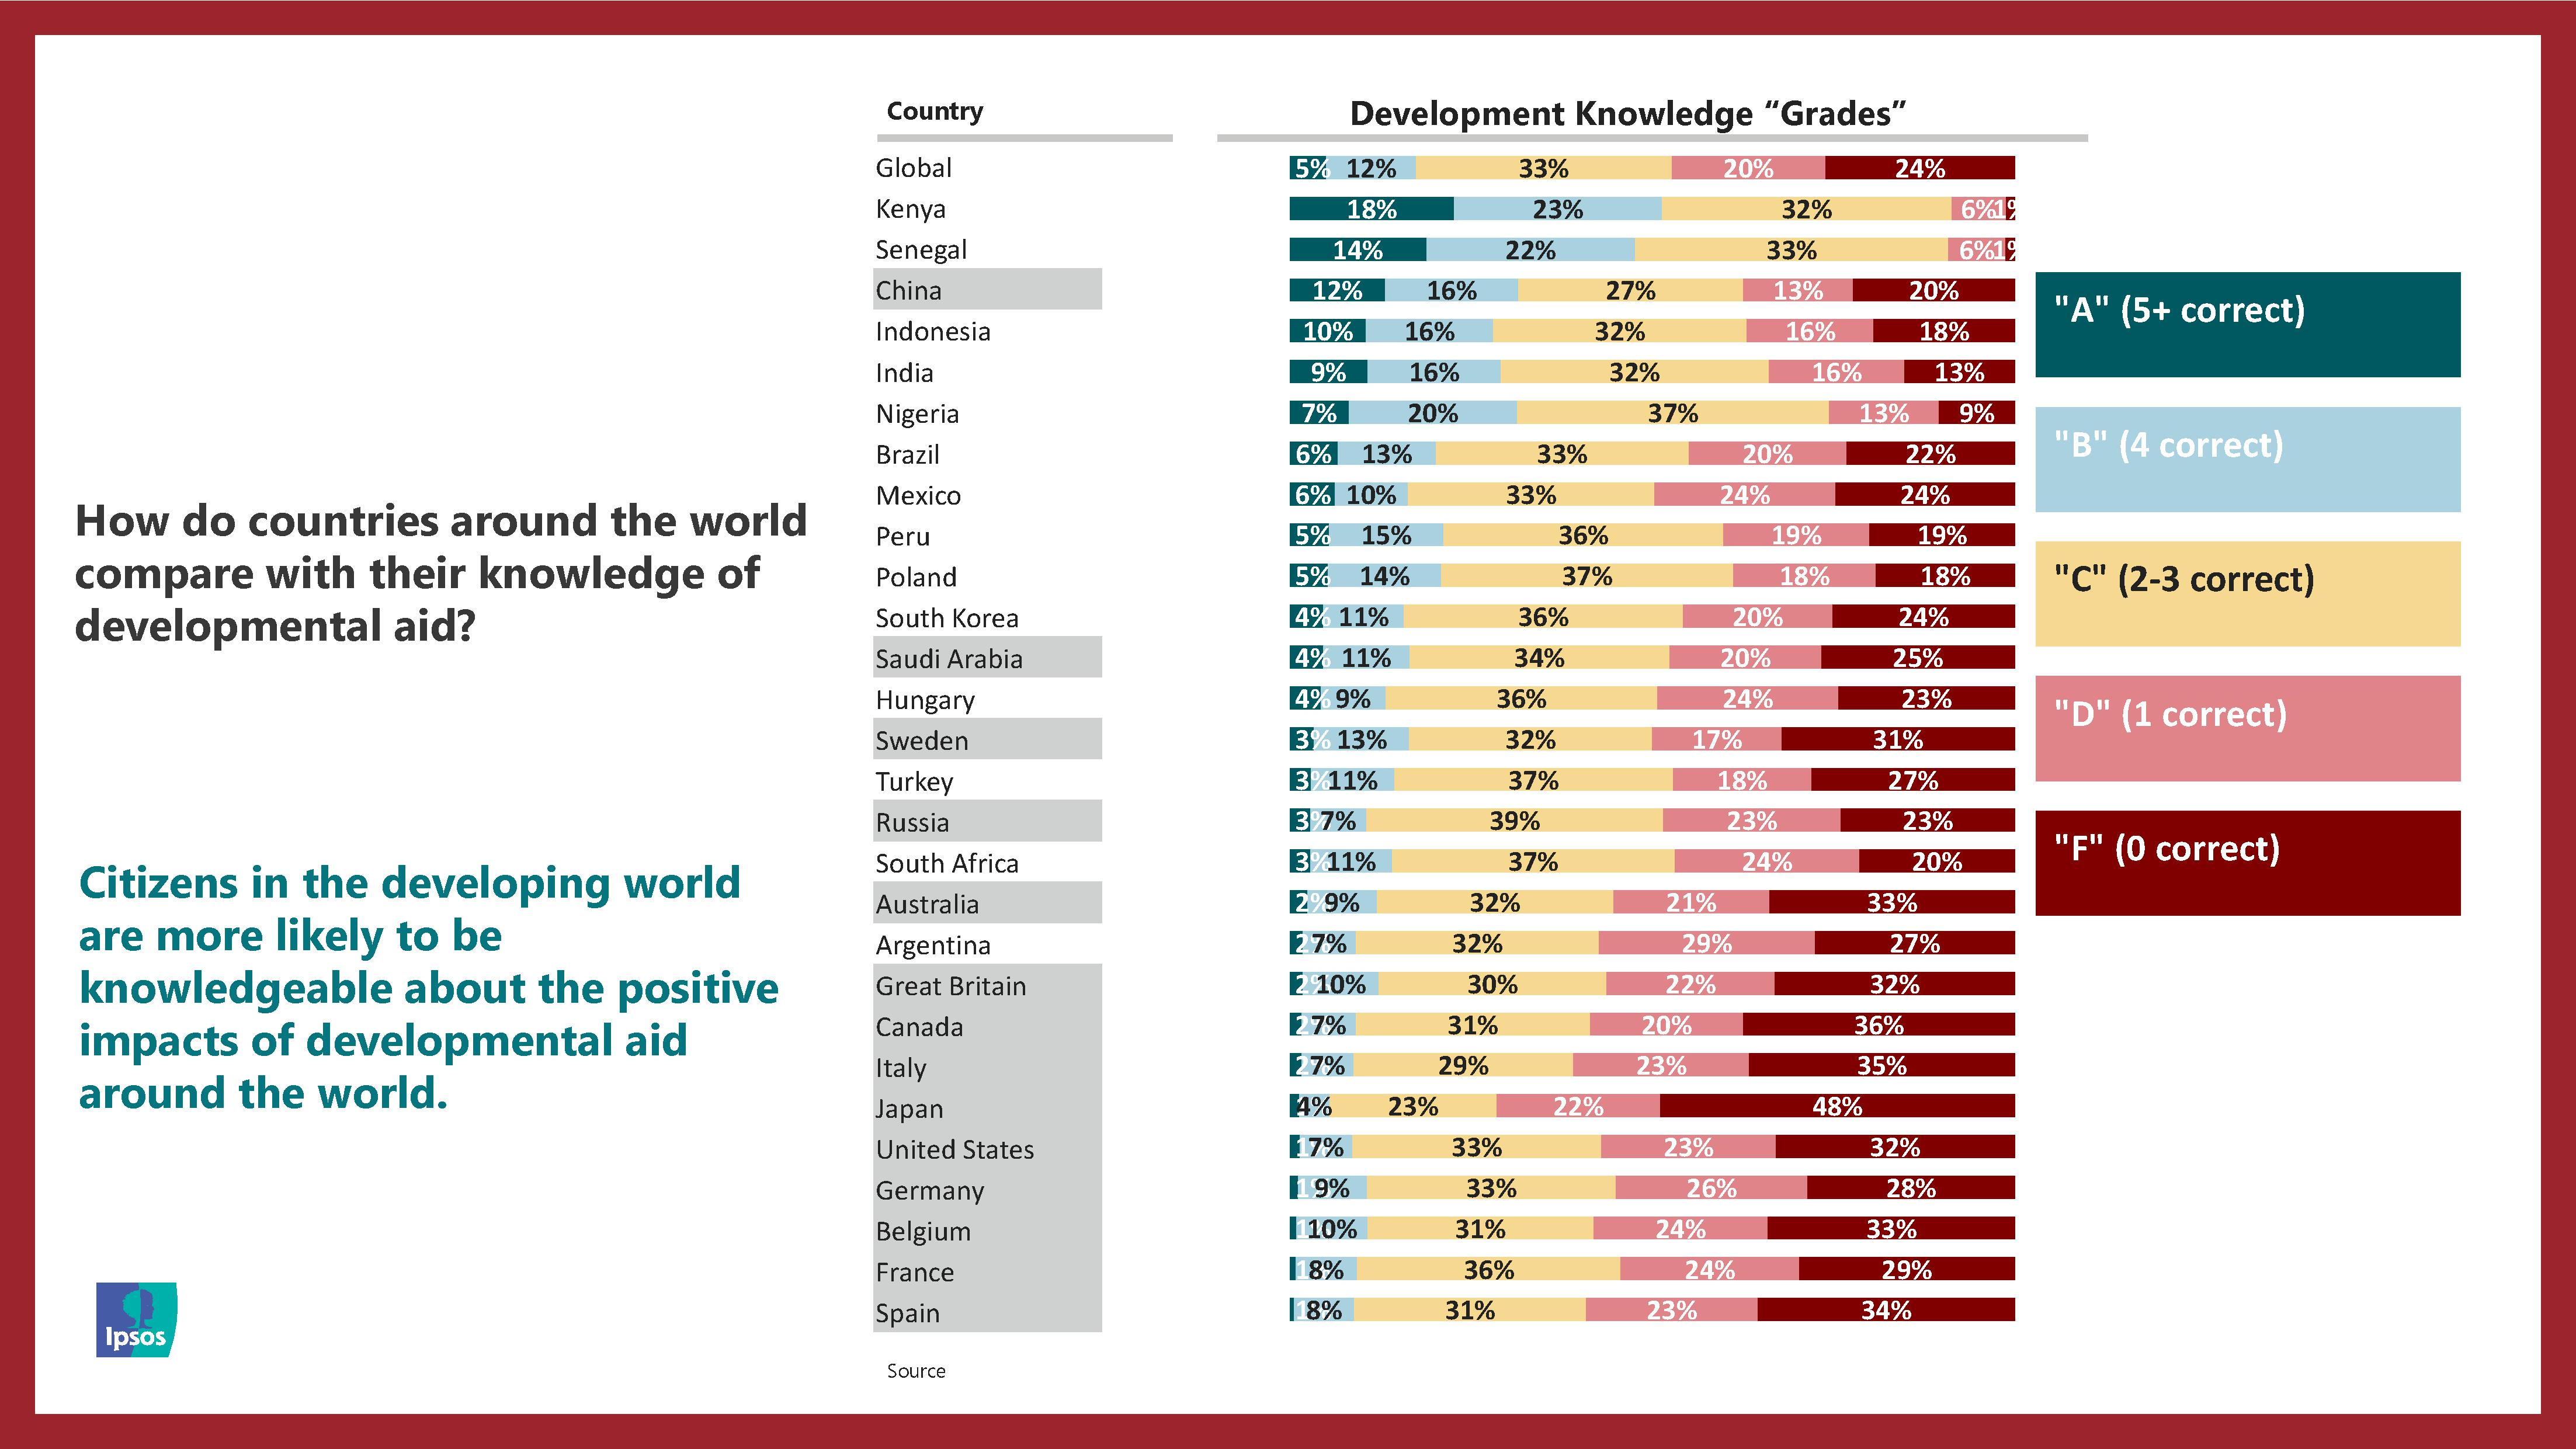
\includegraphics[width=\textwidth]{03MarcoTeorico/imageR/ipso}
	\caption{Gráfica global de la percepción de 28 paises respecto a la realidad. Donde vemos una gráfica que representa la cantidad de aciertos que tuvo la población por país en relación a la realidad.[Imagen](2017, Septiembre). Recuperado de https://www.ipsos.com/sites/default/files/ct/news/documents/2017-09/Gates\_Perils\_of\_Perception\_Report-September\_2017.pdf}
	\label{fig:ipso}
\end{figure}

\section{Consecuencias}
Ya que el desarrollo social y cultural están ligados, estos se encuentran también dependientes el uno del otro para su impulso. El movimiento cultural no solo favorecer el desarrollo recreativo si no que impulsa el desarrollo de sus naciones y viceversa. Tenemos como ejemplo en otros países del mundo, donde han sabido valorar las costumbres y tradiciones, he ahí donde nace el orgullo por su patria y se convierten en nacionalistas, demostrando el amor por su pueblo, marcando de manera definitiva el desarrollo científico, político y social de su nación\cite{pp06}.
\\[1pt]

La ignorancia cultural es el principal elemento que permite la injusticia, la enajenación y la explotación. Este fenómeno es sumamente grave y perjudicial para conformar lo que es la Identidad Cultural, la Identidad Nacional y la conciencia de la Nación. Al no saber quién es, cuáles son sus orígenes, su historia, su legado, su nombre, sus valores y principios, se le condena a la sociedad a permanentemente estar exaltando lo ajeno y despreciando lo propio.
\\[1pt]

En 2017, 41\% de los mexicanos no fue a ninguna actividad cultural según INEGI\cite{pp02}. La cifra podría leerse al revés: donde el 59\% del total de la población de 18 y más años de edad declaró que asistió a algún evento cultural seleccionado en los últimos doce meses. Pero cuando se trata de un país con una intensa vida cultural y artística, con más de 1,300 museos, alrededor de 178 zonas arqueológicas abiertas al público, 641 teatros y más de 4,000 salas de cine, de acuerdo con datos de la propia Secretaria de Cultura del gobierno federal\cite{pp01} al final queda que cuatro de cada diez personas no tienen como hábito la cultura a pesar de que varios de ellos son gratuitos.
\\[1pt]

Como ejemplo de la decadente autoconciencia cultural en México tenemos el día de la independencia. Quizá podría pensarse que todos los mexicanos saben que se festeja el 15 y 16 de septiembre. Sin embargo, los datos de la encuesta telefónica de Parametría\cite{pp03} muestran que 11\% de las personas no tiene idea de lo que se conmemora como se ve en la gráfica \ref{fig:enc01} y 57\% no sabe de que país se independizó como se ve en la gráfica \ref{fig:enc02}. Adicionalmente como podría esperarse, el nivel de escolaridad influye en el conocimiento que se tiene sobre el tema. Así, puede observarse que conforme aumenta el nivel de escolaridad se incrementa el conocimiento sobre la celebración de independencia y también sobre el país del cual se independizó México según la gráfica. \ref{fig:enc03}.
\\[1pt]

\begin{figure}
	\centering 
	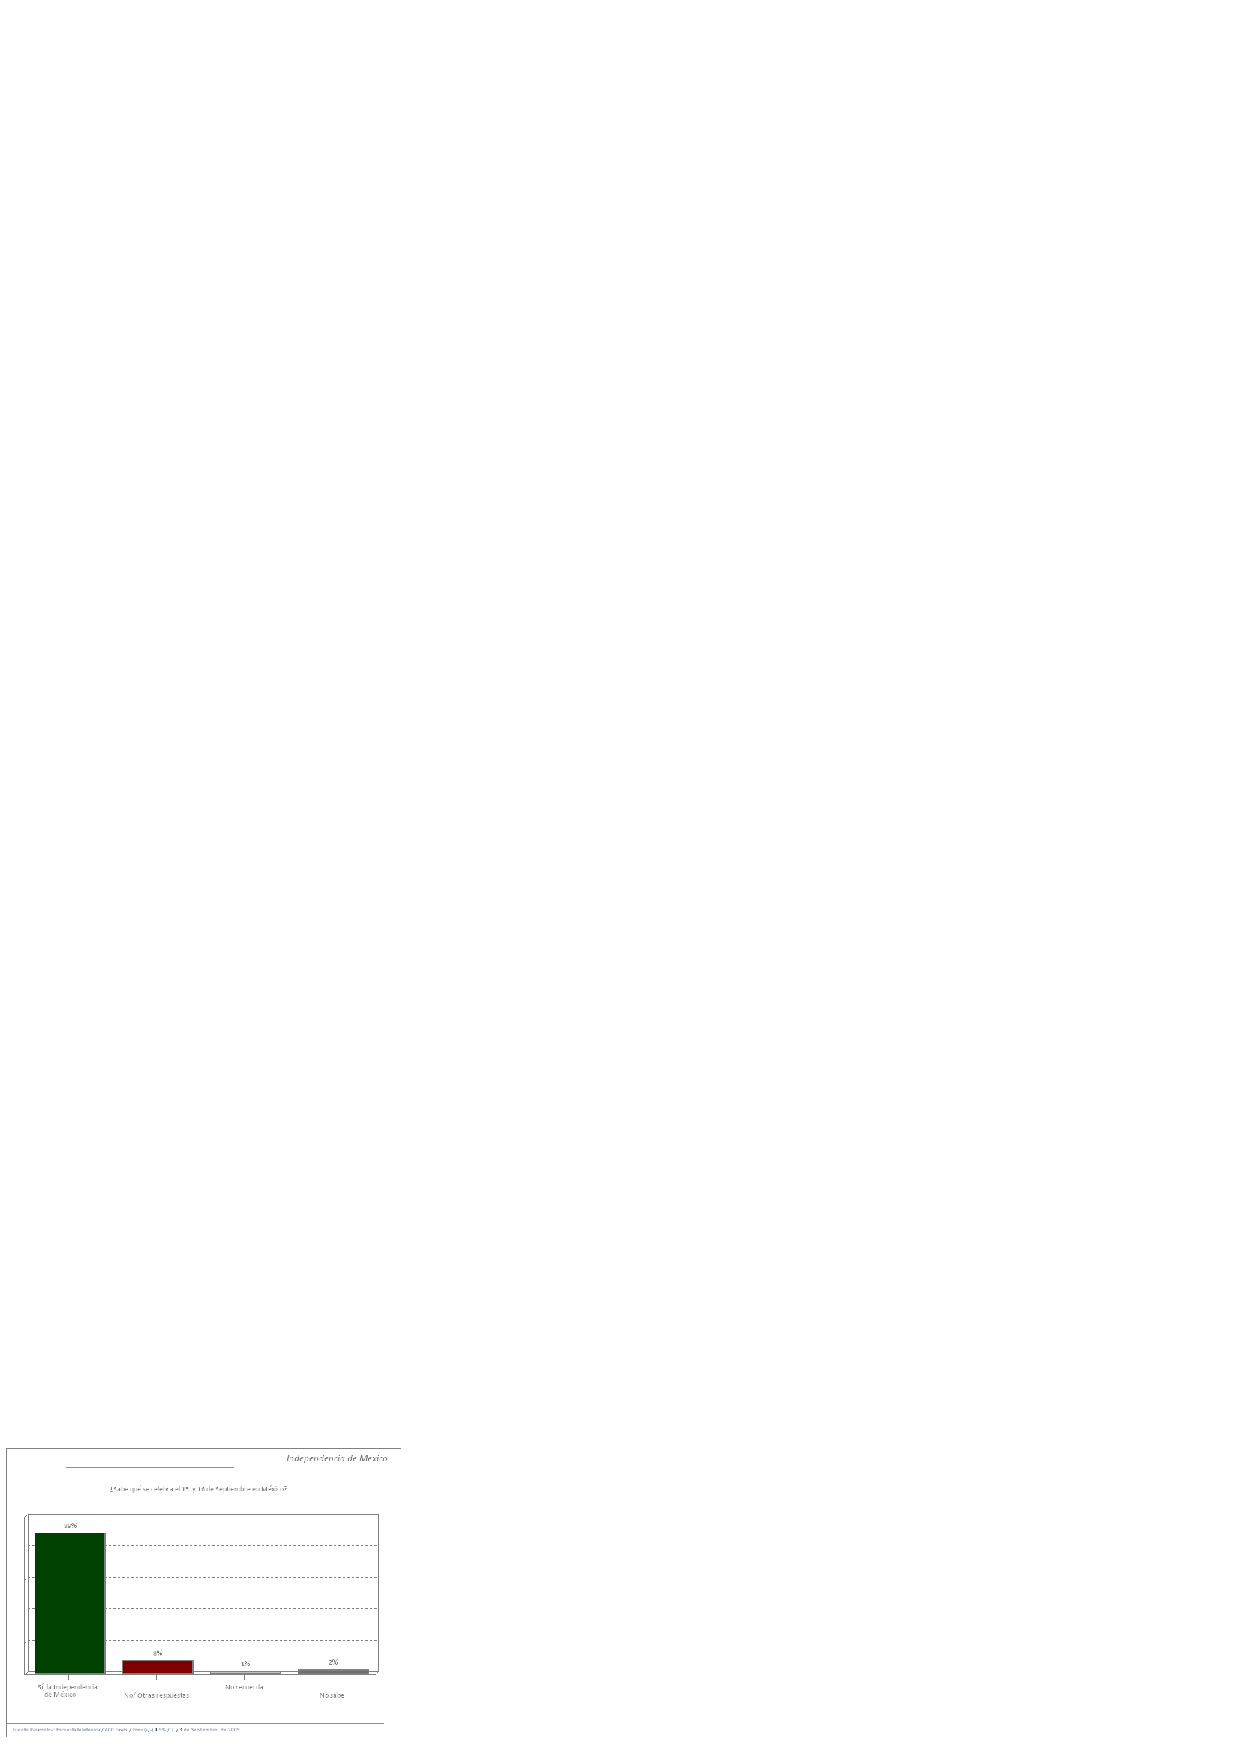
\includegraphics[width=.50\textwidth]{03MarcoTeorico/imageR/enc01}
	\caption{Gráfica a la pregunta ¿Sabe que se celebra el 15 y 16 de Septiembre en México?[Imagen](2009, Septiembre). Recuperado de: http://www.parametria.com.mx/carta\_parametrica.php?cp=4170.}
	\label{fig:enc01}
\end{figure}

\begin{figure}
	\centering 
	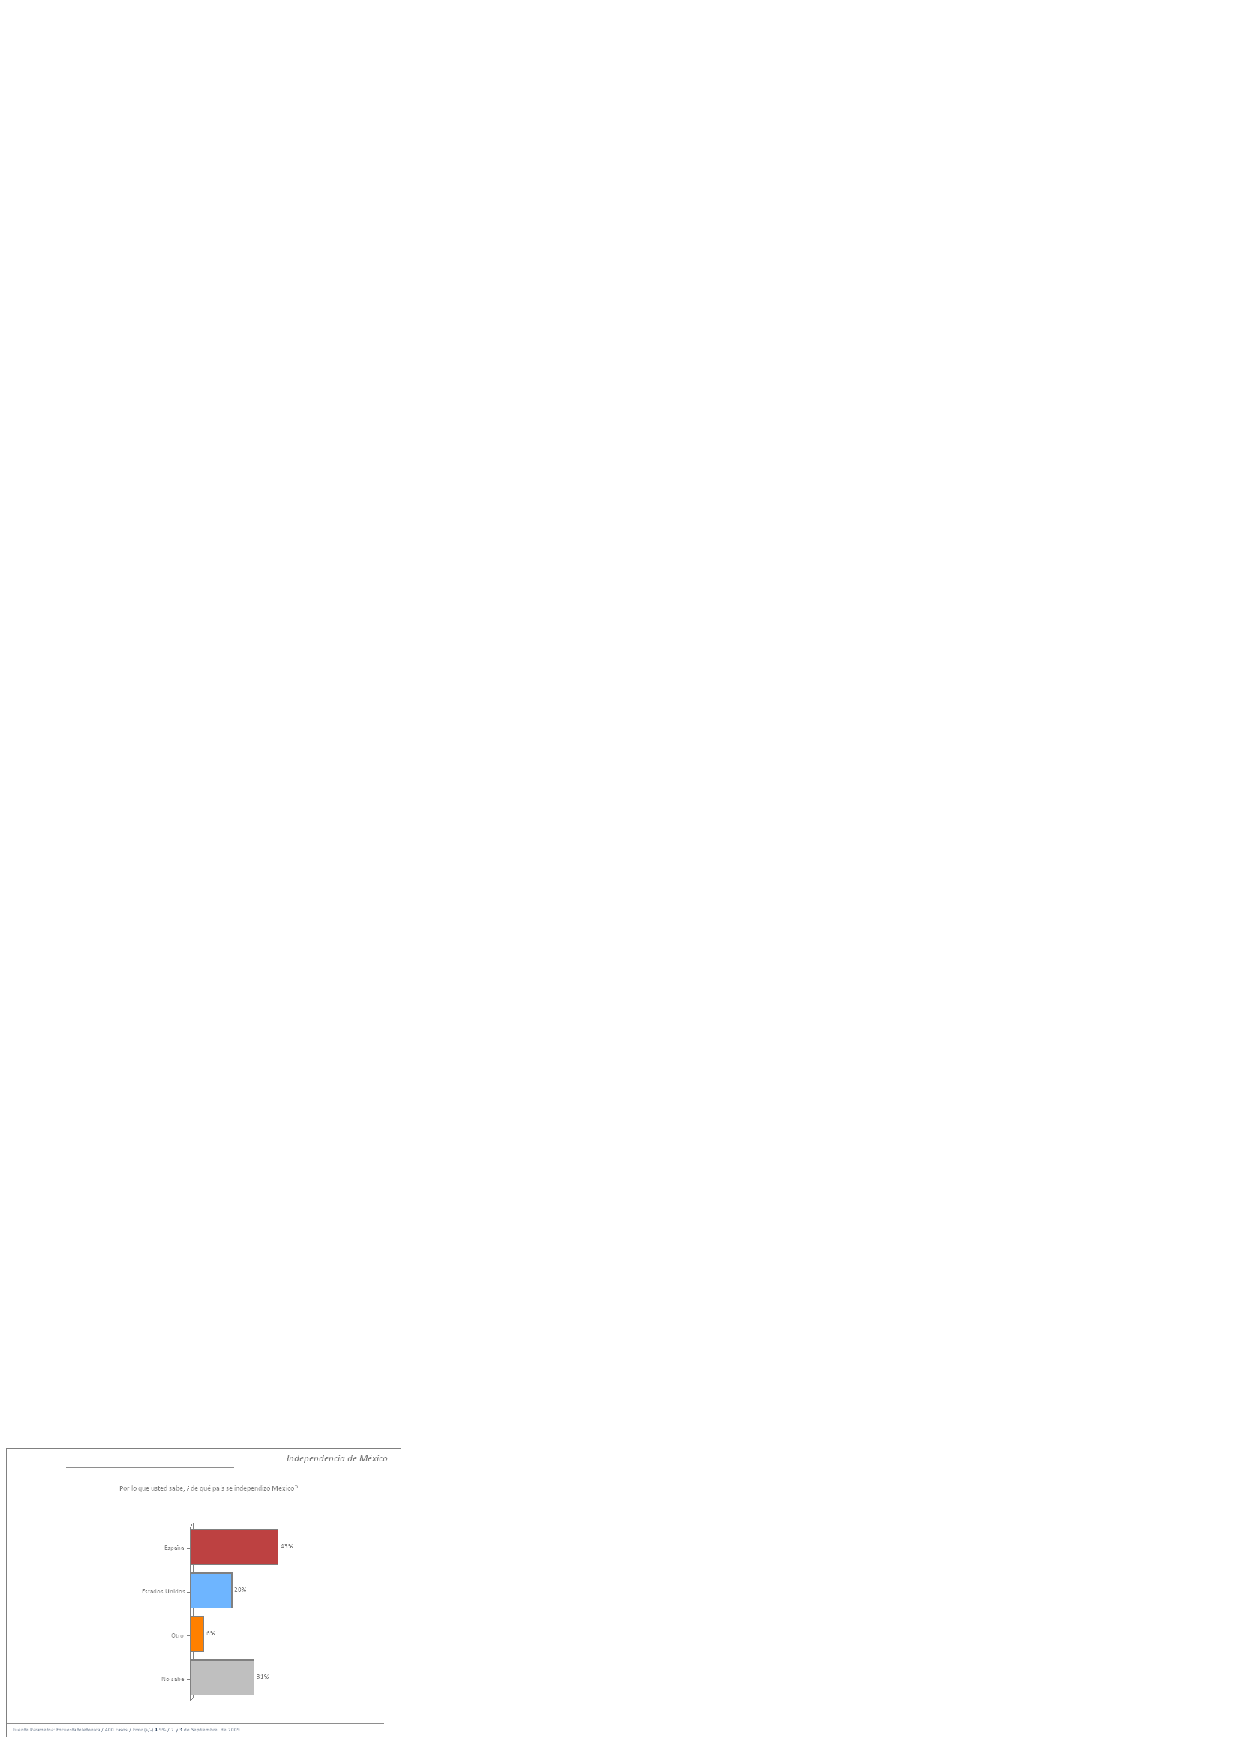
\includegraphics[width=.5\textwidth]{03MarcoTeorico/imageR/enc02}
	\caption{Gráfica a la pregunta ¿De que país se independizó México?[Imagen](2009, Septiembre). Recuperado de: http://www.parametria.com.mx/carta\_parametrica.php?cp=4170.}
	\label{fig:enc02}
\end{figure}

\begin{figure}
	\centering 
	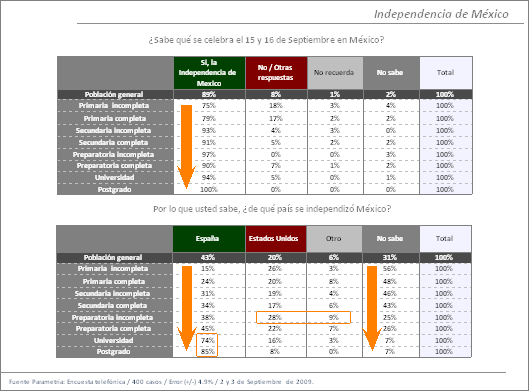
\includegraphics[width=.5\textwidth]{03MarcoTeorico/imageR/enc03}
	\caption{Gráfica de como influye la escolaridad en el conocimiento que se tiene de las fiestas patrias[Imagen](2009, Septiembre). Recuperado de: http://www.parametria.com.mx/carta\_parametrica.php?cp=4170.}
	\label{fig:enc03}
\end{figure}

Debemos saber cuál es nuestra verdadera herencia cultural y cuál nuestro legado, para preservarlo y desarrollarlo. Y como dice Guillermo Marín \cite{pp07} ``Este país se tiene que encontrar a sí mismo".
\\[1pt]


\section{Propuesta de solución}
Propondremos como solución el crear un videojuego con contexto histórico y mitológico del país prehispánico mexicano. Para esto el factor de entretenimiento y diversión lo sobrepondremos al del conocimiento o educativo.
\\[1pt]

%%%%%%%%%%%%%%%%%%%%%%%%%5YA EXISTE?
Como ejemplo similar tomaremos el videojuego llamado ``Assasins Creed II" lanzado en el año 2009, que debutó en el puesto número 1 en Estados Unidos, Canadá, Suecia, Francia, España y Australia, y dentro del «Top 50» en más de diez países. Este juego tiene como género acción-aventura, también se situa en la época renacentista y este hecho lográ que el jugador adquiera conocimientos sobre ese tiempo, tanto lugares, como personas, situación social, etc.
\\[1pt]

%%%%%%%%%%%%%%%%%%%%%%%%%%55QUE IMPLICA?
Para llevar a cabo el diseño de un videojuego los programadores son los responsables de hacer posible la interactividad entre el jugador y el sistema. Se realizará detro del proyecto la programación estructurada, orientada a objetos, modelado, arte digital, conocimiento de dispositivos móviles y animación digital. Considerando importante usar modelos matemáticos para las diferentes experiencias de juego. 
\\[1pt]

%%%%%%%%%%%%%%%%%%%%%%%%%%%%%%%VENTAJAS?
El resultado de adquisición de conocimiento en lo videojuegos se debe al cómo. En la imagen \ref{fig:conoAprendizaje} se muestra el cono de la experiencia de Edgar Dale (pedagogo) donde resaltamos que el mayor aprendizaje es por medio de la simulación.

\begin{figure}
	\centering 
	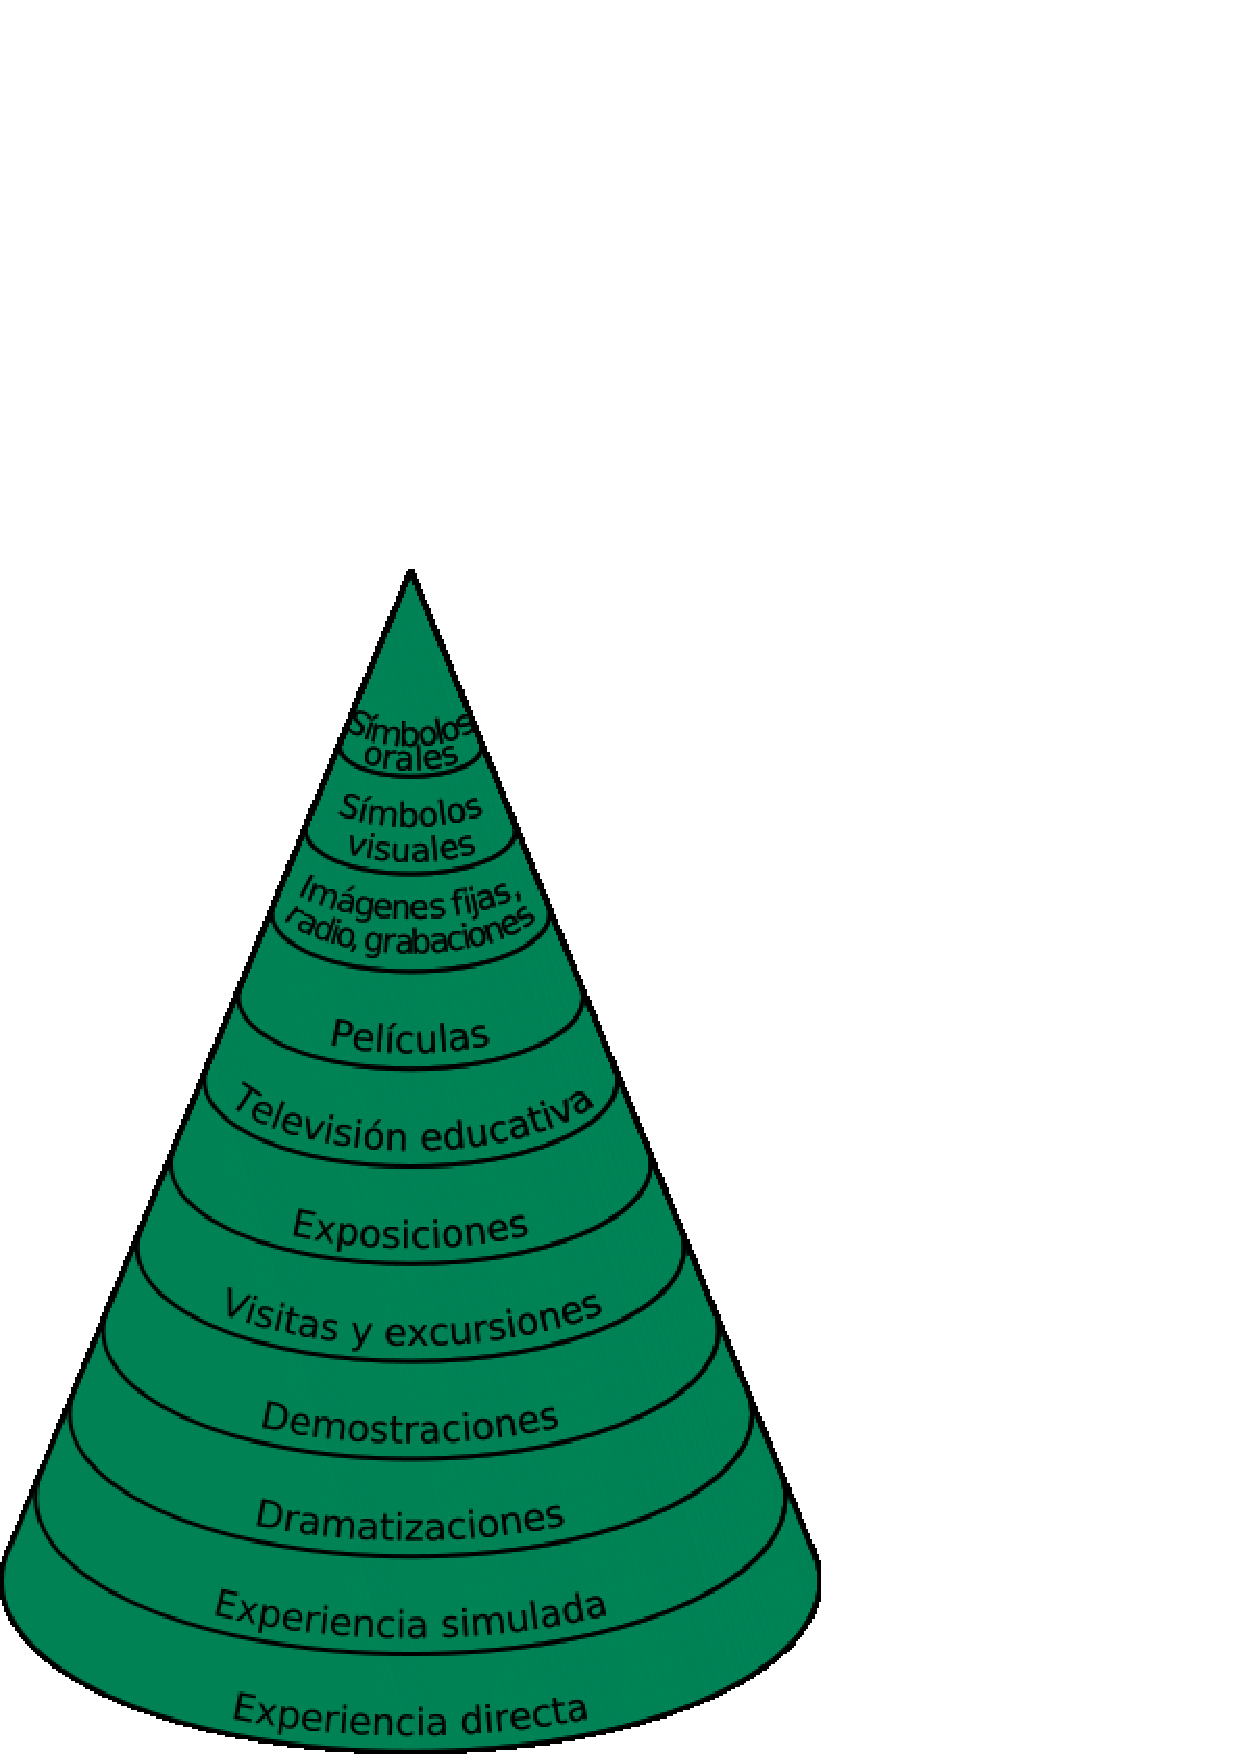
\includegraphics[width=.5\textwidth]{03MarcoTeorico/imageR/conoAprendizaje}
	\caption{Cono de la experiencia de Edgar Dale. Se muestra diferentes maneras de aprendizaje que se ordenan según su impacto de aprendizaje.[Imagen](2008). Recuperado de: https://es.wikipedia.org/wiki/Edgar\_Dale\#/media/File:Cono\_de\_la\_Experiencia.svg}
	\label{fig:conoAprendizaje}
\end{figure}

Los medios audiovisuales son los que mayor impacto tiene en difusión cultural como se ve en la gráfica de la imagen \ref{fig:modecult}. Así podemos ver una potencial herramienta para insitar a la participación en los eventos culturales, pues los videojuegos son medios audiovisuales.
\\[1pt]

\begin{figure}
	\centering 
	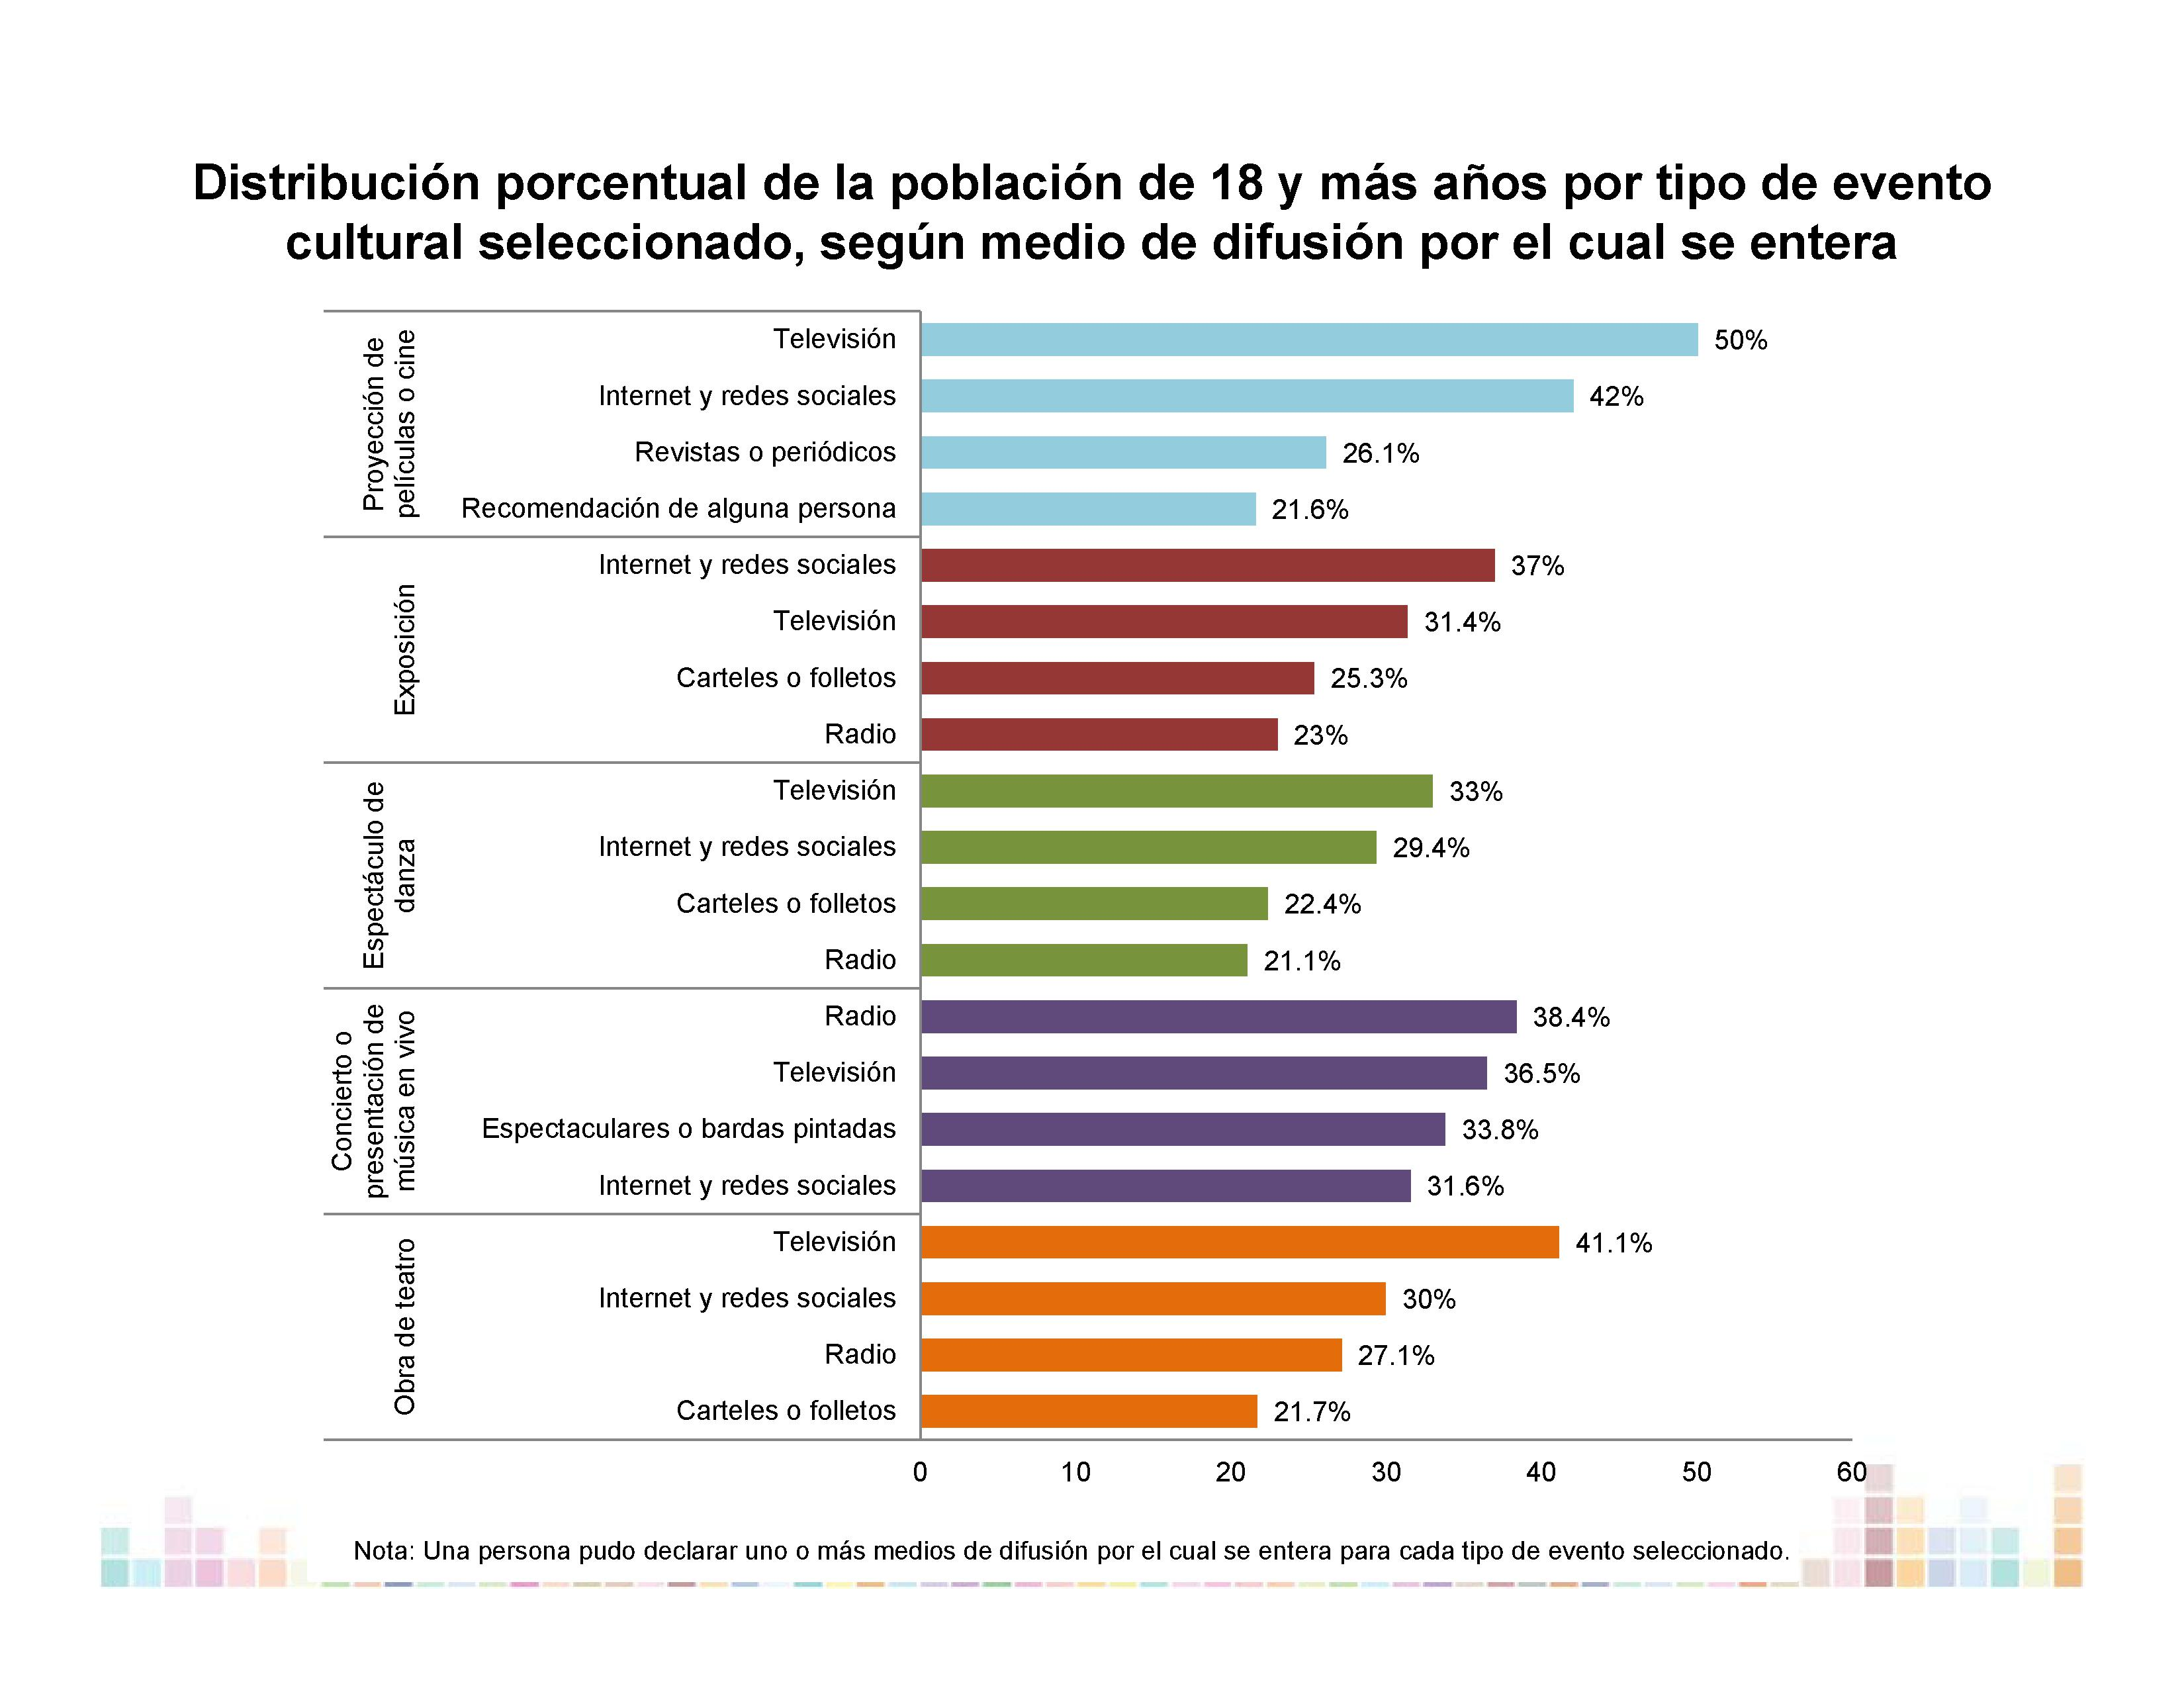
\includegraphics[width=.75\textwidth]{03MarcoTeorico/imageR/modecult}
	\caption{Encuesta MODECULT en asistencia por tipo de evento y medio de difusión por el cual se ha enterado.[Imegen](2017, Mayo). Recuperado de: http://internet.contenidos.inegi.org.mx/contenidos/productos/prod\_serv/contenidos/espanol/bvinegi/productos/nueva\_estruc/promo/resultados\_modecult\_may2017.pdf}
	\label{fig:modecult}
\end{figure}

También otra de las ventajas es la cantidad de gente que juega videojuegos en México y el dispositivo por el cuál lo consumen como lo muestra la imagen \ref{fig:consumo30}. Donde el 20\% de los mexianos consumen videojuegos y 45\% de ellos se juegan en dispositivos móviles.

\begin{figure}
	\centering 
	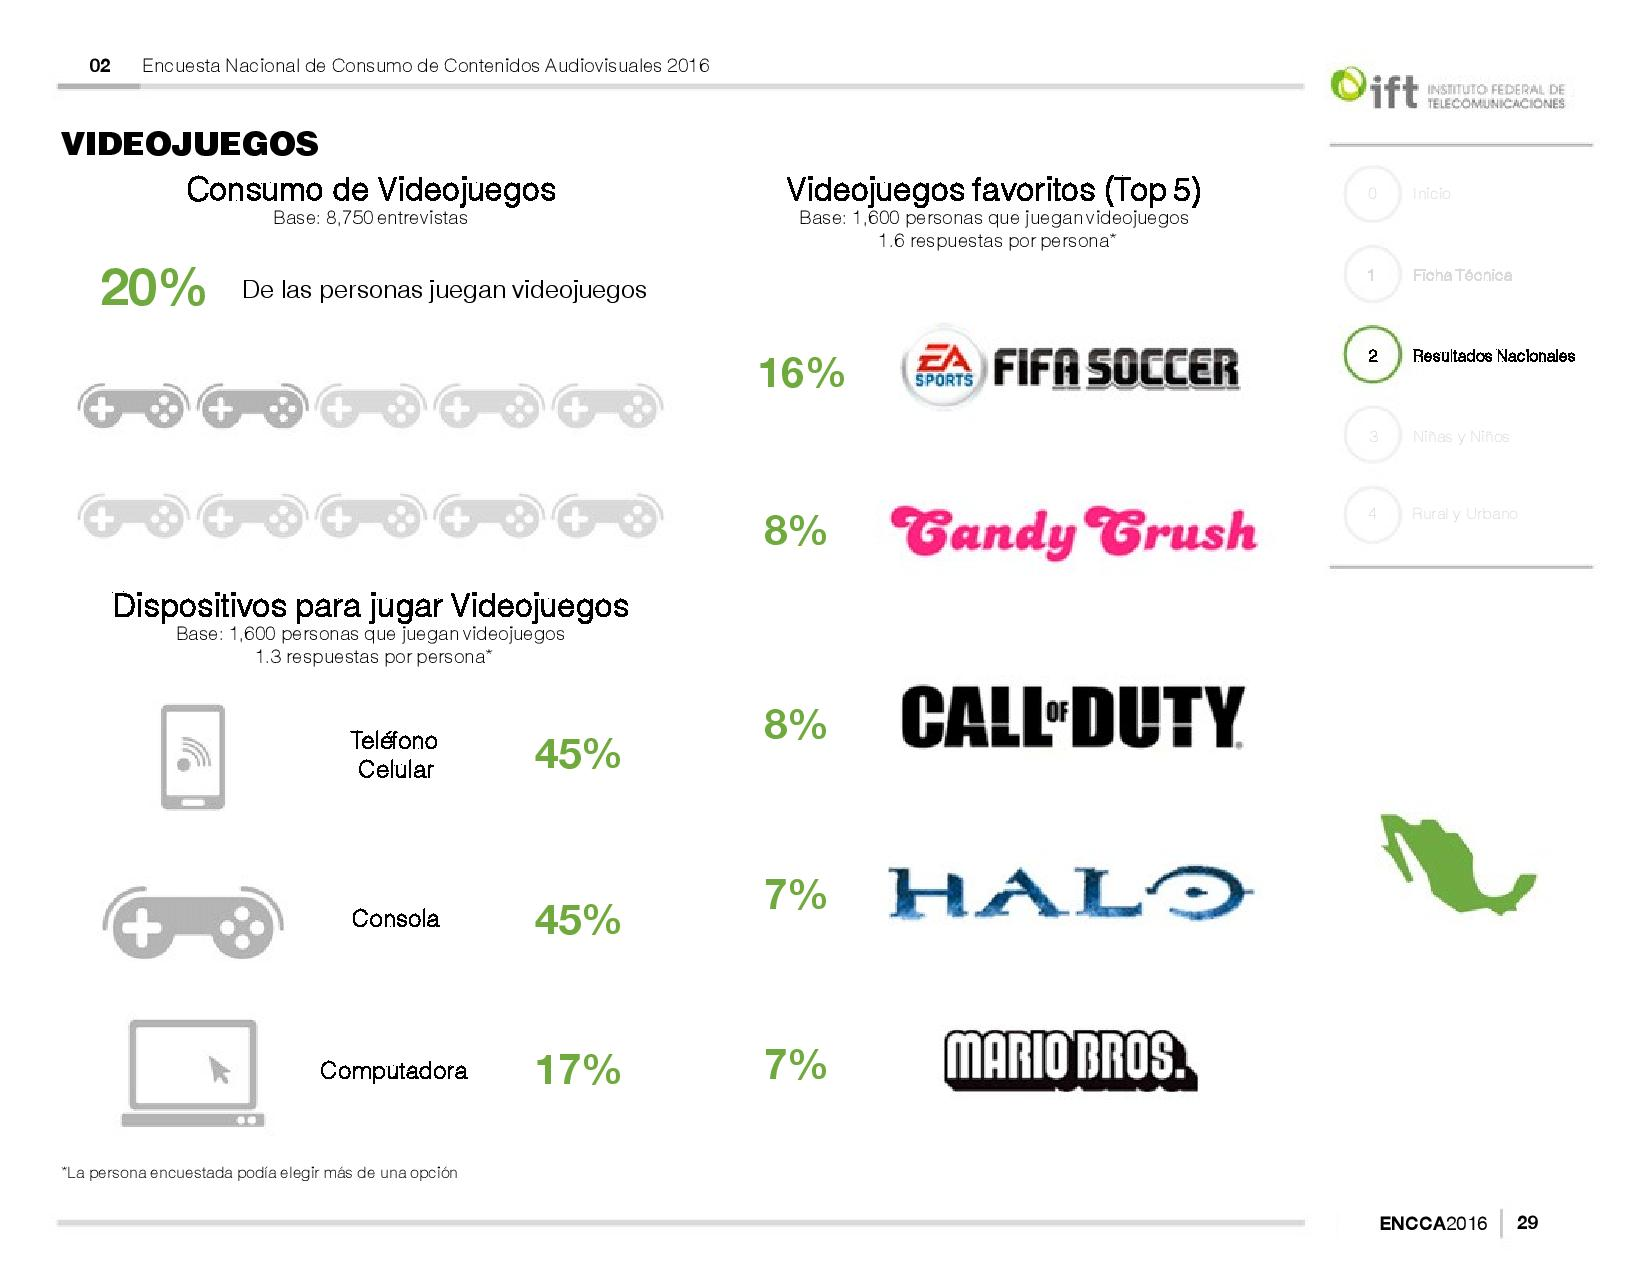
\includegraphics[width=.75\textwidth]{03MarcoTeorico/imageR/consumo30}
	\caption{Encuesta Nacional de Consumo de Contenidos Audiovisuales, donde muestra el consumo de videojuegos[Imegen](2016). Recuperado de: http://www.ift.org.mx/sites/default/files/encca2016\_vf-compressed.pdf}
	\label{fig:consumo30}
\end{figure}

%%%%%%%%%%%%%%%%%%%%%%%%%%DESVENTAJAS?

Una desventaja de los videojuegos en cuestión de desarrollo es que son un complejo sistema tecnológico que combina diversos elementos: visuales, matemáticos, físicos, electrónicos o narrativos, entre otros muchos para generar una experiencia controlada porel jugador para su mayor entretenimiento. Por tanto existe una complejidad al unir de forma adecuada todos esos elemntos para crear una gran experiencia de diversión para los jugadores, se necesita de una gran cantidad de talentos diversos o multidisciplinarios, los cuales no se abarcarán todos ellos.

También se debe tomar en cuenta que existe una gran cantidad de gustos e intereses entre los jugadores existentes y no se puede aplicar todos los existentes.

La mejora de las condiciones de un producto en un videojuego resulta esencial. Por esta misma razón el tiempo de desarrollo siempre es muy largo y en la mayoría de las ocasiones tiene muchos contratiempos que provocan retrasos de lanzamiento o incluso rediseños completos.




	%\chapter{Marco teórico conceptual}
	\section{Videojuegos}
\subsection{Definición}
\subsection{Clasificación}
\subsection{Industria en México}

	\section{Desarrollo de videojuegos}
	En sus inicios los videojuegos se encontraban fuertemente ligados al hardware y no eran los complejos sistemas actuales; por lo tanto, la naciente industria de los videojuegos no tenía la necesidad de documentar sus productos como sistemas de software. Es a partir de la segunda mitad de la década de los 80’s con la llegada de Nintendo que el videojuego da sus primeros pasos como sistema complejo de software [ ]. Si bien Nintendo inicio el videojuego como medio argumental y de entretenimiento, no fue esta compañía la que iniciaría la producción sistematizada del videojuego, tal merito se lo lleva la compañía ID Software con el lanzamiento de Doom en la década de los 90’s, siendo el primer videojuego diseñado bajo una arquitectura orientada a la reutilización. Dicha arquitectura consistía en separar el software en una serie de módulos con funcionalidad especifica de tal suerte que dichos módulos se pudieran reutilizar en proyectos de temática parecida sin que se tuviera que modificar directamente el código, limitando al equipo de programadores únicamente a agregar módulos nuevos que complementaran la funcionalidad [ ]. Naciendo así la necesidad de documentar los videojuegos como sistemas de software. La década de los 90’s es un segundo punto de inflexión en la industria, pues hasta ese momento el mercado había sido dominado por compañías como Nintendo y SEGA. En 1994 PlayStation de la compañía SONY llega al mercado de los videojuegos y con esta consola se abre la puerta a títulos de carácter más maduro, iniciando así la masificación de los videojuegos [ ]. Con la llegada de las computadoras personales, el XBOX de Microsoft y el boom del internet la industria del videojuego volvió a adaptarse al mercado. 
\\
\par
Del anterior párrafo puede concluirse que la industria de los videojuegos tuvo que pasar por diferentes cambios para comenzar a implementar metodologías de desarrollo de videojuegos y herramientas que le permitieran a las compañías optimizar recursos y tiempos[ ]. 
\subsection{Metodologías de desarrollo}

\input{03MarcoTeorico/03DesarrolloVideojuego/Metodologias/01Cascada}
\input{03MarcoTeorico/03DesarrolloVideojuego/Metodologias/02Scrum}
\input{03MarcoTeorico/03DesarrolloVideojuego/Metodologias/03XP}
\input{03MarcoTeorico/03DesarrolloVideojuego/Metodologias/04Huddle}



	\subsection{Pipeline}
	\subsection{Motores gráficos}
	\input{03MarcoTeorico/03DesarrolloVideojuego/MotoresGraf/01motorGrafico}
	\input{03MarcoTeorico/03DesarrolloVideojuego/MotoresGraf/02ArqutecturaMotor}
	\input{03MarcoTeorico/03DesarrolloVideojuego/MotoresGraf/03Motores}
	\subsection{Software auxiliar}
	\section{Gamificación}
La gamificación es el uso de las mecánicas de juego en entornos ajenos al juego, según el término anglosajon definido por Sebastian Deterding (Diseñador/investigador del diseño de juego para el florecimiento humano) \cite{gameDef}. Es decir, que cualquier tema o asunto a tratar puede pasar por un proceso para convertirse en un juego. Y deben de cumplir con características específicas según el profesor Santiago Moll\cite{gameficacion}, estas son: mecánicas o reglas, dinámicas de juego, y componentes. También describe que clase de jugadores existen, el proceso que debe de llevar un tema a gamificar y la finalidad que debe cumplir. Todo esto se muestra a continuación.
\\[1pt]

\subsection{Característcas}
Las características a presentar son una guía para realizar un juego y no necesariamente se debe cumplir con todas y cada una de ellas. Sin embargo estas características ayudan en gran medida al entretenimiento del jugador. Recordemos que las características a presentar incluyen las mecánicas o reglas, dinámicas de juego y componentes.
\\[1pt]
 
\textbf{Mecánicas o reglas}
\\[1pt]
Son las normas de funcionamiento que permiten se adquiera un compromiso del jugador con el juego. Mantienen al jugador en constante actividad y le permite ver los límites que existen en el juego.
\\[1pt]

\begin{itemize}
	\item Colección: Logros y recompensas que consigue el jugador.
	\item Puntos: Para motivación y conteo de realizar una tarea por el jugador.
	\item Ranking: Clasificación o comparación entre jugadores.
	\item Nivel: Reflejan el progreso del jugador.
	\item Progresión: Consiste en completar el 100\% de la actividad encomendada al jugador.	
\end{itemize}

\textbf{Dinámicas de juego}
\\[1pt]
Motivan y despiertan el interés del jugador de realizar una actividad dentro del juego. Aunque no es necesario cumplir con este requisito para un juego son clave para mantener jugando a la persona.  

\begin{itemize}
	\item Recompensa: Premio por realizar alguna actividad en el juego.
	\item Competición: Deseo de estar en una determinada posición o grado en el juego entre los participantes.
	\item Cooperativismo: Otra forma de competir pero en un grupo de jugadores con un mismo fin o meta del juego.
	\item Solidaridad: Se fomenta la ayuda entre jugadores y debe ser de manera altruista.
\end{itemize}

\textbf{Componentes}
\\[1pt]
Los componentes se encargan de personalmente darle a cada jugador su estado en el juego. Así son identificados por los demás participantes fácilmente en las actividades que destacan o han realizado con exito. También cumplen con la parteen la que el jugador puede proyectarse dentro juego.
\begin{itemize}
	\item Logros: Visualizan el alcance del jugador de un objetivo del juego.
	\item Avatares: Representación gráfica del jugador.
	\item Medallas: Insignia o distintivo del jugador que ha ganado.
	\item Desbloqueo: Permiten avanzar en las actividades del juego gracias a actividades previas hechas por el jugador.
	\item Regalos: Un presente por la realización correcta de un reto por el jugador	.
\end{itemize}

\subsection{Tipos de jugadores}
Para saber que elementos debe llevar el juego a realizar debe conocerse los tipos de jugadores que existen. También se debe de saberse las motivaciones que los impulsan a seguir jugando. A continuación se muestran cuatro identificados.
\begin{itemize}
	\item Triunfador: Su finalidad es la consecución de logros y retos.
	\item Social: Le encanta interactuar y socializarse con el resto de compañeros.
	\item Explorador: Tiene tendencia a descubrir aquello desconocido.
	\item Competidor: Su finalidad es demostrar su superioridad frente a los demás.
\end{itemize}


\subsection{Proceso}
Ahora se seguirá los pasos para convertir un tema a un juego. Conociendo ya los elementos que disponemos y haber identificado al tipo de jugador que queremos, podemos convertir nuestro tema o actividad en un juego. 
\begin{itemize}
	\item Viabilidad: Determinar si el contenido que se quiere enseñar es jugable.
	\item Objetivos: Definir los objetivos del juego.
	\item Motivación: Valorar la predisposición y el perfil de jugadores.
	\item Implementación: Relación entre el juego y contenido a enseñar.
	\item Resultados: Evaluación de la actividad en el juego.
\end{itemize}


\subsection{Finalidad}
En cada juego se debe tener claro lo que quiere lograrse, es decir la finalidad del juego. Debe de determinarse que se desea lograr con el jugador.
\begin{itemize}
	\item Fidelización: Establecer un vínculo del contenido del juego con el jugador.
	\item Motivación: Crear una herramienta contra el aburrimiento del contenido a tratar.
	\item Optimización: Recompensar al jugador en aquellas tareas en las que no tiene previsto ningún incentivo.
\end{itemize}

	\section{Cultura}

	\section{Cultura Digital}
La misión de la cultura digital es generar a través del espacio físico y de plataformas virtuales, programas enfocados al uso creativo y crítico de la tecnologías digitales como herramientas de producción y transformación cultural \cite{vid08}. El objetivo ha ido precisamente cubrir el déficit de investigación que hay sobre cultura del ocio juvenil vinculado a las nuevas tecnologías, justamente cuando estas prácticas alcanzan una importancia cada vez mayor, no sólo por el perfeccionamiento de las tecnologías, ni por el incremento de su uso, sino precisamente por su papel en las relaciones de consumo.
\\[1pt] 

Las definiciones de consumo cultural que no tengan en cuenta el uso de las nuevas tecnologías perderán rápidamente la capacidad de definir lo que podrían ser aceptables y asumibles por parte de la sociedad. En el proceso de consumo es crear identidad de nuevas tecnologías de información y comunicación, que efectúan los y las adolescentes en los espacios de ocio, así es posible reconocer la creación de una nueva cultura digital. Ésta se puede observar a través de las prácticas específicas que se producen y que van mucho más allá del simple uso de la conexión.
\\[1pt]

La generación educada en este inicio de siglo XXI es audiovisual, lo que la caracteriza es que emergen ya en el interior de una cultura digital, es una generación que llegará a la mayoría de edad "bañada en bits".Se subraya la importancia de estudiar la cultura de esta generación, las maneras en que se relacionan, ya que es en estos procesos donde se pueden adivinar los cambios en la sociedad, las nuevas concepciones del trabajo y las ideologías del futuro.
\\[1pt]

\subsection{Educación digital}
Los estudiantes en estos nuevos modelos actúan cada vez más como socios y pares del profesor en la construcción de conocimiento como una estrategia de aprendizaje. Los estudiantes han de participar activamente en el proceso de aprendizaje, y colaborar tanto entre ellos como con los profesores trabajando tanto individualmente como en equipo. La transición de sistemas cerrados a abiertos y de arquitecturas centralizadas a distribuidas facilita el fortalecimiento del aprendizaje en las que se prima la iniciativa del estudiante y sus capacidades creativas e innovadoras.
\\[1pt] 

Las redes de interés, de alcance global y donde se relacionan con otras personas de intereses similares, independientemente de su localización geográfica, es donde se desarrollan especialmente las capacidades creativas y proporcionan un canal para ganar visibilidad y reputación entre sus pares. En las redes de interés, surgen formas de participación que conforman un aprendizaje informal, al margen de las instituciones educativas, basado en la colaboración con otros usuarios y en el ensayo y error, la exploración y el bricolaje. 
\\[1pt]

Por tanto, los jóvenes adquieren, sus competencias y habilidades tecnológicas en estos espacios informales donde su actividad es social y apasionada. A diferencia del aula, los jóvenes prefieren los espacios digitales por la autonomía y libertad que les proporciona, y porque el estatus y la autoridad vienen determinados por sus habilidades y no por una jerarquía preestablecida\cite{vid09}.
\\[1pt]


	
	\section{Videojuegos lúdicos}

Los videojuegos se utilizan como herramienta educativa que permite a los estudiantes desarrollar competencias en sus procesos de aprendizaje. Informes del Horizon (New Media Consortium) como \cite[Games and gamification]{vid07} resaltan la gamificación como una de las principales herramientas de aprendizaje con mayor crecimiento.
\\[1pt]

Instintivamente, el ser humano aprende jugando. Desde los primeros años de vida el niño adquiere conocimientos a través del juego. Para la psicóloga infantil, esta característica permite al infante socializar en un entorno completamente nuevo, que lo estimula a conocer muchos aspectos de la realidad. Además de ser emocionante y entretenido le permite desarrollar un nivel de pensamiento creativo para enfrentar las circunstancias de la vida. El adulto tiene temor a equivocarse, mientras que un niño juega, se equivoca, lo vuelve a intentar, y de esa experiencia aprende.
\\[1pt]

El videojuego se puede utilizar como un instrumento del proceso enseñanza-aprendizaje. Según lo anterior por el Dr. Francisco Revuelta, especialista en procesos de formación en espacios virtuales dentro del ámbito pedagógico, este es dividido en dos vertientes. La primera, como un simulador de aprendizaje o herramienta en el cual se puede comprobar el nivel de competencia del alumno de acuerdo a las exigencias que le propone el videojuego. La segunda, como un entorno virtual de aprendizaje donde el estudiante es motivado a resolver problemas académicos interactuando dentro del espacio brindado por el videojuego\cite{vid06}.
\\[1pt]

Dentro de la gamificación el videojuego aumenta la motivación en el aprendizaje, ayuda al alumno a adquirir conocimientos de una manera atractiva y contribuye al desarrollo de competencias. Para que el alumno aprenda, el docente debe plantearse, como primer paso, qué es lo que quiere enseñar y, de acuerdo a esto, se busca un videojuego que sirva de instrumento para motivar el aprendizaje. El videojuego aumenta la motivación en el aprendizaje, ayuda al alumno a adquirir conocimientos de una manera atractiva y contribuye al desarrollo de competencias, pero sólo sirve como complemento de las herramientas básicas en el proceso de enseñanza-aprendizaje. 
\\[1pt]

	
				
		
		
		
	%\chapter{Estado del arte}

\begin{table}[]
	\centering
	\caption{Comparativa con juegos similares}
	\label{tableEA}
	
	\resizebox*{\textwidth}{!}{
		\begin{tabular}{|l|l|l|l|l|l|l|l|l|l|l|l|l|l|l|l|l|l|l|l|l|l|l|}
			\hline
			\multicolumn{1}{|c|}{\multirow{2}{*}{Juego}} & \multirow{2}{*}{Fecha} & \multicolumn{8}{c|}{Género}                                                    & Edad  & \multicolumn{5}{c|}{Plataforma}                    & \multicolumn{3}{c|}{Tema}     & \multicolumn{1}{c|}{\multirow{2}{*}{Costo}} & \multicolumn{3}{c|}{Compañía}        \\ \cline{3-19} \cline{21-23} 
			\multicolumn{1}{|c|}{}                       &                        
			& \begin{sideways}Plataforma\end{sideways}
			& \begin{sideways}Metrodvania\end{sideways}
			& \begin{sideways}Puzzle\end{sideways} 
			& \begin{sideways} Lógica \end{sideways} 
			& \begin{sideways}Acción \end{sideways}
			& \begin{sideways}Aventura \end{sideways}
			& \begin{sideways}RPG \end{sideways}
			& \begin{sideways}Shooter \end{sideways} &  
			& \begin{sideways}PC \end{sideways}
			& \begin{sideways}Sony \end{sideways}
			& \begin{sideways}Microsoft \end{sideways}
			& \begin{sideways}Nintendo \end{sideways}
			& \begin{sideways}Móvil \end{sideways}
			& \begin{sideways}Ficción \end{sideways}
			& \begin{sideways}Fantasia \end{sideways}
			& \begin{sideways}Historia \end{sideways} & \multicolumn{1}{c|}{}                       
			& \begin{sideways}Estudio I. \end{sideways}
			& \begin{sideways}Independiente \end{sideways}
			& \begin{sideways}Ubisoft \end{sideways}
			\\ \hline
			
			Guacamelee! 2                                & ED                     & X          & X           &        &        & X      &          &     &         & 10+  &    & X    &           &          &       &         & X        &          & -                                           & X          &               &         \\ \hline
			Never Alone                                  & 2014                   & X          &             & X      &        &        &          &     &         & 10+  & X  & X    & X         & X        & X     &         & X        & X        & \$150                                       & X          &               &         \\ \hline
			Valiant Hearts                               & 2004                   &            &             &        & X      &        &          &     &         & 13+  & X  & X    & X         &          & X     & X       &          & X        & \$285                                       &            &               & X       \\ \hline
			Olimpya Rising                               & 2015                   & X          &             &        &        & X      &          &     &         & 10+  & X  &      &           & X        &       &         & X        & X        & \$95                                        & X          &               &         \\ \hline
			Jotun                      & 2016                   &            &             &        &        & X      & X        &     &         & 13+  & X  & X    & X         & X        &       &         & X        & X        & \$150                                       & X          &               &         \\ \hline
			Mulaka                                       & ED                     &            &             &        &        & X      & X        &     &         & -    & X  & X    & X         & X        &       &         & X        & X        & -                                           & X          &               &         \\ \hline
			MilitAnt                                     & 2016                   & X          &             &        &        & X      &          &     & X       & 10+  & X  & X    &           &          &       &         & X        &          & \$150                                       & X          &               &         \\ \hline
			Flat Kingdom                                 & 2016                   & X          &             &        &        & X      & X        &     &         & 10+  & X  &      &           &          &       &         & X        &          & \$100                                       & X          &               &         \\ \hline
			Viva Sancho Villa                            & 2015                   & X          &             &        &        & X      &          &     &         & 10+  &    &      &           &          & X     & X       &          &          & CI                                          & X          &               &         \\ \hline
			Heart Forth: Alicia                          & ED                     &            & X           &        &        &        &          & X   &         & -    & X  & X    &           & X        &       &         & X        &          & -                                           &            & X             &         \\ \hline
			Yolotl                                       & ED                     & X          &             &        &        & X      &          &     &         & 13+                   &    &      &           &          & X     &         & X        & X        & -                                           &            & X             &         \\ \hline
			
		\end{tabular}
	}
\end{table}
	%\chapter{Alcance del proyecto}
En esta sección se definen el proyecto desde un punto de vista técnico; empezando 
por los objetivos del proyecto, su alcance, la metodología de trabajo, 
el cronograma de actividades, las especificación de la plataforma de desarrollo, 
el software requerido y los productos esperados. 
\section{Objetivos del proyecto} \label{Sec_ObjetivosPro}
En esta sección se habla de los objetivos, tanto generales cómo específicos, que persigue el presente trabajo terminal.
	\subsection{Objetivos generales}\label{Sec_ObjetivosGen}		
		\begin{itemize}
			\item Fomentar la cultura Mexica entre jóvenes mayores de 13 años a través de un videojuego.
		\end{itemize}
		
	\subsection{Objetivos especificos} \label{Sec_ObjetivosEsp}
		\begin{itemize}
			\item Realizar una investigación sobre la cultura Mexica.
			\item Diseñar un videojuego con bases históricas y mitológicas.
			\item Diseñar e implementar una narrativa que permita la difusión de la cultura Mexica. 
			\item Comprender el funcionamiento del motor del juego elegido.
			\item Entender el funcionamiento de un juego de plataforma básico.
		\end{itemize}
		
\section{Alcance del proyecto} \label{Sec_Alcance}
	El presente trabajo terminal tendrá:
		\begin{itemize}
			\item Funcionalidad de un solo usuario.
			\item Contener diez niveles, uno introductorio y nueve situados en el inframundo Mexica.
			\item Contar con sprites originales.
			\item Contar con un sistema de guardado, para salvar el progreso del jugador.
			\item Contener cinemáticas que cuentan una historia original.
			\item Funcionar en dispositivos android con los requerimientos expuestos en la sección \ref{Sec_Plataforma}.
			\item Contener un nivel que permite rejugar los niveles ya completados. 
		\end{itemize}
	El presente trabajo terminal no realizará:
	\begin{itemize}
		\item Enseñar historia.
		\item Realizar microtransacciones.
		\item Soportar múltiples jugadores.
		\item Contar con música original, creada especialmente para el juego.
	\end{itemize}
\section{Metodologia de trabajo}\label{Sec_Metodologia}
La metodología de trabajo elegida es Huddle. Como se mencionó en el apartado
 \ref{MetodoVideojuego}, Huddle es una metodología orientada a videojuegos y una
  de sus principales bondades que que ofrece la naturaleza iterativa de Scrum 
  con el agregado de cubrir la linea de producción de un videojuego 
  (ver apartado \ref{Pipelinevideojuego}).
\\
\par
El principal motivo por el que se eligió huddle, fue que es una metodología 
orientada a videojuegos; por lo que su documentación y sistema de trabajo cubre 
las necesidades de un proyecto de esta naturaleza y no es necesario hacer 
adaptaciones drásticas de la metodología tal como se tendrían que hacer si se 
hubiera elegido alguna de las metodologías orientadas a desarrollo de software 
como hubiera sido Scrum o programación extrema. 
\\
\par
Para consultar el cronograma de actividades del Trabajo Terminal, consultar el anexo \ref{}.

\section{Especificaciones de plataforma}\label{Sec_Plataforma}
En esta sección se enlistaran todos aquellos dispositivos de hardware y licencias
 de software que se necesitan para el desarrollo del vidoejuego.
 
 \subsection{Hardaware requerido}\label{Sec_PlataformaHw}
 En esta sección se mencionan los dispositivos de hardware empleados en el 
 desarrollo del sistema y los dispositivos de prueba del juegos. Estos 
 dispositivos son con los que se contaban a la hora de iniciar el Trabajo Terminal
 y no son sustituibles por motivos de presupuesto.
 	%================================================
 	\subsubsection{Computadoras para desarrollo}
 		\begin{itemize}
 			\item Computadora DELL Inspiron 15.
 				\begin{itemize}
 					\item Procesador Intel Core i3-4005U. 
 					\item CPU de 1.70 GHz de 64 bits. 
 					\item Memoria ram de 8GB.
 				\end{itemize}
			\item Lenovo G40. 
				\begin{itemize}
					\item Intel Core i3 4005U CPU 1.7 Khz de 64 bits. 
					\item Memoria ram de 8GB. 
					\item Tarjeta gráfica AMD Radeon R5 235 de 1GB
				\end{itemize}
 		\end{itemize}
 		
 	%===================================
 	\subsubsection{Dispositivos moviles de prueba}
 		\begin{itemize}   		
			\item Dispositivo de prueba 1:
		   		\begin{itemize}
		   			\item Versión 5.2
		   			\item Modelo Huawei TAG-L13
		   			\item CPU MediaTek MT6753 1,50 GHz
		   			\item IPS TFT 16M colors 720 x 1280 px (5,00) 294 ppi
		   			\item RAM 2GB	   			
		   		\end{itemize}
   		
   			\item Dispositivo de prueba 2:
		   		\begin{itemize}
		   			\item Versión 7.0
		   			\item Modelo ASUS X008DC
		   			\item CPU MediaTek Quad Core Processor
		   			\item GPU Mali T720
		   			\item RAM 3GB LPDDR3
		   			\item PANEL 5.2-inch
		   			HD(1280 x 720) IPS display 
		   			75 por ciento screen-to-body ratio
		   			400nits brightness 
		   		\end{itemize}   		  		
   		\end{itemize}


\subsection{Software requerido}
En este apartado se describen los softwares que se emplearán para el desarrollo 
del videojuego; cabe mencionar que todos los softwares mencionados en este apartado 
son empleados en el desarrollo haciendo uso de licencias de carácter individual, 
por lo que si se desea comercializar el videojuego, primeramente se debe de realizar  
un acuerdo comercial con las empresas proveedoras de las licencias. 
 
	\subsubsection{Motor de juego}
Como motor de juego se optó por Unity 3D en su versión 5.6.2.f1 como 
motor de juego en su licencia libre ya que no se cuenta con los fondos necesarios 
para contratar las versiones de pago. Los motivos por los que se eligió Unity 3D,
 son los que se presentan a continuación:
        \begin{itemize}
			\item Curva de aprendizaje rápida.
			\item Comunidad de desarrolladores activa.
			\item Permite gestionar trabajos 2D y 3D, esto permitirá escalar el juego 
                a 3D a futuro si alguien deseará retomar el proyecto.
			\item Codificación basada en el paradigma de programación orientada a
			objetos.
			\item Requerimientos técnicos de instalación dependientes del proyecto por
			lo que no exige una computadora de gran costo.
			\item Capacidad de desarrollo en múltiples plataformas, lo que permite la
                 escalabilidad futura del proyecto hacia nuevas plataformas en caso de
                 que alguien desee retomarlo.
        \end{itemize} 
A fin de garantizar la generación de los archivos apk de juego fue necesaria la instalación de Android Studio versión 2.3.3 y java en su versión  8u111.
	%================================
	\subsubsection{Creación de sprites}
Para la creación de sprites se eligieron dos softwares Corel Draw X5 y Adobe Photoshop. El primero se eligió para la vectorización de los sprites, ya que es de fácil uso, no requiere tantos recursos como Adobe Ilustrator y permite importar archivos a Adobe Photoshop para su posterior coloreado.
\\
\par
Tal como se mencionó en el párrafo anterior, el objetivo de Photoshop dentro de
 este trabajo terminal es colorear los sprites. El motivo para emplear photoshop
 es que permite la edición de imágenes y su optimizado para hacer sprites que 
 requieran menores tiempos de renderizado y menor espacio de almacenamiento sin
 sacrificar significativamente la calidad de la imagen.
	%================================	
	\subsubsection{Interfaz gráfica de usuario}
Para los iconos de los botones que controlan al usuario, se descargó una colección de botones del sitio web pixelsticky, este sitio web permite la descarga y utilización de diferentes iconos bajo la licencia de CC0 o de dominio público.

\section{Productos esperados}\label{Sec_Producto}
Los productos esperados se dividirán en dos, siendo los primeros los que se entregarán en al termino de Trabajo Terminal 1 y los segundos los que se entregarán al finalizar Trabajo Terminal 2.

\begin{itemize}
	\item Productos esperados al finalizar TT1:
		\begin{itemize}
			\item Documento de diseño.
			\item Guión literario del juego.
			\item Storyboard del juego.
			\item Documentación de la propuesta de diseño del juego.
			\item Maquetado de los niveles 1, 2, 3, 4.
			\item Niveles 1 y 2 terminado.
			\item Reporte técnico.
		\end{itemize}
	\item Productos esperados al finalizar TT2:
		\begin{itemize}
			\item Documentación del juego actualizada.
			\item Maquetado de los niveles 5, 6, 7, 8, 9 y 10.
			\item Nivel 3, 4, 5, 6, 7, 8, 9 y 10 terminados.
			\item Reporte técnico.
		\end{itemize}
\end{itemize}
	%\chapter{Trabajo realizado}
	%%\section{Documento de diseño}
El juego que se obtendrá al final del desarrollo deberá cumplir con los requerimientos y características que se describirán en las siguientes secciones. Los requerimientos y características descritos deberán ser medibles y comprobables, ya que con base en ellos y con ayuda de diferentes pruebas se podrá comprobar el nivel de cumplimiento al que se llevaron.
%===========================================
	\subsection{Alcance}
	Los siguientes requerimientos son especificados para el juego Yolotl. El público objetivo del juego son jóvenes mexicanos mayores de trece años que cuenten con un teléfono móvil con sistema Android 5.1 instalado.   
%===========================================
	\subsection{Funcionalidad}
	La aplicación es un juego de plataformas de un solo jugador. El jugador controlará a un personaje durante la partida, mismo que podrá hacer evolucionar conforme avance en el juego.
	\\
	\par
La aplicación gestionara todas las acciones del jugador. De igual forma, la aplicación hará uso de un sistema de archivos para almacenar y controlar el progreso del jugador.
%===========================================
\subsection{Características de los usuarios.}
Al no manejar micro transacciones ni multijugador, la aplicación solo tendrá un perfil de usuario ver tabla \ref{tab:TipoUsuario}.
		%=======================		
		\begin{table} 
			\centering 
			\begin{tabular}{|l | c |} 
				\hline		
				\rowcolor{cyan}Usuario & Jugador\\ 
				\hline 
				Actividades & Iniciar partida, cargar partida, elegir nivel, jugar.\\ 
				\hline 
			\end{tabular}
			\caption{Usuario tipo juagdor y sus actividades que puede realizar dentro del juego.} 
			\label{tab:TipoUsuario}
		\end{table}
%===========================================
\subsection{Restricciones.}		
	\begin{itemize}
		\item Interfaz que se escale a las diferentes resoluciones de teléfonos móviles.
		\item El juego se desarrollará utilizando el motor gráfico Unity versión 6.6.2f1. Esta versión de Unity era la más reciente cuando se inició el proyecto. 
		\item El lenguaje bajo el que se desarrollará la aplicación será C $\sharp$.
		\item El juego será en 2D.
		\item El juego será para teléfonos móviles de gama media alta con sistema Android 5.1 instalado.
	\end{itemize}
%===========================================
\subsection{Requerimientos funcionales.}
	\begin{longtable}[c]{ | m{5cm} | m{10cm}|} 
		\hline
		\rowcolor{cyan}RF-001\label{RF:01} & Mostrar mensajes de confirmación. \\ 
		\hline
		Descripción	& El juego mostrará mensajes de confirmación para poder proceder con acciones que afecten de manera irreversible la partida del jugador. \\ 
		\hline
		Estado &  \\ 
		\hline
		Prioridad &  \\
		\hline
	%--------------------------------------------------
		\rowcolor{cyan}RF-002\label{RF:02} & Empezar partida. \\ 
		\hline
		Descripción	& El jugador podrá iniciar una partida nueva desde el menú principal del juego. \\ 
		\hline
		Estado &  \\ 
		\hline
		Prioridad &  \\
		\hline
		%--------------------------------------------------	
		\rowcolor{cyan}RF-003\label{RF:03} & Cargar partida.\\ 
		\hline
		Descripción	& El jugador podrá cargar una partida existente desde el menú principal del juego. \\ 
		\hline
		Estado &  \\ 
		\hline
		Prioridad &  \\
		\hline
		%--------------------------------------------------
		\rowcolor{cyan}RF-004\label{RF:04} & Seleccionar nivel a jugar. \\ 
		\hline
		Descripción	& El juego contará con un menú de selección de niveles en donde el jugador podrá seleccionar el nivel que desee jugar. \\ 
		\hline
		Estado &  \\ 
		\hline
		Prioridad &  \\
		\hline
		%--------------------------------------------------
		\rowcolor{cyan}RF-005\label{RF:05} & Desbloquear de Niveles. \\ 
		\hline
		Descripción	& El jugador desbloqueará niveles de manera secuencial, es decir, el nivel dos lo desbloqueara al finalizar el nivel uno. \\ 
		\hline
		Estado &  \\ 
		\hline
		Prioridad &  \\
		\hline
		%--------------------------------------------------	
		\rowcolor{cyan}RF-006\label{RF:06} & Controlar al personaje principal. \\ 
		\hline
		Descripción	& El jugador podrá controlar al personaje principal por medio de una interfaz gráfica de usuario. \\ 
		\hline
		Estado &  \\ 
		\hline
		Prioridad &  \\
		\hline
		%--------------------------------------------------	
		\rowcolor{cyan}RF-007\label{RF:07} & Mostrar cantidad de vida del jugador.\\ 
		\hline
		Descripción	& Cuando el jugador juegue un nivel, el juego le mostrará en tiempo real la cantidad de vida con la que dispone.  \\ 
		\hline
		Estado &  \\ 
		\hline
		Prioridad &  \\
		\hline
		%--------------------------------------------------	
		\rowcolor{cyan}RF-008\label{RF:08} & Mostrar cantidad de tonalli del jugador.\\ 
		\hline
		Descripción	& Cuando el jugador juegue un nivel, el juego le mostrará en tiempo real la cantidad de tonalli con la que dispone.  \\ 
		\hline
		Estado &  \\ 
		\hline
		Prioridad &  \\
		\hline
		%--------------------------------------------------	
		\rowcolor{cyan}RF-009\label{RF:09} & Mostrar el progreso de los objetivos del nivel.\\ 
		\hline
		Descripción	& En aquellos niveles con objetivos específicos como encontrar objetos, hablar con otros personajes, etc.; El juego le mostrará al jugador su progreso en tiempo real. \\ 
		\hline
		Estado &  \\ 
		\hline
		Prioridad &  \\
		\hline
		%--------------------------------------------------	
		\rowcolor{cyan}RF-010\label{RF:10} & Guardar progreso general del juego.\\ 
		\hline
		Descripción	& Al terminar un nivel el juego guardara de manera automática el progreso del jugador. \\ 
		\hline
		Estado &  \\ 
		\hline
		Prioridad &  \\
		\hline
		%--------------------------------------------------	
		\rowcolor{cyan}RF-011\label{RF:11} & Guardar progreso del juego dentro del nivel.\\ 
		\hline
		Descripción	& Dentro de los niveles existirán puntos de guardado llamados checkpoints. Estos puntos permitirán al jugador almacenar su progreso y volver a esa posición en caso de morir dentro de un nivel.\\ 
		\hline
		Estado &  \\ 
		\hline
		Prioridad &  \\
		\hline
	\end{longtable}


	
	
		
	\section{Investigación histórica}
Antes de proceder a diseñar el juego, fue necesario realizar una investigación
sobre la cultura mexica y sobre la Malinche. En esta etapa, el principal reto 
que se tuvo que afrontar fue la cantidad de la información que existe sobre 
los mexicas; a pesar de que esta cultura es de las más estudiadas del México
prehispánico, si se le compara con culturas del sur y del norte del país, existe 
una discrepancia en cuanto a su historia y cultura entre los historiadores y 
estudiosos del tema, por lo que a la hora de tomar decisiones sobre la información 
a utilizar se tuvo que optar por alguna de las tantas versiones existentes sobre 
una misma historia.
	\\
	\par
	La investigación que se realizó se puede dividir en tres partes, con base al 
	objeto de estudio de la investigación:
	\begin{itemize}
		\item \textbf{Sociedad Mexica:} historia, tradiciones y clases sociales.
		\item \textbf{Mitología Mexica:} Mitos, leyendas, dioses.
		\item \textbf{Historia de la Malinche:} vida antes de la llegada de los 
		españoles.
	\end{itemize}
	
	En los siguientes apartados se hablará a mayor profundidad sobre la información 
	encontrada en cada parte de la investigación y sobre que información se decidió
	agregar como contenido al juego.
	\\
	\par
	Para mayor comprensión sobre algunos de los puntos expuestos en esta 
	sección, se le recomienda al lector consultar los apartados de personajes y 
	guión en el documento de diseño.
	
	\subsection{Sociedad Mexica}
	La información que se decidió poner en el juego referente a la sociedad Mexica 
	fue referente a aquella que ayude al jugador a darse una idea sobre el contexto 
	que se vivía en esa época y las interacciones sociales que existían entre 
	individuos y culturas. 
	\\
	\par		
	Primeramente se encontró que antes de la llegada de los españoles, México como 
	nación no existía, sino que en el territorio en donde convivían diversos pueblos 
	con rasgos culturales diversos y que en su gran mayoría estaban enemistados
	\cite{RefMexicasMito}. Esto llevó a la decisión de mostrar a los Mexicas como el 
	imperio conquistador que fue, mostrando a su vez el descontento que existía en los 
	pueblos conquistados por el imperio.
	\\
	\par
	 El segundo dato encontrado que se consideró de gran importancia, fue la 
	 organización de las clases sociales de los Mexicas y la gran importancia que 
	 tenia esa división social en la vida cotidiana; determinando nos solo los 
	 derechos de los habitantes de aquella época, sino a su vez determinaba vestimenta 
	 y comportamiento \cite{RefCivilAztea}. Esta información fue considerada relevante 
	 ya que influenciaría en el diseño de personajes para denotar su rango y 
	 personalidad.
	 \\
	 \par
	 Otro dato importante que influenció el diseño del juego fue la importancia que 
	 tenía el comercio en aquella época, al ser un medio de intercambio de mercancías
	 e información \cite{RefMexicasMito}. Esta información resultaría determinante a la 
	 hora de elegir la locación del nivel introductorio y su posterior diseño.
	 
	 \subsection{Mitología Mexica} 
	 La mitología Mexica es basta y muy extensa. Los Mexicas contaban con sus propios 
	 mitos y dioses y a éstos se les fueron integrando a sus creencias los mitos y
	  deidades de los pueblos que conquistaban. Dentro de sus principales deidades 
	  se encontraban \textit{Tezcatlipoca}, \textit{Quetzalcóatl} y 
	  \textit{Huitzilopochtli} \cite{RefMexicasSol}.
	 \\
	 \par
	 Para el diseño del argumento del videojuego se tomaron diferentes mitos y creencias
	 de los Mexicas, a continuación se mencionan, describiendo brevemente en que
	 consisten y como impactaron el videojuego:
	 \begin{itemize}
		\item \textbf{El mito de los cinco soles:} En este mito se narran la diferentes 
		creaciones y destrucciónes del mundo a manos de los dioses\cite{RefMexicasMito}. 
		Este mito permitió la plantear una historia anterior al juego y de darle una 
		identidad al mundo de los dioses al implementar una jerarquia de deidades 
		similar a la de la sociedad Mexica.
		%===============================================
		\item \textbf{El mito de la creación del hombre del maíz:} Mito que habla como 
		\textit{Quetzalcóatl} y el Dios \textit{Xólotl} descienden al \textit{Mictlán}
		 y cumplen una serie de retos para lograr hacerse de los huesos de la anterior 
		 humanidad y así crear a la actual\cite{RefMexicasMito}. Este mito es de gran 
		 importancia ya que la idea conceptual del juego nació de éste.
		 %===============================================
		\item \textbf{El \textit{Mictlán}:} Este lugar era el equivalente al inframundo
		dentro del pensamiento cristiano. El \textit{Mictlán} estaba constituido por 
		nueve niveles, cada uno vigilado por una deidad. Los difuntos iban a este lugar 
		para purificarse y volver a ser \textit{tonalli}(alma), lo que les permitía 
		volver a ser uno con el mundo. Le viaje al \textit{Mictlán} duraba cuatro años, 
		y durante su duración el difunto debía de afrontar una diferentes retos en 
		cada uno de los niveles del \textit{Mictlán}\cite{RefMexicasSol}. Este lugar 
		mitológico influenció fuertemente el diseño del videojuego, al determinar 
		mecánicas de juego, enemigos y la cantidad de niveles que el juego tiene. En 
		cuanto a los enemigos, se decidió incluir algunos Dioses que no eran propios 
		del \textit{Mictlán} pero que por sus habilidades o simbologia se les podía 
		relacionar con éste; el objetivo de proponer deidades fue para ofrecer una 
		variedad de dioses y que el jugador pudiera conocer dioses no tan famosos de la 
		mitología Mexica.    
	 \end{itemize}	 
	 
	 \subsection{Historia de la Malinche}   
	 La \textit{Malinche} es una de las figuras más controversiales de la historia 
	 mexicana. La investigación sobre su historia antes de la llegada de los españoles
	 resultó tan interesante que repercutió en el trabajo, haciendo que el personaje 
	 histórico se transformara el una de las figuras centrales de la narrativa y en la 
	 protagonista del juego. La figura de Malinche será manejada a lo largo del 
	 argumento del juego sin decirle al jugador quien es en realidad la protagonista 
	 es del juego, planeando revelar su identidad como un giro argumental de la trama.

	\section{Diseño del juego}\label{docDisenio}
Como parte de la etapa preproducción de la metodología Huddle, se redactó el documento de diseño. En este documento se definieron todos aquellos elementos de jugabilidad, diégesis y narrativa que le dan identidad al juego, de igual forma se definieron aspectos técnicos y de funcionalidad que permiten proponer un diseño del juego basado en el paradigma de programación orientada a objetos.

%===========================================
\subsection{Idea concepto.}
Si bien la metodología propone un orden en el que se debe de llenar el documento de diseño, es importante aclarar que este orden puede o no seguirse. Lo anterior se debe a la naturaleza creativa y multidisciplinaria del videojuego; lo ocasiona que la idea principal del juego (el concepto) pueda venir bien de la idea de una mecánica de juego o de un argumento. En el caso del juego Yolotl, el juego nació primero como un argumento y después el argumento dió origen a la mecánica por lo que los primero rubros en llenarse fueron aquellos relacionados con la diégesis y el argumento del juego. 
\\
\par
Originalmente, Yolotl narraría la travesía de un guerrero en el Mictlán con el fin de traer de vuelta a la vida a su hermano. Con esta primera idea se propusieron cuatro niveles y una mecánica de juego más orientada a la resolución de puzles y al combate con diferentes armas. Desafortunadamente, esta primera idea jamás termino de aterrizarse y fue abandonada parcialmente. Apoyándose del fomento a la cultura se procedió a crear un nuevo argumento, esta vez con bases históricas más sólidas a fin de permitirle al jugador no solo interactuar con la cosmovisión de los Mexicas sino a su vez con el entorno social de los mismos. Conceptos como el viaje al Mictlán y el pacto con un Dios para revivir a un ser querido fueron algunas de las ideas que se mantuvieron con la segunda idea argumental del juego. 


%===========================================
\subsection{Concepto del juego.}
Una vez definido el concepto general del argumento se procedió a definir las especificaciones técnicas y de jugabilidad del juego. En este punto se inició a escribir el documento de diseño en el orden que propone la plantilla de la metodología. 
\\
\par
En el primer apartado del documento de diseño se definió el concepto del juego. La primera decisión que se tomó en este apartado fue el género de videojuego que se desarrollaría, siendo elegida una combinación de dos géneros: plataforma y aventura. El principal motivo por el que se eligieron dichos géneros fue su complejidad, ya que siendo un equipo de dos personas y considerando el tiempo disponible de desarrollo, elegir géneros que requerían una mayor complejidad como RPG o Shooter minimizarían significativamente la factibilidad del juego.  
\\
\par
Posteriormente se redactó una sinopsis del contenido del juego de jugabilidad e historia del juego; más tarde en el mismo apartado la jugabilidad se describió de manera más detallada en la sección de mecánica de juego, en donde se definieron las acciones básicas del personaje principal y algunas de las reglas que rigen el comportamiento del juego a lo largo de todos los niveles. 
\\
\par
En este apartado también se definieron las tecnologías, tanto en hardware como en software, a utilizar para el desarrollo, eligiendo como plataforma dispositivos móviles con un mínimo de requerimientos técnicos que el teléfono Huawei TAG-L13 con sistema Android 5.2, esto debido a que el mercado de los juegos para dispositivos móviles es el que cuenta con mayor demanda\cite{Ref:EGS}; en cuanto a software se eligió a Unity como motor de desarrollo por la características ya mencionadas en (\ref{}). 
\\
\par
Finalmente se definieron aspectos legales y comerciales como el tipo de licencia de distribución a Atribución-NoComercial-CompartirIgual CC BY-NC-SA y el público objetivo del juego a jóvenes mayores de 13 años. Este último rubro no solo delimito el contenido argumental del juego y sus mecánicas sino que también fungió como un factor determinante para decidir un comportamiento totalmente offline, esto debido a que la ley orgánica de protección de datos de carácter profesional del manejo de información prohíbe que las aplicaciones puedan obtener información de menores de 14 años[ ] lo que imposibilita la opción de microtransacciones ante la posibilidad de que el jugador ingrese información sensible como número de tarjeta de crédito. 

%===========================================
\subsection{Mecánica de juego.}
El siguiente apartado que aportó información significativa al diseño del juego, 
fue el de la Mecánica del juego, pues en éste se definieron aspectos técnicos 
que garantizarían el funcionamiento de la mecánica de juego descrita en el 
primer apartado, tales como la cámara, los periféricos, los controles y el 
guardado y carga de datos. 
\\
\par
La cámara se definió como una cámara de perspectiva ortogonal lateral que seguiría 
el movimiento en ambos ejes coordenados (Ver figura \ref{fig:Camara}).

\begin{figure}
  \centering
  \subfigure[Seguimiento horizontal]{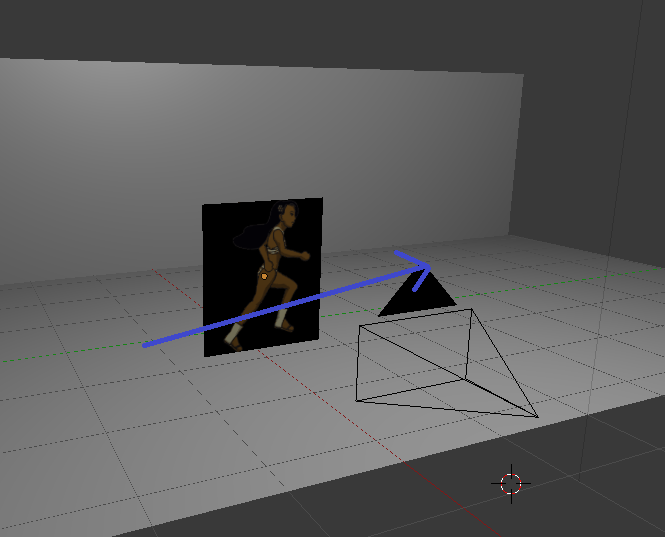
\includegraphics[width=0.7 \textwidth]{05TrabajoRealizado/01DocDiseno02/imagenes/camara01}}
   \subfigure[Seguimiento vertical.]{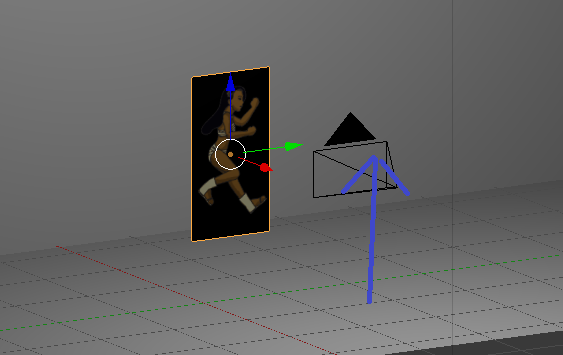
\includegraphics[width=0.7 \textwidth]{05TrabajoRealizado/01DocDiseno02/imagenes/camara02}}
  \caption{La cámara seguirá la posición del jugador en el eje x y y.}
  \label{fig:Camara}
\end{figure} 
 

\par
Por su parte, los controles del juego se establecieron como un conjunto de cuatro 
botones (Ver figura \ref{fig:GUI} ); cada uno con una acción específica a 
desempeñar: mover hacia la izquierda, mover hacia la derecha, disparar, hablar, 
saltar. Siendo periférico o el medio de interacción de los botones y el jugador 
la pantalla táctil del teléfono.  

\begin{figure}
				\centering
				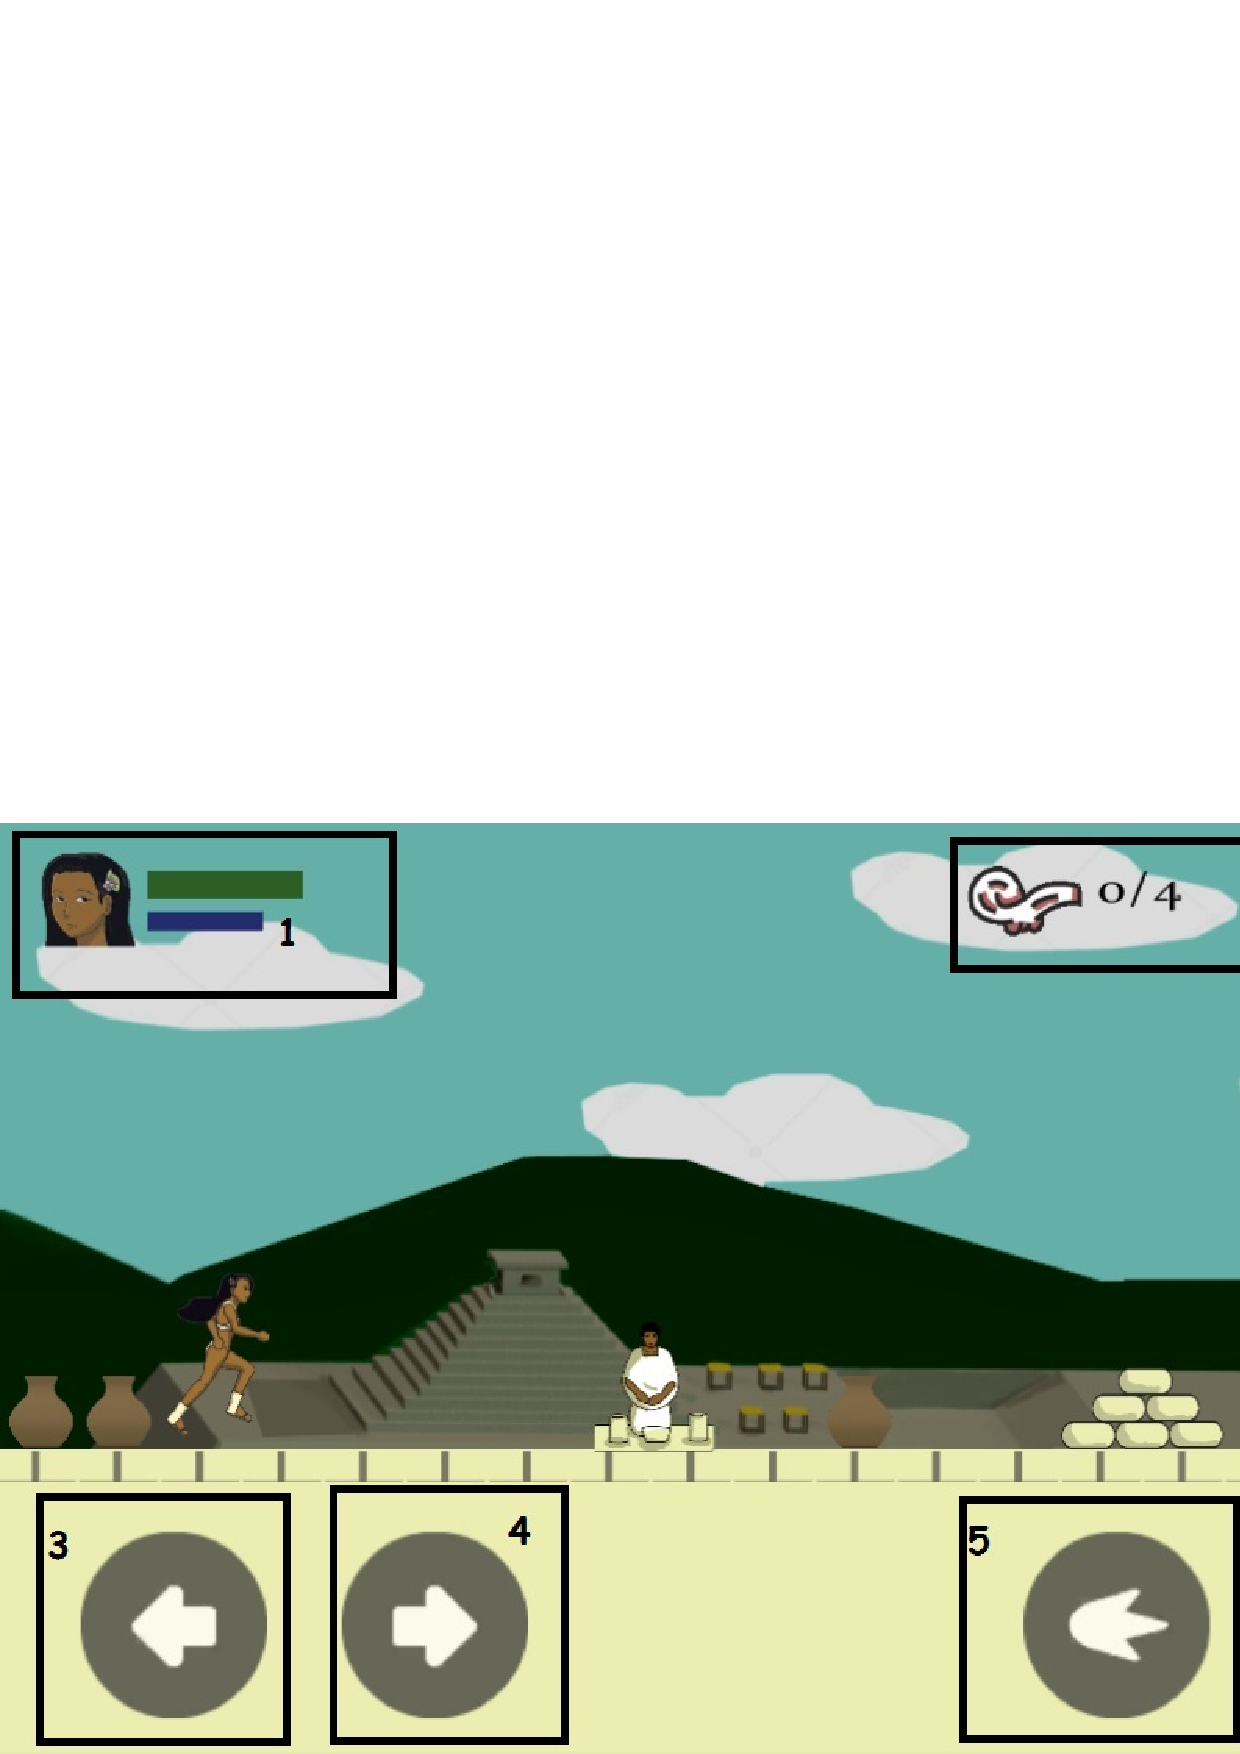
\includegraphics[height=0.3 \textheight]{05TrabajoRealizado/01DocDiseno02/imagenes/ControlCorrerDer}
				\caption{1 Información del personaje jugable, barra verde indicador 
				de la cantidad de vida, barra azul cantidad de tonalli. 2 Objetivos 
				del nivel o información útil. 3 Botón moverse izquierda. 4 Botón 
				moverse derecha. 5 Botón disparar tonalli. 6 Botón saltar.}
				\label{fig:GUI}
\end{figure}


\par
En cuanto al guardado y la carga, se propusieron dos tipos guardado y carga automática 
y guardado y carga de checkpoint; el primero guarda el progreso del jugador al 
completar el nivel y permite inicializar los niveles desbloqueados y el segundo 
se utiliza dentro de un nivel para guardar el progreso del jugador en el nivel 
en caso de que muera pueda iniciar desde el último checkpoint que tocó. 
Si el lector de este documento dese profundizar más en lo anteriormente dicho, 
se le recomienda consultar el Capítulo 5 del documento de diseño.
%===========================================
\subsection{Interfaces}\label{TraReaInterfaces}
Para la navegación dentro del juego, se diseñaron tres interfaces gráficas: 
La pantalla de inicio, Menú principal y el menú de selección de nivel. 
A continuación, se hará una breve descripción de la función principal de 
las interfaces:
\begin{itemize}
	\item\textbf{ Interfaz de inicio:} Presenta el logo del juego y la información 
	legal del mismo, sirve como pantalla de introducción al juego. Conecta con 
	la interfaz de menú principal (Ver figura \ref{fig:PInicio} ) .
	\item \textbf{Interfaz de menú principal:} Muestra la misma ilustración que la 
	pantalla de inicio, con la diferencia de que muestra dos botones en la parte 
	inferior izquierda de la pantalla. Con estos botones se puede empezar una nueva 
	partida o cargar una ya existente. Esta interfaz conecta a la cinemática de 
	inicio del juego si el jugador oprime el botón de empezar partida y confirma 
	que desea empezar una partida nueva o direcciona a la interfaz de menú de 
	selección de nivel, si el jugado oprime el botón de cargar partida y existe 
	un archivo con los datos del juego (Ver figura \ref{fig:PMenuP}).
	\item \textbf{Interfaz de Menú selección de nivel:} En esta interfaz el 
	jugador podrá elegir el nivel que desea jugar, siempre que lo haya desbloqueado 
	con anterioridad (Ver figura \ref{fig:SelNivel}).
\end{itemize}

\begin{figure}
  \centering
   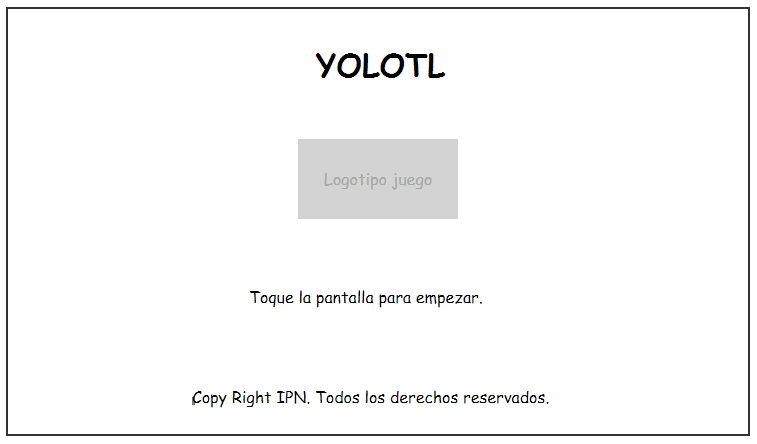
\includegraphics[width=0.6 \textwidth]{05TrabajoRealizado/01DocDiseno02/imagenes/interfaz00}
  \caption{Interfaz 1.0 Pantalla de inicio.}
  \label{fig:PInicio}
\end{figure} 


\begin{figure}
  \centering
   \subfigure[Menú principal] {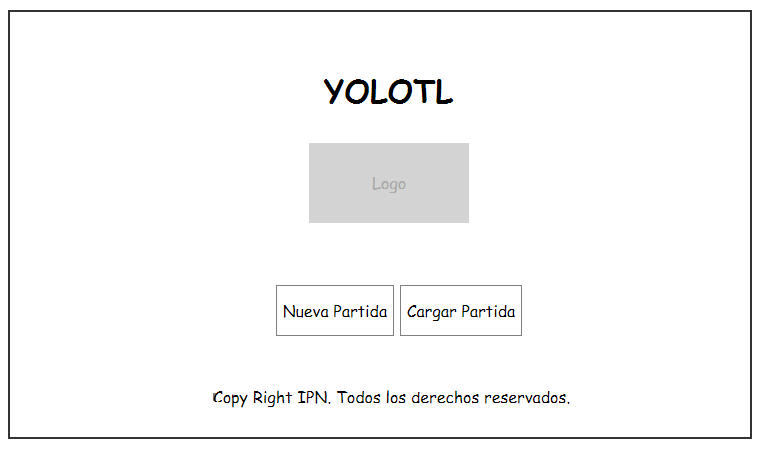
\includegraphics[width=0.6 \textwidth]{05TrabajoRealizado/01DocDiseno02/imagenes/interfaz01}}
   
 	\subfigure[Cuadro de dialogo para confirmar iniciar nueva partida.] {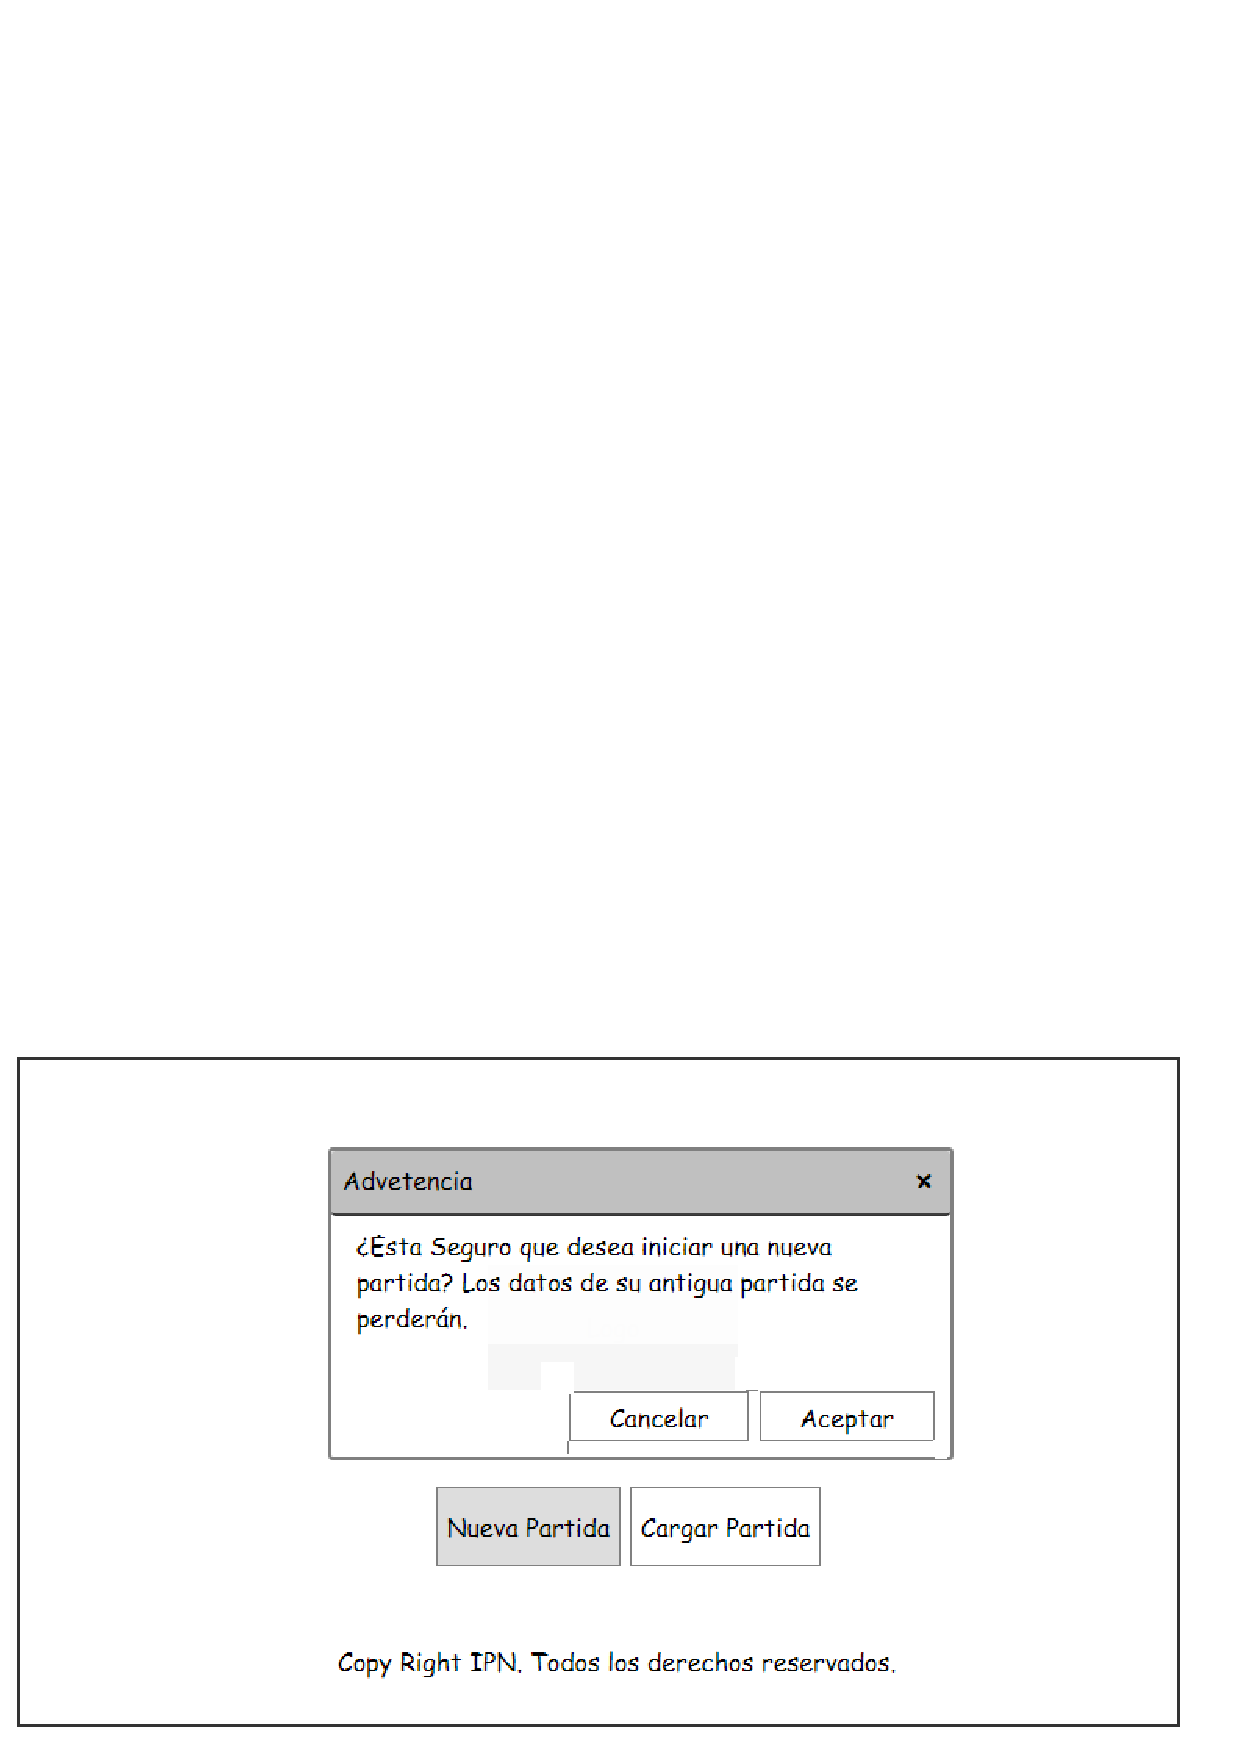
\includegraphics[width=0.6 \textwidth]{05TrabajoRealizado/01DocDiseno02/imagenes/interfaz01_02}}
 	
\subfigure[Cuadro de dialogo cuando no existen partidas que cargar.] {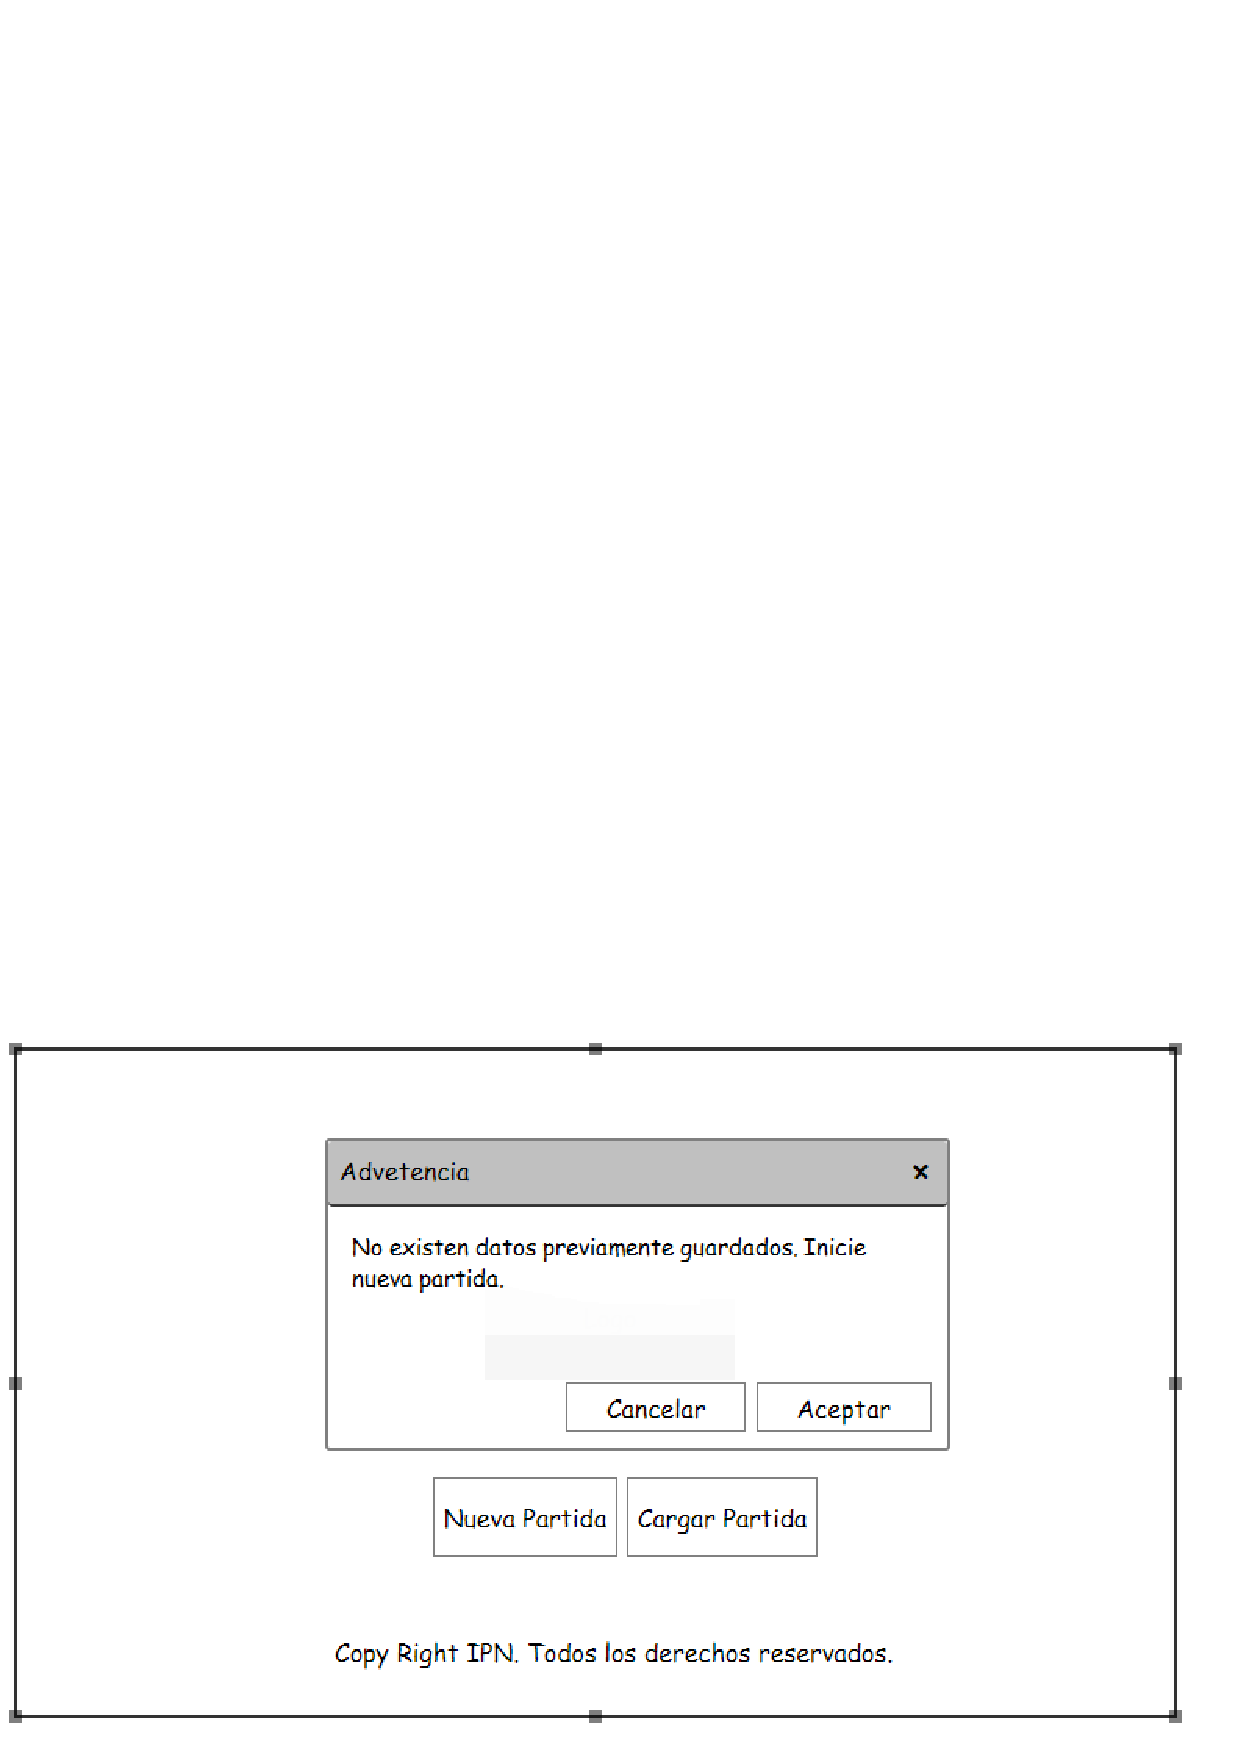
\includegraphics[width=0.6 \textwidth]{05TrabajoRealizado/01DocDiseno02/imagenes/interfaz01_03}}
  \caption{Interfaz 2.00 Menú principal.}
  \label{fig:PMenuP}
\end{figure} 


\begin{figure}
  \centering
   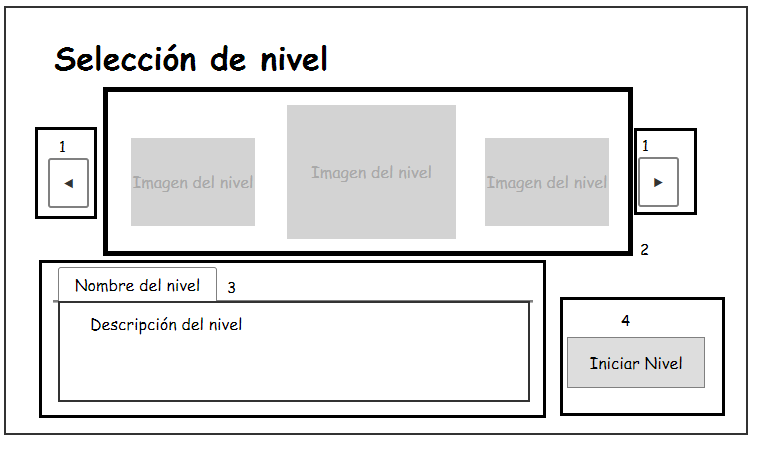
\includegraphics[width=0.6 \textwidth]{05TrabajoRealizado/01DocDiseno02/imagenes/interfaz02_01}
  \caption{Interfaz 2.00 Selección de nivel.1 botones que controlan el carrusel. 2 Carrusel. 3 Información del nivel seleccionado. 4 Botón Iniciar nivel.}
  \label{fig:SelNivel}
\end{figure}  
%===========================================
\subsection{Niveles.} \label{Niveles}
Yolotl es un juego compuesto por diez niveles: un nivel introductorio y los nueve 
niveles del inframundo.  Dado que la idea concepto del juego Yolotl lo situa en 
el Mictlán, la cantidad mínima esperados seria nueve; sin embargo, se tomó la 
decisión de incluir un nivel de introducción debido a los siguientes factores: 

\begin{itemize}
	\item Introducir al jugador a las mecánicas de juego básicas antes de lanzarlo 
	a un nivel más complicado.
	\item Situar el juego dentro de un contexto histórico real, permitiéndole al 
	jugador conocer sobre la sociedad Mexica de una manera en la que el jugador 
	pueda ser participe de este contexto histórico.
	\item Seguir una estructura narrativa básica en la que se presente la vida 
	cotidiana del héroe antes del llamado a la aventura \cite{RefHeroe}.
\end{itemize}

Usualmente, en el juego de Yolotl, un nivel está compuesto de dos secciones: una 
sección de obstáculos y plataformas en donde cumplirá un objetivo propio del nivel 
y otra donde el jugador se enfrentará al enemigo jefe del nivel. A excepción 
del primero y ultimo nivel el resto de los niveles siguen esa estructura. En el 
caso del primer nivel sigue la división de las dos secciones, con la diferencia 
de que no existe un enemigo jefe a vencer en la segunda sección del nivel; 
mientras que en el último nivel existe una única sección en donde el jugador 
se enfrentará a las diferentes transformaciones del jefe final.
\\
\par
La progresión entre niveles es lineal (Ver figura \ref{fig:ProgreNiveles}), 
por lo que no se puede acceder al nivel determinado sin antes haber completado 
a su predecesor; siendo el primer nivel, el que se encuentra disponible de manera 
estándar al empezar una nueva partida. Un nivel se da completado únicamente 
hasta que se ha derrotado al enemigo jefe del nivel; salvo por el primer nivel, 
el cual se considera terminado una vez que el jugador obtiene el arma de la 
protagonista. Cuando el jugador completa un nivel, además de desbloquear el 
siguiente nivel, el jugador podrá ver determinadas cinemáticas con las que podrá 
seguir la historia del juego y obtiene mejoras sobre alguno de los atributos del 
personaje.
\\
\par
En la tabla se encuentra información referente a cada nivel tal como los 
objetivos a cumplir, el enemigo a vencer, lo que se obtiene al completar el nivel.

%%============== PROGRECION DE NIVELES ==============
\begin{figure}
  \centering
   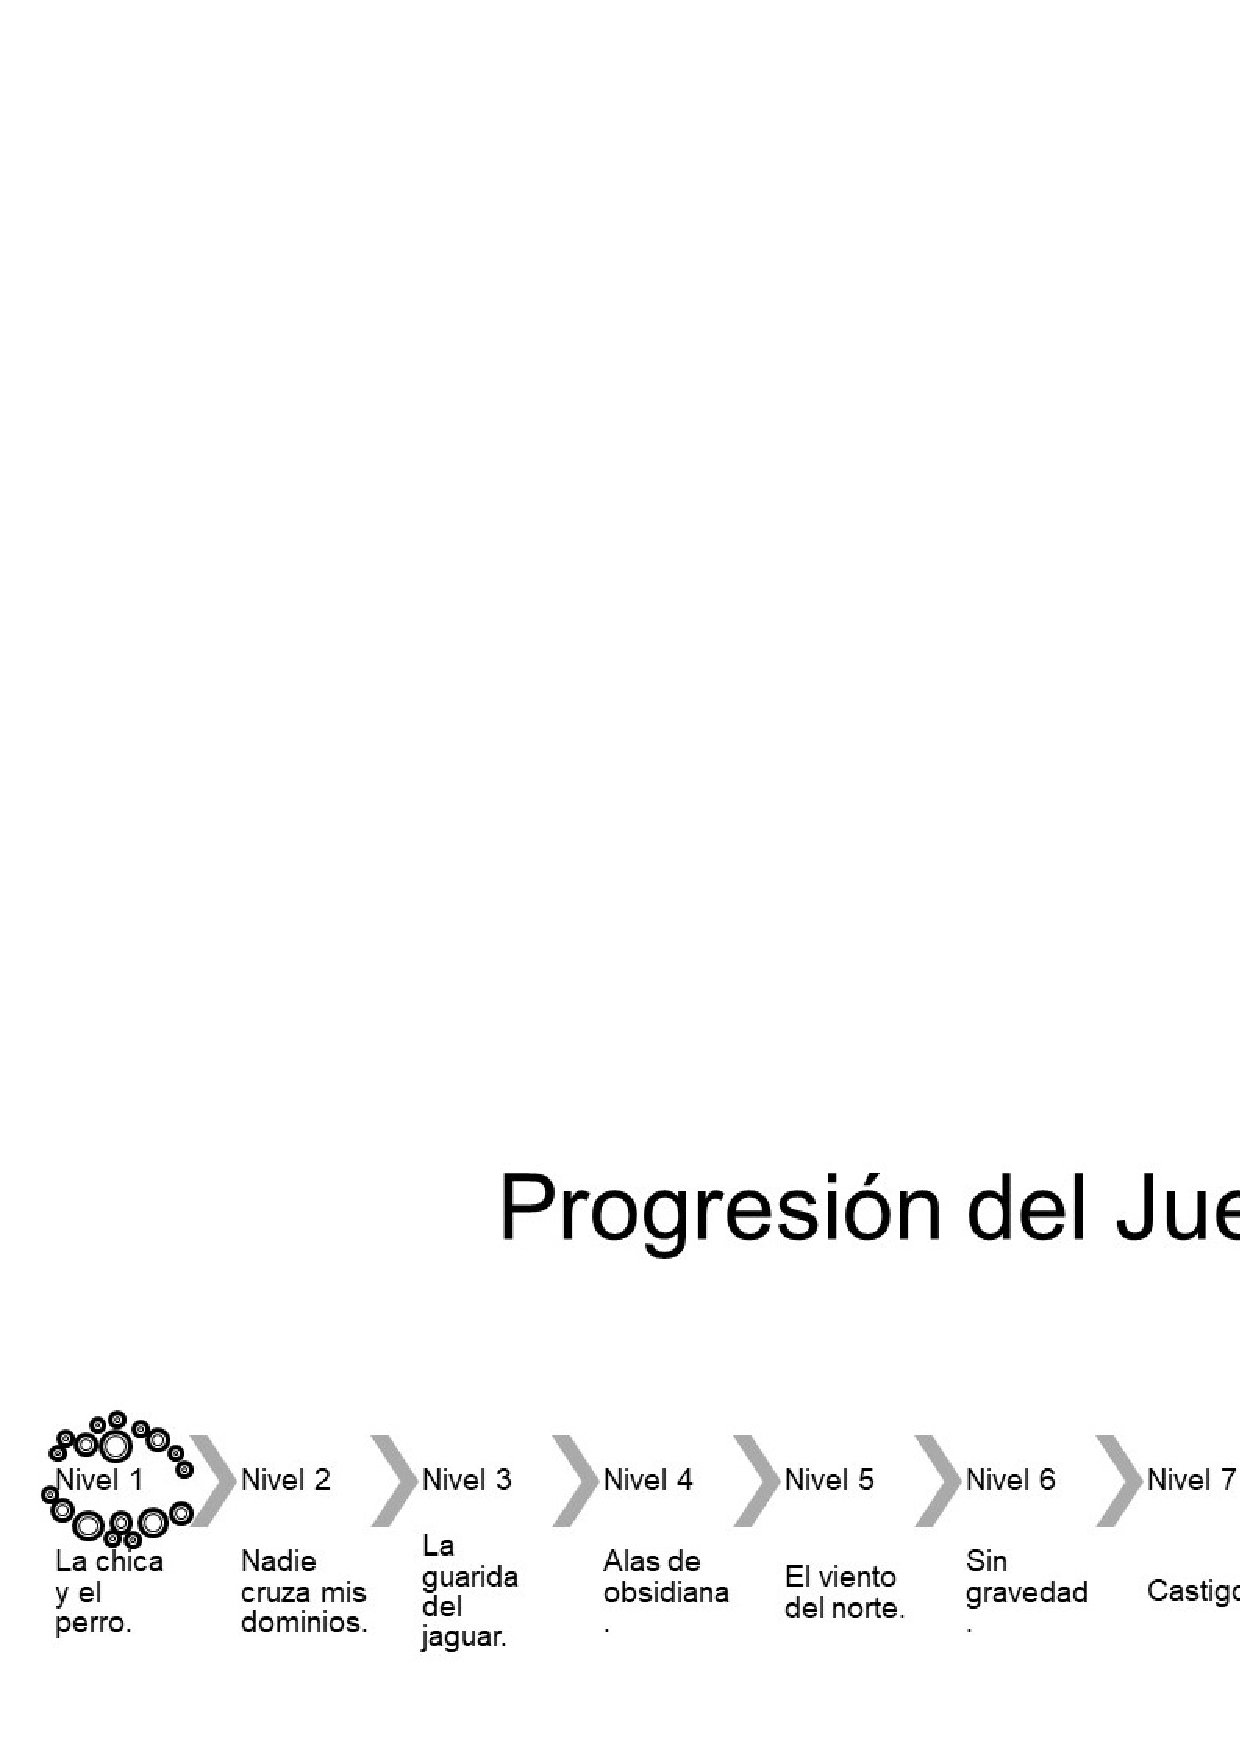
\includegraphics[width=0.8 \textwidth]{05TrabajoRealizado/01DocDiseno02/imagenes/ProgresJuego}
  \caption{Progresión del juego}
  \label{fig:ProgreNiveles}
\end{figure} 

%%============== TABLA DE NIVELES =============
%\begin{table}
	\begin{longtable}[c]{ | m{3.75cm} | m{3.75cm}| m{3.75cm} | m{3.75cm}|} 
		%\endhead		
		%\endfirsthead
		%\endlastfoot
		%\hline
		\rowcolor{cyan} Nivel.& Objetivo & Zona de plataformas	Enemigo jefe & Progreso obtenido. \\ 
		\hline
		%-------------------------------
		Nivel 1 “La chica y el perro”. & 
		Hablar con al menos cuatro ciudadanos.
			\par 
			Interactuar con Xólotl.
			\par 
			Obtener la caracola.&
		Sin enemigo jefe.&
		 Nivel 1.
			\par 
			Cinemática 3.
			\par 
			Cinemática 4.
			\par 
			Habilidad de disparo.		 
		 \\ 
		\hline
		%-------------------------------
		Nivel 2 “Nadie cruza mis dominios”. & 
		Atravesar el rio evitando tocar a los Xoloitzcuintles, por cada Xoloitzcuintles tocado incrementara el poder de Xochitónal. &
		Xochitónal. &
		Mejora en la cantidad de vida de Malinalli.
			\par 
			Cinemática 6.
			\par 
			Cinemática 7.
			\par 
			Cinemática 8.
			\par 
			Cinemática 9.
			\par 
			Cinemática 10.
			\par 
			Nivel 3.		 
		 \\ 
		\hline
		%-------------------------------
		Nivel 3 “La guarida del jaguar”. & 
		Llegar a la guarida de Tepeyóllotl. &
		Tepeyóllotl. &
		Mejora en la cantidad de Tonalli de Malinalli.
			\par 
			Cinemática 12.
			\par
			Cinemática 13.
			\par 
			Cinemática 14.
			\par
			Nivel 4.		 
		 \\ 
		\hline
		%-------------------------------
		Nivel 4 “Alas de obsidiana”. & 
			Encontrar el camino correcto hacia la guarida de Itzpapálotl.
			\par
			Encontrar las tres llaves que abren la puerta de la guarida de Itzpapálotl.&
		Itzpapálotl. &
			 Mejora en la cantidad de vida de Malinalli.
			 \par
			 Cinemática 16.
			 \par
			 Cinemática 17.
			 \par
			 Cinemática 18.
			 \par
			 Cinemática 19.
			 \par
			 Cinemática 20.
			 \par
			 Cinemática 21.
			 \par
			 Cinemática 22.
			 \par
			 Nivel 5.		 
		 \\ 
		\hline
		%-------------------------------
		Nivel 5 “El viento del norte”. & 
		Llegar a la guarida Mictlecayotl.&
		Mictlecayotl. &
		Mejora en la cantidad de Tonalli de Malinalli.
		\par
		Cinemática 24.
		\par
		Cinemática 25.
		\par
		Cinemática 26.
		\par
		Cinemática 27.
		\par
		Nivel 6.		 
		 \\ 
		\hline
		%-------------------------------
		Nivel 6 “Sin gravedad”. & 
		Llegar a la guarida Tlazoltéotl &
		Tlazoltéotl. &
		Mejora en la cantidad de vida de Malinalli.
		\par
		Cinemática 29.
		\par
		Cinemática 30.
		\par
		Cinemática 31.
		\par
		 Nivel 7.		 
		 \\ 
		\hline
		%-------------------------------
		Nivel 7 “Castigo”. & 
		Llegar a la guardia Itztlacoliuhqui. &
		Itztlacoliuhqui. &
		Mejora en la cantidad de Tonalli de Malinalli.
		\par
		Cinemática 33.
		\par
		Cinemática 34.
		\par
		Cinemática 35.
		\par
		Nivel 8.		 
		 \\ 
		\hline
		%-------------------------------
		Nivel 8 “La última batalla del jaguar”. & 
		Llegar a la guarida de Tepeyóllotl.&
		Tepeyóllotl. &
		Mejora en la cantidad de vida de Malinalli.
		\par		
		Cinemática 37.
		\par
		Cinemática 38.
		\par
		Cinemática 39.
		\par
		Nivel 9.		 
		 \\ 
		\hline
		%-------------------------------
		Nivel 9 “El último caballero del rey”. & 
		Superar la zona de Tula.
		\par
		Superar la zona de Oluta.&
		Nexoxcho. &
		Mejora en la cantidad de Tonalli de Malinalli.
		\par		
		Cinemática 44.
		\par
		Cinemática 45.
		\par
		Cinemática 46.
		\par
		Nivel 10. 
		 \\ 
		\hline
		%-------------------------------
		Nivel 10 “El rey del Mictlán”. & 
		Sin objetivos &
		Mictlantecutli. &
		Cinemática 47.
		\par		
		Juego terminado. 
		 \\ 
		\hline
	\end{longtable}

	%\caption{Información de los niveles.}
	%\label{Tab:Niveles}
%\end{table}
%===========================================
\subsection{Obstáculos}
De manera particular, para el proyecto Yolotl, se entiende por obstáculos a aquellos objetos dentro de un nivel que dificultan el avance continuo del jugado o que faciliten el fallo del jugador.
\\
\par
A diferencia de los personajes, la metodología huddle no maneja una plantilla para documentar estos objetos, por lo que se propuso una plantilla propia. Los campos de la plantilla son:
	\begin{itemize}
		\item Nombre del obstáculo.
		\item Descripción: Este campo describe tanto físicamente el objeto como su comportamiento e interacción con el jugador. 
		\item Esquema: Imagen de apoyo que facilita la comprensión de la descripción. 
	\end{itemize}
En total se definieron alrededor de 11 obstáculos, mismos que se podrán encontrar repartidos a lo largo de los niveles del juego. Algunos obstáculos serán exclusivos de un nivel mientras que otros se podrán encontrar en todos los niveles.
 \\
 \par
 A continuación se listarán los obstáculos del juego:
 	\begin{itemize}
 		\item Caja.
 		\item Sacos de cacao.
 		\item Plataforma móvil.
 		\item Plataforma que cae.
 		\item Plataforma que desaparece.
 		\item Estalagmitas.
 		\item Viento temporal.
 		\item Piedras filosas.
 		\item Piso congelado.
 		\item Bolas de nieve.
 		\item Lluvia de flechas.
 	\end{itemize}
%===========================================
\subsection{Ambientación}
	Para garantizar la inmersión del jugador, el videojuego se vale de diferentes
	 elementos multimedia. Estos elementos son la música de fondo (BGM, pos sus 
	 siglas en inglés), los efectos de sonido (SFX, por sus siglas en inglés) y  
	 efectos espaciales (FX, por su siglas en inglés).
\\
\par	
	Huddle maneja un aparatado para incluir este tipo de elementos dentro de la 
	documentación del juego; sin embargo, no incluye ninguna guía sobre como debería 
	de redactarse las descripciones de BGM y SFX; en consecuencia estos elementos 
	fueron documentados escribiendo el nombre de sonido o música, seguido de una 
	breve descripción del mismo.   
\\
\par
Durante la redacción de este aparatado se detectó que existían dos secciones para 
documentar BGM y SFX, con la diferencia de que en una los términos se encontraban 
escritos en sus siglas en inglés y en el otro apartado se encontraba en español, 
por lo que se eliminó el apartado en español. Luego de que se detectara esta 
duplicación de apartados, se descubrió que no existía ningún apartado para documentar 
los FX, seguido de esto se creo dicho apartado. En cuanto a la documentación de FX, 
se siguió la misma estructura que con BGM y SFX: escribir el nombre de FX y 
describirlo para dar una idea de como se vería en el nivel y bajo que interacciones 
se activaría. 
%===========================================
\subsection{Argumento del videojuego}
Huddle maneja un apartado llamado \textbf{Guión} para documentar de manera detallada 
la historia del videojuego. No obstante, al igual que como sucede con algunos de 
los apartados ya descritos, Huddle no proporciona una plantilla para documentarlo. 
Ante la falta de una plantilla para documentar el argumento y ante la existencia 
de cinemáticas dentro de los niveles y fuera de estos, se decidió que el argumento 
del juego se documentaría como una animación. Contando así con tres guiones:
	\begin{itemize}
		\item \textbf{Guión literario}:Este guión es parecido a un guión teatral. 
		Por medio de escenas va desarrollando la historia, mostrando la secuencia 
		de diálogos que entablan los personajes participes en el argumento. Para 
		el caso particular del videojuego Yolotl, las escenas recibe el nombre de 
		cinemáticas. Cada cinemática se documentara bajo la siguiente plantilla:
			\begin{itemize}
				\item Numero de la cinemática seguido del nombre la locación donde 
				acontece ésta; en caso de que la escena suceda en el interior de 
				alguna edificación se pondrá seguido del nombre de la locación el 
				prefijo int, en caso de suceder en el exterior se colocará el 
				prefijo ext.
				\item Relación con los nombres de todos los personajes que participan 
				en la escena.
				\item Breve descripción de la locación.
				\item Secuencia de diálogos. Cada diálogo va precedido por el nombre 
				de personaje que lo dice, el nombre del personaje debe de ir en 
				mayúsculas y subrayado. 
			\end{itemize}
			\item Storyboard: El storyboard es una secuencia de imágenes que narran 
			de manera visual la historia. Cada imagen va comentada de tecnicismos 
			que faciliten la descripción de acciones (tales como el desplazamiento 
			de la cámara, movimientos de personajes, intención del personaje en 
			decir un diálogo, etc.) \cite{RefStoyBoard}.  			 
	\end{itemize}


	\section{Análisis del juego}
En esta sección se presenta el analisis que se realizo del juego con base en el 
documento de diseño descrito en el apartado \ref{docDisenio}.Primeramente se 
describe al usuario que se identificó y las acciones que éste puede realizar 
dentro del juego; en segundo lugar se habla de las clases que componen el juego, 
describiéndose lo tres tipos de clases en el que se clasificaron, para 
posteriormente listar que clases pertenecen a cada un de los tipos. Para finalizar 
esta sección se describe la comunicación entre clases para tres procesos que 
realiza el juego. 

	\subsection{Usuario del sistema}
	Tomando como referencia el documento de diseño se identificó el siguiente actor:
	\begin{itemize}
		\item \textbf{Jugador:} Es el usuario del sistema y quien interactua con
		el mismo. Dentro del sistema el jugador puede: 
			\begin{itemize}
				\item Empezar una partida nueva.	
				\item Cargar una partida ya existente.
				\item Elegir un nivel para jugar.  
				\item Jugar.
				\item Pausar Nivel.
				\item Reanudar nivel pausado.
				\item Ver cinemática.
			\end{itemize}			   
	\end{itemize}	
	
	\subsection{Clases del juegos} \label{ClasesJuego}
	A partir del documento de diseño se identificaron al rededor de (); estas 
	clases se dividen en tres grupos:
		\begin{itemize}
			\item \textbf{Controladores:} Clases encargadas de controlar la gestión de 
			la partida y la navegación dentro del juego. Estas clases regulan las acciones 
			de las clases actoras y desencadenan determinados eventos dentro del juego
			dependiendo de las acciones del Jugador y de las reglas de los niveles.
			
			\item \textbf{Actores:} Son las clases que modelan a los enemigos, obstáculos,
			\textit{checkpoints} y el jugador.
			 
			 \item \textbf{Auxiliares:} Son todas aquellas clases que ayudan a los controladores
			 a cumplir con su funcionalidad al permitirle a los controladores obtener datos 
			 para inicializar valores o garantizar las transiciones entre interfaces.
		\end{itemize}
		
	\subsubsection{Clases controladoras} \label{ClaseCtrl}
		\begin{itemize}
			\item \textbf{PrincipalMenuCtrl:} Esta clase se encarga de la funcionalidad del menú 
			principal. Esta clase esta a cargo de:
			\begin{itemize}
				\item Empezar nueva partida.
				\item Cargar nueva partida.
				\item Mostrar mensajes de confirmación antes de proceder con cambios 
				irreversibles a los datos de partida.
				\item Mostrar mensaje de aviso en caso de no encontrar exista una partida 
				guardada. 
			\end{itemize}
			%=======================================
			\item \textbf{SelectLevelMenu:} Esta clase controla la funcionalidad del menú de 
			selección nivel. Esta clase realiza:
			\begin{itemize}
				\item Habilitar solo los niveles y cinemáticas que el jugador haya 
				desbloqueado.
				\item No permitir que el jugador pueda acceder a niveles o cinemáticas 
				que el jugador no haya desbloqueado.
				\item Direccionar al jugador al nivel o a la cinemática que seleccionó.
			\end{itemize}
			%=======================================
			\item \textbf{GameDataCtrl:} Esta clase controla el archivo de los datos de 
			partida, este archivo sera de formato binario, este formato es un tipo de 
			archivo que propio de Unity y permite proteger los datos de las partidas evitando
			que estos puedan ser modificados por el jugador, garantizando así la integridad 
			de la información. Está ligada a la mayoría de los controladores pues de ella depende 
			 guardar y cargar el progreso del jugador para inicializar valores como: la 
			 vida del jugador, su cantidad de \textit{Tonalli}, los niveles disponibles, etc. 
			 Dentro de su funcionalidad está: 
			\begin{itemize}
				\item Verificar la existencia del archivo de datos de partida.
				\item Crear un archivo de datos de partida.
				\item Leer los datos del archivo de datos de partida.
				\item Escribir datos en el archivo de partida.
			\end{itemize}
			%=======================================
			\item \textbf{DialogueCtrl:} Esta clase se encarga del despliegue de diálogos
			en las cinemáticas y dentro de los niveles. Esta clase realiza las siguientes 
			actividades:
			\begin{itemize}
				\item Iniciar el despliegue de diálogos.
				\item Mostrar el dialogo siguiente.
				\item Finalizar el despliegue diálogos. 
			\end{itemize}	
			%=======================================
			\item \textbf{TalkedCharactersCtrl:} Esta clase asigna una instancia de la 
			clase \textit{Dialogue} a cada una de las instancias de la clase 
			\textit{TalkedCharacter}.
			%=======================================
			\item \textbf{CutsceneCtrl:} Esta clase se encarga de vincular el despliegue 
			de diálogos con las animaciones de las cinemáticas. Esta clase tiene diversas 
			clases hijas que heredan su funcionalidad de vinculación de diálogos y animación 
			incorporando las consideraciones necesarias para el control de cada cinemática.
			%=======================================
			\item \textbf{AudioCtrl:} Esta clase esta a a cargo de generar los sonidos de \textit{SFX} 
			dentro del juego utilizando la posición del jugador o de los enemigos. 
			%=======================================
			\item \textbf{LevelCtrl:} Esta clase controla el nivel que el jugador esta 
			jugando. Esta clase realiza las siguientes acciones:
			\begin{itemize}
				\item Inicializar los atributos de la clase \textit{Player}.
				\item Verificar que el jugador este vivo.
				\item Actualizar la barra de vida del jugador.
				\item Actualizar la barra de cantidad \textit{Tonalli}.
				\item Pausar el juego.
				\item Reanudar juego pausado. 
			\end{itemize}
			Esta clase tiene clases hijas que se encargan de:
				\begin{itemize}
					\item Verificar que se cumplan los objetivos específicos del nivel.
					\item Actualizar los objetivos del nivel.
					\item Actualizar los contadores de los objetivos.
					\item Guardar el progreso obtenido en el nivel.
					\item Inicializar los valores del jugador con base al \textit{checkpoint} activo. 
				\end{itemize}
			%=======================================
			\item \textbf{CameraCtrl:} Esta clase controla el desplazamiento de la cámara.
			%=======================================
			\item \textbf{MobileUICtrl:} Esta clase se encarga de comunicar al jugador 
			con la clase \textit{Player}. Es a través de esta clase que el jugador puede controlar 
			al personaje jugable. Esta clase le permite al jugador:
			\begin{itemize}
				\item Mover al personaje jugable a la derecha.
				\item Mover al personaje a la izquierda.
				\item Detener el movimiento del jugador.
				\item Actualizar la barra de cantidad \textit{Tonalli}.
				\item Pausar el juego.
				\item Reanudar juego pausado. 
			\end{itemize}
			%=======================================
			\item \textbf{ArrowCreator:} Esta clase crea objetos que instancían al prefab "Arrow".								
		\end{itemize}				  
	\subsubsection{Clases Actores}
A continuación se listan las clases actores: 
		\begin{itemize}
			\item \textbf{Player:} Esta clase se encarga de las acciones del personaje 
			jugable, actualizar sus estados y gestionar el valor de sus atributos. 
			Esta clase esta a cargo de:
			\begin{itemize}
				\item Mover al personaje jugable de manera horizontal.
				\item Controlar la maquina de estados de las animaciones del personaje 
				jugable.
				\item Detectar las colisiones del personaje jugable.
				\item Actualizar la cantidad de vida al recibir daño.
				\item Realizar disparo de \textit{Tonalli}.
				\item Actualizar la cantidad de \textit{Tonalli} al efectuar un disparo.  
				\item Saltar. 
			\end{itemize}
			%=======================================
			\item \textbf{TalkedCharacter:} Esta clase modela el funcionamiento de un
			ciudadano con el que el jugador debe interactuar en el nivel 1.
			Esta clase esta a cargo de:
			\begin{itemize}
				\item Mostrar un ícono de diálogo para indicarle al jugador que debe de 
				interactuar con éste.
				\item Ocultar el ícono de diálogo.
				\item Indicarle a la clase DialogueCtrl que se inicia un diálogo.  
			\end{itemize}
			%=======================================
			\item \textbf{DroppingPlatform:} Esta clase modela el funcionamiento 
			del obstáculo Plataforma que cae, por lo que al hacer contacto con un objeto de 
			la clase \textit{GroundCollisionCtrl} el objeto que instancie esta clase 
			empezará a caer despues de \textit{n} segundos. 
			%=======================================
			\item \textbf{MovingPlatform:} Esta clase modela el funcionamiento 
			del obstáculo Plataforma que móvil. Haciendo uso de dos posiciones: A y B, el 
			objeto que instancia esta clase se mueve de manera cíclica de la posición A a 
			la B y de la B a la A. 
			%=======================================
			\item \textbf{DisappearingPlatform:} Esta clase modela el funcionamiento 
			del obstáculo Plataforma que desaparece, esta clase hace que el objeto que la 
			instancie aparezca y desaparezca de manera cíclica, activando y desactivando 
			los colisionadores del objeto. 
			%=======================================
			\item \textbf{Stalagmite:} Esta clase modela el comportamiento del obstáculo 
			estalagmita. Esta clase hace que el objeto que la instancie caiga cuando 
			detecte que el jugador se posiciona por debajo de este objeto.    
			%=======================================
			\item \textbf{PushingObstacle:} Esta clase modela el comportamiento de dos 
			obstáculos: viento temporal y bolas de nieve. Haciendo uso de una posición, la
			clase determina hacia que dirección debe de incrementar su dimensión y el tamaño 
			de su colisionador.      
			%=======================================	
			\item \textbf{Arrow:} Clase que produce un movimiento vertical descendente al 
			objeto que la instancia.   
			%=======================================
			\item \textbf{\textit{Enemy}:} Esta clase modela el comportamiento común que 
			tienen los enemigos de tipo normal y los de tipo jefe. De esta clase heredan 
			su funcionamiento las clase \textit{NormalEnemy} y \textit{BossEnemy}.Esta 
			clase se encarga de:  
			\begin{itemize}
				\item Controlar las transiciones de la maquina de estados que controla las 
				animaciones del enemigo.
				\item Gestiona la detección de colisiones del enemigo.
				\item Actualizar la cantidad de vida del Enemigo.
			\end{itemize}
			%=======================================
			\item \textbf{\textit{NormalEnemy}:} Esta clase modela el comportamiento común que 
			tienen los enemigos de tipo normal. Esta clase hereda su funcionamiento de la clase
			 \textit{Enemy}. La clase NormalEnemy hereda su funcionalidad a las clases 
			\textit{ Jaguar, Bird, Armadillo, PurpleGost} y \textit{RedGost}.Esta 
			clase se encarga de:  
			\begin{itemize}
				\item Controlar el patrón de movimiento de los enemigos de tipo 
				normal.
				\item  Verificar la cercanía que tiene el enemigo normal con otros objetos, 
				obstáculos y enemigos para ajustar su rango de acción y evitar que interfiera con el 
				funcionamiento de otro objeto.
			\end{itemize}					
			%=======================================
			\item \textbf{\textit{Jaguar}:} Esta clase modela el comportamiento del enemigo jaguar 
			(Consultar la ficha de personaje en la Sección de personajes en el documento de diseño). 
			Esta clase hereda su funcionamiento de la clase \textit{NormalEnemy}. Esta 
			clase se encarga de:  
			\begin{itemize}
				\item Sincronizar el desplazamiento del jaguar con su maquina de estados para que modele
				el patrón de ataque del jaguar. 
			\end{itemize}
			%=======================================
			\item \textbf{\textit{Bird}:} Esta clase modela el comportamiento de dos personajes de tipo
			normal: Chara enana y Zopilote (Consultar la ficha de personaje en la Sección de personajes en 
			el documento de diseño). Esta clase hereda su funcionamiento de la clase 
			\textit{NormalEnemy}. Esta clase se encarga de:  
			\begin{itemize}
				\item Sincronizar el desplazamiento del ave con su maquina de estados para que modele
				el patrón de ataque de Chara enana y del zopilote. 
			\end{itemize}
			%=======================================
			\item \textbf{\textit{Armadillo}:} Esta clase modela el comportamiento del personaje 
			armadillo (Consultar la ficha de personaje en la Sección de personajes en 
			el documento de diseño). Esta clase hereda su funcionamiento de la clase 
			\textit{NormalEnemy}. Esta clase se encarga de:  
			\begin{itemize}
				\item Sincronizar el desplazamiento del jaguar con su maquina de estados para que modele
				el patrón de ataque del armadillo. 
			\end{itemize}
			%=======================================
			\item \textbf{\textit{PurpleGost}:} Esta clase modela el comportamiento del personaje 
			fantasma purpura (Consultar la ficha de personaje en la Sección de personajes en 
			el documento de diseño). Esta clase hereda su funcionamiento de la clase 
			\textit{NormalEnemy}. Esta clase se encarga de:  
			\begin{itemize}
				\item Sincronizar el desplazamiento del jaguar con su maquina de estados para que modele
				el patrón de ataque del fantasma purpura. 
			\end{itemize}
			
			%=======================================
			\item \textbf{\textit{RedGost}:} Esta clase modela el comportamiento del personaje 
			fantasma rojo (Consultar la ficha de personaje en la Sección de personajes en 
			el documento de diseño). Esta clase hereda su funcionamiento de la clase 
			\textit{NormalEnemy}. Esta clase se encarga de:  
			\begin{itemize}
				\item Sincronizar el desplazamiento del jaguar con su maquina de estados para que modele
				el patrón de ataque del fantasma rojo.
				\item Instanciar el objeto ShootEnemy. 
			\end{itemize}
			%=======================================
			\item \textbf{\textit{BossEnemy}:} Esta clase modela el comportamiento común que 
			tienen los enemigos de tipo ¿jefe. Esta clase hereda su funcionamiento de 
			la clase \textit{Enemy}. La clase BosslEnemy hereda su funcionalidad a las clases 
			\textit{ Xochitonal, Tepeyollotl,Itzpapalotl, Mictlecayotl, Tlazolteotl, 
			Itztlacoliuhqui, Nexoxcho, MictlantecutliPhase01, MictlantecutliPhase02} 
			y \textit{MictlantecutliPhase03}.Esta clase se encarga de:  
			\begin{itemize}
				\item Controlar el patrón de movimiento de los enemigos de tipo 
				jefe.
				\item  Verificar la cercanía que tiene el enemigo tipo jefe con el jugador 
				y con los limites del escenario.
			\end{itemize}	
			%=======================================
			\item \textbf{\textit{Xochitonal}:} Esta clase modela el comportamiento del personaje 
			\textit{Xochitónal} (Consultar la ficha de personaje en la Sección de personajes en 
			el documento de diseño). Esta clase hereda su funcionamiento de la clase 
			\textit{BossEnemy}. Esta clase se encarga de:  
			\begin{itemize}
				\item Sincronizar el desplazamiento del \textit{Xochitónal} con su maquina 
				de estados para que modele el patrón de \textit{Xochitónal}.
				\item Toma decisiones en cuanto a los ataques a realizar basándose en su 
				nivel de vida.
			\end{itemize}
			%=======================================
			\item \textbf{\textit{Tepeyollotl}:} Esta clase modela el comportamiento del personaje 
			\textit{Tepeyóllotl} (Consultar la ficha de personaje en la Sección de personajes en 
			el documento de diseño). Esta clase hereda su funcionamiento de la clase 
			\textit{BossEnemy}. Esta clase se encarga de:  
			\begin{itemize}
				\item Sincronizar el desplazamiento del \textit{Tepeyóllotl} con su maquina 
				de estados para que modele el patrón de \textit{Tepeyóllotl}.
				\item Toma decisiones en cuanto a los ataques a realizar basándose en su 
				nivel de vida.
			\end{itemize}
			%=======================================
			\item \textbf{\textit{Itzpapalotl}:} Esta clase modela el comportamiento del personaje 
			\textit{Itzpápalotl} (Consultar la ficha de personaje en la Sección de personajes en 
			el documento de diseño). Esta clase hereda su funcionamiento de la clase 
			\textit{BossEnemy}. Esta clase se encarga de:  
			\begin{itemize}
				\item Sincronizar el desplazamiento del \textit{Itzpápalotl} con su maquina 
				de estados para que modele el patrón de \textit{Itzpápalotl}.
				\item Toma decisiones en cuanto a los ataques a realizar basándose en su 
				nivel de vida.
			\end{itemize}
			%=======================================
			\item \textbf{\textit{Mictlecayotl}:} Esta clase modela el comportamiento del personaje 
			\textit{Mictlecayotl} (Consultar la ficha de personaje en la Sección de personajes en 
			el documento de diseño). Esta clase hereda su funcionamiento de la clase 
			\textit{BossEnemy}. Esta clase se encarga de:  
			\begin{itemize}
				\item Sincronizar el desplazamiento del \textit{Mictlecayotl} con su máquina 
				de estados para que modele el patrón de \textit{Mictlecayotl}.
				\item Toma decisiones en cuanto a los ataques a realizar basándose en su 
				nivel de vida.
			\end{itemize}
			%=======================================
			\item \textbf{\textit{Tlazolteotl}:} Esta clase modela el comportamiento del personaje 
			\textit{Tlazoltéotl} (Consultar la ficha de personaje en la Sección de personajes en 
			el documento de diseño). Esta clase hereda su funcionamiento de la clase 
			\textit{BossEnemy}. Esta clase se encarga de:  
			\begin{itemize}
				\item Sincronizar el desplazamiento del \textit{Tlazoltéotl} con su maquina 
				de estados para que modele el patrón de \textit{Tlazoltéotl}.
				\item Toma decisiones en cuanto a los ataques a realizar basándose en su 
				nivel de vida.
			\end{itemize}
			%=======================================
			\item \textbf{\textit{Itztlacoliuhqui}:} Esta clase modela el comportamiento del personaje 
			\textit{Itztlacoliuhqui} (Consultar la ficha de personaje en la Sección de personajes en 
			el documento de diseño). Esta clase hereda su funcionamiento de la clase 
			\textit{BossEnemy}. Esta clase se encarga de:  
			\begin{itemize}
				\item Sincronizar el desplazamiento del \textit{Itztlacoliuhqui} con su máquina 
				de estados para que modele el patrón de \textit{Itztlacoliuhqui}.
				\item Toma decisiones en cuanto a los ataques a realizar basándose en su 
				nivel de vida.
			\end{itemize}
			%=======================================
			\item \textbf{\textit{Nexoxcho}:} Esta clase modela el comportamiento del personaje 
			\textit{Nexoxcho} (Consultar la ficha de personaje en la Sección de personajes en 
			el documento de diseño). Esta clase hereda su funcionamiento de la clase 
			\textit{BossEnemy}. Esta clase se encarga de:  
			\begin{itemize}
				\item Sincronizar el desplazamiento del \textit{Nexoxcho} con su maquina 
				de estados para que modele el patrón de \textit{Nexoxcho}.
				\item Toma decisiones en cuanto a los ataques a realizar basándose en su 
				nivel de vida.
			\end{itemize}
			%=======================================
			\item \textbf{\textit{MictlantecutliPhase01}:} Esta clase modela el 
			comportamiento del personaje \textit{Mictlantecutli} (Consultar la ficha 
			del personaje en la Sección de personajes en 
			el documento de diseño). Esta clase hereda su funcionamiento de la clase 
			\textit{BossEnemy}. Esta clase se encarga de:  
			\begin{itemize}
				\item Sincronizar el desplazamiento del \textit{Mictlantecutli} con su máquina 
				de estados para que modele el patrón de \textit{Mictlantecutli}.
				\item Toma decisiones en cuanto a los ataques a realizar basándose en su 
				nivel de vida.
			\end{itemize}
			%=======================================
			\item \textbf{\textit{MictlantecutliPhase02}:} Esta clase modela el 
			comportamiento del personaje \textit{Mictlantecutli} (Consultar la ficha 
			del personaje en la Sección de personajes en 
			el documento de diseño). Esta clase hereda su funcionamiento de la clase 
			\textit{BossEnemy}. Esta clase se encarga de:  
			\begin{itemize}
				\item Sincronizar el desplazamiento del \textit{Mictlantecutli} con su maquina 
				de estados para que modele el patrón de \textit{Mictlantecutli}.
				\item Toma decisiones en cuanto a los ataques a realizar basándose en su 
				nivel de vida.
			\end{itemize}
			%=======================================
			\item \textbf{\textit{MictlantecutliPhase03}:} Esta clase modela el 
			comportamiento del personaje \textit{Mictlantecutli} (Consultar la ficha 
			del personaje en la Sección de personajes en 
			el documento de diseño). Esta clase hereda su funcionamiento de la clase 
			\textit{BossEnemy}. Esta clase se encarga de:  
			\begin{itemize}
				\item Sincronizar el desplazamiento del \textit{Mictlantecutli} con su maquina 
				de estados para que modele el patrón de \textit{Mictlantecutli}.
				\item Toma decisiones en cuanto a los ataques a realizar basándose en su 
				nivel de vida.
			\end{itemize}
			%=======================================
			\item \textbf{Checkpoint:} Esta clase permite guardar el progreso con en 
			cuanto objetivos del juego para inicializar al jugador en esa posición
			en caso de que el jugador muera. Los datos que contienen las instancias de
			esta clase solo perduraran mientras el jugador se mantenga dentro del nivel,
			una vez que el jugador abandone el nivel los datos se destruirán y el jugador
			deberá iniciar el nivel desde el inicio.  
			%========================================
			\item \textbf{FollowedCharacter:} Esta clase controla a un personaje que se 
			desplaza siguiendo un patron de movimiento dependiente de un conjunto de objetos 
			que sirven como nodos a sus desplazamiento. El objeto que instancie esta clase 
			siempre se va a desplazar manteniendo una distancia constante de personaje jugable,
			cuando esta distancia aumente, el personaje se detendrá hasta que el personaje 
			jugable vuelva a mantenerse a la distancia aceptable.    
			%========================================
			\item \textbf{GostBulletCtrl:} Esta clase controla el desplazamiento del 
			disparo generado por la clase RedGost.
			%========================================
			\item \textbf{ BulletCtrl:} Esta clase controla el desplazamiento del 
			disparo generado por la clase Player; el valor del atributo de velocidad dependerá 
			del atributo del player que indica hacia donde esta mirando (izquierda o derecha).
		\end{itemize}		
	\subsubsection{Clases Actores}
A continuación se listan las clases auxiliares: 
		\begin{itemize}
			\item \textbf{LoaderScene:} Esta clase permite la transición 
			entre escenas. Esta clase es auxiliar de las clases:
			\begin{itemize}
				\item Controladores de nivel.
				\item Controladores de cinemáticas.
				\item PrincipalMenuCtrl.
				\item SelectLevelMenu.
			\end{itemize}
			%===============================			
			\item \textbf{DestroyWithDelay:} Esta clase destruye al objeto que la 
			instancia después de \textit{n} segundos. Esta clase es instanciada por 
			los GameObjects:
			\begin{itemize}
				\item TonalliBullet.
				\item GostBullet.
			\end{itemize}
			%===============================
			\item \textbf{GroundCollisionCtrl:} Esta clase detecta y gestiona todas las 
			colisiones de suelo del personaje jugable. Esta clase es auxiliar de:
			\begin{itemize}
				\item Player.
			\end{itemize}
			%===============================
			\item \textbf{Dialogue:} Esta clase tiene por atributos el nombre de un 
			personaje y un dialogo con la capacidad de ser serializados para que estos 
			puedan ser almacenados y leídos desde un archivo de tipo JASON. Esta clase 
			es auxiliar de:
			\begin{itemize}
				\item Dialogues.
				\item TalkedCharacter
				\item TalkedCharactersCtrl
			\end{itemize}
			%===============================
			\item \textbf{Dialogues:} Esta clase tiene por atributos una lista de instancias 
			de la clase Dialogue con la capacidad de ser serializados para que estos 
			puedan ser almacenados y leídos desde un archivo de tipo JASON. Esta clase 
			es auxiliar de:
			\begin{itemize}
				\item Dialogues.
				\item TalkedCharacter.
				\item TalkedCharactersCtrl.
			\end{itemize}
			%===============================
			\item \textbf{FileDialogues:} Esta clase lee datos desde un archivo JASON y 
			serializa su contenido para instanciarlo en la clase Dialogues. Esta clase 
			es auxiliar de:
			\begin{itemize}
				\item FileDialogue.
				\item TalkedCharactersCtrl.
				\item CutsceneCtrl.
			\end{itemize}
			%===============================
			\item \textbf{PlayerAudio:} Esta clase contiene todos los archivos de audio que
			corresponden a las acciones del jugador como correr, disparar, morir, etc. El 
			objetivo de esta clase es facilitar la vinculación entre los audios y la clase
			AudioCtrl. 
			\begin{itemize}
				\item AudioCtrl
			\end{itemize}
			
			%===============================
			\item \textbf{AudioFX:} Esta clase contiene todos los archivos de audio que
			corresponden a los efectos de sonido del juego ajenos al jugador. El 
			objetivo de esta clase es facilitar la vinculación entre los audios y la clase
			AudioCtrl. 
			\begin{itemize}
				\item AudioCtrl
			\end{itemize}
			
			%===============================
			\item \textbf{CutsceneData:} Esta clase tiene por atributos datos que permiten 
			llevar el control de las cinemáticas disponibles para ver y de las que faltan 
			por desbloquear. Esta clase contiene atributos que tienen la capacidad de ser 
			serializables con el fin de que puedan ser almacenados en un archivo de tipo
			binario y a su vez instanciados cuando sean leidos desde el archivo.
			\begin{itemize}
				\item GameDataCtrl.
				\item GameData.
			\end{itemize}
			
			%===============================
			\item \textbf{LevelData:} Esta clase tiene por atributos datos que permiten 
			llevar el control de los niveles disponibles para jugar y de los que faltan 
			por desbloquear. Esta clase contiene atributos que tienen la capacidad de ser 
			serializables con el fin de que puedan ser almacenados en un archivo de tipo
			binario y a su vez instanciados cuando sean leídos desde el archivo.
			\begin{itemize}
				\item GameDataCtrl.
				\item GameData.
			\end{itemize}
			
			%===============================
			\item \textbf{GameData:} Esta clase tiene por atributos datos que permiten 
			llevar el control de todo el progreso del jugador. Esta clase contendra 
			atributos de la clase \textit{Player} que serán utilizados por las clases hijas de 
			\textit{LevelCtrl} para incializar la partida. Esta clase contiene atributos que tienen
			 la capacidad de ser serializables con el fin de que puedan ser almacenados 
			 en un archivo de tipo binario y a su vez instanciados cuando sean leidos 
			 desde el archivo.
			\begin{itemize}
				\item GameDataCtrl.
			\end{itemize}
			
\end{itemize}		
		
	\subsection{Comunicación entre clases}
	El videojuego, por su característica de retroalimentación constante con el 
	juagdor, involucra una comunicación en tiempo real entre las clases involucradas. 
	En este apartado se describen la comunicación tres procesos que sea por su 
	complejidad o por su impacto en la funcionalidad del juego son considerados como
	los más relevantes:
		\begin{itemize}
			\item Empezar nueva partida.
			\item Personaje jugable salta.
			\item Batalla contra jefe.
		\end{itemize}	
		

		\subsubsection{Empezar nueva partida}
	Este caso consiste en que el jugador desde la intefaz 01 (ver aparatado
	  \ref{TraReaInterfaces}) empieza una nueva partida.  	
	\begin{itemize}
		\item Clases involucradas
			\begin{itemize}
				\item PrincipalMenuCtrl.
				\item GameDataCtrl.
				\item GameData.
				\item LevelData.
				\item CutsceneData.
				\item LoaderScene.
			\end{itemize}
			
		

\item Trayectoria de comunicación principal.
		\begin{enumerate}
				\item $\lbrack$PrincipalMenuCtrl$\rbrack$ Detectar que el jugador pulsó el 
				botón de Empezar partida.
				\item $\lbrack$PrincipalMenuCtrl$\rbrack$ Mostrar el mensaje donde pide la 
				la confirmación del jugador para realizar los cambios en el archivo de 
				datos de partida.
				\item $\lbrack$PrincipalMenuCtrl$\rbrack$ Detectar que el jugador pulsó el 
				botón de aceptar (Trayectoria A).
				\item $\lbrack$PrincipalMenuCtrl$\rbrack$ Comunicar la confirmación a GameCtrl.
				\item $\lbrack$GameDataCtrl$\rbrack$ Crear una instancia de la clase GameData 
				con los valores predeterminados de inicio.
				\item $\lbrack$GameDataCtrl$\rbrack$ Crear una instancia de la clase LevelData 
				con los valores predeterminados de inicio.
				\item $\lbrack$GameDataCtrl$\rbrack$ Crear una instancia de la clase CutsceneData 
				con los valores predeterminados de inicio.
				\item $\lbrack$GameDataCtrl$\rbrack$ Crear nuevo archivo de partida las 
				intancias de las clases GameData, LevelData, CutsceneData.
				\item $\lbrack$GameDataCtrl$\rbrack$ Comunicar a LoaderScene que el archivo 
				de la partida han sido creado.
				\item $\lbrack$LoaderScene$\rbrack$ Cargar cinemática 1.
		\end{enumerate}
		
	\item Trayectoria A (El jugador pulsa cancelar).
			\begin{enumerate}
				\item[{A.}1] $\lbrack$PrincipalMenuCtrl$\rbrack$ Detectar que el jugador pulsó el 
				botón de cancelar.
				\item[{A.}2] $\lbrack$PrincipalMenuCtrl$\rbrack$ Cerrar mensaje de confirmación.
			\end{enumerate}
	\end{itemize}	
		\subsubsection{Personaje jugable salta}
	Este caso consiste en que el jugador desde un nivel oprime el botón de saltar.  	
	\begin{itemize}
		\item Clases involucradas
			\begin{itemize}
				\item Player.
				\item MobileUICtrl.
			\end{itemize}
			
		\item Trayectoria de comunicación principal.
		\begin{enumerate}
				\item $\lbrack$MobileUICtrl$\rbrack$ Detectar que el jugador pulsó el 
				botón de saltar.
				\item $\lbrack$MobileUICtrl$\rbrack$ Avisa a la clase Player que el botón 
				saltar fue oprimido.
				\item $\lbrack$Player$\rbrack$ Confirma que el atributo isJumping se 
				falso (Trayectoria A).
				\item $\lbrack$Player$\rbrack$ Ejecutar método saltar.
				\item $\lbrack$Player$\rbrack$ Actualizar el valor de atributo isJumping
				en verdadero. 
				\item $\lbrack$Player$\rbrack$ Actualizar el valor de atributo CanDoubleJump 
				en verdadero.
		\end{enumerate}
		
		\item Trayectoria A (Atributo isJumping es verdadero).
			\begin{enumerate}
				\item[{A.}1] $\lbrack$Player$\rbrack$ Confirma que el atributo isJumping es 
				verdadero.
				\item[{A.}2] $\lbrack$Player$\rbrack$ Confirma que el atributo CanDoubleJump 
				es verdadero (Trayectoria B).
				\item[{A.}3] $\lbrack$Player$\rbrack$ Ejecutar método saltar.
				\item $\lbrack$Player$\rbrack$ Actualizar el valor de atributo CanDoubleJump 
				en falso.
			\end{enumerate}
			
		\item Trayectoria B (Atributo CanDoubleJump es falso).
			\begin{enumerate}
				\item[{B.}1] $\lbrack$Player$\rbrack$ No ejecuta método saltar.
			\end{enumerate}
	\end{itemize}	
	\subsubsection{Batalla contra jefe}
	El jugador se enfrenta contra un enemigo de tipo jefe. Para garantizar la 
	generalidad de la comunicación entre clases, se ejemplificara la comunicación 
	con la clase BossEnemy y con la clase LevelCtrl en lugar que con sus 
	respectivas clases hijas.
		
	\begin{itemize}
		\item Clases involucradas
			\begin{itemize}
				\item Player.
				\item MobileUICtrl.
				\item GameDataCtrl.
				\item GameData.
				\item BossEnemy
				\item LevelCtrl.
				\item LoaderScene.
			\end{itemize}
			
		\item Trayectoria de comunicación principal.
		\begin{enumerate}
				\item $\lbrack$LevelCtrl$\rbrack$ Solicitar valores a la clase GameDataCtrl 
				para inicializar a la clase Player. 
				\item $\lbrack$GameDataCtrl$\rbrack$ Recibe la solicitud de la clase 
				LevelCtrl.
				\item $\lbrack$GameDataCtrl$\rbrack$ Leer datos del archivo binario.
				\item $\lbrack$GameDataCtrl$\rbrack$ Serializar datos del archivo binario 
				en una instancia de la clase GameData.
				\item $\lbrack$GameDataCtrl$\rbrack$ Enviar instancia de la clase GameData 
				a la clase LevelCtrl.
				\item $\lbrack$LevelCtrl$\rbrack$ Recibe instancia de la clase GameData.
				\item $\lbrack$LevelCtrl$\rbrack$ Inicializar valores de la clase Player 
				usando los valores de la instancia de GameData.
				\item $\lbrack$LevelCtrl$\rbrack$ Habilitar MobileUICtrl.
				\item Las trayectorias A, B, D y F se ejecutaran de manera paralela.
				\item Repetir el punto anterior mientras atributo isAlive de Player o 
				BossEnemy sea false.
				\item $\lbrack$LevelCtrl$\rbrack$ Canfirmar isAlive de jugador es veradero (Ruta H).
 				\item $\lbrack$LevelCtrl$\rbrack$ Desabilita MobileUICtrl.
 				\item $\lbrack$LevelCtrl$\rbrack$ Enviar nueva instancia de GameData con el 
 				progreso del juego a GameDataCtrl.
 				\item $\lbrack$GameDataCtrl$\rbrack$ Escribir los datos de GameData en el archivo
 				Binario de partida.
 				\item $\lbrack$GameDataCtrl$\rbrack$ Confirmar a LevelCtrl que se ha salvado 
 				el progreso de la partida.
 				\item $\lbrack$GameDataCtrl$\rbrack$ Comunicar a LoaderScene que el archivo 
				de la partida han sido salvado.
				\item $\lbrack$LoaderScene$\rbrack$ Cargar interfaz de Menú de selección de 
				nivel.
		\end{enumerate}
		
		\item Trayectoria A (MobileUICtrl detecta boton oprimido por el usuario).
			\begin{enumerate}
				\item[{B.}2] $\lbrack$MobileUICtrl$\rbrack$ Detectar botones oprimidos por el 
				jugador. 
				\item[{B.}2] $\lbrack$MobileUICtrl$\rbrack$ Confirmar a clase Player sobre que 
				botón se oprimió.
				\item[{B.}3] $\lbrack$Player$\rbrack$ Ejecuta la acción con base al boton oprimido.
			\end{enumerate}
			
		\item Trayectoria B (Player detecta colisión con BossEnemy).
			\begin{enumerate}
				\item[{B.}1] $\lbrack$Player$\rbrack$ Solicitar contidad de daño a BossEnemy.
				\item[{B.}2] $\lbrack$BossEnemy$\rbrack$ Enviar contidad de daño a Player.
				\item[{B.}3] $\lbrack$Player$\rbrack$ Restar cantidad de daño de BossEnemy a
				cantidad de vida de Player.
				\item[{B.}4] $\lbrack$Player$\rbrack$ Confirmar cantidad de vida de Player es 
				mayor a cero (Volver a trayectoria principal en 9; Trayectoria C).
			\end{enumerate}
		
		\item Trayectoria C (Cantidad de vida de Player menor o igual a cero).
			\begin{enumerate}
				\item[{C.}1] $\lbrack$Player$\rbrack$ Volver IsAlive igual a false.
			\end{enumerate}
			
		\item Trayectoria D (BossEnemy detecta colisión con el objeto TonalliBullet).
			\begin{enumerate}
				\item[{D.}1] $\lbrack$BossEnemy$\rbrack$ Solicitar contidad de daño a TonalliBullet.
				\item[{D.}2] $\lbrack$TonalliBullet$\rbrack$ Enviar contidad de daño a BossEnemy.
				\item[{D.}3] $\lbrack$BossEnemy$\rbrack$ Restar cantidad de daño de TonalliBullet a
				cantidad de vida de BossEnemy.
				\item[{D.}4] $\lbrack$BossEnemy$\rbrack$ Confirmar cantidad de vida de BossEnemy es 
				mayor a cero (Volver a trayectoria principal en 9; Trayectoria C).
			\end{enumerate}
			
		\item Trayectoria E (Cantidad de vida de BossEnemy menor o igual a cero).
			\begin{enumerate}
				\item[{E.}1] $\lbrack$BossEnemy$\rbrack$ Volver IsAlive igual a false.
			\end{enumerate}
			
		\item Trayectoria F.
			\begin{enumerate}
				\item[{F.}1] $\lbrack$LevelCtrl$\rbrack$ Actualizar Barra de cantidad de 
				vida jugador. 
				\item[{F.}1] $\lbrack$LevelCtrl$\rbrack$ Actualizar Barra de cantidad de 
				tonalli jugador. 
			\end{enumerate}
		
		\item Trayectoria H (Atributo isAlive de Player es falso).
			\begin{enumerate}
				\item[{F.}1] regresar al punto 1 de ruta principal. 
			\end{enumerate}
	\end{itemize}			

	%\section{Diagramas}
		
	%\subsection{Programación de niveles / Creación de niveles}
		
	%\chapter{Resultados obtenidos}
	%\chapter{Observaciones}
	%\printbibliography
=======
	\begin{figure}[H]
    \centering
    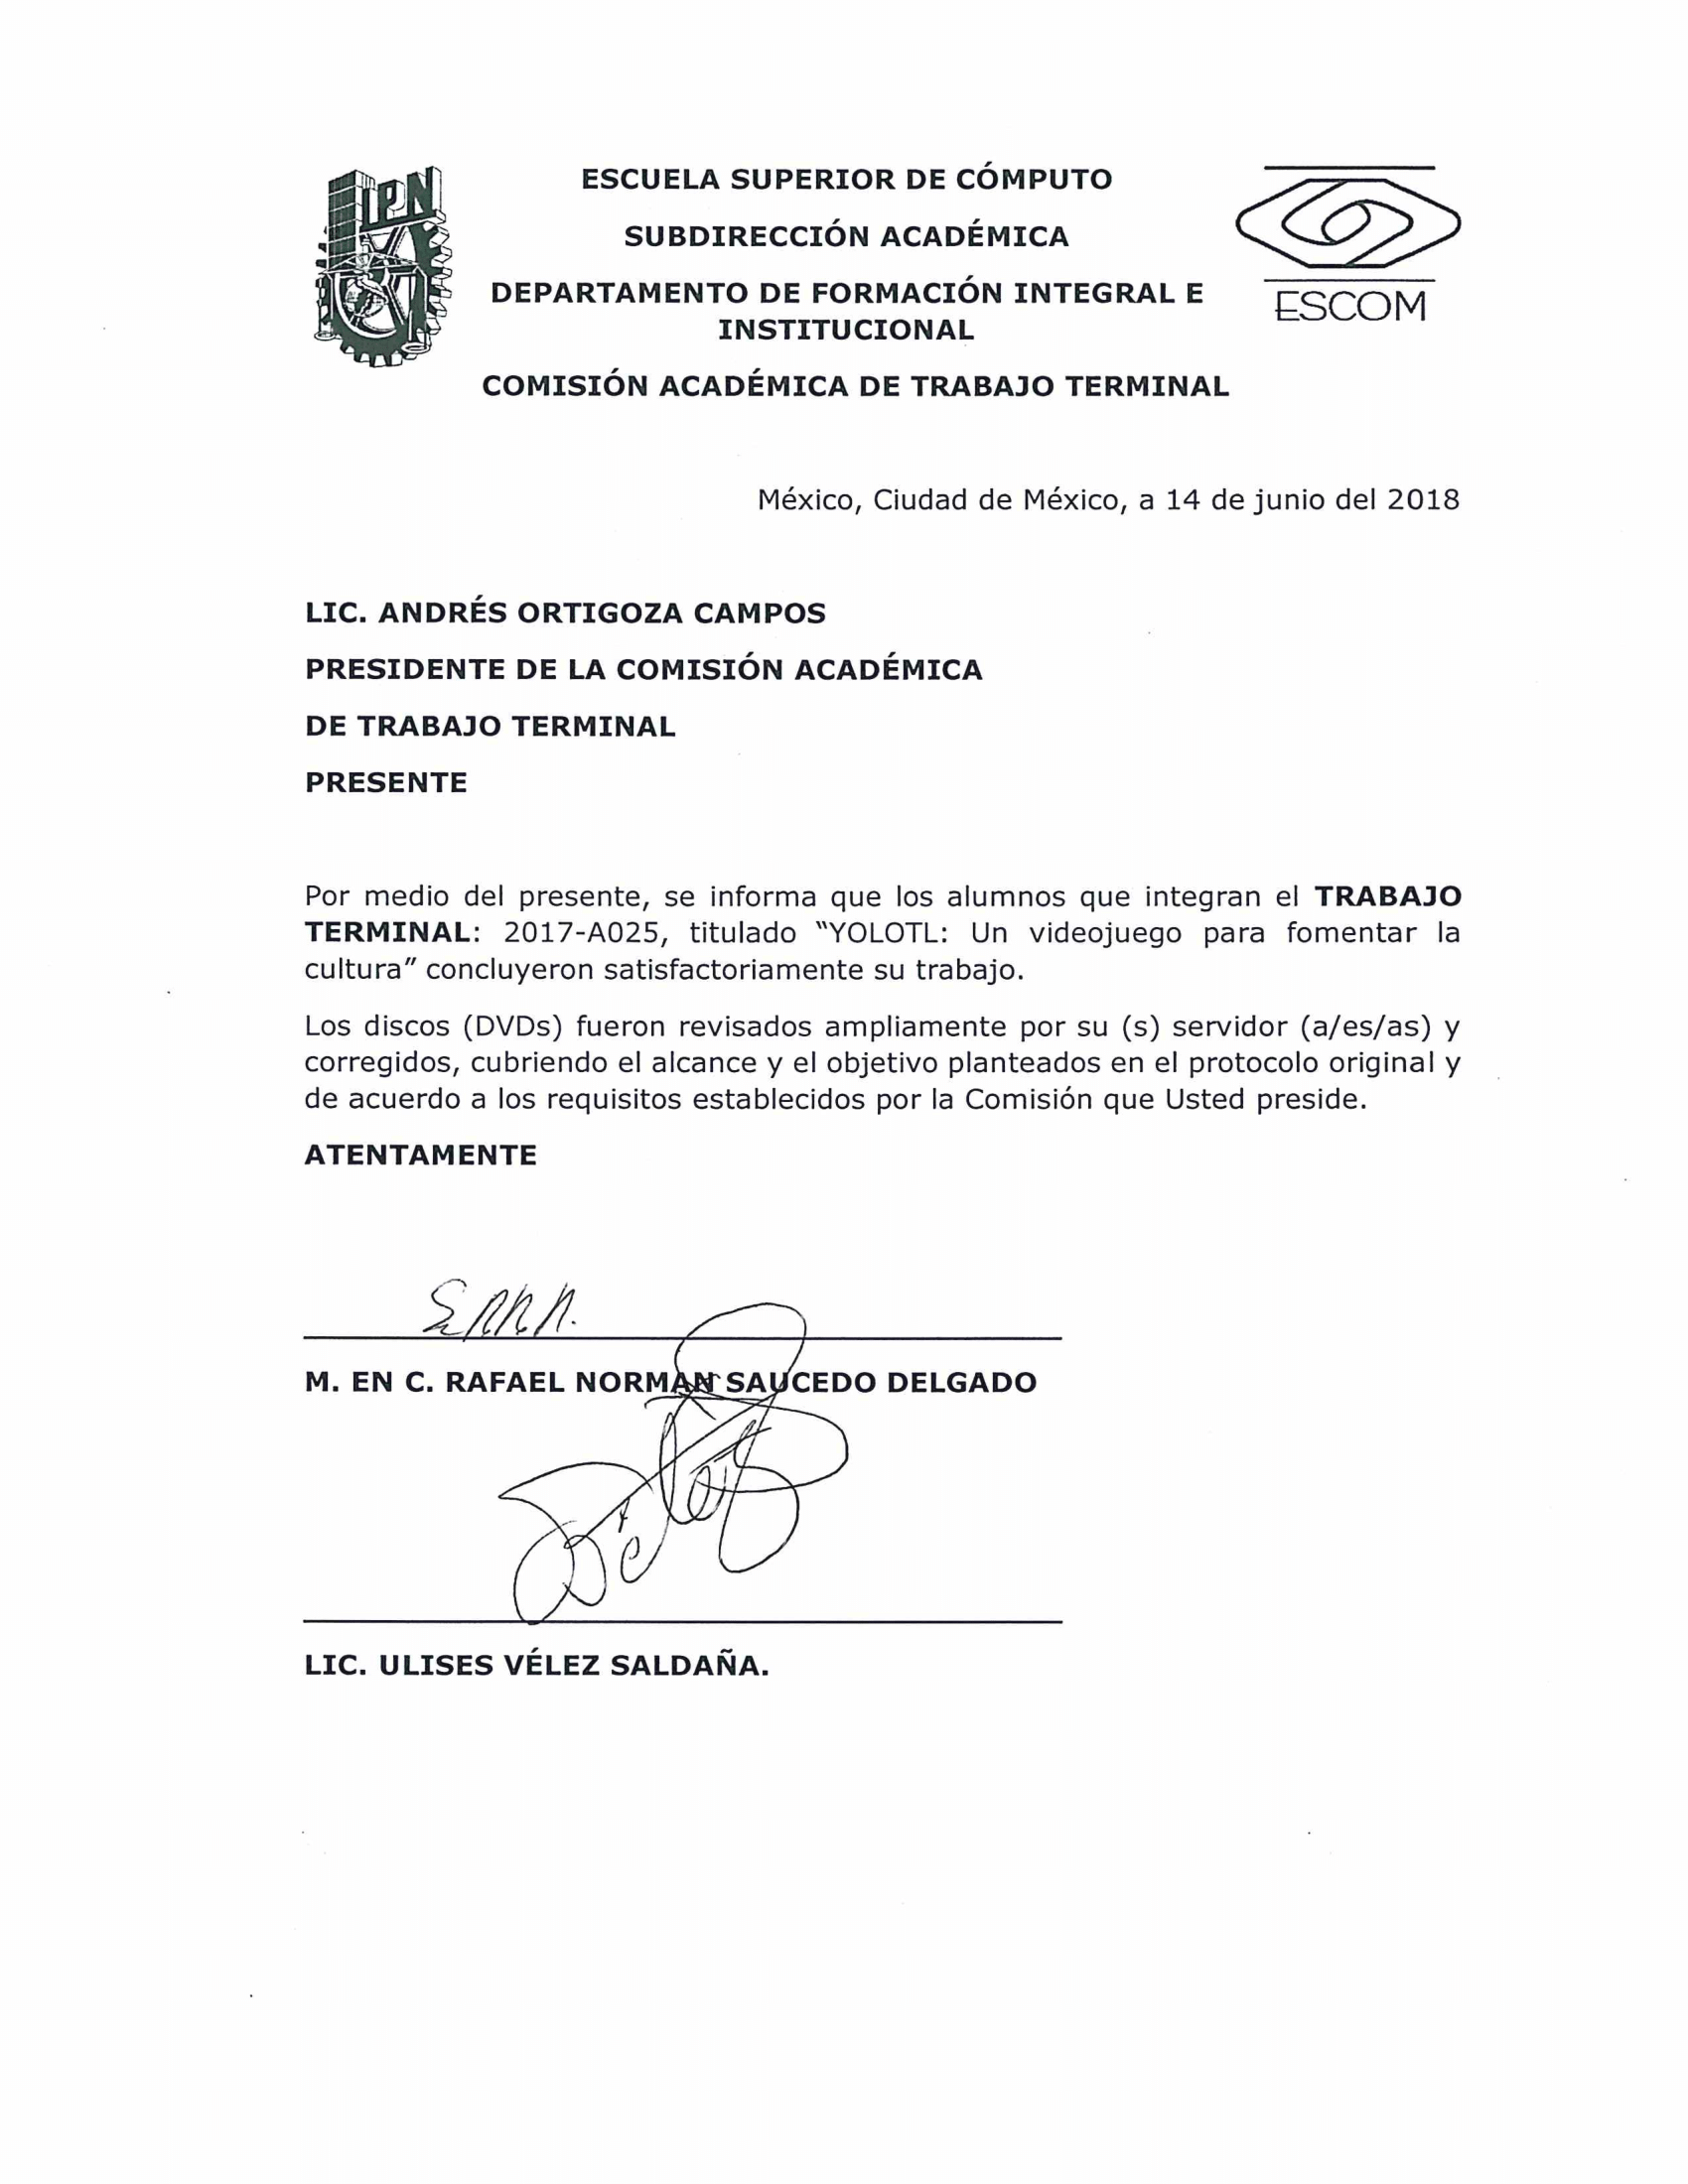
\includegraphics[width=1\textwidth]{imagen/compromiso.png}
\end{figure}

\chapter{Advertencia}

%\fcolorbox{red}{white}{
``Este documento contiene información desarrollada por la Escuela Superior de Cómputo del Instituto Politécnico Nacional, a partir de datos y documentos con derecho de propiedad y por lo tanto, su uso quedará restringido a las aplicaciones que explícitamente se convengan.”  La aplicación no convenida exime a la escuela su responsabilidad técnica y da lugar a las consecuencias legales que para tal efecto se determinen. Información adicional sobre este reporte técnico podrá obtenerse en: La Subdirección Académica de la Escuela Superior de Cómputo del Instituto Politécnico Nacional, situada en Av. Juan de Dios Bátiz s/n Teléfono: 57296000, extensión 52000.
%}

	\chapter{Introducción}
	\chapter{Planteamiento del problema} 

Hoy en día en México, la sociedad no tiene ningún interés por conocer o realizar actividades culturales. Tomaremos como actividades culturales a aquellas de aspecto artístico o histórico como obras de arte, literatura, música, danza, exposiciones y proyecciones audiovisuales. A continuación hablarémos sobre el contexto que rodea esta problemática, sus causas, consecuencias y la solución que proponemos.
\\[1pt]

\section{Contexto}
La diversidad cultural según el Movimiento Nacional por la Diversidad Cultural de México(MNDCM) es la múltiple cantidad de formas de expresión entre grupos y sociedades\cite{pp05}. La diversidad se manifiesta a través de distintos modos de creación artística, producción, difusión y distribución de dichas expresiones. La diversidad cultural es vital para el desarrollo de cualquier comunidad, pues es fuente de creatividad, innovación, originalidad, intercambio y enriquecimiento.
\\[1pt]

México es conocido por ser un país muy diverso culturalmente hablando. Cada estado posee su propia cultura regional, como la música, vestimenta tradicional, comida, entre otras cosas. Entre todos los estados del país podemos ver que existen grandes diferencias y aún así se comparte una misma identidad como país.
\\[1pt]

\section{Causas}

La ignorancia cultural del país se debe a que existe un desconocimiento de desarrollo social. Es decir que la sociedad del país tampoco tiene idea sobre su situación económica, capital humano, condiciones de salud, estado de la educación y condiciones de vida, todo esto llamado comúnmente como el bienestar social.
\\[1pt]

Existe una relación directa entre el desarrollo cultural y social. Pues ambas son debido al entorno y evolución de la sociedad que involucra. Con lo anterior deducimos que el desarrollo social favorece el desarrollo cultural.
\\[1pt]

En la última encuesta de Ipsos sobre Percepción\cite{pp04} se revela que tan errónea es la interpretación que las personas tienen sobre su desarrollo social. A partir de los datos recogidos en la encuesta y su comparación con datos reales, en temas acerca de los problemas y rasgos clave de la población de su país se elaboró la gráfica \ref{fig:ipso}. Se puede observar que México ocupa el duodécimo lugar (empatado con Corea del sur) en ignorancia total de su desarrollo como país. Entonces sí existe una ignorancia sobre desarrollo social en México.
\\[1pt]

\begin{figure}
	\centering 
	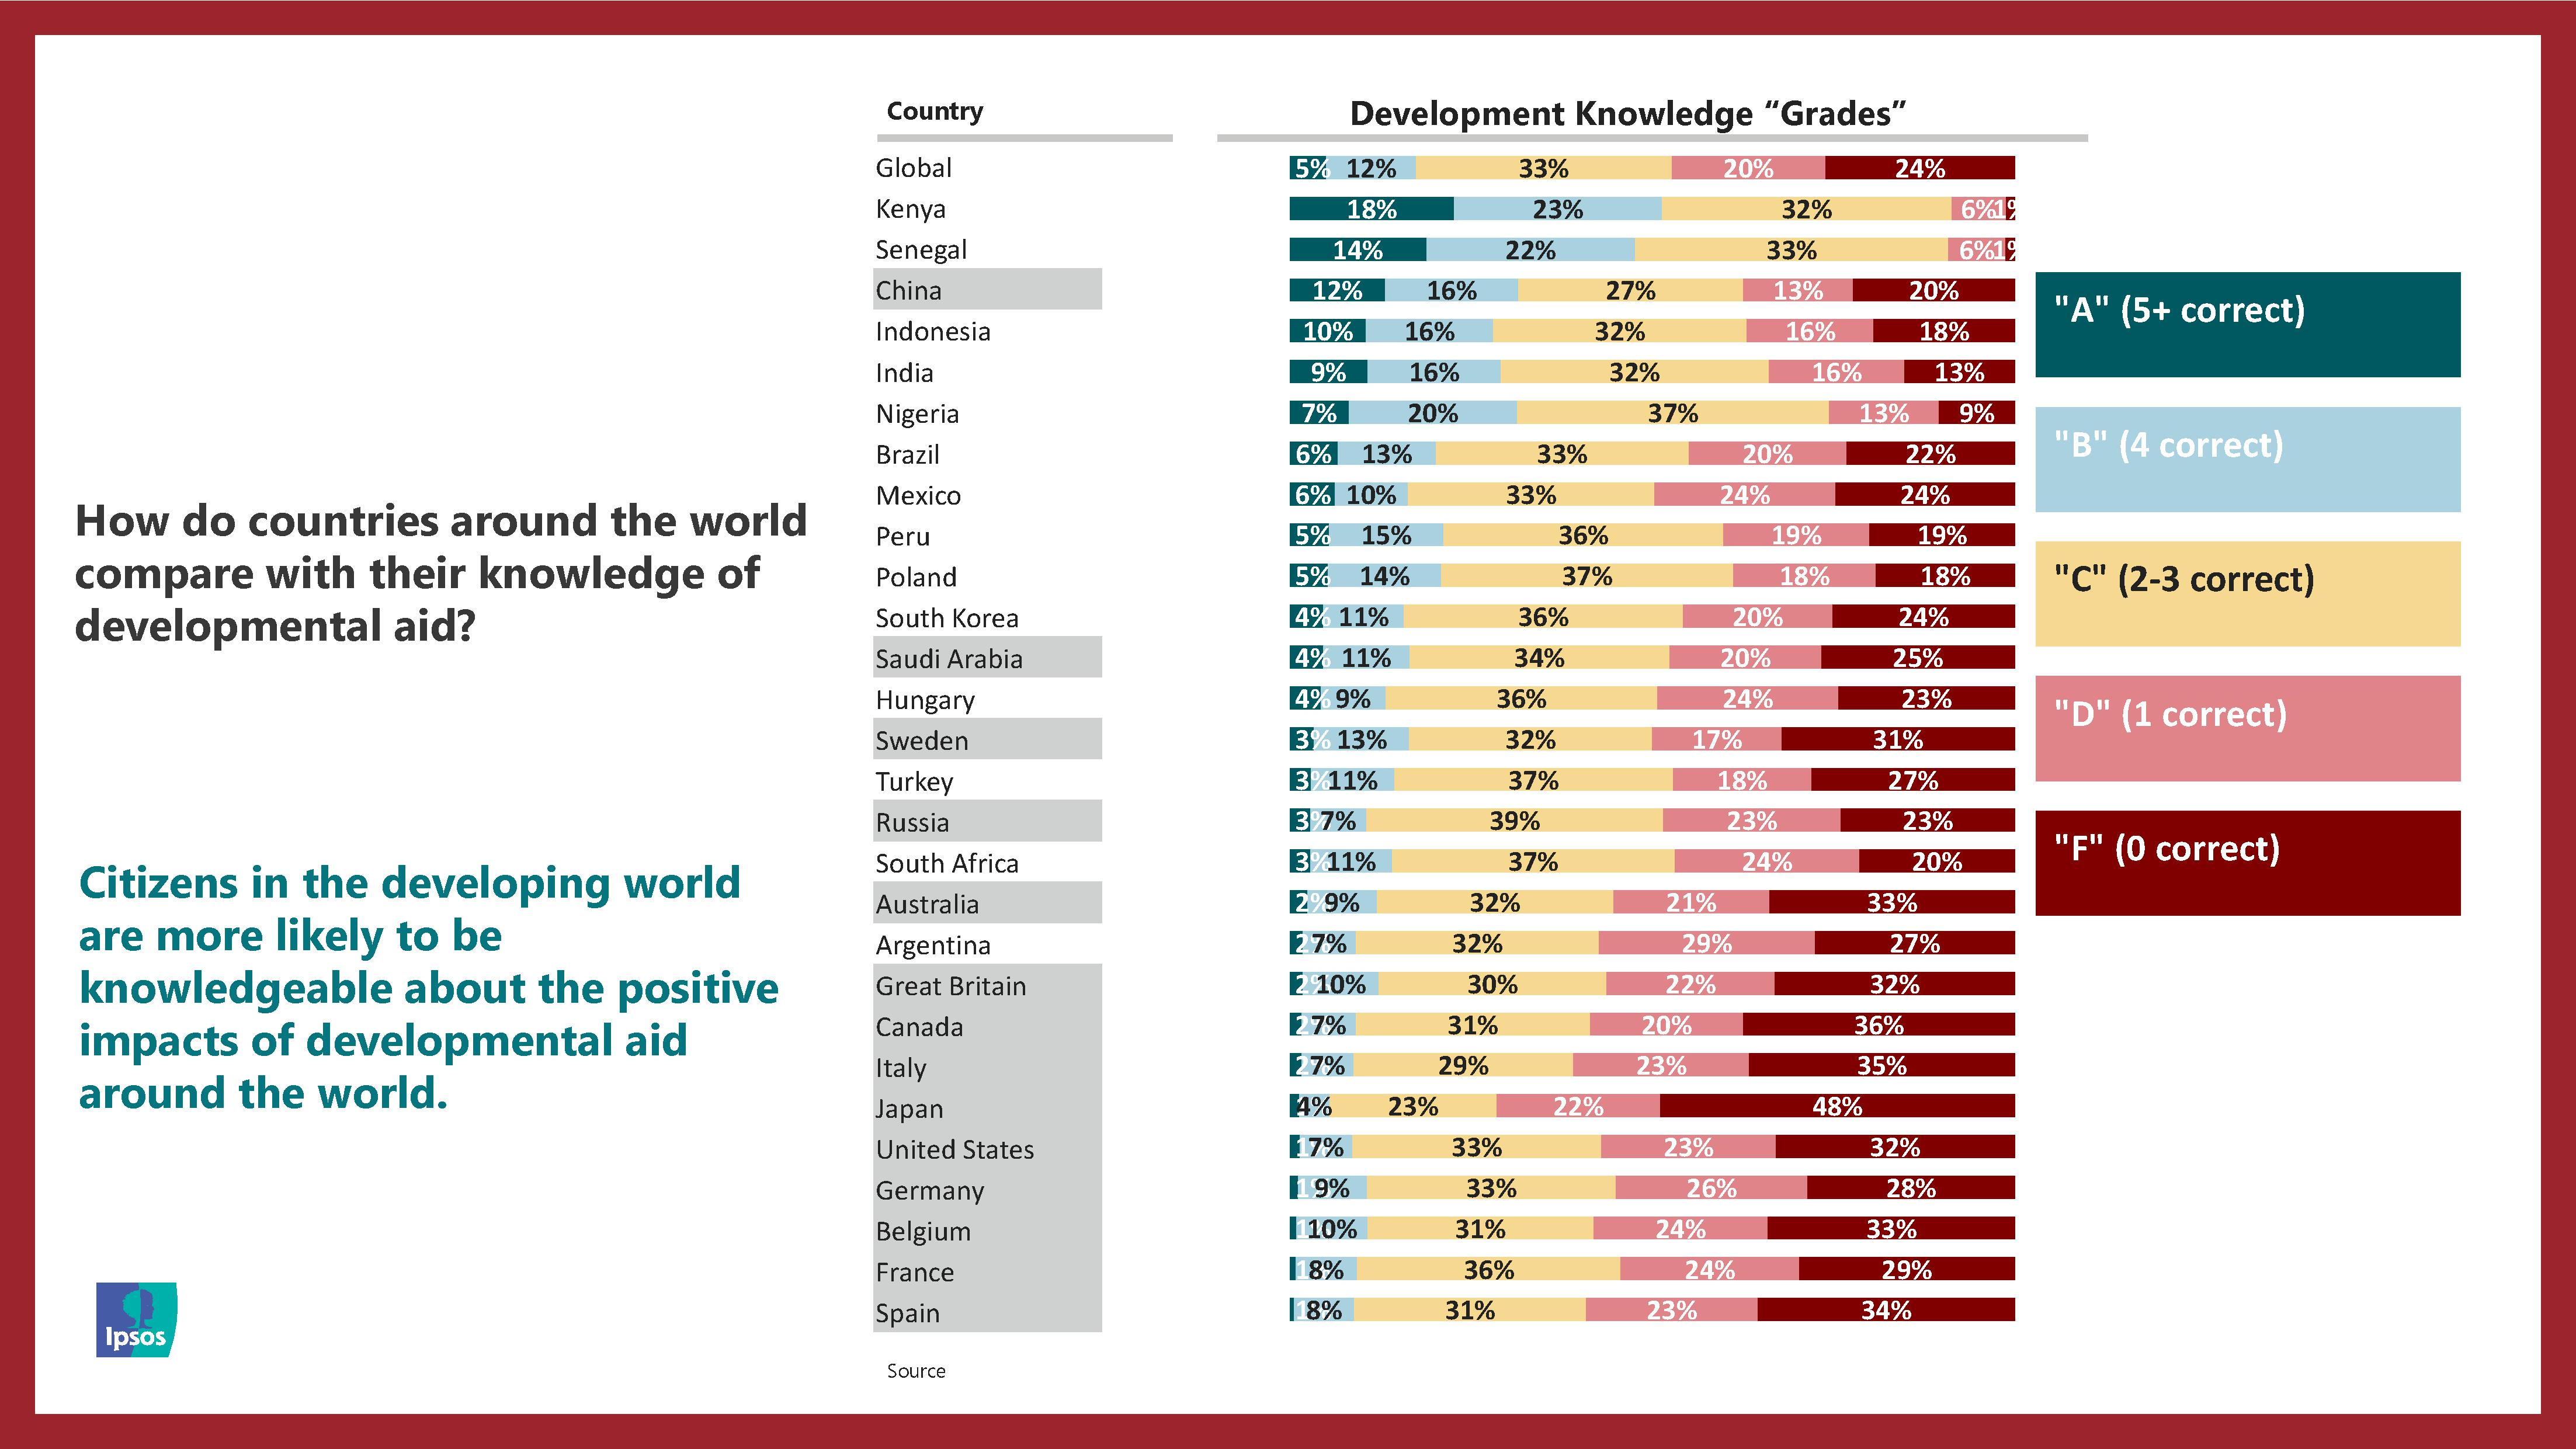
\includegraphics[width=\textwidth]{03MarcoTeorico/imageR/ipso}
	\caption{Gráfica global de la percepción de 28 paises respecto a la realidad. Donde vemos una gráfica que representa la cantidad de aciertos que tuvo la población por país en relación a la realidad.[Imagen](2017, Septiembre). Recuperado de https://www.ipsos.com/sites/default/files/ct/news/documents/2017-09/Gates\_Perils\_of\_Perception\_Report-September\_2017.pdf}
	\label{fig:ipso}
\end{figure}

\section{Consecuencias}
Ya que el desarrollo social y cultural están ligados, estos se encuentran también dependientes el uno del otro para su impulso. El movimiento cultural no solo favorecer el desarrollo recreativo si no que impulsa el desarrollo de sus naciones y viceversa. Tenemos como ejemplo en otros países del mundo, donde han sabido valorar las costumbres y tradiciones, he ahí donde nace el orgullo por su patria y se convierten en nacionalistas, demostrando el amor por su pueblo, marcando de manera definitiva el desarrollo científico, político y social de su nación\cite{pp06}.
\\[1pt]

La ignorancia cultural es el principal elemento que permite la injusticia, la enajenación y la explotación. Este fenómeno es sumamente grave y perjudicial para conformar lo que es la Identidad Cultural, la Identidad Nacional y la conciencia de la Nación. Al no saber quién es, cuáles son sus orígenes, su historia, su legado, su nombre, sus valores y principios, se le condena a la sociedad a permanentemente estar exaltando lo ajeno y despreciando lo propio.
\\[1pt]

En 2017, 41\% de los mexicanos no fue a ninguna actividad cultural según INEGI\cite{pp02}. La cifra podría leerse al revés: donde el 59\% del total de la población de 18 y más años de edad declaró que asistió a algún evento cultural seleccionado en los últimos doce meses. Pero cuando se trata de un país con una intensa vida cultural y artística, con más de 1,300 museos, alrededor de 178 zonas arqueológicas abiertas al público, 641 teatros y más de 4,000 salas de cine, de acuerdo con datos de la propia Secretaria de Cultura del gobierno federal\cite{pp01} al final queda que cuatro de cada diez personas no tienen como hábito la cultura a pesar de que varios de ellos son gratuitos.
\\[1pt]

Como ejemplo de la decadente autoconciencia cultural en México tenemos el día de la independencia. Quizá podría pensarse que todos los mexicanos saben que se festeja el 15 y 16 de septiembre. Sin embargo, los datos de la encuesta telefónica de Parametría\cite{pp03} muestran que 11\% de las personas no tiene idea de lo que se conmemora como se ve en la gráfica \ref{fig:enc01} y 57\% no sabe de que país se independizó como se ve en la gráfica \ref{fig:enc02}. Adicionalmente como podría esperarse, el nivel de escolaridad influye en el conocimiento que se tiene sobre el tema. Así, puede observarse que conforme aumenta el nivel de escolaridad se incrementa el conocimiento sobre la celebración de independencia y también sobre el país del cual se independizó México según la gráfica. \ref{fig:enc03}.
\\[1pt]

\begin{figure}
	\centering 
	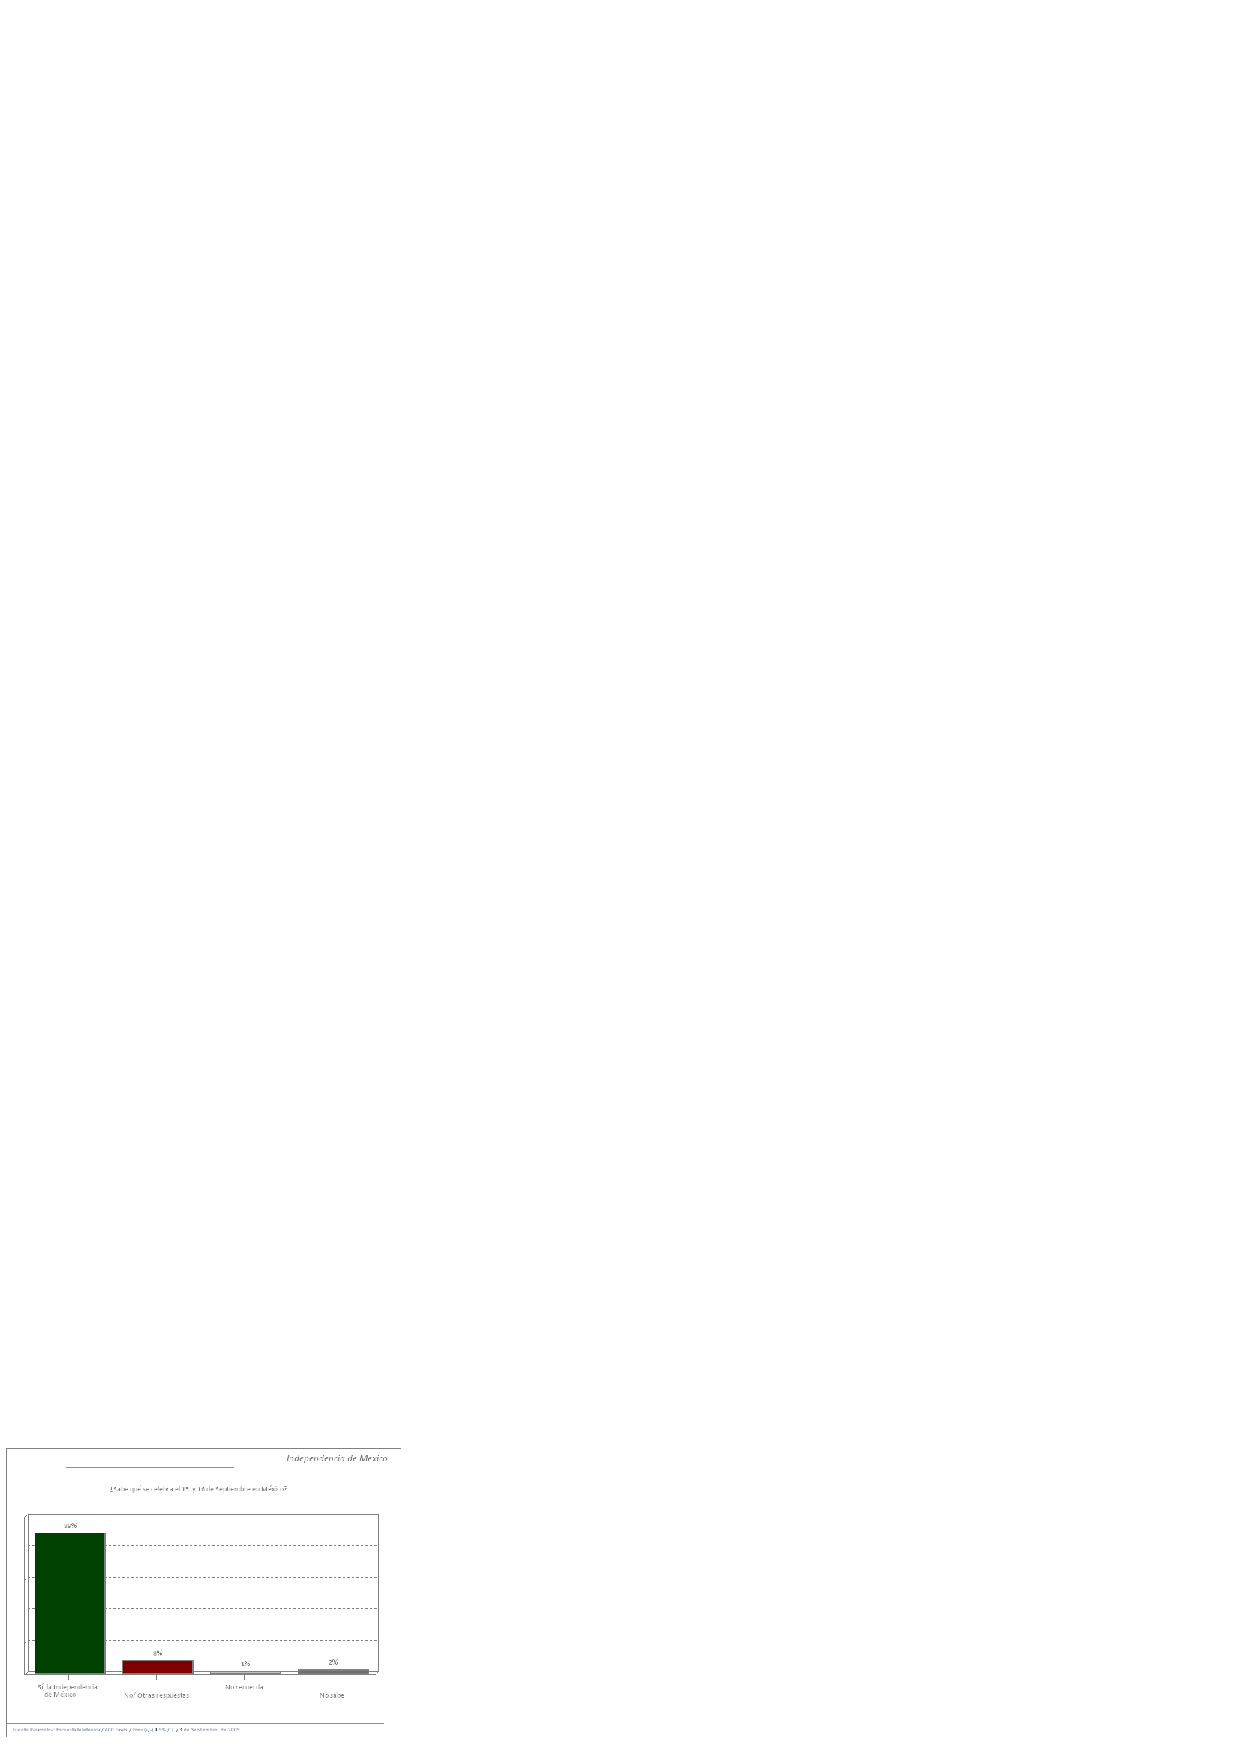
\includegraphics[width=.50\textwidth]{03MarcoTeorico/imageR/enc01}
	\caption{Gráfica a la pregunta ¿Sabe que se celebra el 15 y 16 de Septiembre en México?[Imagen](2009, Septiembre). Recuperado de: http://www.parametria.com.mx/carta\_parametrica.php?cp=4170.}
	\label{fig:enc01}
\end{figure}

\begin{figure}
	\centering 
	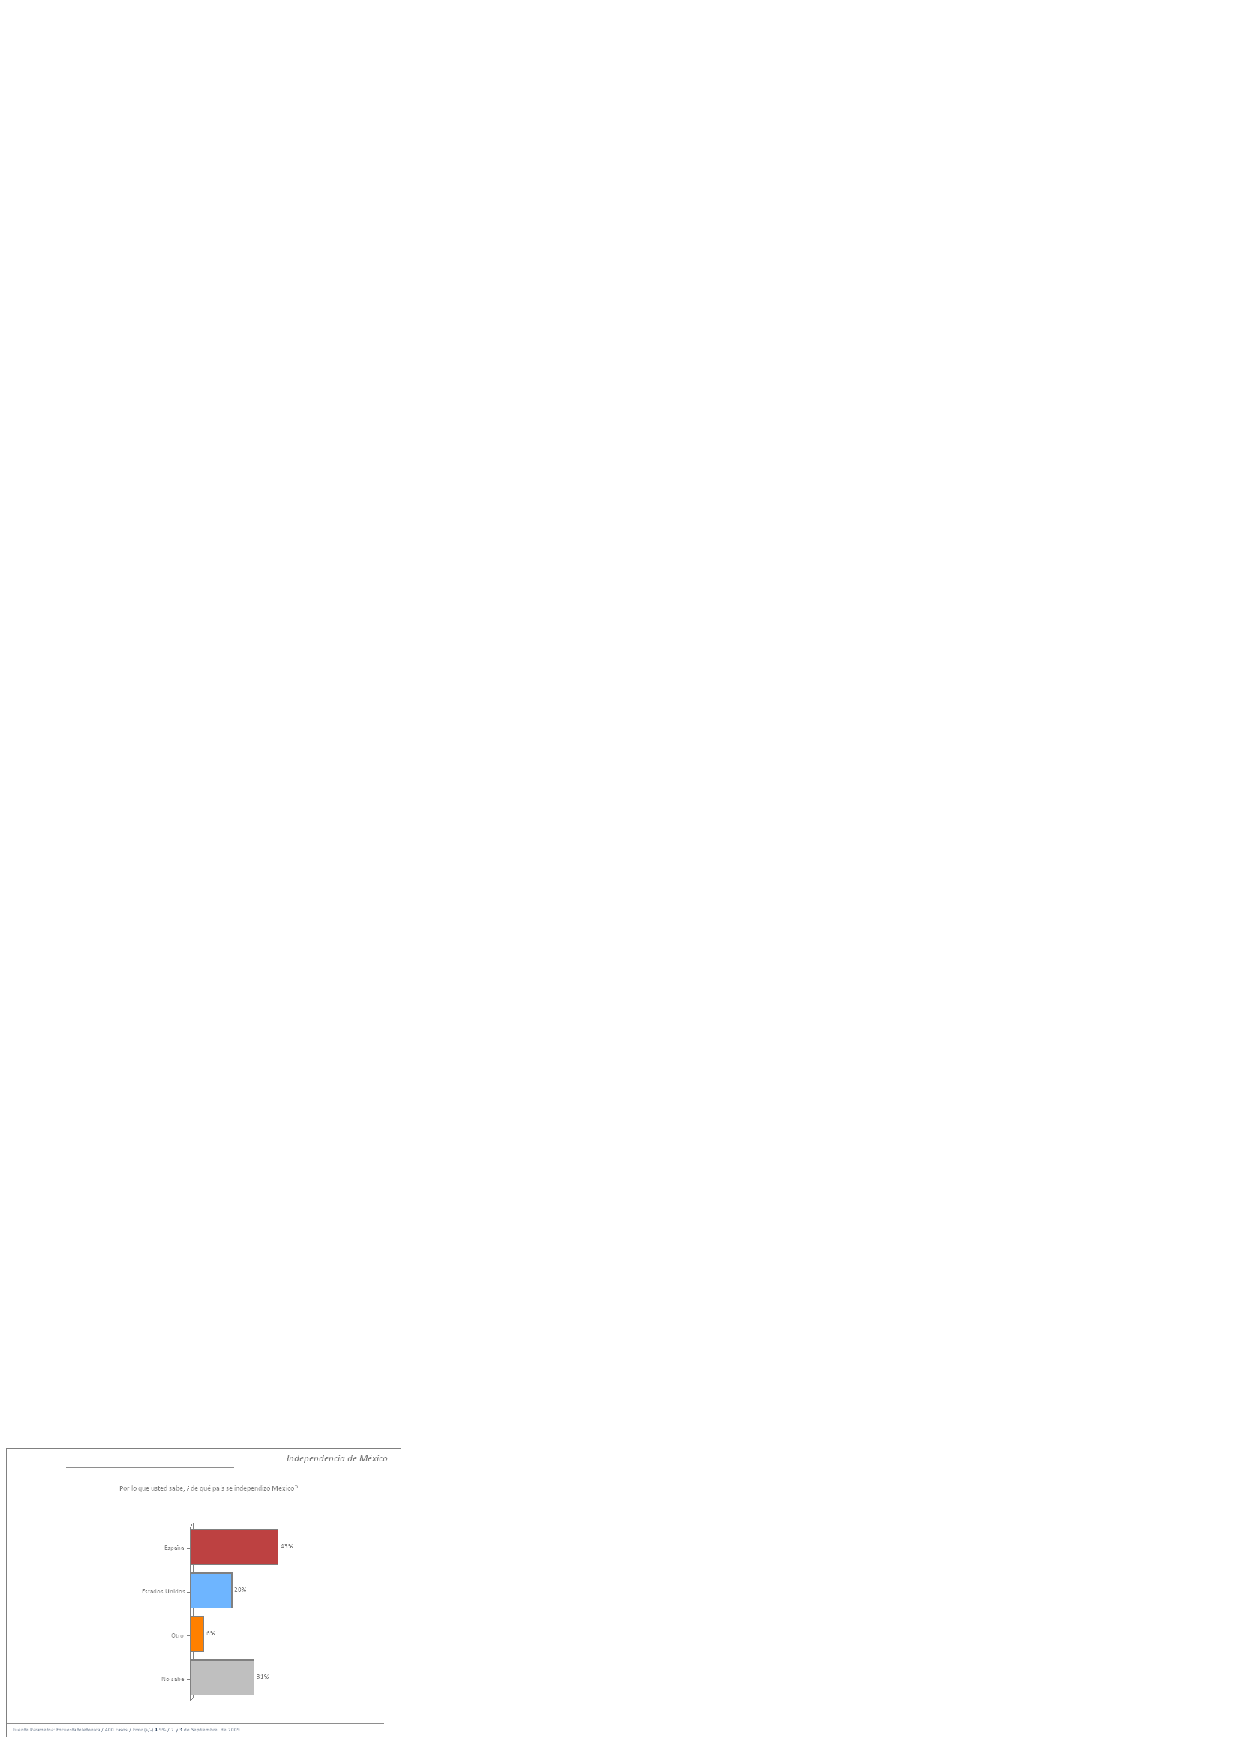
\includegraphics[width=.5\textwidth]{03MarcoTeorico/imageR/enc02}
	\caption{Gráfica a la pregunta ¿De que país se independizó México?[Imagen](2009, Septiembre). Recuperado de: http://www.parametria.com.mx/carta\_parametrica.php?cp=4170.}
	\label{fig:enc02}
\end{figure}

\begin{figure}
	\centering 
	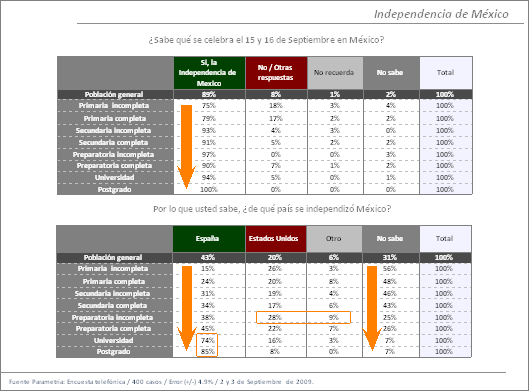
\includegraphics[width=.5\textwidth]{03MarcoTeorico/imageR/enc03}
	\caption{Gráfica de como influye la escolaridad en el conocimiento que se tiene de las fiestas patrias[Imagen](2009, Septiembre). Recuperado de: http://www.parametria.com.mx/carta\_parametrica.php?cp=4170.}
	\label{fig:enc03}
\end{figure}

Debemos saber cuál es nuestra verdadera herencia cultural y cuál nuestro legado, para preservarlo y desarrollarlo. Y como dice Guillermo Marín \cite{pp07} ``Este país se tiene que encontrar a sí mismo".
\\[1pt]


\section{Propuesta de solución}
Propondremos como solución el crear un videojuego con contexto histórico y mitológico del país prehispánico mexicano. Para esto el factor de entretenimiento y diversión lo sobrepondremos al del conocimiento o educativo.
\\[1pt]

%%%%%%%%%%%%%%%%%%%%%%%%%5YA EXISTE?
Como ejemplo similar tomaremos el videojuego llamado ``Assasins Creed II" lanzado en el año 2009, que debutó en el puesto número 1 en Estados Unidos, Canadá, Suecia, Francia, España y Australia, y dentro del «Top 50» en más de diez países. Este juego tiene como género acción-aventura, también se situa en la época renacentista y este hecho lográ que el jugador adquiera conocimientos sobre ese tiempo, tanto lugares, como personas, situación social, etc.
\\[1pt]

%%%%%%%%%%%%%%%%%%%%%%%%%%55QUE IMPLICA?
Para llevar a cabo el diseño de un videojuego los programadores son los responsables de hacer posible la interactividad entre el jugador y el sistema. Se realizará detro del proyecto la programación estructurada, orientada a objetos, modelado, arte digital, conocimiento de dispositivos móviles y animación digital. Considerando importante usar modelos matemáticos para las diferentes experiencias de juego. 
\\[1pt]

%%%%%%%%%%%%%%%%%%%%%%%%%%%%%%%VENTAJAS?
El resultado de adquisición de conocimiento en lo videojuegos se debe al cómo. En la imagen \ref{fig:conoAprendizaje} se muestra el cono de la experiencia de Edgar Dale (pedagogo) donde resaltamos que el mayor aprendizaje es por medio de la simulación.

\begin{figure}
	\centering 
	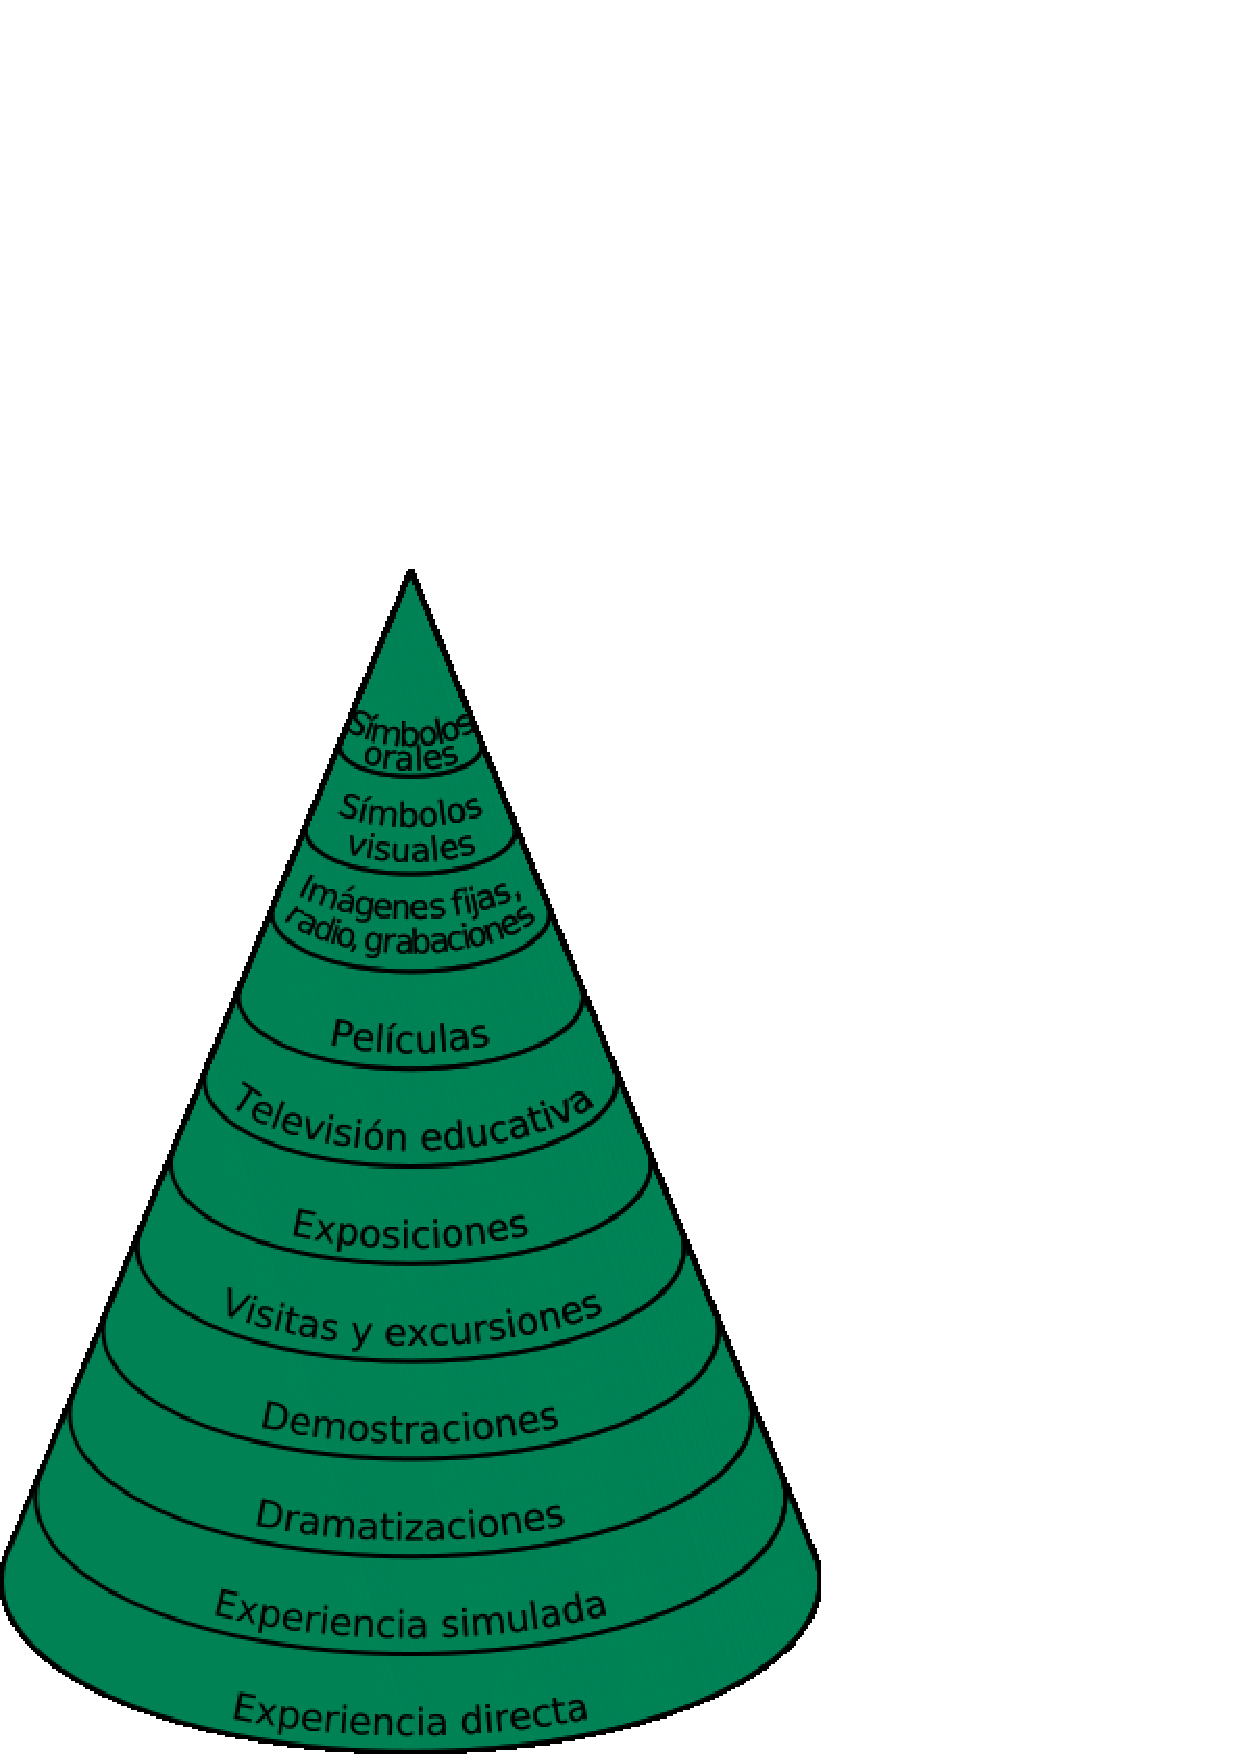
\includegraphics[width=.5\textwidth]{03MarcoTeorico/imageR/conoAprendizaje}
	\caption{Cono de la experiencia de Edgar Dale. Se muestra diferentes maneras de aprendizaje que se ordenan según su impacto de aprendizaje.[Imagen](2008). Recuperado de: https://es.wikipedia.org/wiki/Edgar\_Dale\#/media/File:Cono\_de\_la\_Experiencia.svg}
	\label{fig:conoAprendizaje}
\end{figure}

Los medios audiovisuales son los que mayor impacto tiene en difusión cultural como se ve en la gráfica de la imagen \ref{fig:modecult}. Así podemos ver una potencial herramienta para insitar a la participación en los eventos culturales, pues los videojuegos son medios audiovisuales.
\\[1pt]

\begin{figure}
	\centering 
	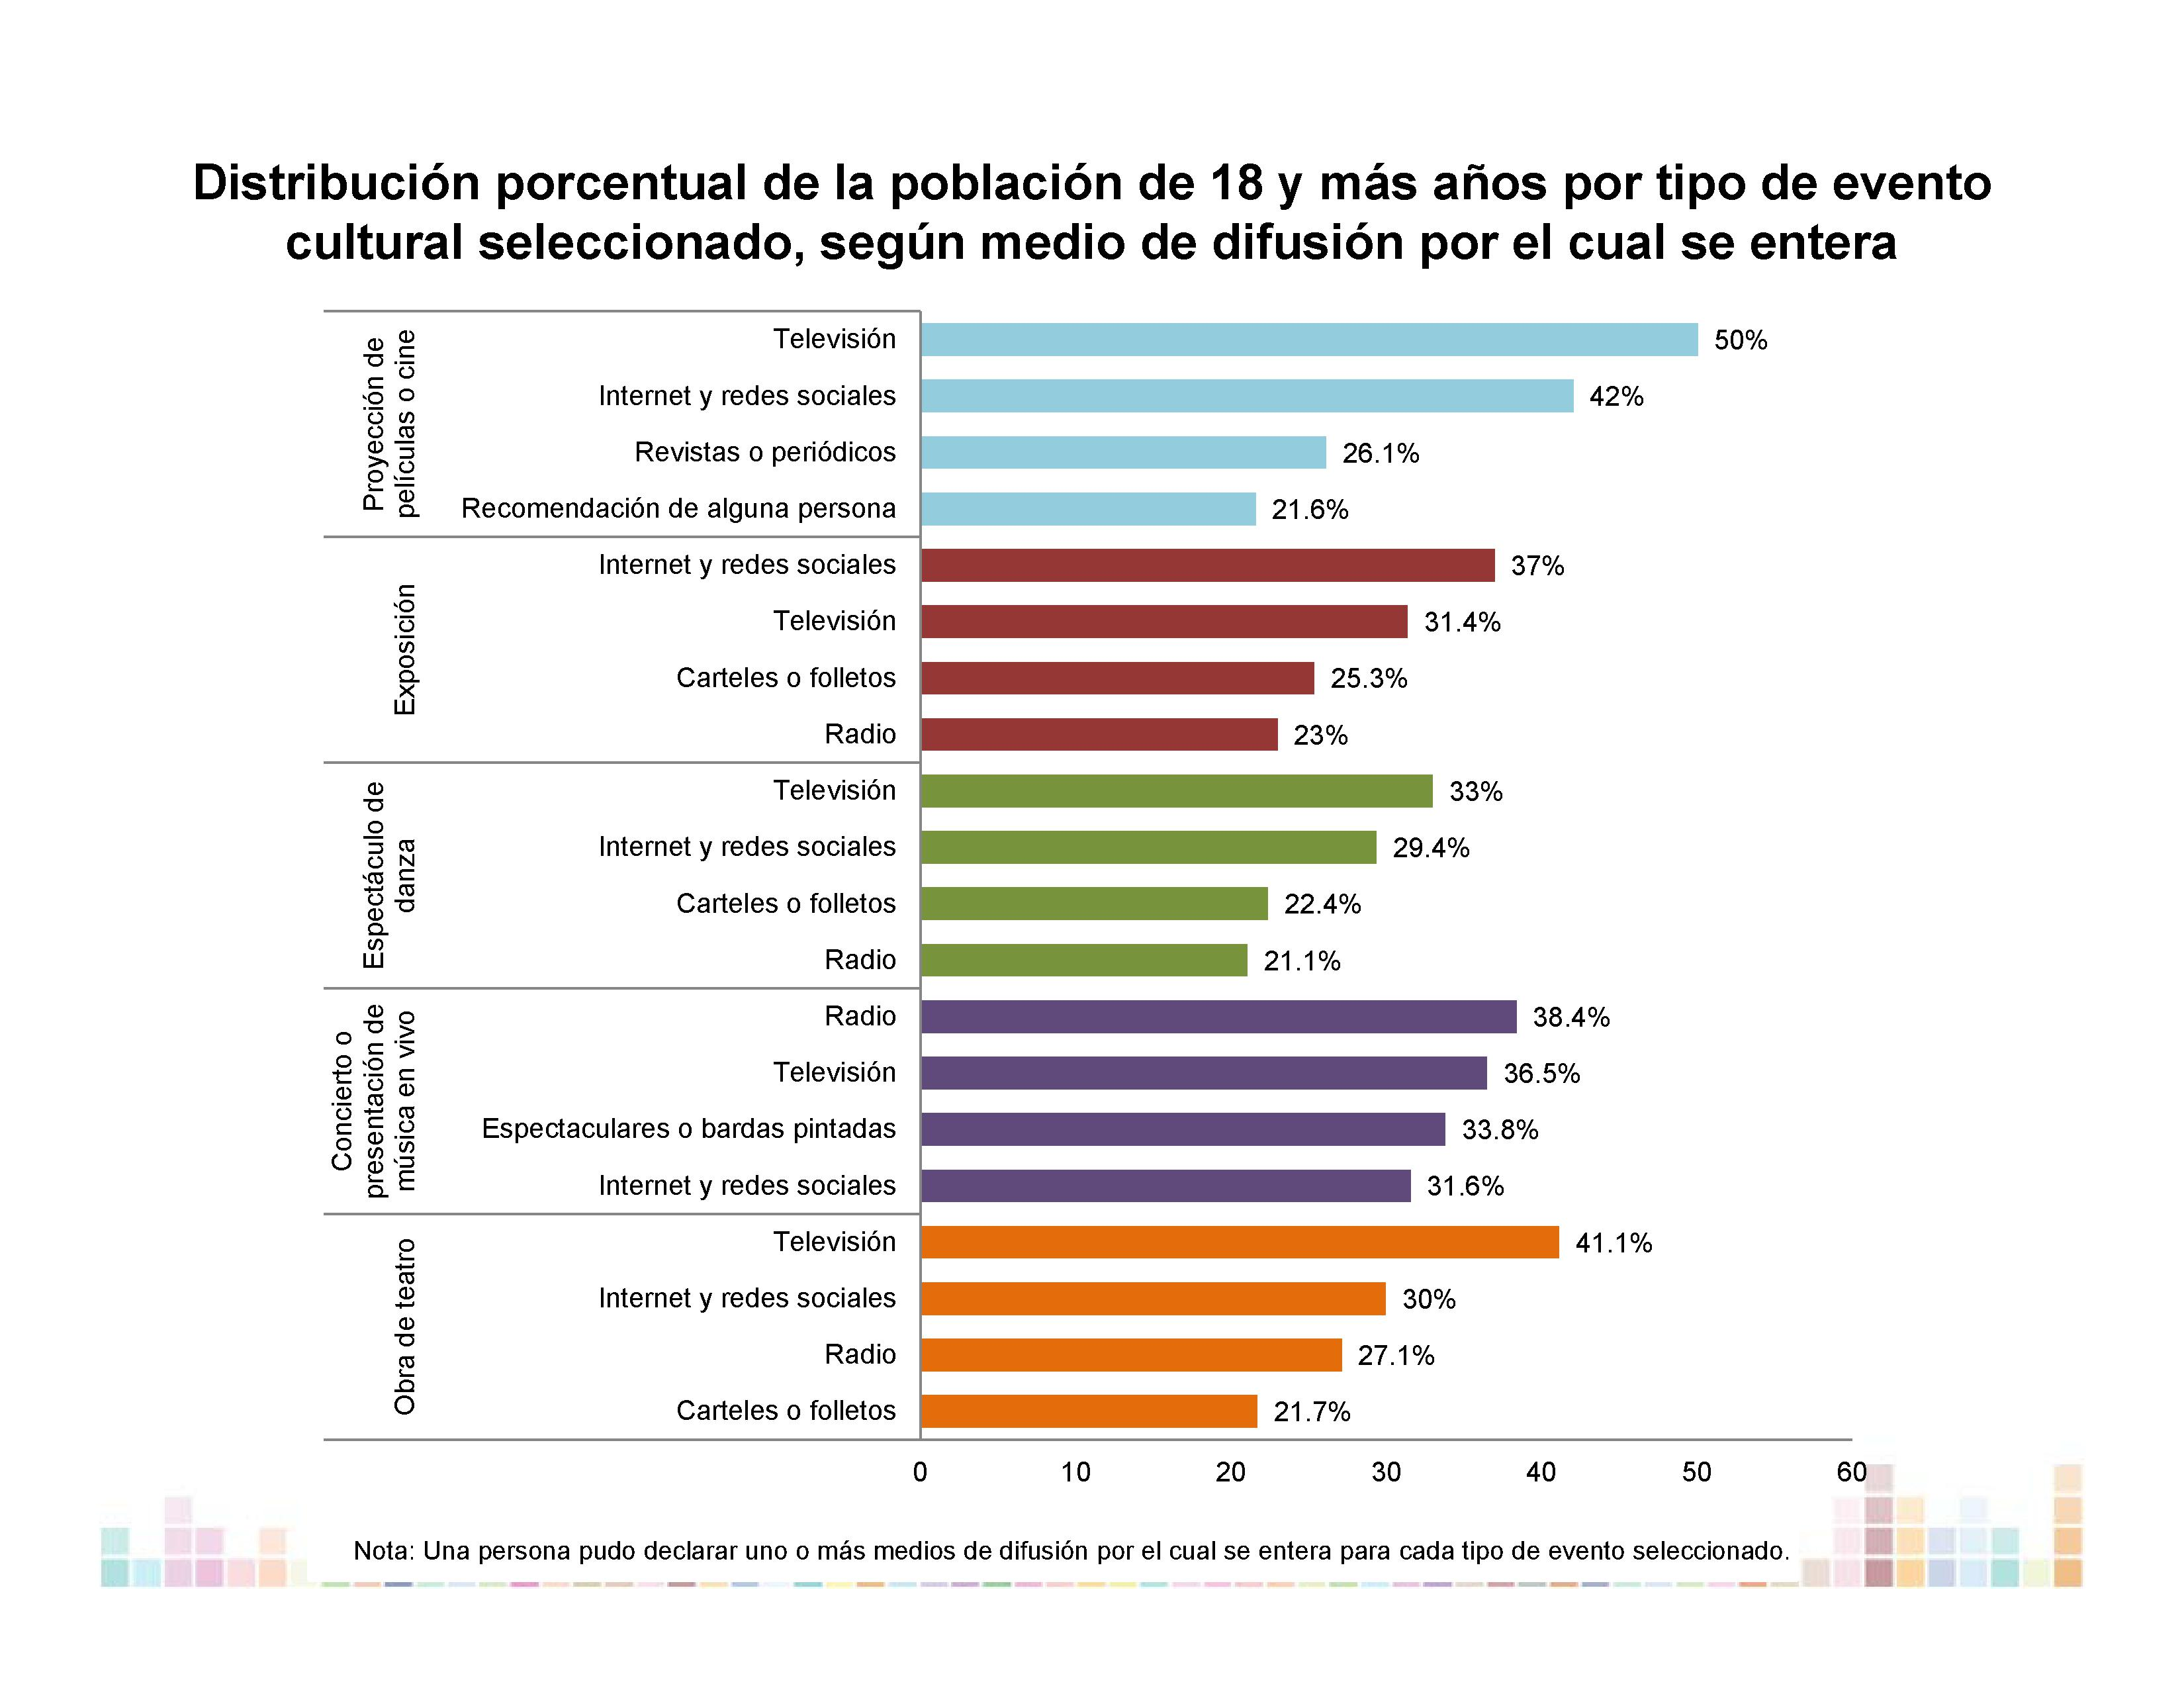
\includegraphics[width=.75\textwidth]{03MarcoTeorico/imageR/modecult}
	\caption{Encuesta MODECULT en asistencia por tipo de evento y medio de difusión por el cual se ha enterado.[Imegen](2017, Mayo). Recuperado de: http://internet.contenidos.inegi.org.mx/contenidos/productos/prod\_serv/contenidos/espanol/bvinegi/productos/nueva\_estruc/promo/resultados\_modecult\_may2017.pdf}
	\label{fig:modecult}
\end{figure}

También otra de las ventajas es la cantidad de gente que juega videojuegos en México y el dispositivo por el cuál lo consumen como lo muestra la imagen \ref{fig:consumo30}. Donde el 20\% de los mexianos consumen videojuegos y 45\% de ellos se juegan en dispositivos móviles.

\begin{figure}
	\centering 
	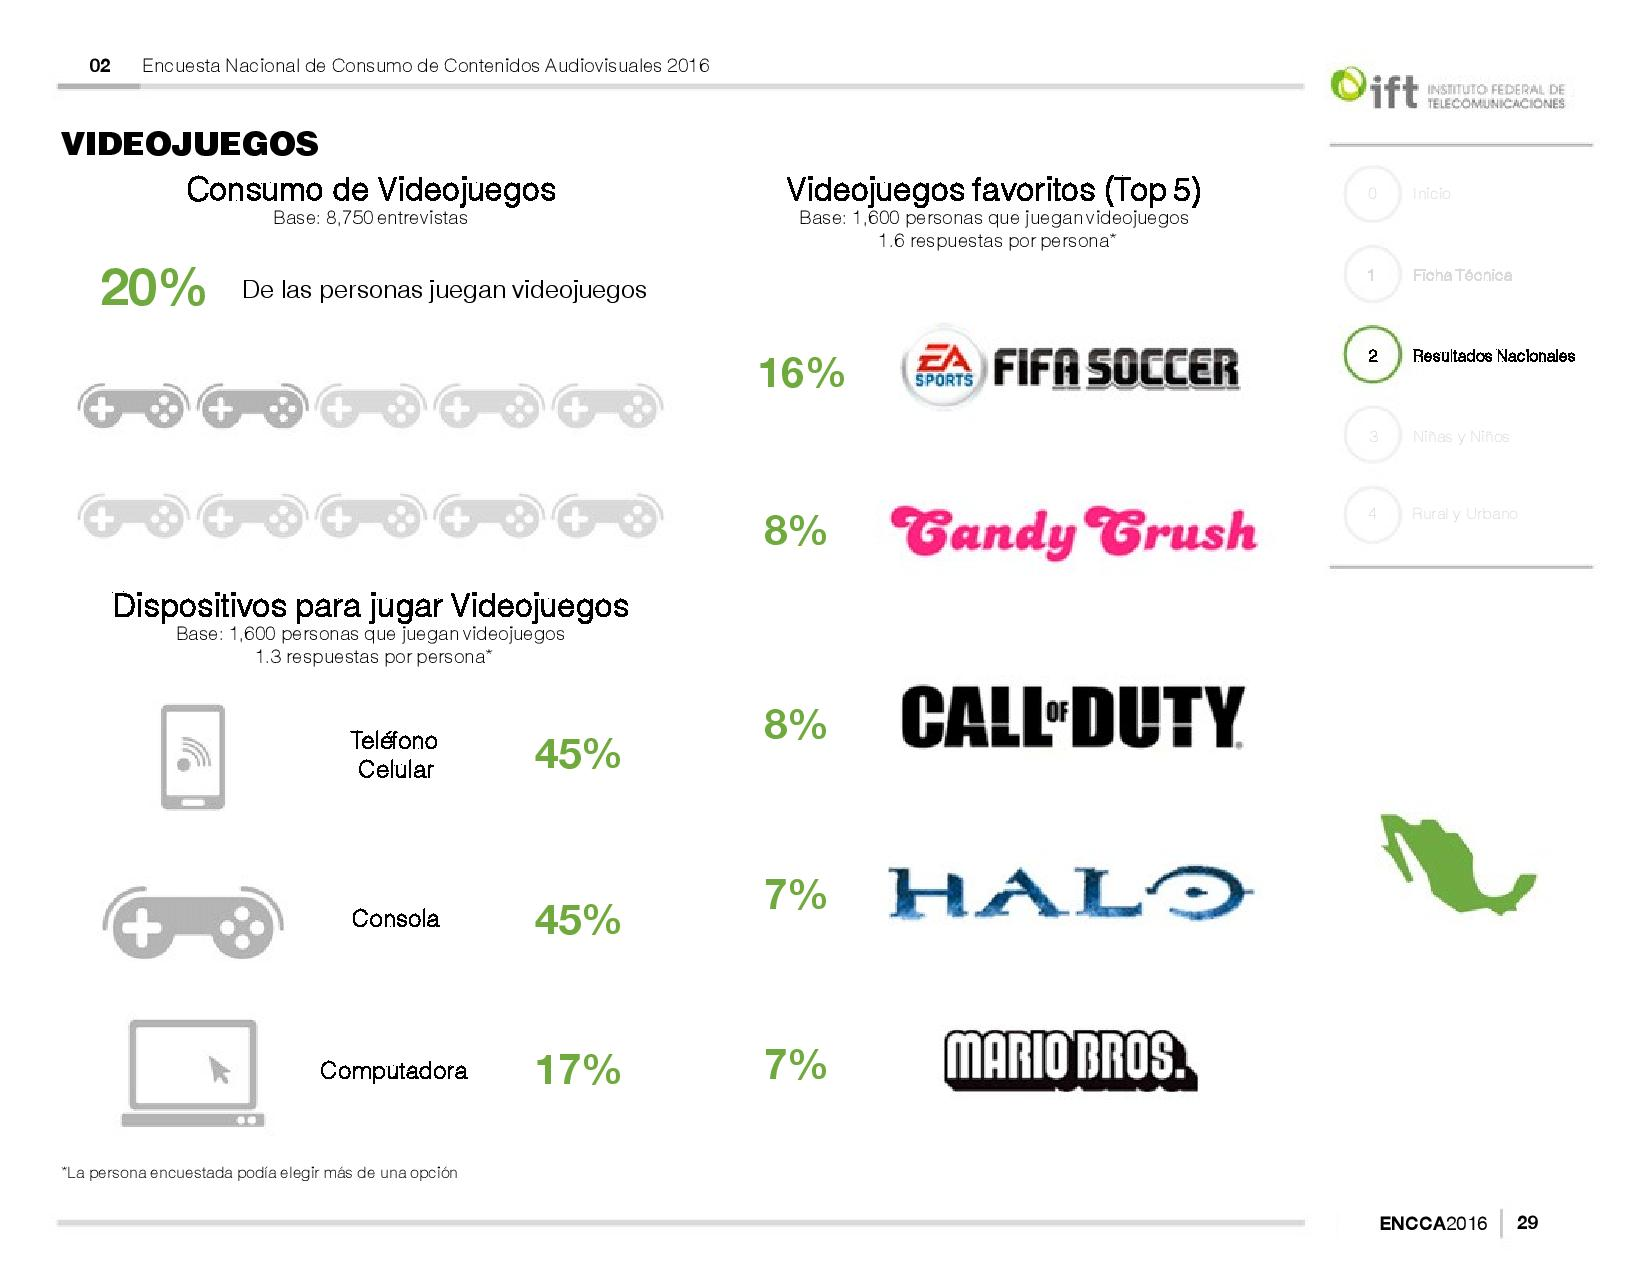
\includegraphics[width=.75\textwidth]{03MarcoTeorico/imageR/consumo30}
	\caption{Encuesta Nacional de Consumo de Contenidos Audiovisuales, donde muestra el consumo de videojuegos[Imegen](2016). Recuperado de: http://www.ift.org.mx/sites/default/files/encca2016\_vf-compressed.pdf}
	\label{fig:consumo30}
\end{figure}

%%%%%%%%%%%%%%%%%%%%%%%%%%DESVENTAJAS?

Una desventaja de los videojuegos en cuestión de desarrollo es que son un complejo sistema tecnológico que combina diversos elementos: visuales, matemáticos, físicos, electrónicos o narrativos, entre otros muchos para generar una experiencia controlada porel jugador para su mayor entretenimiento. Por tanto existe una complejidad al unir de forma adecuada todos esos elemntos para crear una gran experiencia de diversión para los jugadores, se necesita de una gran cantidad de talentos diversos o multidisciplinarios, los cuales no se abarcarán todos ellos.

También se debe tomar en cuenta que existe una gran cantidad de gustos e intereses entre los jugadores existentes y no se puede aplicar todos los existentes.

La mejora de las condiciones de un producto en un videojuego resulta esencial. Por esta misma razón el tiempo de desarrollo siempre es muy largo y en la mayoría de las ocasiones tiene muchos contratiempos que provocan retrasos de lanzamiento o incluso rediseños completos.




	\chapter{Marco teórico conceptual}
	\section{Videojuegos}
\subsection{Definición}
\subsection{Clasificación}
\subsection{Industria en México}

	\section{Desarrollo de videojuegos}
	En sus inicios los videojuegos se encontraban fuertemente ligados al hardware y no eran los complejos sistemas actuales; por lo tanto, la naciente industria de los videojuegos no tenía la necesidad de documentar sus productos como sistemas de software. Es a partir de la segunda mitad de la década de los 80’s con la llegada de Nintendo que el videojuego da sus primeros pasos como sistema complejo de software [ ]. Si bien Nintendo inicio el videojuego como medio argumental y de entretenimiento, no fue esta compañía la que iniciaría la producción sistematizada del videojuego, tal merito se lo lleva la compañía ID Software con el lanzamiento de Doom en la década de los 90’s, siendo el primer videojuego diseñado bajo una arquitectura orientada a la reutilización. Dicha arquitectura consistía en separar el software en una serie de módulos con funcionalidad especifica de tal suerte que dichos módulos se pudieran reutilizar en proyectos de temática parecida sin que se tuviera que modificar directamente el código, limitando al equipo de programadores únicamente a agregar módulos nuevos que complementaran la funcionalidad [ ]. Naciendo así la necesidad de documentar los videojuegos como sistemas de software. La década de los 90’s es un segundo punto de inflexión en la industria, pues hasta ese momento el mercado había sido dominado por compañías como Nintendo y SEGA. En 1994 PlayStation de la compañía SONY llega al mercado de los videojuegos y con esta consola se abre la puerta a títulos de carácter más maduro, iniciando así la masificación de los videojuegos [ ]. Con la llegada de las computadoras personales, el XBOX de Microsoft y el boom del internet la industria del videojuego volvió a adaptarse al mercado. 
\\
\par
Del anterior párrafo puede concluirse que la industria de los videojuegos tuvo que pasar por diferentes cambios para comenzar a implementar metodologías de desarrollo de videojuegos y herramientas que le permitieran a las compañías optimizar recursos y tiempos[ ]. 
\subsection{Metodologías de desarrollo}

\input{03MarcoTeorico/03DesarrolloVideojuego/Metodologias/01Cascada}
\input{03MarcoTeorico/03DesarrolloVideojuego/Metodologias/02Scrum}
\input{03MarcoTeorico/03DesarrolloVideojuego/Metodologias/03XP}
\input{03MarcoTeorico/03DesarrolloVideojuego/Metodologias/04Huddle}



	\subsection{Pipeline}
	\subsection{Motores gráficos}
	\input{03MarcoTeorico/03DesarrolloVideojuego/MotoresGraf/01motorGrafico}
	\input{03MarcoTeorico/03DesarrolloVideojuego/MotoresGraf/02ArqutecturaMotor}
	\input{03MarcoTeorico/03DesarrolloVideojuego/MotoresGraf/03Motores}
	\subsection{Software auxiliar}
	\section{Gamificación}
La gamificación es el uso de las mecánicas de juego en entornos ajenos al juego, según el término anglosajon definido por Sebastian Deterding (Diseñador/investigador del diseño de juego para el florecimiento humano) \cite{gameDef}. Es decir, que cualquier tema o asunto a tratar puede pasar por un proceso para convertirse en un juego. Y deben de cumplir con características específicas según el profesor Santiago Moll\cite{gameficacion}, estas son: mecánicas o reglas, dinámicas de juego, y componentes. También describe que clase de jugadores existen, el proceso que debe de llevar un tema a gamificar y la finalidad que debe cumplir. Todo esto se muestra a continuación.
\\[1pt]

\subsection{Característcas}
Las características a presentar son una guía para realizar un juego y no necesariamente se debe cumplir con todas y cada una de ellas. Sin embargo estas características ayudan en gran medida al entretenimiento del jugador. Recordemos que las características a presentar incluyen las mecánicas o reglas, dinámicas de juego y componentes.
\\[1pt]
 
\textbf{Mecánicas o reglas}
\\[1pt]
Son las normas de funcionamiento que permiten se adquiera un compromiso del jugador con el juego. Mantienen al jugador en constante actividad y le permite ver los límites que existen en el juego.
\\[1pt]

\begin{itemize}
	\item Colección: Logros y recompensas que consigue el jugador.
	\item Puntos: Para motivación y conteo de realizar una tarea por el jugador.
	\item Ranking: Clasificación o comparación entre jugadores.
	\item Nivel: Reflejan el progreso del jugador.
	\item Progresión: Consiste en completar el 100\% de la actividad encomendada al jugador.	
\end{itemize}

\textbf{Dinámicas de juego}
\\[1pt]
Motivan y despiertan el interés del jugador de realizar una actividad dentro del juego. Aunque no es necesario cumplir con este requisito para un juego son clave para mantener jugando a la persona.  

\begin{itemize}
	\item Recompensa: Premio por realizar alguna actividad en el juego.
	\item Competición: Deseo de estar en una determinada posición o grado en el juego entre los participantes.
	\item Cooperativismo: Otra forma de competir pero en un grupo de jugadores con un mismo fin o meta del juego.
	\item Solidaridad: Se fomenta la ayuda entre jugadores y debe ser de manera altruista.
\end{itemize}

\textbf{Componentes}
\\[1pt]
Los componentes se encargan de personalmente darle a cada jugador su estado en el juego. Así son identificados por los demás participantes fácilmente en las actividades que destacan o han realizado con exito. También cumplen con la parteen la que el jugador puede proyectarse dentro juego.
\begin{itemize}
	\item Logros: Visualizan el alcance del jugador de un objetivo del juego.
	\item Avatares: Representación gráfica del jugador.
	\item Medallas: Insignia o distintivo del jugador que ha ganado.
	\item Desbloqueo: Permiten avanzar en las actividades del juego gracias a actividades previas hechas por el jugador.
	\item Regalos: Un presente por la realización correcta de un reto por el jugador	.
\end{itemize}

\subsection{Tipos de jugadores}
Para saber que elementos debe llevar el juego a realizar debe conocerse los tipos de jugadores que existen. También se debe de saberse las motivaciones que los impulsan a seguir jugando. A continuación se muestran cuatro identificados.
\begin{itemize}
	\item Triunfador: Su finalidad es la consecución de logros y retos.
	\item Social: Le encanta interactuar y socializarse con el resto de compañeros.
	\item Explorador: Tiene tendencia a descubrir aquello desconocido.
	\item Competidor: Su finalidad es demostrar su superioridad frente a los demás.
\end{itemize}


\subsection{Proceso}
Ahora se seguirá los pasos para convertir un tema a un juego. Conociendo ya los elementos que disponemos y haber identificado al tipo de jugador que queremos, podemos convertir nuestro tema o actividad en un juego. 
\begin{itemize}
	\item Viabilidad: Determinar si el contenido que se quiere enseñar es jugable.
	\item Objetivos: Definir los objetivos del juego.
	\item Motivación: Valorar la predisposición y el perfil de jugadores.
	\item Implementación: Relación entre el juego y contenido a enseñar.
	\item Resultados: Evaluación de la actividad en el juego.
\end{itemize}


\subsection{Finalidad}
En cada juego se debe tener claro lo que quiere lograrse, es decir la finalidad del juego. Debe de determinarse que se desea lograr con el jugador.
\begin{itemize}
	\item Fidelización: Establecer un vínculo del contenido del juego con el jugador.
	\item Motivación: Crear una herramienta contra el aburrimiento del contenido a tratar.
	\item Optimización: Recompensar al jugador en aquellas tareas en las que no tiene previsto ningún incentivo.
\end{itemize}

	\section{Cultura}

	\section{Cultura Digital}
La misión de la cultura digital es generar a través del espacio físico y de plataformas virtuales, programas enfocados al uso creativo y crítico de la tecnologías digitales como herramientas de producción y transformación cultural \cite{vid08}. El objetivo ha ido precisamente cubrir el déficit de investigación que hay sobre cultura del ocio juvenil vinculado a las nuevas tecnologías, justamente cuando estas prácticas alcanzan una importancia cada vez mayor, no sólo por el perfeccionamiento de las tecnologías, ni por el incremento de su uso, sino precisamente por su papel en las relaciones de consumo.
\\[1pt] 

Las definiciones de consumo cultural que no tengan en cuenta el uso de las nuevas tecnologías perderán rápidamente la capacidad de definir lo que podrían ser aceptables y asumibles por parte de la sociedad. En el proceso de consumo es crear identidad de nuevas tecnologías de información y comunicación, que efectúan los y las adolescentes en los espacios de ocio, así es posible reconocer la creación de una nueva cultura digital. Ésta se puede observar a través de las prácticas específicas que se producen y que van mucho más allá del simple uso de la conexión.
\\[1pt]

La generación educada en este inicio de siglo XXI es audiovisual, lo que la caracteriza es que emergen ya en el interior de una cultura digital, es una generación que llegará a la mayoría de edad "bañada en bits".Se subraya la importancia de estudiar la cultura de esta generación, las maneras en que se relacionan, ya que es en estos procesos donde se pueden adivinar los cambios en la sociedad, las nuevas concepciones del trabajo y las ideologías del futuro.
\\[1pt]

\subsection{Educación digital}
Los estudiantes en estos nuevos modelos actúan cada vez más como socios y pares del profesor en la construcción de conocimiento como una estrategia de aprendizaje. Los estudiantes han de participar activamente en el proceso de aprendizaje, y colaborar tanto entre ellos como con los profesores trabajando tanto individualmente como en equipo. La transición de sistemas cerrados a abiertos y de arquitecturas centralizadas a distribuidas facilita el fortalecimiento del aprendizaje en las que se prima la iniciativa del estudiante y sus capacidades creativas e innovadoras.
\\[1pt] 

Las redes de interés, de alcance global y donde se relacionan con otras personas de intereses similares, independientemente de su localización geográfica, es donde se desarrollan especialmente las capacidades creativas y proporcionan un canal para ganar visibilidad y reputación entre sus pares. En las redes de interés, surgen formas de participación que conforman un aprendizaje informal, al margen de las instituciones educativas, basado en la colaboración con otros usuarios y en el ensayo y error, la exploración y el bricolaje. 
\\[1pt]

Por tanto, los jóvenes adquieren, sus competencias y habilidades tecnológicas en estos espacios informales donde su actividad es social y apasionada. A diferencia del aula, los jóvenes prefieren los espacios digitales por la autonomía y libertad que les proporciona, y porque el estatus y la autoridad vienen determinados por sus habilidades y no por una jerarquía preestablecida\cite{vid09}.
\\[1pt]


	
	\section{Videojuegos lúdicos}

Los videojuegos se utilizan como herramienta educativa que permite a los estudiantes desarrollar competencias en sus procesos de aprendizaje. Informes del Horizon (New Media Consortium) como \cite[Games and gamification]{vid07} resaltan la gamificación como una de las principales herramientas de aprendizaje con mayor crecimiento.
\\[1pt]

Instintivamente, el ser humano aprende jugando. Desde los primeros años de vida el niño adquiere conocimientos a través del juego. Para la psicóloga infantil, esta característica permite al infante socializar en un entorno completamente nuevo, que lo estimula a conocer muchos aspectos de la realidad. Además de ser emocionante y entretenido le permite desarrollar un nivel de pensamiento creativo para enfrentar las circunstancias de la vida. El adulto tiene temor a equivocarse, mientras que un niño juega, se equivoca, lo vuelve a intentar, y de esa experiencia aprende.
\\[1pt]

El videojuego se puede utilizar como un instrumento del proceso enseñanza-aprendizaje. Según lo anterior por el Dr. Francisco Revuelta, especialista en procesos de formación en espacios virtuales dentro del ámbito pedagógico, este es dividido en dos vertientes. La primera, como un simulador de aprendizaje o herramienta en el cual se puede comprobar el nivel de competencia del alumno de acuerdo a las exigencias que le propone el videojuego. La segunda, como un entorno virtual de aprendizaje donde el estudiante es motivado a resolver problemas académicos interactuando dentro del espacio brindado por el videojuego\cite{vid06}.
\\[1pt]

Dentro de la gamificación el videojuego aumenta la motivación en el aprendizaje, ayuda al alumno a adquirir conocimientos de una manera atractiva y contribuye al desarrollo de competencias. Para que el alumno aprenda, el docente debe plantearse, como primer paso, qué es lo que quiere enseñar y, de acuerdo a esto, se busca un videojuego que sirva de instrumento para motivar el aprendizaje. El videojuego aumenta la motivación en el aprendizaje, ayuda al alumno a adquirir conocimientos de una manera atractiva y contribuye al desarrollo de competencias, pero sólo sirve como complemento de las herramientas básicas en el proceso de enseñanza-aprendizaje. 
\\[1pt]

	
				
		
		
		
	\chapter{Estado del arte}

\begin{table}[]
	\centering
	\caption{Comparativa con juegos similares}
	\label{tableEA}
	
	\resizebox*{\textwidth}{!}{
		\begin{tabular}{|l|l|l|l|l|l|l|l|l|l|l|l|l|l|l|l|l|l|l|l|l|l|l|}
			\hline
			\multicolumn{1}{|c|}{\multirow{2}{*}{Juego}} & \multirow{2}{*}{Fecha} & \multicolumn{8}{c|}{Género}                                                    & Edad  & \multicolumn{5}{c|}{Plataforma}                    & \multicolumn{3}{c|}{Tema}     & \multicolumn{1}{c|}{\multirow{2}{*}{Costo}} & \multicolumn{3}{c|}{Compañía}        \\ \cline{3-19} \cline{21-23} 
			\multicolumn{1}{|c|}{}                       &                        
			& \begin{sideways}Plataforma\end{sideways}
			& \begin{sideways}Metrodvania\end{sideways}
			& \begin{sideways}Puzzle\end{sideways} 
			& \begin{sideways} Lógica \end{sideways} 
			& \begin{sideways}Acción \end{sideways}
			& \begin{sideways}Aventura \end{sideways}
			& \begin{sideways}RPG \end{sideways}
			& \begin{sideways}Shooter \end{sideways} &  
			& \begin{sideways}PC \end{sideways}
			& \begin{sideways}Sony \end{sideways}
			& \begin{sideways}Microsoft \end{sideways}
			& \begin{sideways}Nintendo \end{sideways}
			& \begin{sideways}Móvil \end{sideways}
			& \begin{sideways}Ficción \end{sideways}
			& \begin{sideways}Fantasia \end{sideways}
			& \begin{sideways}Historia \end{sideways} & \multicolumn{1}{c|}{}                       
			& \begin{sideways}Estudio I. \end{sideways}
			& \begin{sideways}Independiente \end{sideways}
			& \begin{sideways}Ubisoft \end{sideways}
			\\ \hline
			
			Guacamelee! 2                                & ED                     & X          & X           &        &        & X      &          &     &         & 10+  &    & X    &           &          &       &         & X        &          & -                                           & X          &               &         \\ \hline
			Never Alone                                  & 2014                   & X          &             & X      &        &        &          &     &         & 10+  & X  & X    & X         & X        & X     &         & X        & X        & \$150                                       & X          &               &         \\ \hline
			Valiant Hearts                               & 2004                   &            &             &        & X      &        &          &     &         & 13+  & X  & X    & X         &          & X     & X       &          & X        & \$285                                       &            &               & X       \\ \hline
			Olimpya Rising                               & 2015                   & X          &             &        &        & X      &          &     &         & 10+  & X  &      &           & X        &       &         & X        & X        & \$95                                        & X          &               &         \\ \hline
			Jotun                      & 2016                   &            &             &        &        & X      & X        &     &         & 13+  & X  & X    & X         & X        &       &         & X        & X        & \$150                                       & X          &               &         \\ \hline
			Mulaka                                       & ED                     &            &             &        &        & X      & X        &     &         & -    & X  & X    & X         & X        &       &         & X        & X        & -                                           & X          &               &         \\ \hline
			MilitAnt                                     & 2016                   & X          &             &        &        & X      &          &     & X       & 10+  & X  & X    &           &          &       &         & X        &          & \$150                                       & X          &               &         \\ \hline
			Flat Kingdom                                 & 2016                   & X          &             &        &        & X      & X        &     &         & 10+  & X  &      &           &          &       &         & X        &          & \$100                                       & X          &               &         \\ \hline
			Viva Sancho Villa                            & 2015                   & X          &             &        &        & X      &          &     &         & 10+  &    &      &           &          & X     & X       &          &          & CI                                          & X          &               &         \\ \hline
			Heart Forth: Alicia                          & ED                     &            & X           &        &        &        &          & X   &         & -    & X  & X    &           & X        &       &         & X        &          & -                                           &            & X             &         \\ \hline
			Yolotl                                       & ED                     & X          &             &        &        & X      &          &     &         & 13+                   &    &      &           &          & X     &         & X        & X        & -                                           &            & X             &         \\ \hline
			
		\end{tabular}
	}
\end{table}
	\chapter{Alcance del proyecto}
En esta sección se definen el proyecto desde un punto de vista técnico; empezando 
por los objetivos del proyecto, su alcance, la metodología de trabajo, 
el cronograma de actividades, las especificación de la plataforma de desarrollo, 
el software requerido y los productos esperados. 
\section{Objetivos del proyecto} \label{Sec_ObjetivosPro}
En esta sección se habla de los objetivos, tanto generales cómo específicos, que persigue el presente trabajo terminal.
	\subsection{Objetivos generales}\label{Sec_ObjetivosGen}		
		\begin{itemize}
			\item Fomentar la cultura Mexica entre jóvenes mayores de 13 años a través de un videojuego.
		\end{itemize}
		
	\subsection{Objetivos especificos} \label{Sec_ObjetivosEsp}
		\begin{itemize}
			\item Realizar una investigación sobre la cultura Mexica.
			\item Diseñar un videojuego con bases históricas y mitológicas.
			\item Diseñar e implementar una narrativa que permita la difusión de la cultura Mexica. 
			\item Comprender el funcionamiento del motor del juego elegido.
			\item Entender el funcionamiento de un juego de plataforma básico.
		\end{itemize}
		
\section{Alcance del proyecto} \label{Sec_Alcance}
	El presente trabajo terminal tendrá:
		\begin{itemize}
			\item Funcionalidad de un solo usuario.
			\item Contener diez niveles, uno introductorio y nueve situados en el inframundo Mexica.
			\item Contar con sprites originales.
			\item Contar con un sistema de guardado, para salvar el progreso del jugador.
			\item Contener cinemáticas que cuentan una historia original.
			\item Funcionar en dispositivos android con los requerimientos expuestos en la sección \ref{Sec_Plataforma}.
			\item Contener un nivel que permite rejugar los niveles ya completados. 
		\end{itemize}
	El presente trabajo terminal no realizará:
	\begin{itemize}
		\item Enseñar historia.
		\item Realizar microtransacciones.
		\item Soportar múltiples jugadores.
		\item Contar con música original, creada especialmente para el juego.
	\end{itemize}
\section{Metodologia de trabajo}\label{Sec_Metodologia}
La metodología de trabajo elegida es Huddle. Como se mencionó en el apartado
 \ref{MetodoVideojuego}, Huddle es una metodología orientada a videojuegos y una
  de sus principales bondades que que ofrece la naturaleza iterativa de Scrum 
  con el agregado de cubrir la linea de producción de un videojuego 
  (ver apartado \ref{Pipelinevideojuego}).
\\
\par
El principal motivo por el que se eligió huddle, fue que es una metodología 
orientada a videojuegos; por lo que su documentación y sistema de trabajo cubre 
las necesidades de un proyecto de esta naturaleza y no es necesario hacer 
adaptaciones drásticas de la metodología tal como se tendrían que hacer si se 
hubiera elegido alguna de las metodologías orientadas a desarrollo de software 
como hubiera sido Scrum o programación extrema. 
\\
\par
Para consultar el cronograma de actividades del Trabajo Terminal, consultar el anexo \ref{}.

\section{Especificaciones de plataforma}\label{Sec_Plataforma}
En esta sección se enlistaran todos aquellos dispositivos de hardware y licencias
 de software que se necesitan para el desarrollo del vidoejuego.
 
 \subsection{Hardaware requerido}\label{Sec_PlataformaHw}
 En esta sección se mencionan los dispositivos de hardware empleados en el 
 desarrollo del sistema y los dispositivos de prueba del juegos. Estos 
 dispositivos son con los que se contaban a la hora de iniciar el Trabajo Terminal
 y no son sustituibles por motivos de presupuesto.
 	%================================================
 	\subsubsection{Computadoras para desarrollo}
 		\begin{itemize}
 			\item Computadora DELL Inspiron 15.
 				\begin{itemize}
 					\item Procesador Intel Core i3-4005U. 
 					\item CPU de 1.70 GHz de 64 bits. 
 					\item Memoria ram de 8GB.
 				\end{itemize}
			\item Lenovo G40. 
				\begin{itemize}
					\item Intel Core i3 4005U CPU 1.7 Khz de 64 bits. 
					\item Memoria ram de 8GB. 
					\item Tarjeta gráfica AMD Radeon R5 235 de 1GB
				\end{itemize}
 		\end{itemize}
 		
 	%===================================
 	\subsubsection{Dispositivos moviles de prueba}
 		\begin{itemize}   		
			\item Dispositivo de prueba 1:
		   		\begin{itemize}
		   			\item Versión 5.2
		   			\item Modelo Huawei TAG-L13
		   			\item CPU MediaTek MT6753 1,50 GHz
		   			\item IPS TFT 16M colors 720 x 1280 px (5,00) 294 ppi
		   			\item RAM 2GB	   			
		   		\end{itemize}
   		
   			\item Dispositivo de prueba 2:
		   		\begin{itemize}
		   			\item Versión 7.0
		   			\item Modelo ASUS X008DC
		   			\item CPU MediaTek Quad Core Processor
		   			\item GPU Mali T720
		   			\item RAM 3GB LPDDR3
		   			\item PANEL 5.2-inch
		   			HD(1280 x 720) IPS display 
		   			75 por ciento screen-to-body ratio
		   			400nits brightness 
		   		\end{itemize}   		  		
   		\end{itemize}


\subsection{Software requerido}
En este apartado se describen los softwares que se emplearán para el desarrollo 
del videojuego; cabe mencionar que todos los softwares mencionados en este apartado 
son empleados en el desarrollo haciendo uso de licencias de carácter individual, 
por lo que si se desea comercializar el videojuego, primeramente se debe de realizar  
un acuerdo comercial con las empresas proveedoras de las licencias. 
 
	\subsubsection{Motor de juego}
Como motor de juego se optó por Unity 3D en su versión 5.6.2.f1 como 
motor de juego en su licencia libre ya que no se cuenta con los fondos necesarios 
para contratar las versiones de pago. Los motivos por los que se eligió Unity 3D,
 son los que se presentan a continuación:
        \begin{itemize}
			\item Curva de aprendizaje rápida.
			\item Comunidad de desarrolladores activa.
			\item Permite gestionar trabajos 2D y 3D, esto permitirá escalar el juego 
                a 3D a futuro si alguien deseará retomar el proyecto.
			\item Codificación basada en el paradigma de programación orientada a
			objetos.
			\item Requerimientos técnicos de instalación dependientes del proyecto por
			lo que no exige una computadora de gran costo.
			\item Capacidad de desarrollo en múltiples plataformas, lo que permite la
                 escalabilidad futura del proyecto hacia nuevas plataformas en caso de
                 que alguien desee retomarlo.
        \end{itemize} 
A fin de garantizar la generación de los archivos apk de juego fue necesaria la instalación de Android Studio versión 2.3.3 y java en su versión  8u111.
	%================================
	\subsubsection{Creación de sprites}
Para la creación de sprites se eligieron dos softwares Corel Draw X5 y Adobe Photoshop. El primero se eligió para la vectorización de los sprites, ya que es de fácil uso, no requiere tantos recursos como Adobe Ilustrator y permite importar archivos a Adobe Photoshop para su posterior coloreado.
\\
\par
Tal como se mencionó en el párrafo anterior, el objetivo de Photoshop dentro de
 este trabajo terminal es colorear los sprites. El motivo para emplear photoshop
 es que permite la edición de imágenes y su optimizado para hacer sprites que 
 requieran menores tiempos de renderizado y menor espacio de almacenamiento sin
 sacrificar significativamente la calidad de la imagen.
	%================================	
	\subsubsection{Interfaz gráfica de usuario}
Para los iconos de los botones que controlan al usuario, se descargó una colección de botones del sitio web pixelsticky, este sitio web permite la descarga y utilización de diferentes iconos bajo la licencia de CC0 o de dominio público.

\section{Productos esperados}\label{Sec_Producto}
Los productos esperados se dividirán en dos, siendo los primeros los que se entregarán en al termino de Trabajo Terminal 1 y los segundos los que se entregarán al finalizar Trabajo Terminal 2.

\begin{itemize}
	\item Productos esperados al finalizar TT1:
		\begin{itemize}
			\item Documento de diseño.
			\item Guión literario del juego.
			\item Storyboard del juego.
			\item Documentación de la propuesta de diseño del juego.
			\item Maquetado de los niveles 1, 2, 3, 4.
			\item Niveles 1 y 2 terminado.
			\item Reporte técnico.
		\end{itemize}
	\item Productos esperados al finalizar TT2:
		\begin{itemize}
			\item Documentación del juego actualizada.
			\item Maquetado de los niveles 5, 6, 7, 8, 9 y 10.
			\item Nivel 3, 4, 5, 6, 7, 8, 9 y 10 terminados.
			\item Reporte técnico.
		\end{itemize}
\end{itemize}
	\chapter{Trabajo realizado}
	%%\section{Documento de diseño}
El juego que se obtendrá al final del desarrollo deberá cumplir con los requerimientos y características que se describirán en las siguientes secciones. Los requerimientos y características descritos deberán ser medibles y comprobables, ya que con base en ellos y con ayuda de diferentes pruebas se podrá comprobar el nivel de cumplimiento al que se llevaron.
%===========================================
	\subsection{Alcance}
	Los siguientes requerimientos son especificados para el juego Yolotl. El público objetivo del juego son jóvenes mexicanos mayores de trece años que cuenten con un teléfono móvil con sistema Android 5.1 instalado.   
%===========================================
	\subsection{Funcionalidad}
	La aplicación es un juego de plataformas de un solo jugador. El jugador controlará a un personaje durante la partida, mismo que podrá hacer evolucionar conforme avance en el juego.
	\\
	\par
La aplicación gestionara todas las acciones del jugador. De igual forma, la aplicación hará uso de un sistema de archivos para almacenar y controlar el progreso del jugador.
%===========================================
\subsection{Características de los usuarios.}
Al no manejar micro transacciones ni multijugador, la aplicación solo tendrá un perfil de usuario ver tabla \ref{tab:TipoUsuario}.
		%=======================		
		\begin{table} 
			\centering 
			\begin{tabular}{|l | c |} 
				\hline		
				\rowcolor{cyan}Usuario & Jugador\\ 
				\hline 
				Actividades & Iniciar partida, cargar partida, elegir nivel, jugar.\\ 
				\hline 
			\end{tabular}
			\caption{Usuario tipo juagdor y sus actividades que puede realizar dentro del juego.} 
			\label{tab:TipoUsuario}
		\end{table}
%===========================================
\subsection{Restricciones.}		
	\begin{itemize}
		\item Interfaz que se escale a las diferentes resoluciones de teléfonos móviles.
		\item El juego se desarrollará utilizando el motor gráfico Unity versión 6.6.2f1. Esta versión de Unity era la más reciente cuando se inició el proyecto. 
		\item El lenguaje bajo el que se desarrollará la aplicación será C $\sharp$.
		\item El juego será en 2D.
		\item El juego será para teléfonos móviles de gama media alta con sistema Android 5.1 instalado.
	\end{itemize}
%===========================================
\subsection{Requerimientos funcionales.}
	\begin{longtable}[c]{ | m{5cm} | m{10cm}|} 
		\hline
		\rowcolor{cyan}RF-001\label{RF:01} & Mostrar mensajes de confirmación. \\ 
		\hline
		Descripción	& El juego mostrará mensajes de confirmación para poder proceder con acciones que afecten de manera irreversible la partida del jugador. \\ 
		\hline
		Estado &  \\ 
		\hline
		Prioridad &  \\
		\hline
	%--------------------------------------------------
		\rowcolor{cyan}RF-002\label{RF:02} & Empezar partida. \\ 
		\hline
		Descripción	& El jugador podrá iniciar una partida nueva desde el menú principal del juego. \\ 
		\hline
		Estado &  \\ 
		\hline
		Prioridad &  \\
		\hline
		%--------------------------------------------------	
		\rowcolor{cyan}RF-003\label{RF:03} & Cargar partida.\\ 
		\hline
		Descripción	& El jugador podrá cargar una partida existente desde el menú principal del juego. \\ 
		\hline
		Estado &  \\ 
		\hline
		Prioridad &  \\
		\hline
		%--------------------------------------------------
		\rowcolor{cyan}RF-004\label{RF:04} & Seleccionar nivel a jugar. \\ 
		\hline
		Descripción	& El juego contará con un menú de selección de niveles en donde el jugador podrá seleccionar el nivel que desee jugar. \\ 
		\hline
		Estado &  \\ 
		\hline
		Prioridad &  \\
		\hline
		%--------------------------------------------------
		\rowcolor{cyan}RF-005\label{RF:05} & Desbloquear de Niveles. \\ 
		\hline
		Descripción	& El jugador desbloqueará niveles de manera secuencial, es decir, el nivel dos lo desbloqueara al finalizar el nivel uno. \\ 
		\hline
		Estado &  \\ 
		\hline
		Prioridad &  \\
		\hline
		%--------------------------------------------------	
		\rowcolor{cyan}RF-006\label{RF:06} & Controlar al personaje principal. \\ 
		\hline
		Descripción	& El jugador podrá controlar al personaje principal por medio de una interfaz gráfica de usuario. \\ 
		\hline
		Estado &  \\ 
		\hline
		Prioridad &  \\
		\hline
		%--------------------------------------------------	
		\rowcolor{cyan}RF-007\label{RF:07} & Mostrar cantidad de vida del jugador.\\ 
		\hline
		Descripción	& Cuando el jugador juegue un nivel, el juego le mostrará en tiempo real la cantidad de vida con la que dispone.  \\ 
		\hline
		Estado &  \\ 
		\hline
		Prioridad &  \\
		\hline
		%--------------------------------------------------	
		\rowcolor{cyan}RF-008\label{RF:08} & Mostrar cantidad de tonalli del jugador.\\ 
		\hline
		Descripción	& Cuando el jugador juegue un nivel, el juego le mostrará en tiempo real la cantidad de tonalli con la que dispone.  \\ 
		\hline
		Estado &  \\ 
		\hline
		Prioridad &  \\
		\hline
		%--------------------------------------------------	
		\rowcolor{cyan}RF-009\label{RF:09} & Mostrar el progreso de los objetivos del nivel.\\ 
		\hline
		Descripción	& En aquellos niveles con objetivos específicos como encontrar objetos, hablar con otros personajes, etc.; El juego le mostrará al jugador su progreso en tiempo real. \\ 
		\hline
		Estado &  \\ 
		\hline
		Prioridad &  \\
		\hline
		%--------------------------------------------------	
		\rowcolor{cyan}RF-010\label{RF:10} & Guardar progreso general del juego.\\ 
		\hline
		Descripción	& Al terminar un nivel el juego guardara de manera automática el progreso del jugador. \\ 
		\hline
		Estado &  \\ 
		\hline
		Prioridad &  \\
		\hline
		%--------------------------------------------------	
		\rowcolor{cyan}RF-011\label{RF:11} & Guardar progreso del juego dentro del nivel.\\ 
		\hline
		Descripción	& Dentro de los niveles existirán puntos de guardado llamados checkpoints. Estos puntos permitirán al jugador almacenar su progreso y volver a esa posición en caso de morir dentro de un nivel.\\ 
		\hline
		Estado &  \\ 
		\hline
		Prioridad &  \\
		\hline
	\end{longtable}


	
	
		
	\section{Investigación histórica}
Antes de proceder a diseñar el juego, fue necesario realizar una investigación
sobre la cultura mexica y sobre la Malinche. En esta etapa, el principal reto 
que se tuvo que afrontar fue la cantidad de la información que existe sobre 
los mexicas; a pesar de que esta cultura es de las más estudiadas del México
prehispánico, si se le compara con culturas del sur y del norte del país, existe 
una discrepancia en cuanto a su historia y cultura entre los historiadores y 
estudiosos del tema, por lo que a la hora de tomar decisiones sobre la información 
a utilizar se tuvo que optar por alguna de las tantas versiones existentes sobre 
una misma historia.
	\\
	\par
	La investigación que se realizó se puede dividir en tres partes, con base al 
	objeto de estudio de la investigación:
	\begin{itemize}
		\item \textbf{Sociedad Mexica:} historia, tradiciones y clases sociales.
		\item \textbf{Mitología Mexica:} Mitos, leyendas, dioses.
		\item \textbf{Historia de la Malinche:} vida antes de la llegada de los 
		españoles.
	\end{itemize}
	
	En los siguientes apartados se hablará a mayor profundidad sobre la información 
	encontrada en cada parte de la investigación y sobre que información se decidió
	agregar como contenido al juego.
	\\
	\par
	Para mayor comprensión sobre algunos de los puntos expuestos en esta 
	sección, se le recomienda al lector consultar los apartados de personajes y 
	guión en el documento de diseño.
	
	\subsection{Sociedad Mexica}
	La información que se decidió poner en el juego referente a la sociedad Mexica 
	fue referente a aquella que ayude al jugador a darse una idea sobre el contexto 
	que se vivía en esa época y las interacciones sociales que existían entre 
	individuos y culturas. 
	\\
	\par		
	Primeramente se encontró que antes de la llegada de los españoles, México como 
	nación no existía, sino que en el territorio en donde convivían diversos pueblos 
	con rasgos culturales diversos y que en su gran mayoría estaban enemistados
	\cite{RefMexicasMito}. Esto llevó a la decisión de mostrar a los Mexicas como el 
	imperio conquistador que fue, mostrando a su vez el descontento que existía en los 
	pueblos conquistados por el imperio.
	\\
	\par
	 El segundo dato encontrado que se consideró de gran importancia, fue la 
	 organización de las clases sociales de los Mexicas y la gran importancia que 
	 tenia esa división social en la vida cotidiana; determinando nos solo los 
	 derechos de los habitantes de aquella época, sino a su vez determinaba vestimenta 
	 y comportamiento \cite{RefCivilAztea}. Esta información fue considerada relevante 
	 ya que influenciaría en el diseño de personajes para denotar su rango y 
	 personalidad.
	 \\
	 \par
	 Otro dato importante que influenció el diseño del juego fue la importancia que 
	 tenía el comercio en aquella época, al ser un medio de intercambio de mercancías
	 e información \cite{RefMexicasMito}. Esta información resultaría determinante a la 
	 hora de elegir la locación del nivel introductorio y su posterior diseño.
	 
	 \subsection{Mitología Mexica} 
	 La mitología Mexica es basta y muy extensa. Los Mexicas contaban con sus propios 
	 mitos y dioses y a éstos se les fueron integrando a sus creencias los mitos y
	  deidades de los pueblos que conquistaban. Dentro de sus principales deidades 
	  se encontraban \textit{Tezcatlipoca}, \textit{Quetzalcóatl} y 
	  \textit{Huitzilopochtli} \cite{RefMexicasSol}.
	 \\
	 \par
	 Para el diseño del argumento del videojuego se tomaron diferentes mitos y creencias
	 de los Mexicas, a continuación se mencionan, describiendo brevemente en que
	 consisten y como impactaron el videojuego:
	 \begin{itemize}
		\item \textbf{El mito de los cinco soles:} En este mito se narran la diferentes 
		creaciones y destrucciónes del mundo a manos de los dioses\cite{RefMexicasMito}. 
		Este mito permitió la plantear una historia anterior al juego y de darle una 
		identidad al mundo de los dioses al implementar una jerarquia de deidades 
		similar a la de la sociedad Mexica.
		%===============================================
		\item \textbf{El mito de la creación del hombre del maíz:} Mito que habla como 
		\textit{Quetzalcóatl} y el Dios \textit{Xólotl} descienden al \textit{Mictlán}
		 y cumplen una serie de retos para lograr hacerse de los huesos de la anterior 
		 humanidad y así crear a la actual\cite{RefMexicasMito}. Este mito es de gran 
		 importancia ya que la idea conceptual del juego nació de éste.
		 %===============================================
		\item \textbf{El \textit{Mictlán}:} Este lugar era el equivalente al inframundo
		dentro del pensamiento cristiano. El \textit{Mictlán} estaba constituido por 
		nueve niveles, cada uno vigilado por una deidad. Los difuntos iban a este lugar 
		para purificarse y volver a ser \textit{tonalli}(alma), lo que les permitía 
		volver a ser uno con el mundo. Le viaje al \textit{Mictlán} duraba cuatro años, 
		y durante su duración el difunto debía de afrontar una diferentes retos en 
		cada uno de los niveles del \textit{Mictlán}\cite{RefMexicasSol}. Este lugar 
		mitológico influenció fuertemente el diseño del videojuego, al determinar 
		mecánicas de juego, enemigos y la cantidad de niveles que el juego tiene. En 
		cuanto a los enemigos, se decidió incluir algunos Dioses que no eran propios 
		del \textit{Mictlán} pero que por sus habilidades o simbologia se les podía 
		relacionar con éste; el objetivo de proponer deidades fue para ofrecer una 
		variedad de dioses y que el jugador pudiera conocer dioses no tan famosos de la 
		mitología Mexica.    
	 \end{itemize}	 
	 
	 \subsection{Historia de la Malinche}   
	 La \textit{Malinche} es una de las figuras más controversiales de la historia 
	 mexicana. La investigación sobre su historia antes de la llegada de los españoles
	 resultó tan interesante que repercutió en el trabajo, haciendo que el personaje 
	 histórico se transformara el una de las figuras centrales de la narrativa y en la 
	 protagonista del juego. La figura de Malinche será manejada a lo largo del 
	 argumento del juego sin decirle al jugador quien es en realidad la protagonista 
	 es del juego, planeando revelar su identidad como un giro argumental de la trama.

	\section{Diseño del juego}\label{docDisenio}
Como parte de la etapa preproducción de la metodología Huddle, se redactó el documento de diseño. En este documento se definieron todos aquellos elementos de jugabilidad, diégesis y narrativa que le dan identidad al juego, de igual forma se definieron aspectos técnicos y de funcionalidad que permiten proponer un diseño del juego basado en el paradigma de programación orientada a objetos.

%===========================================
\subsection{Idea concepto.}
Si bien la metodología propone un orden en el que se debe de llenar el documento de diseño, es importante aclarar que este orden puede o no seguirse. Lo anterior se debe a la naturaleza creativa y multidisciplinaria del videojuego; lo ocasiona que la idea principal del juego (el concepto) pueda venir bien de la idea de una mecánica de juego o de un argumento. En el caso del juego Yolotl, el juego nació primero como un argumento y después el argumento dió origen a la mecánica por lo que los primero rubros en llenarse fueron aquellos relacionados con la diégesis y el argumento del juego. 
\\
\par
Originalmente, Yolotl narraría la travesía de un guerrero en el Mictlán con el fin de traer de vuelta a la vida a su hermano. Con esta primera idea se propusieron cuatro niveles y una mecánica de juego más orientada a la resolución de puzles y al combate con diferentes armas. Desafortunadamente, esta primera idea jamás termino de aterrizarse y fue abandonada parcialmente. Apoyándose del fomento a la cultura se procedió a crear un nuevo argumento, esta vez con bases históricas más sólidas a fin de permitirle al jugador no solo interactuar con la cosmovisión de los Mexicas sino a su vez con el entorno social de los mismos. Conceptos como el viaje al Mictlán y el pacto con un Dios para revivir a un ser querido fueron algunas de las ideas que se mantuvieron con la segunda idea argumental del juego. 


%===========================================
\subsection{Concepto del juego.}
Una vez definido el concepto general del argumento se procedió a definir las especificaciones técnicas y de jugabilidad del juego. En este punto se inició a escribir el documento de diseño en el orden que propone la plantilla de la metodología. 
\\
\par
En el primer apartado del documento de diseño se definió el concepto del juego. La primera decisión que se tomó en este apartado fue el género de videojuego que se desarrollaría, siendo elegida una combinación de dos géneros: plataforma y aventura. El principal motivo por el que se eligieron dichos géneros fue su complejidad, ya que siendo un equipo de dos personas y considerando el tiempo disponible de desarrollo, elegir géneros que requerían una mayor complejidad como RPG o Shooter minimizarían significativamente la factibilidad del juego.  
\\
\par
Posteriormente se redactó una sinopsis del contenido del juego de jugabilidad e historia del juego; más tarde en el mismo apartado la jugabilidad se describió de manera más detallada en la sección de mecánica de juego, en donde se definieron las acciones básicas del personaje principal y algunas de las reglas que rigen el comportamiento del juego a lo largo de todos los niveles. 
\\
\par
En este apartado también se definieron las tecnologías, tanto en hardware como en software, a utilizar para el desarrollo, eligiendo como plataforma dispositivos móviles con un mínimo de requerimientos técnicos que el teléfono Huawei TAG-L13 con sistema Android 5.2, esto debido a que el mercado de los juegos para dispositivos móviles es el que cuenta con mayor demanda\cite{Ref:EGS}; en cuanto a software se eligió a Unity como motor de desarrollo por la características ya mencionadas en (\ref{}). 
\\
\par
Finalmente se definieron aspectos legales y comerciales como el tipo de licencia de distribución a Atribución-NoComercial-CompartirIgual CC BY-NC-SA y el público objetivo del juego a jóvenes mayores de 13 años. Este último rubro no solo delimito el contenido argumental del juego y sus mecánicas sino que también fungió como un factor determinante para decidir un comportamiento totalmente offline, esto debido a que la ley orgánica de protección de datos de carácter profesional del manejo de información prohíbe que las aplicaciones puedan obtener información de menores de 14 años[ ] lo que imposibilita la opción de microtransacciones ante la posibilidad de que el jugador ingrese información sensible como número de tarjeta de crédito. 

%===========================================
\subsection{Mecánica de juego.}
El siguiente apartado que aportó información significativa al diseño del juego, 
fue el de la Mecánica del juego, pues en éste se definieron aspectos técnicos 
que garantizarían el funcionamiento de la mecánica de juego descrita en el 
primer apartado, tales como la cámara, los periféricos, los controles y el 
guardado y carga de datos. 
\\
\par
La cámara se definió como una cámara de perspectiva ortogonal lateral que seguiría 
el movimiento en ambos ejes coordenados (Ver figura \ref{fig:Camara}).

\begin{figure}
  \centering
  \subfigure[Seguimiento horizontal]{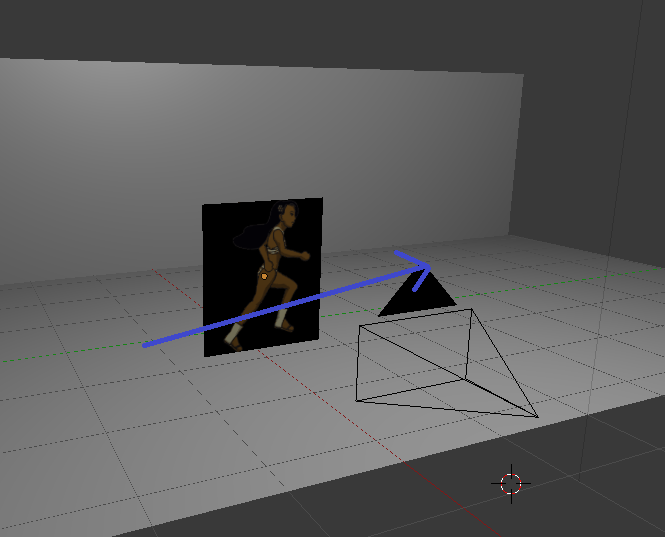
\includegraphics[width=0.7 \textwidth]{05TrabajoRealizado/01DocDiseno02/imagenes/camara01}}
   \subfigure[Seguimiento vertical.]{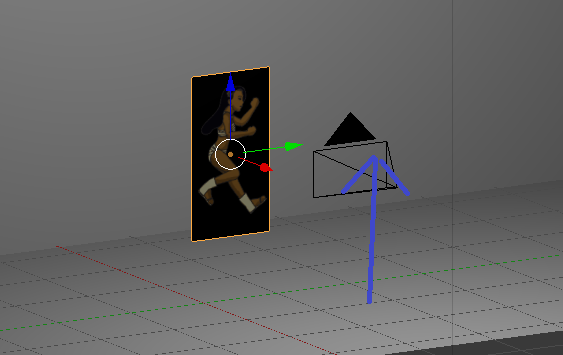
\includegraphics[width=0.7 \textwidth]{05TrabajoRealizado/01DocDiseno02/imagenes/camara02}}
  \caption{La cámara seguirá la posición del jugador en el eje x y y.}
  \label{fig:Camara}
\end{figure} 
 

\par
Por su parte, los controles del juego se establecieron como un conjunto de cuatro 
botones (Ver figura \ref{fig:GUI} ); cada uno con una acción específica a 
desempeñar: mover hacia la izquierda, mover hacia la derecha, disparar, hablar, 
saltar. Siendo periférico o el medio de interacción de los botones y el jugador 
la pantalla táctil del teléfono.  

\begin{figure}
				\centering
				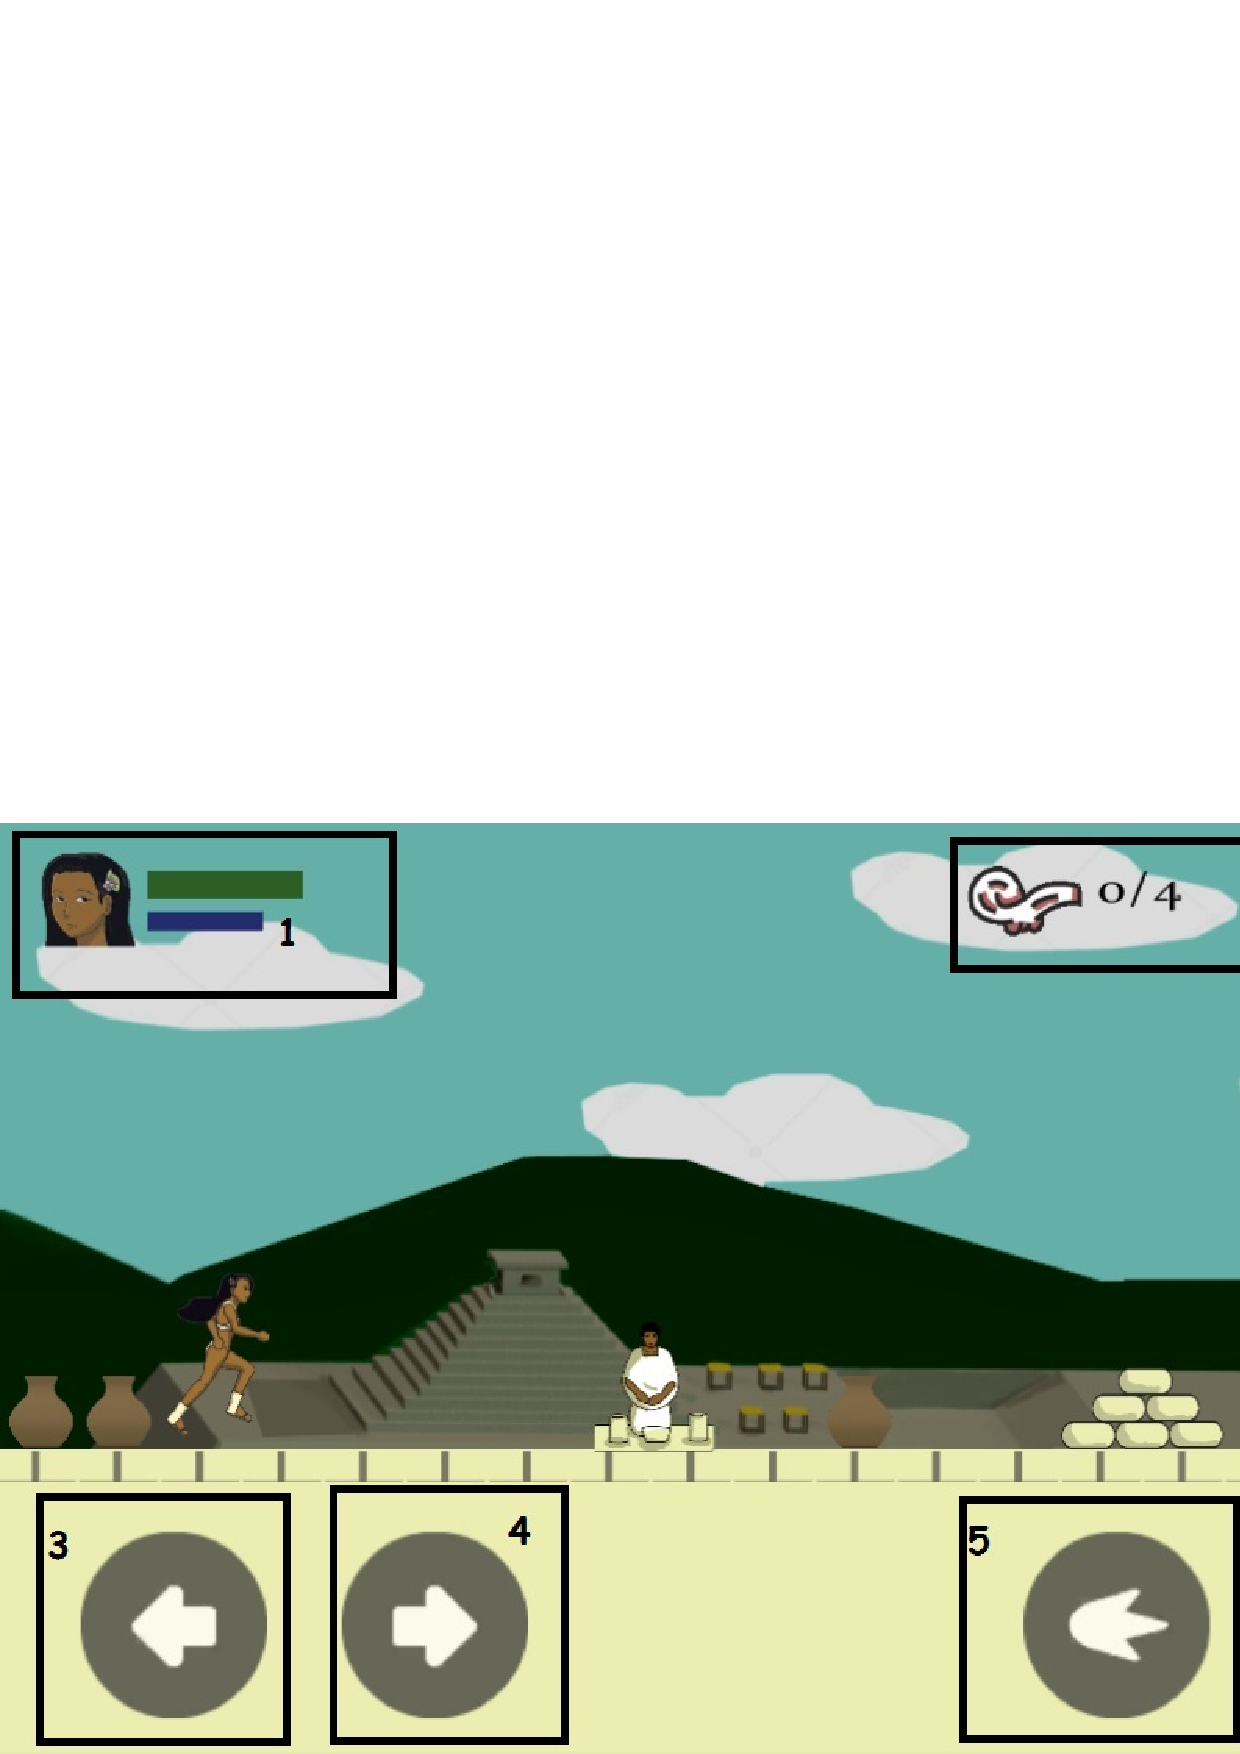
\includegraphics[height=0.3 \textheight]{05TrabajoRealizado/01DocDiseno02/imagenes/ControlCorrerDer}
				\caption{1 Información del personaje jugable, barra verde indicador 
				de la cantidad de vida, barra azul cantidad de tonalli. 2 Objetivos 
				del nivel o información útil. 3 Botón moverse izquierda. 4 Botón 
				moverse derecha. 5 Botón disparar tonalli. 6 Botón saltar.}
				\label{fig:GUI}
\end{figure}


\par
En cuanto al guardado y la carga, se propusieron dos tipos guardado y carga automática 
y guardado y carga de checkpoint; el primero guarda el progreso del jugador al 
completar el nivel y permite inicializar los niveles desbloqueados y el segundo 
se utiliza dentro de un nivel para guardar el progreso del jugador en el nivel 
en caso de que muera pueda iniciar desde el último checkpoint que tocó. 
Si el lector de este documento dese profundizar más en lo anteriormente dicho, 
se le recomienda consultar el Capítulo 5 del documento de diseño.
%===========================================
\subsection{Interfaces}\label{TraReaInterfaces}
Para la navegación dentro del juego, se diseñaron tres interfaces gráficas: 
La pantalla de inicio, Menú principal y el menú de selección de nivel. 
A continuación, se hará una breve descripción de la función principal de 
las interfaces:
\begin{itemize}
	\item\textbf{ Interfaz de inicio:} Presenta el logo del juego y la información 
	legal del mismo, sirve como pantalla de introducción al juego. Conecta con 
	la interfaz de menú principal (Ver figura \ref{fig:PInicio} ) .
	\item \textbf{Interfaz de menú principal:} Muestra la misma ilustración que la 
	pantalla de inicio, con la diferencia de que muestra dos botones en la parte 
	inferior izquierda de la pantalla. Con estos botones se puede empezar una nueva 
	partida o cargar una ya existente. Esta interfaz conecta a la cinemática de 
	inicio del juego si el jugador oprime el botón de empezar partida y confirma 
	que desea empezar una partida nueva o direcciona a la interfaz de menú de 
	selección de nivel, si el jugado oprime el botón de cargar partida y existe 
	un archivo con los datos del juego (Ver figura \ref{fig:PMenuP}).
	\item \textbf{Interfaz de Menú selección de nivel:} En esta interfaz el 
	jugador podrá elegir el nivel que desea jugar, siempre que lo haya desbloqueado 
	con anterioridad (Ver figura \ref{fig:SelNivel}).
\end{itemize}

\begin{figure}
  \centering
   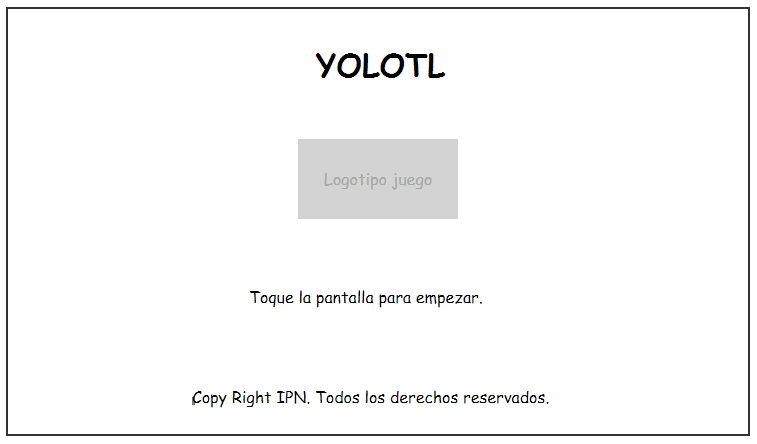
\includegraphics[width=0.6 \textwidth]{05TrabajoRealizado/01DocDiseno02/imagenes/interfaz00}
  \caption{Interfaz 1.0 Pantalla de inicio.}
  \label{fig:PInicio}
\end{figure} 


\begin{figure}
  \centering
   \subfigure[Menú principal] {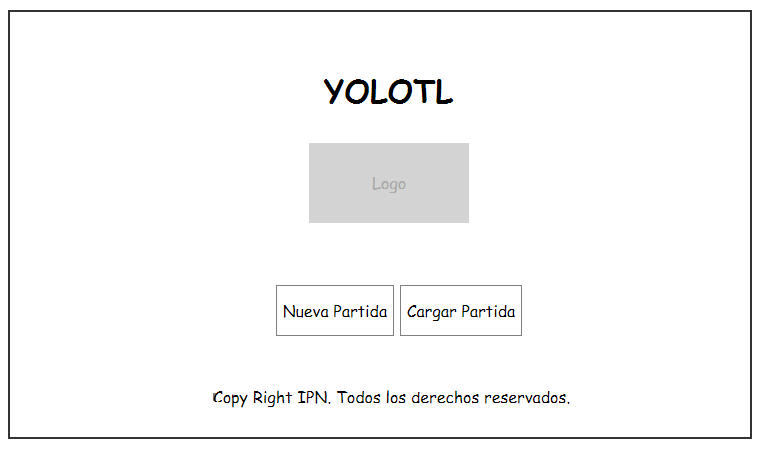
\includegraphics[width=0.6 \textwidth]{05TrabajoRealizado/01DocDiseno02/imagenes/interfaz01}}
   
 	\subfigure[Cuadro de dialogo para confirmar iniciar nueva partida.] {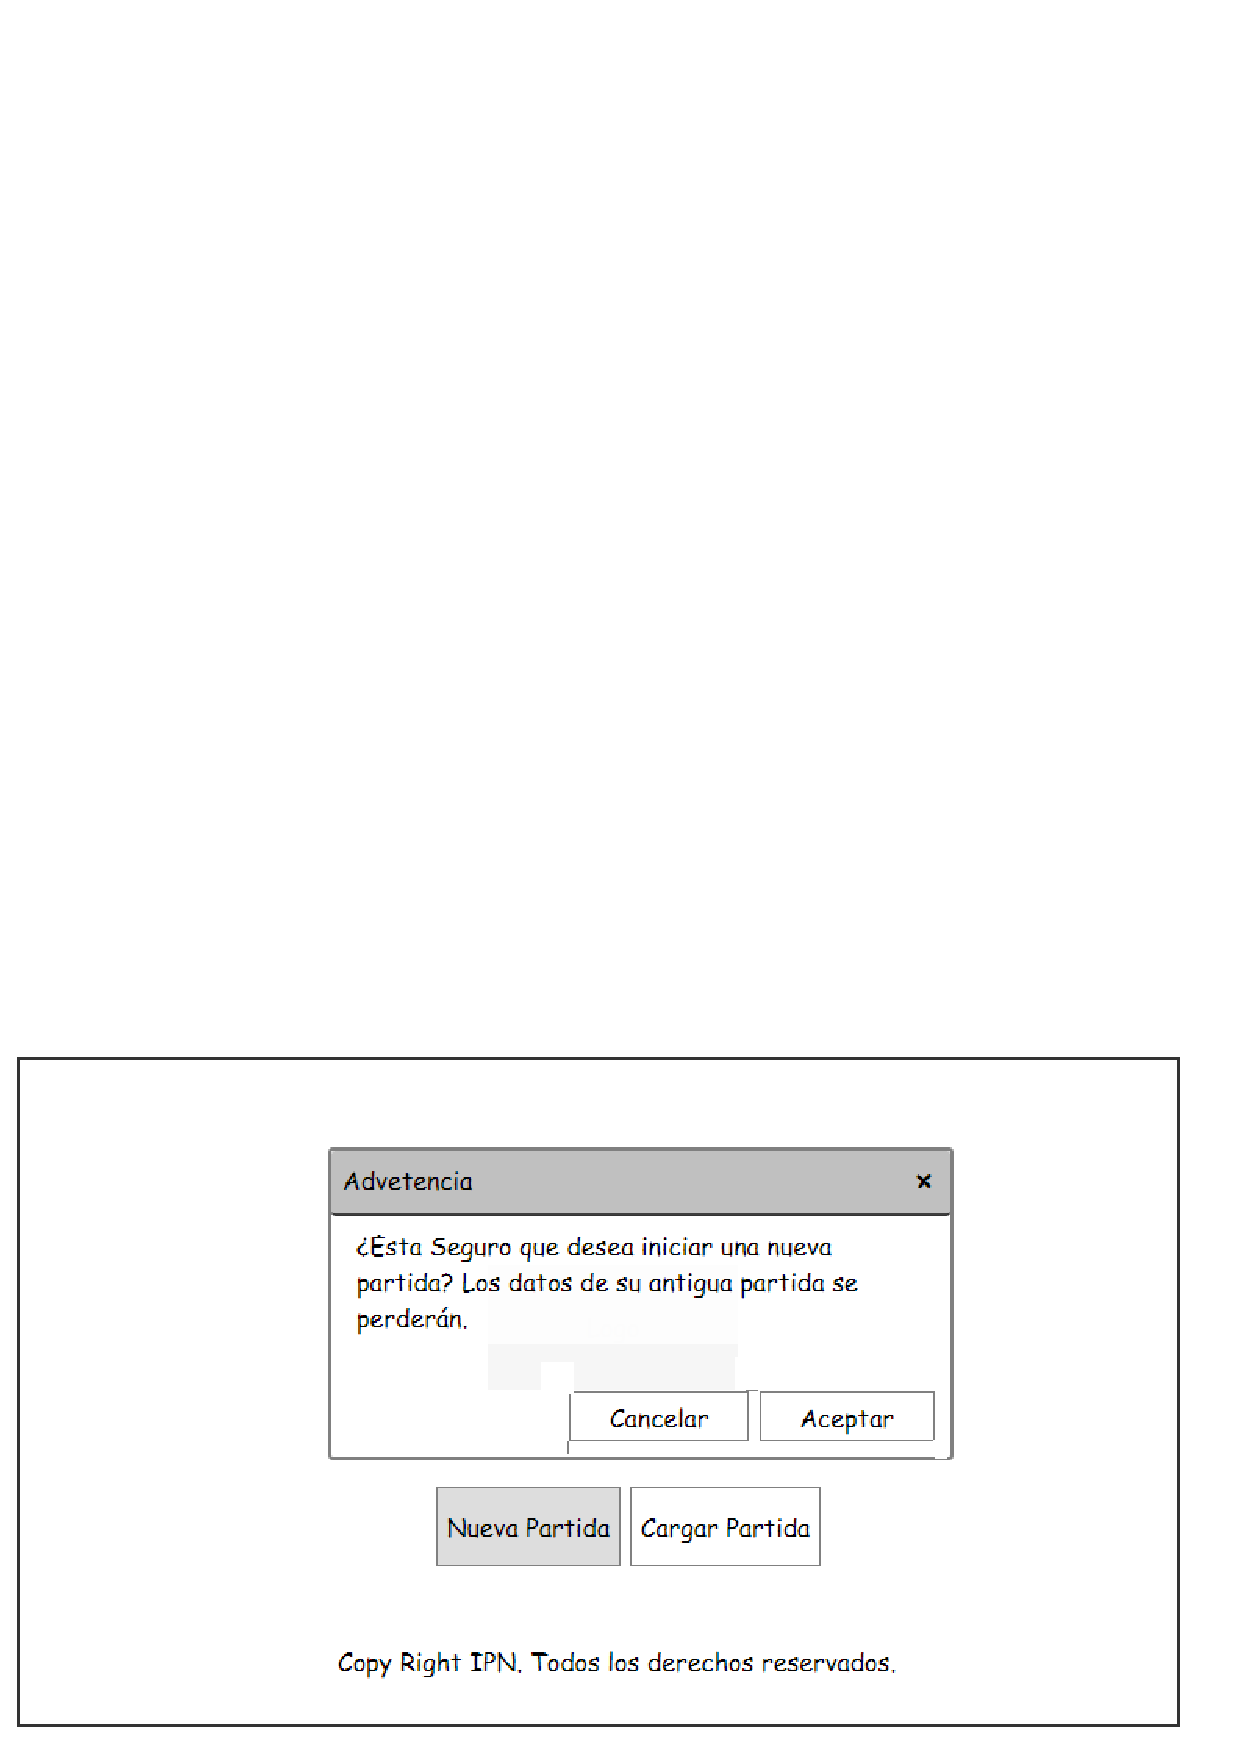
\includegraphics[width=0.6 \textwidth]{05TrabajoRealizado/01DocDiseno02/imagenes/interfaz01_02}}
 	
\subfigure[Cuadro de dialogo cuando no existen partidas que cargar.] {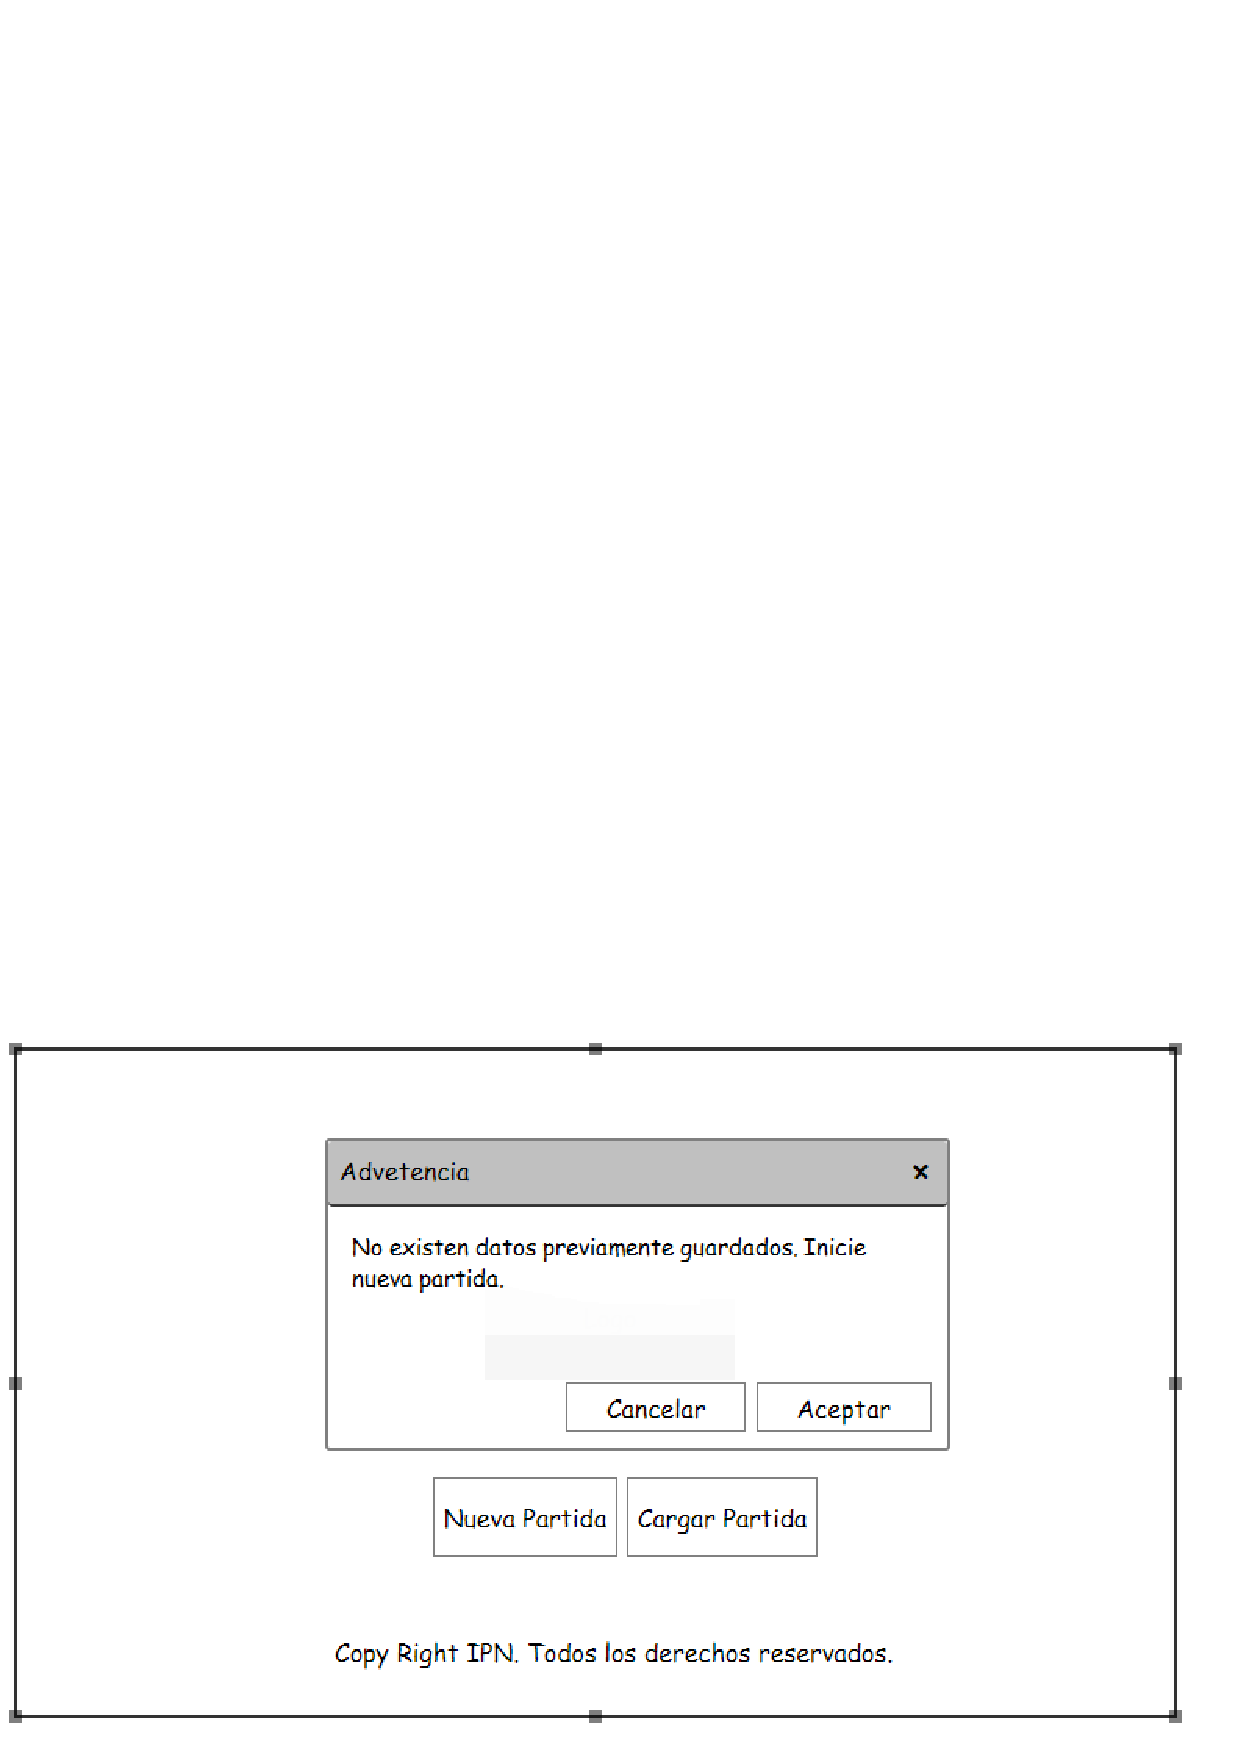
\includegraphics[width=0.6 \textwidth]{05TrabajoRealizado/01DocDiseno02/imagenes/interfaz01_03}}
  \caption{Interfaz 2.00 Menú principal.}
  \label{fig:PMenuP}
\end{figure} 


\begin{figure}
  \centering
   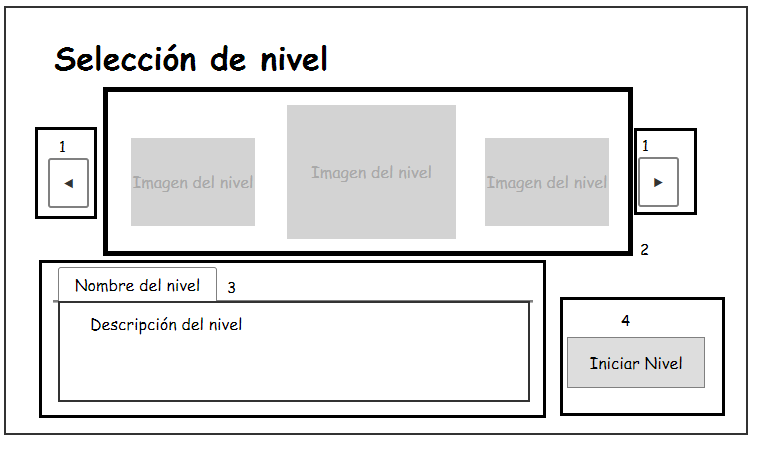
\includegraphics[width=0.6 \textwidth]{05TrabajoRealizado/01DocDiseno02/imagenes/interfaz02_01}
  \caption{Interfaz 2.00 Selección de nivel.1 botones que controlan el carrusel. 2 Carrusel. 3 Información del nivel seleccionado. 4 Botón Iniciar nivel.}
  \label{fig:SelNivel}
\end{figure}  
%===========================================
\subsection{Niveles.} \label{Niveles}
Yolotl es un juego compuesto por diez niveles: un nivel introductorio y los nueve 
niveles del inframundo.  Dado que la idea concepto del juego Yolotl lo situa en 
el Mictlán, la cantidad mínima esperados seria nueve; sin embargo, se tomó la 
decisión de incluir un nivel de introducción debido a los siguientes factores: 

\begin{itemize}
	\item Introducir al jugador a las mecánicas de juego básicas antes de lanzarlo 
	a un nivel más complicado.
	\item Situar el juego dentro de un contexto histórico real, permitiéndole al 
	jugador conocer sobre la sociedad Mexica de una manera en la que el jugador 
	pueda ser participe de este contexto histórico.
	\item Seguir una estructura narrativa básica en la que se presente la vida 
	cotidiana del héroe antes del llamado a la aventura \cite{RefHeroe}.
\end{itemize}

Usualmente, en el juego de Yolotl, un nivel está compuesto de dos secciones: una 
sección de obstáculos y plataformas en donde cumplirá un objetivo propio del nivel 
y otra donde el jugador se enfrentará al enemigo jefe del nivel. A excepción 
del primero y ultimo nivel el resto de los niveles siguen esa estructura. En el 
caso del primer nivel sigue la división de las dos secciones, con la diferencia 
de que no existe un enemigo jefe a vencer en la segunda sección del nivel; 
mientras que en el último nivel existe una única sección en donde el jugador 
se enfrentará a las diferentes transformaciones del jefe final.
\\
\par
La progresión entre niveles es lineal (Ver figura \ref{fig:ProgreNiveles}), 
por lo que no se puede acceder al nivel determinado sin antes haber completado 
a su predecesor; siendo el primer nivel, el que se encuentra disponible de manera 
estándar al empezar una nueva partida. Un nivel se da completado únicamente 
hasta que se ha derrotado al enemigo jefe del nivel; salvo por el primer nivel, 
el cual se considera terminado una vez que el jugador obtiene el arma de la 
protagonista. Cuando el jugador completa un nivel, además de desbloquear el 
siguiente nivel, el jugador podrá ver determinadas cinemáticas con las que podrá 
seguir la historia del juego y obtiene mejoras sobre alguno de los atributos del 
personaje.
\\
\par
En la tabla se encuentra información referente a cada nivel tal como los 
objetivos a cumplir, el enemigo a vencer, lo que se obtiene al completar el nivel.

%%============== PROGRECION DE NIVELES ==============
\begin{figure}
  \centering
   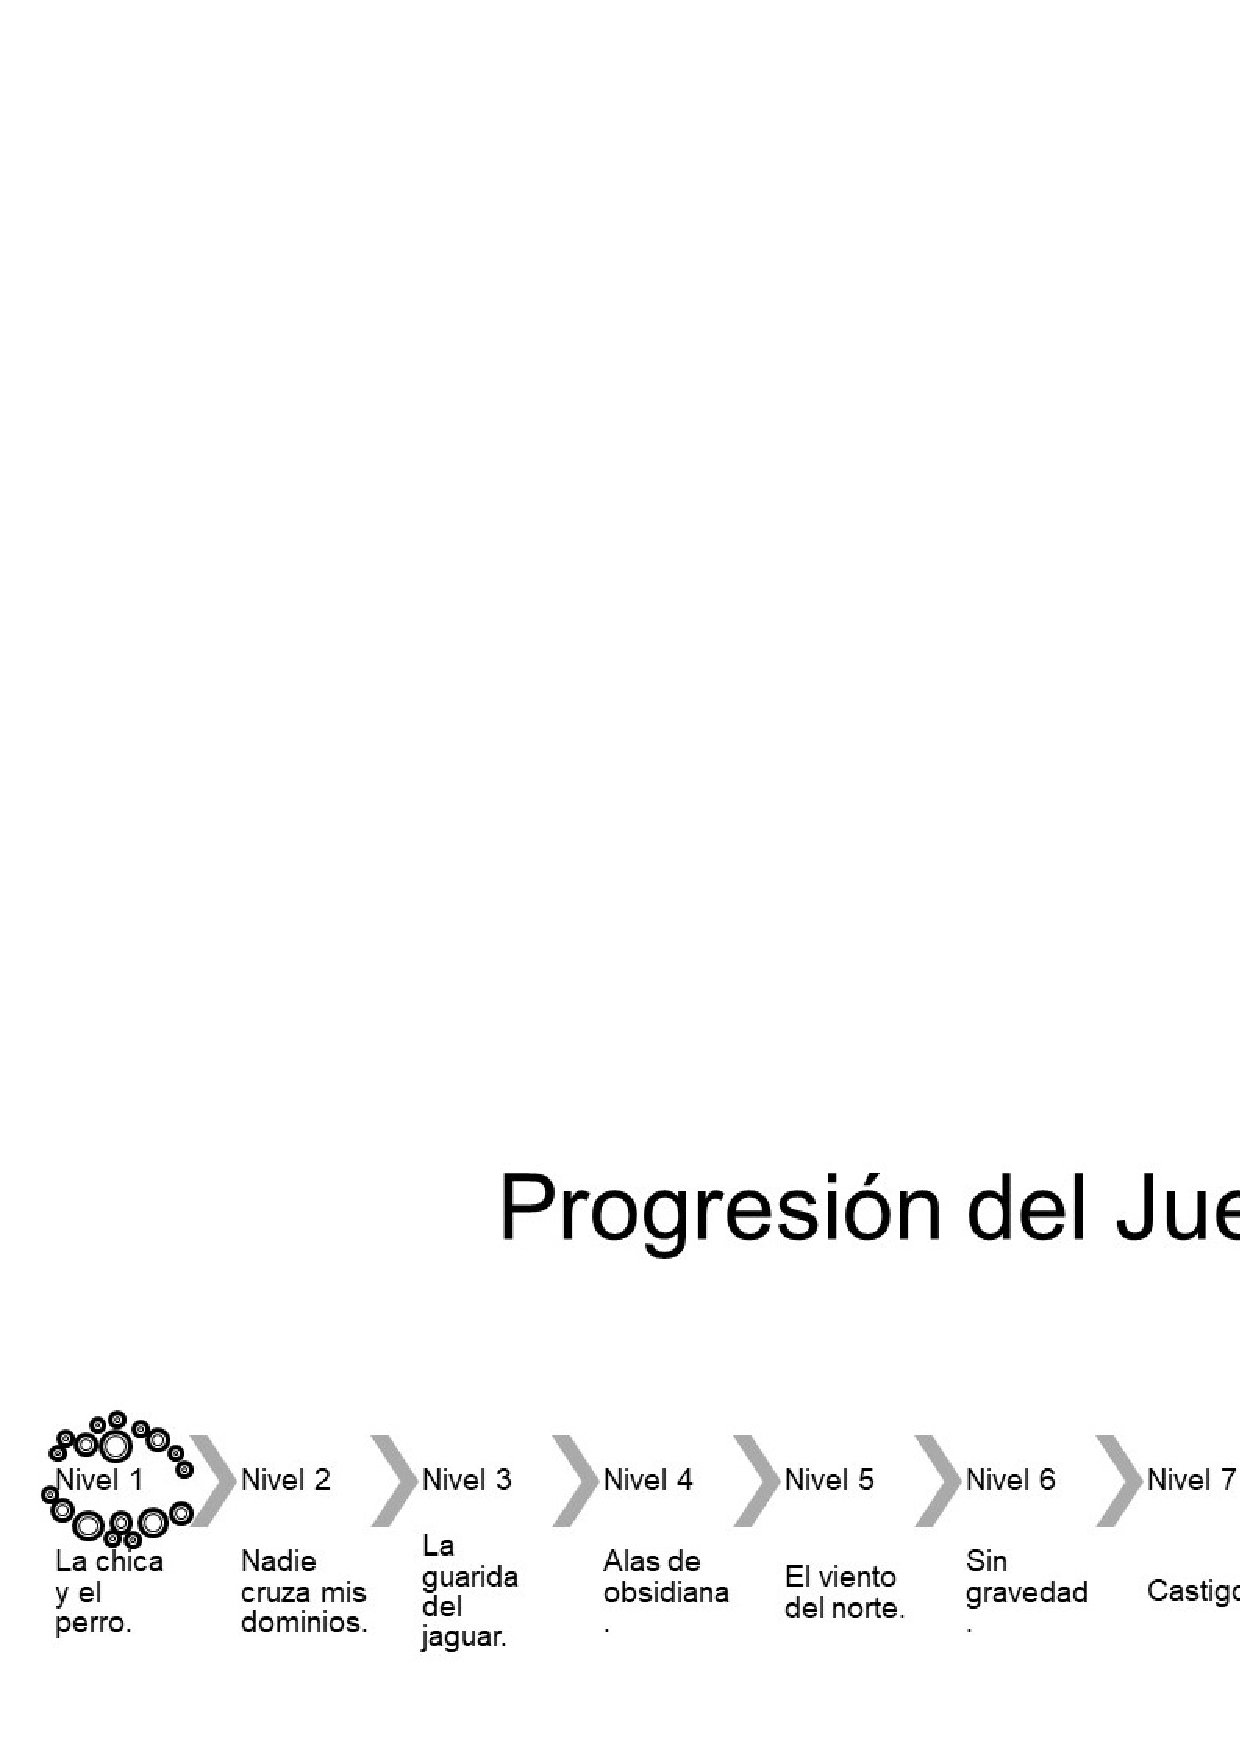
\includegraphics[width=0.8 \textwidth]{05TrabajoRealizado/01DocDiseno02/imagenes/ProgresJuego}
  \caption{Progresión del juego}
  \label{fig:ProgreNiveles}
\end{figure} 

%%============== TABLA DE NIVELES =============
%\begin{table}
	\begin{longtable}[c]{ | m{3.75cm} | m{3.75cm}| m{3.75cm} | m{3.75cm}|} 
		%\endhead		
		%\endfirsthead
		%\endlastfoot
		%\hline
		\rowcolor{cyan} Nivel.& Objetivo & Zona de plataformas	Enemigo jefe & Progreso obtenido. \\ 
		\hline
		%-------------------------------
		Nivel 1 “La chica y el perro”. & 
		Hablar con al menos cuatro ciudadanos.
			\par 
			Interactuar con Xólotl.
			\par 
			Obtener la caracola.&
		Sin enemigo jefe.&
		 Nivel 1.
			\par 
			Cinemática 3.
			\par 
			Cinemática 4.
			\par 
			Habilidad de disparo.		 
		 \\ 
		\hline
		%-------------------------------
		Nivel 2 “Nadie cruza mis dominios”. & 
		Atravesar el rio evitando tocar a los Xoloitzcuintles, por cada Xoloitzcuintles tocado incrementara el poder de Xochitónal. &
		Xochitónal. &
		Mejora en la cantidad de vida de Malinalli.
			\par 
			Cinemática 6.
			\par 
			Cinemática 7.
			\par 
			Cinemática 8.
			\par 
			Cinemática 9.
			\par 
			Cinemática 10.
			\par 
			Nivel 3.		 
		 \\ 
		\hline
		%-------------------------------
		Nivel 3 “La guarida del jaguar”. & 
		Llegar a la guarida de Tepeyóllotl. &
		Tepeyóllotl. &
		Mejora en la cantidad de Tonalli de Malinalli.
			\par 
			Cinemática 12.
			\par
			Cinemática 13.
			\par 
			Cinemática 14.
			\par
			Nivel 4.		 
		 \\ 
		\hline
		%-------------------------------
		Nivel 4 “Alas de obsidiana”. & 
			Encontrar el camino correcto hacia la guarida de Itzpapálotl.
			\par
			Encontrar las tres llaves que abren la puerta de la guarida de Itzpapálotl.&
		Itzpapálotl. &
			 Mejora en la cantidad de vida de Malinalli.
			 \par
			 Cinemática 16.
			 \par
			 Cinemática 17.
			 \par
			 Cinemática 18.
			 \par
			 Cinemática 19.
			 \par
			 Cinemática 20.
			 \par
			 Cinemática 21.
			 \par
			 Cinemática 22.
			 \par
			 Nivel 5.		 
		 \\ 
		\hline
		%-------------------------------
		Nivel 5 “El viento del norte”. & 
		Llegar a la guarida Mictlecayotl.&
		Mictlecayotl. &
		Mejora en la cantidad de Tonalli de Malinalli.
		\par
		Cinemática 24.
		\par
		Cinemática 25.
		\par
		Cinemática 26.
		\par
		Cinemática 27.
		\par
		Nivel 6.		 
		 \\ 
		\hline
		%-------------------------------
		Nivel 6 “Sin gravedad”. & 
		Llegar a la guarida Tlazoltéotl &
		Tlazoltéotl. &
		Mejora en la cantidad de vida de Malinalli.
		\par
		Cinemática 29.
		\par
		Cinemática 30.
		\par
		Cinemática 31.
		\par
		 Nivel 7.		 
		 \\ 
		\hline
		%-------------------------------
		Nivel 7 “Castigo”. & 
		Llegar a la guardia Itztlacoliuhqui. &
		Itztlacoliuhqui. &
		Mejora en la cantidad de Tonalli de Malinalli.
		\par
		Cinemática 33.
		\par
		Cinemática 34.
		\par
		Cinemática 35.
		\par
		Nivel 8.		 
		 \\ 
		\hline
		%-------------------------------
		Nivel 8 “La última batalla del jaguar”. & 
		Llegar a la guarida de Tepeyóllotl.&
		Tepeyóllotl. &
		Mejora en la cantidad de vida de Malinalli.
		\par		
		Cinemática 37.
		\par
		Cinemática 38.
		\par
		Cinemática 39.
		\par
		Nivel 9.		 
		 \\ 
		\hline
		%-------------------------------
		Nivel 9 “El último caballero del rey”. & 
		Superar la zona de Tula.
		\par
		Superar la zona de Oluta.&
		Nexoxcho. &
		Mejora en la cantidad de Tonalli de Malinalli.
		\par		
		Cinemática 44.
		\par
		Cinemática 45.
		\par
		Cinemática 46.
		\par
		Nivel 10. 
		 \\ 
		\hline
		%-------------------------------
		Nivel 10 “El rey del Mictlán”. & 
		Sin objetivos &
		Mictlantecutli. &
		Cinemática 47.
		\par		
		Juego terminado. 
		 \\ 
		\hline
	\end{longtable}

	%\caption{Información de los niveles.}
	%\label{Tab:Niveles}
%\end{table}
%===========================================
\subsection{Obstáculos}
De manera particular, para el proyecto Yolotl, se entiende por obstáculos a aquellos objetos dentro de un nivel que dificultan el avance continuo del jugado o que faciliten el fallo del jugador.
\\
\par
A diferencia de los personajes, la metodología huddle no maneja una plantilla para documentar estos objetos, por lo que se propuso una plantilla propia. Los campos de la plantilla son:
	\begin{itemize}
		\item Nombre del obstáculo.
		\item Descripción: Este campo describe tanto físicamente el objeto como su comportamiento e interacción con el jugador. 
		\item Esquema: Imagen de apoyo que facilita la comprensión de la descripción. 
	\end{itemize}
En total se definieron alrededor de 11 obstáculos, mismos que se podrán encontrar repartidos a lo largo de los niveles del juego. Algunos obstáculos serán exclusivos de un nivel mientras que otros se podrán encontrar en todos los niveles.
 \\
 \par
 A continuación se listarán los obstáculos del juego:
 	\begin{itemize}
 		\item Caja.
 		\item Sacos de cacao.
 		\item Plataforma móvil.
 		\item Plataforma que cae.
 		\item Plataforma que desaparece.
 		\item Estalagmitas.
 		\item Viento temporal.
 		\item Piedras filosas.
 		\item Piso congelado.
 		\item Bolas de nieve.
 		\item Lluvia de flechas.
 	\end{itemize}
%===========================================
\subsection{Ambientación}
	Para garantizar la inmersión del jugador, el videojuego se vale de diferentes
	 elementos multimedia. Estos elementos son la música de fondo (BGM, pos sus 
	 siglas en inglés), los efectos de sonido (SFX, por sus siglas en inglés) y  
	 efectos espaciales (FX, por su siglas en inglés).
\\
\par	
	Huddle maneja un aparatado para incluir este tipo de elementos dentro de la 
	documentación del juego; sin embargo, no incluye ninguna guía sobre como debería 
	de redactarse las descripciones de BGM y SFX; en consecuencia estos elementos 
	fueron documentados escribiendo el nombre de sonido o música, seguido de una 
	breve descripción del mismo.   
\\
\par
Durante la redacción de este aparatado se detectó que existían dos secciones para 
documentar BGM y SFX, con la diferencia de que en una los términos se encontraban 
escritos en sus siglas en inglés y en el otro apartado se encontraba en español, 
por lo que se eliminó el apartado en español. Luego de que se detectara esta 
duplicación de apartados, se descubrió que no existía ningún apartado para documentar 
los FX, seguido de esto se creo dicho apartado. En cuanto a la documentación de FX, 
se siguió la misma estructura que con BGM y SFX: escribir el nombre de FX y 
describirlo para dar una idea de como se vería en el nivel y bajo que interacciones 
se activaría. 
%===========================================
\subsection{Argumento del videojuego}
Huddle maneja un apartado llamado \textbf{Guión} para documentar de manera detallada 
la historia del videojuego. No obstante, al igual que como sucede con algunos de 
los apartados ya descritos, Huddle no proporciona una plantilla para documentarlo. 
Ante la falta de una plantilla para documentar el argumento y ante la existencia 
de cinemáticas dentro de los niveles y fuera de estos, se decidió que el argumento 
del juego se documentaría como una animación. Contando así con tres guiones:
	\begin{itemize}
		\item \textbf{Guión literario}:Este guión es parecido a un guión teatral. 
		Por medio de escenas va desarrollando la historia, mostrando la secuencia 
		de diálogos que entablan los personajes participes en el argumento. Para 
		el caso particular del videojuego Yolotl, las escenas recibe el nombre de 
		cinemáticas. Cada cinemática se documentara bajo la siguiente plantilla:
			\begin{itemize}
				\item Numero de la cinemática seguido del nombre la locación donde 
				acontece ésta; en caso de que la escena suceda en el interior de 
				alguna edificación se pondrá seguido del nombre de la locación el 
				prefijo int, en caso de suceder en el exterior se colocará el 
				prefijo ext.
				\item Relación con los nombres de todos los personajes que participan 
				en la escena.
				\item Breve descripción de la locación.
				\item Secuencia de diálogos. Cada diálogo va precedido por el nombre 
				de personaje que lo dice, el nombre del personaje debe de ir en 
				mayúsculas y subrayado. 
			\end{itemize}
			\item Storyboard: El storyboard es una secuencia de imágenes que narran 
			de manera visual la historia. Cada imagen va comentada de tecnicismos 
			que faciliten la descripción de acciones (tales como el desplazamiento 
			de la cámara, movimientos de personajes, intención del personaje en 
			decir un diálogo, etc.) \cite{RefStoyBoard}.  			 
	\end{itemize}


	\section{Análisis del juego}
En esta sección se presenta el analisis que se realizo del juego con base en el 
documento de diseño descrito en el apartado \ref{docDisenio}.Primeramente se 
describe al usuario que se identificó y las acciones que éste puede realizar 
dentro del juego; en segundo lugar se habla de las clases que componen el juego, 
describiéndose lo tres tipos de clases en el que se clasificaron, para 
posteriormente listar que clases pertenecen a cada un de los tipos. Para finalizar 
esta sección se describe la comunicación entre clases para tres procesos que 
realiza el juego. 

	\subsection{Usuario del sistema}
	Tomando como referencia el documento de diseño se identificó el siguiente actor:
	\begin{itemize}
		\item \textbf{Jugador:} Es el usuario del sistema y quien interactua con
		el mismo. Dentro del sistema el jugador puede: 
			\begin{itemize}
				\item Empezar una partida nueva.	
				\item Cargar una partida ya existente.
				\item Elegir un nivel para jugar.  
				\item Jugar.
				\item Pausar Nivel.
				\item Reanudar nivel pausado.
				\item Ver cinemática.
			\end{itemize}			   
	\end{itemize}	
	
	\subsection{Clases del juegos} \label{ClasesJuego}
	A partir del documento de diseño se identificaron al rededor de (); estas 
	clases se dividen en tres grupos:
		\begin{itemize}
			\item \textbf{Controladores:} Clases encargadas de controlar la gestión de 
			la partida y la navegación dentro del juego. Estas clases regulan las acciones 
			de las clases actoras y desencadenan determinados eventos dentro del juego
			dependiendo de las acciones del Jugador y de las reglas de los niveles.
			
			\item \textbf{Actores:} Son las clases que modelan a los enemigos, obstáculos,
			\textit{checkpoints} y el jugador.
			 
			 \item \textbf{Auxiliares:} Son todas aquellas clases que ayudan a los controladores
			 a cumplir con su funcionalidad al permitirle a los controladores obtener datos 
			 para inicializar valores o garantizar las transiciones entre interfaces.
		\end{itemize}
		
	\subsubsection{Clases controladoras} \label{ClaseCtrl}
		\begin{itemize}
			\item \textbf{PrincipalMenuCtrl:} Esta clase se encarga de la funcionalidad del menú 
			principal. Esta clase esta a cargo de:
			\begin{itemize}
				\item Empezar nueva partida.
				\item Cargar nueva partida.
				\item Mostrar mensajes de confirmación antes de proceder con cambios 
				irreversibles a los datos de partida.
				\item Mostrar mensaje de aviso en caso de no encontrar exista una partida 
				guardada. 
			\end{itemize}
			%=======================================
			\item \textbf{SelectLevelMenu:} Esta clase controla la funcionalidad del menú de 
			selección nivel. Esta clase realiza:
			\begin{itemize}
				\item Habilitar solo los niveles y cinemáticas que el jugador haya 
				desbloqueado.
				\item No permitir que el jugador pueda acceder a niveles o cinemáticas 
				que el jugador no haya desbloqueado.
				\item Direccionar al jugador al nivel o a la cinemática que seleccionó.
			\end{itemize}
			%=======================================
			\item \textbf{GameDataCtrl:} Esta clase controla el archivo de los datos de 
			partida, este archivo sera de formato binario, este formato es un tipo de 
			archivo que propio de Unity y permite proteger los datos de las partidas evitando
			que estos puedan ser modificados por el jugador, garantizando así la integridad 
			de la información. Está ligada a la mayoría de los controladores pues de ella depende 
			 guardar y cargar el progreso del jugador para inicializar valores como: la 
			 vida del jugador, su cantidad de \textit{Tonalli}, los niveles disponibles, etc. 
			 Dentro de su funcionalidad está: 
			\begin{itemize}
				\item Verificar la existencia del archivo de datos de partida.
				\item Crear un archivo de datos de partida.
				\item Leer los datos del archivo de datos de partida.
				\item Escribir datos en el archivo de partida.
			\end{itemize}
			%=======================================
			\item \textbf{DialogueCtrl:} Esta clase se encarga del despliegue de diálogos
			en las cinemáticas y dentro de los niveles. Esta clase realiza las siguientes 
			actividades:
			\begin{itemize}
				\item Iniciar el despliegue de diálogos.
				\item Mostrar el dialogo siguiente.
				\item Finalizar el despliegue diálogos. 
			\end{itemize}	
			%=======================================
			\item \textbf{TalkedCharactersCtrl:} Esta clase asigna una instancia de la 
			clase \textit{Dialogue} a cada una de las instancias de la clase 
			\textit{TalkedCharacter}.
			%=======================================
			\item \textbf{CutsceneCtrl:} Esta clase se encarga de vincular el despliegue 
			de diálogos con las animaciones de las cinemáticas. Esta clase tiene diversas 
			clases hijas que heredan su funcionalidad de vinculación de diálogos y animación 
			incorporando las consideraciones necesarias para el control de cada cinemática.
			%=======================================
			\item \textbf{AudioCtrl:} Esta clase esta a a cargo de generar los sonidos de \textit{SFX} 
			dentro del juego utilizando la posición del jugador o de los enemigos. 
			%=======================================
			\item \textbf{LevelCtrl:} Esta clase controla el nivel que el jugador esta 
			jugando. Esta clase realiza las siguientes acciones:
			\begin{itemize}
				\item Inicializar los atributos de la clase \textit{Player}.
				\item Verificar que el jugador este vivo.
				\item Actualizar la barra de vida del jugador.
				\item Actualizar la barra de cantidad \textit{Tonalli}.
				\item Pausar el juego.
				\item Reanudar juego pausado. 
			\end{itemize}
			Esta clase tiene clases hijas que se encargan de:
				\begin{itemize}
					\item Verificar que se cumplan los objetivos específicos del nivel.
					\item Actualizar los objetivos del nivel.
					\item Actualizar los contadores de los objetivos.
					\item Guardar el progreso obtenido en el nivel.
					\item Inicializar los valores del jugador con base al \textit{checkpoint} activo. 
				\end{itemize}
			%=======================================
			\item \textbf{CameraCtrl:} Esta clase controla el desplazamiento de la cámara.
			%=======================================
			\item \textbf{MobileUICtrl:} Esta clase se encarga de comunicar al jugador 
			con la clase \textit{Player}. Es a través de esta clase que el jugador puede controlar 
			al personaje jugable. Esta clase le permite al jugador:
			\begin{itemize}
				\item Mover al personaje jugable a la derecha.
				\item Mover al personaje a la izquierda.
				\item Detener el movimiento del jugador.
				\item Actualizar la barra de cantidad \textit{Tonalli}.
				\item Pausar el juego.
				\item Reanudar juego pausado. 
			\end{itemize}
			%=======================================
			\item \textbf{ArrowCreator:} Esta clase crea objetos que instancían al prefab "Arrow".								
		\end{itemize}				  
	\subsubsection{Clases Actores}
A continuación se listan las clases actores: 
		\begin{itemize}
			\item \textbf{Player:} Esta clase se encarga de las acciones del personaje 
			jugable, actualizar sus estados y gestionar el valor de sus atributos. 
			Esta clase esta a cargo de:
			\begin{itemize}
				\item Mover al personaje jugable de manera horizontal.
				\item Controlar la maquina de estados de las animaciones del personaje 
				jugable.
				\item Detectar las colisiones del personaje jugable.
				\item Actualizar la cantidad de vida al recibir daño.
				\item Realizar disparo de \textit{Tonalli}.
				\item Actualizar la cantidad de \textit{Tonalli} al efectuar un disparo.  
				\item Saltar. 
			\end{itemize}
			%=======================================
			\item \textbf{TalkedCharacter:} Esta clase modela el funcionamiento de un
			ciudadano con el que el jugador debe interactuar en el nivel 1.
			Esta clase esta a cargo de:
			\begin{itemize}
				\item Mostrar un ícono de diálogo para indicarle al jugador que debe de 
				interactuar con éste.
				\item Ocultar el ícono de diálogo.
				\item Indicarle a la clase DialogueCtrl que se inicia un diálogo.  
			\end{itemize}
			%=======================================
			\item \textbf{DroppingPlatform:} Esta clase modela el funcionamiento 
			del obstáculo Plataforma que cae, por lo que al hacer contacto con un objeto de 
			la clase \textit{GroundCollisionCtrl} el objeto que instancie esta clase 
			empezará a caer despues de \textit{n} segundos. 
			%=======================================
			\item \textbf{MovingPlatform:} Esta clase modela el funcionamiento 
			del obstáculo Plataforma que móvil. Haciendo uso de dos posiciones: A y B, el 
			objeto que instancia esta clase se mueve de manera cíclica de la posición A a 
			la B y de la B a la A. 
			%=======================================
			\item \textbf{DisappearingPlatform:} Esta clase modela el funcionamiento 
			del obstáculo Plataforma que desaparece, esta clase hace que el objeto que la 
			instancie aparezca y desaparezca de manera cíclica, activando y desactivando 
			los colisionadores del objeto. 
			%=======================================
			\item \textbf{Stalagmite:} Esta clase modela el comportamiento del obstáculo 
			estalagmita. Esta clase hace que el objeto que la instancie caiga cuando 
			detecte que el jugador se posiciona por debajo de este objeto.    
			%=======================================
			\item \textbf{PushingObstacle:} Esta clase modela el comportamiento de dos 
			obstáculos: viento temporal y bolas de nieve. Haciendo uso de una posición, la
			clase determina hacia que dirección debe de incrementar su dimensión y el tamaño 
			de su colisionador.      
			%=======================================	
			\item \textbf{Arrow:} Clase que produce un movimiento vertical descendente al 
			objeto que la instancia.   
			%=======================================
			\item \textbf{\textit{Enemy}:} Esta clase modela el comportamiento común que 
			tienen los enemigos de tipo normal y los de tipo jefe. De esta clase heredan 
			su funcionamiento las clase \textit{NormalEnemy} y \textit{BossEnemy}.Esta 
			clase se encarga de:  
			\begin{itemize}
				\item Controlar las transiciones de la maquina de estados que controla las 
				animaciones del enemigo.
				\item Gestiona la detección de colisiones del enemigo.
				\item Actualizar la cantidad de vida del Enemigo.
			\end{itemize}
			%=======================================
			\item \textbf{\textit{NormalEnemy}:} Esta clase modela el comportamiento común que 
			tienen los enemigos de tipo normal. Esta clase hereda su funcionamiento de la clase
			 \textit{Enemy}. La clase NormalEnemy hereda su funcionalidad a las clases 
			\textit{ Jaguar, Bird, Armadillo, PurpleGost} y \textit{RedGost}.Esta 
			clase se encarga de:  
			\begin{itemize}
				\item Controlar el patrón de movimiento de los enemigos de tipo 
				normal.
				\item  Verificar la cercanía que tiene el enemigo normal con otros objetos, 
				obstáculos y enemigos para ajustar su rango de acción y evitar que interfiera con el 
				funcionamiento de otro objeto.
			\end{itemize}					
			%=======================================
			\item \textbf{\textit{Jaguar}:} Esta clase modela el comportamiento del enemigo jaguar 
			(Consultar la ficha de personaje en la Sección de personajes en el documento de diseño). 
			Esta clase hereda su funcionamiento de la clase \textit{NormalEnemy}. Esta 
			clase se encarga de:  
			\begin{itemize}
				\item Sincronizar el desplazamiento del jaguar con su maquina de estados para que modele
				el patrón de ataque del jaguar. 
			\end{itemize}
			%=======================================
			\item \textbf{\textit{Bird}:} Esta clase modela el comportamiento de dos personajes de tipo
			normal: Chara enana y Zopilote (Consultar la ficha de personaje en la Sección de personajes en 
			el documento de diseño). Esta clase hereda su funcionamiento de la clase 
			\textit{NormalEnemy}. Esta clase se encarga de:  
			\begin{itemize}
				\item Sincronizar el desplazamiento del ave con su maquina de estados para que modele
				el patrón de ataque de Chara enana y del zopilote. 
			\end{itemize}
			%=======================================
			\item \textbf{\textit{Armadillo}:} Esta clase modela el comportamiento del personaje 
			armadillo (Consultar la ficha de personaje en la Sección de personajes en 
			el documento de diseño). Esta clase hereda su funcionamiento de la clase 
			\textit{NormalEnemy}. Esta clase se encarga de:  
			\begin{itemize}
				\item Sincronizar el desplazamiento del jaguar con su maquina de estados para que modele
				el patrón de ataque del armadillo. 
			\end{itemize}
			%=======================================
			\item \textbf{\textit{PurpleGost}:} Esta clase modela el comportamiento del personaje 
			fantasma purpura (Consultar la ficha de personaje en la Sección de personajes en 
			el documento de diseño). Esta clase hereda su funcionamiento de la clase 
			\textit{NormalEnemy}. Esta clase se encarga de:  
			\begin{itemize}
				\item Sincronizar el desplazamiento del jaguar con su maquina de estados para que modele
				el patrón de ataque del fantasma purpura. 
			\end{itemize}
			
			%=======================================
			\item \textbf{\textit{RedGost}:} Esta clase modela el comportamiento del personaje 
			fantasma rojo (Consultar la ficha de personaje en la Sección de personajes en 
			el documento de diseño). Esta clase hereda su funcionamiento de la clase 
			\textit{NormalEnemy}. Esta clase se encarga de:  
			\begin{itemize}
				\item Sincronizar el desplazamiento del jaguar con su maquina de estados para que modele
				el patrón de ataque del fantasma rojo.
				\item Instanciar el objeto ShootEnemy. 
			\end{itemize}
			%=======================================
			\item \textbf{\textit{BossEnemy}:} Esta clase modela el comportamiento común que 
			tienen los enemigos de tipo ¿jefe. Esta clase hereda su funcionamiento de 
			la clase \textit{Enemy}. La clase BosslEnemy hereda su funcionalidad a las clases 
			\textit{ Xochitonal, Tepeyollotl,Itzpapalotl, Mictlecayotl, Tlazolteotl, 
			Itztlacoliuhqui, Nexoxcho, MictlantecutliPhase01, MictlantecutliPhase02} 
			y \textit{MictlantecutliPhase03}.Esta clase se encarga de:  
			\begin{itemize}
				\item Controlar el patrón de movimiento de los enemigos de tipo 
				jefe.
				\item  Verificar la cercanía que tiene el enemigo tipo jefe con el jugador 
				y con los limites del escenario.
			\end{itemize}	
			%=======================================
			\item \textbf{\textit{Xochitonal}:} Esta clase modela el comportamiento del personaje 
			\textit{Xochitónal} (Consultar la ficha de personaje en la Sección de personajes en 
			el documento de diseño). Esta clase hereda su funcionamiento de la clase 
			\textit{BossEnemy}. Esta clase se encarga de:  
			\begin{itemize}
				\item Sincronizar el desplazamiento del \textit{Xochitónal} con su maquina 
				de estados para que modele el patrón de \textit{Xochitónal}.
				\item Toma decisiones en cuanto a los ataques a realizar basándose en su 
				nivel de vida.
			\end{itemize}
			%=======================================
			\item \textbf{\textit{Tepeyollotl}:} Esta clase modela el comportamiento del personaje 
			\textit{Tepeyóllotl} (Consultar la ficha de personaje en la Sección de personajes en 
			el documento de diseño). Esta clase hereda su funcionamiento de la clase 
			\textit{BossEnemy}. Esta clase se encarga de:  
			\begin{itemize}
				\item Sincronizar el desplazamiento del \textit{Tepeyóllotl} con su maquina 
				de estados para que modele el patrón de \textit{Tepeyóllotl}.
				\item Toma decisiones en cuanto a los ataques a realizar basándose en su 
				nivel de vida.
			\end{itemize}
			%=======================================
			\item \textbf{\textit{Itzpapalotl}:} Esta clase modela el comportamiento del personaje 
			\textit{Itzpápalotl} (Consultar la ficha de personaje en la Sección de personajes en 
			el documento de diseño). Esta clase hereda su funcionamiento de la clase 
			\textit{BossEnemy}. Esta clase se encarga de:  
			\begin{itemize}
				\item Sincronizar el desplazamiento del \textit{Itzpápalotl} con su maquina 
				de estados para que modele el patrón de \textit{Itzpápalotl}.
				\item Toma decisiones en cuanto a los ataques a realizar basándose en su 
				nivel de vida.
			\end{itemize}
			%=======================================
			\item \textbf{\textit{Mictlecayotl}:} Esta clase modela el comportamiento del personaje 
			\textit{Mictlecayotl} (Consultar la ficha de personaje en la Sección de personajes en 
			el documento de diseño). Esta clase hereda su funcionamiento de la clase 
			\textit{BossEnemy}. Esta clase se encarga de:  
			\begin{itemize}
				\item Sincronizar el desplazamiento del \textit{Mictlecayotl} con su máquina 
				de estados para que modele el patrón de \textit{Mictlecayotl}.
				\item Toma decisiones en cuanto a los ataques a realizar basándose en su 
				nivel de vida.
			\end{itemize}
			%=======================================
			\item \textbf{\textit{Tlazolteotl}:} Esta clase modela el comportamiento del personaje 
			\textit{Tlazoltéotl} (Consultar la ficha de personaje en la Sección de personajes en 
			el documento de diseño). Esta clase hereda su funcionamiento de la clase 
			\textit{BossEnemy}. Esta clase se encarga de:  
			\begin{itemize}
				\item Sincronizar el desplazamiento del \textit{Tlazoltéotl} con su maquina 
				de estados para que modele el patrón de \textit{Tlazoltéotl}.
				\item Toma decisiones en cuanto a los ataques a realizar basándose en su 
				nivel de vida.
			\end{itemize}
			%=======================================
			\item \textbf{\textit{Itztlacoliuhqui}:} Esta clase modela el comportamiento del personaje 
			\textit{Itztlacoliuhqui} (Consultar la ficha de personaje en la Sección de personajes en 
			el documento de diseño). Esta clase hereda su funcionamiento de la clase 
			\textit{BossEnemy}. Esta clase se encarga de:  
			\begin{itemize}
				\item Sincronizar el desplazamiento del \textit{Itztlacoliuhqui} con su máquina 
				de estados para que modele el patrón de \textit{Itztlacoliuhqui}.
				\item Toma decisiones en cuanto a los ataques a realizar basándose en su 
				nivel de vida.
			\end{itemize}
			%=======================================
			\item \textbf{\textit{Nexoxcho}:} Esta clase modela el comportamiento del personaje 
			\textit{Nexoxcho} (Consultar la ficha de personaje en la Sección de personajes en 
			el documento de diseño). Esta clase hereda su funcionamiento de la clase 
			\textit{BossEnemy}. Esta clase se encarga de:  
			\begin{itemize}
				\item Sincronizar el desplazamiento del \textit{Nexoxcho} con su maquina 
				de estados para que modele el patrón de \textit{Nexoxcho}.
				\item Toma decisiones en cuanto a los ataques a realizar basándose en su 
				nivel de vida.
			\end{itemize}
			%=======================================
			\item \textbf{\textit{MictlantecutliPhase01}:} Esta clase modela el 
			comportamiento del personaje \textit{Mictlantecutli} (Consultar la ficha 
			del personaje en la Sección de personajes en 
			el documento de diseño). Esta clase hereda su funcionamiento de la clase 
			\textit{BossEnemy}. Esta clase se encarga de:  
			\begin{itemize}
				\item Sincronizar el desplazamiento del \textit{Mictlantecutli} con su máquina 
				de estados para que modele el patrón de \textit{Mictlantecutli}.
				\item Toma decisiones en cuanto a los ataques a realizar basándose en su 
				nivel de vida.
			\end{itemize}
			%=======================================
			\item \textbf{\textit{MictlantecutliPhase02}:} Esta clase modela el 
			comportamiento del personaje \textit{Mictlantecutli} (Consultar la ficha 
			del personaje en la Sección de personajes en 
			el documento de diseño). Esta clase hereda su funcionamiento de la clase 
			\textit{BossEnemy}. Esta clase se encarga de:  
			\begin{itemize}
				\item Sincronizar el desplazamiento del \textit{Mictlantecutli} con su maquina 
				de estados para que modele el patrón de \textit{Mictlantecutli}.
				\item Toma decisiones en cuanto a los ataques a realizar basándose en su 
				nivel de vida.
			\end{itemize}
			%=======================================
			\item \textbf{\textit{MictlantecutliPhase03}:} Esta clase modela el 
			comportamiento del personaje \textit{Mictlantecutli} (Consultar la ficha 
			del personaje en la Sección de personajes en 
			el documento de diseño). Esta clase hereda su funcionamiento de la clase 
			\textit{BossEnemy}. Esta clase se encarga de:  
			\begin{itemize}
				\item Sincronizar el desplazamiento del \textit{Mictlantecutli} con su maquina 
				de estados para que modele el patrón de \textit{Mictlantecutli}.
				\item Toma decisiones en cuanto a los ataques a realizar basándose en su 
				nivel de vida.
			\end{itemize}
			%=======================================
			\item \textbf{Checkpoint:} Esta clase permite guardar el progreso con en 
			cuanto objetivos del juego para inicializar al jugador en esa posición
			en caso de que el jugador muera. Los datos que contienen las instancias de
			esta clase solo perduraran mientras el jugador se mantenga dentro del nivel,
			una vez que el jugador abandone el nivel los datos se destruirán y el jugador
			deberá iniciar el nivel desde el inicio.  
			%========================================
			\item \textbf{FollowedCharacter:} Esta clase controla a un personaje que se 
			desplaza siguiendo un patron de movimiento dependiente de un conjunto de objetos 
			que sirven como nodos a sus desplazamiento. El objeto que instancie esta clase 
			siempre se va a desplazar manteniendo una distancia constante de personaje jugable,
			cuando esta distancia aumente, el personaje se detendrá hasta que el personaje 
			jugable vuelva a mantenerse a la distancia aceptable.    
			%========================================
			\item \textbf{GostBulletCtrl:} Esta clase controla el desplazamiento del 
			disparo generado por la clase RedGost.
			%========================================
			\item \textbf{ BulletCtrl:} Esta clase controla el desplazamiento del 
			disparo generado por la clase Player; el valor del atributo de velocidad dependerá 
			del atributo del player que indica hacia donde esta mirando (izquierda o derecha).
		\end{itemize}		
	\subsubsection{Clases Actores}
A continuación se listan las clases auxiliares: 
		\begin{itemize}
			\item \textbf{LoaderScene:} Esta clase permite la transición 
			entre escenas. Esta clase es auxiliar de las clases:
			\begin{itemize}
				\item Controladores de nivel.
				\item Controladores de cinemáticas.
				\item PrincipalMenuCtrl.
				\item SelectLevelMenu.
			\end{itemize}
			%===============================			
			\item \textbf{DestroyWithDelay:} Esta clase destruye al objeto que la 
			instancia después de \textit{n} segundos. Esta clase es instanciada por 
			los GameObjects:
			\begin{itemize}
				\item TonalliBullet.
				\item GostBullet.
			\end{itemize}
			%===============================
			\item \textbf{GroundCollisionCtrl:} Esta clase detecta y gestiona todas las 
			colisiones de suelo del personaje jugable. Esta clase es auxiliar de:
			\begin{itemize}
				\item Player.
			\end{itemize}
			%===============================
			\item \textbf{Dialogue:} Esta clase tiene por atributos el nombre de un 
			personaje y un dialogo con la capacidad de ser serializados para que estos 
			puedan ser almacenados y leídos desde un archivo de tipo JASON. Esta clase 
			es auxiliar de:
			\begin{itemize}
				\item Dialogues.
				\item TalkedCharacter
				\item TalkedCharactersCtrl
			\end{itemize}
			%===============================
			\item \textbf{Dialogues:} Esta clase tiene por atributos una lista de instancias 
			de la clase Dialogue con la capacidad de ser serializados para que estos 
			puedan ser almacenados y leídos desde un archivo de tipo JASON. Esta clase 
			es auxiliar de:
			\begin{itemize}
				\item Dialogues.
				\item TalkedCharacter.
				\item TalkedCharactersCtrl.
			\end{itemize}
			%===============================
			\item \textbf{FileDialogues:} Esta clase lee datos desde un archivo JASON y 
			serializa su contenido para instanciarlo en la clase Dialogues. Esta clase 
			es auxiliar de:
			\begin{itemize}
				\item FileDialogue.
				\item TalkedCharactersCtrl.
				\item CutsceneCtrl.
			\end{itemize}
			%===============================
			\item \textbf{PlayerAudio:} Esta clase contiene todos los archivos de audio que
			corresponden a las acciones del jugador como correr, disparar, morir, etc. El 
			objetivo de esta clase es facilitar la vinculación entre los audios y la clase
			AudioCtrl. 
			\begin{itemize}
				\item AudioCtrl
			\end{itemize}
			
			%===============================
			\item \textbf{AudioFX:} Esta clase contiene todos los archivos de audio que
			corresponden a los efectos de sonido del juego ajenos al jugador. El 
			objetivo de esta clase es facilitar la vinculación entre los audios y la clase
			AudioCtrl. 
			\begin{itemize}
				\item AudioCtrl
			\end{itemize}
			
			%===============================
			\item \textbf{CutsceneData:} Esta clase tiene por atributos datos que permiten 
			llevar el control de las cinemáticas disponibles para ver y de las que faltan 
			por desbloquear. Esta clase contiene atributos que tienen la capacidad de ser 
			serializables con el fin de que puedan ser almacenados en un archivo de tipo
			binario y a su vez instanciados cuando sean leidos desde el archivo.
			\begin{itemize}
				\item GameDataCtrl.
				\item GameData.
			\end{itemize}
			
			%===============================
			\item \textbf{LevelData:} Esta clase tiene por atributos datos que permiten 
			llevar el control de los niveles disponibles para jugar y de los que faltan 
			por desbloquear. Esta clase contiene atributos que tienen la capacidad de ser 
			serializables con el fin de que puedan ser almacenados en un archivo de tipo
			binario y a su vez instanciados cuando sean leídos desde el archivo.
			\begin{itemize}
				\item GameDataCtrl.
				\item GameData.
			\end{itemize}
			
			%===============================
			\item \textbf{GameData:} Esta clase tiene por atributos datos que permiten 
			llevar el control de todo el progreso del jugador. Esta clase contendra 
			atributos de la clase \textit{Player} que serán utilizados por las clases hijas de 
			\textit{LevelCtrl} para incializar la partida. Esta clase contiene atributos que tienen
			 la capacidad de ser serializables con el fin de que puedan ser almacenados 
			 en un archivo de tipo binario y a su vez instanciados cuando sean leidos 
			 desde el archivo.
			\begin{itemize}
				\item GameDataCtrl.
			\end{itemize}
			
\end{itemize}		
		
	\subsection{Comunicación entre clases}
	El videojuego, por su característica de retroalimentación constante con el 
	juagdor, involucra una comunicación en tiempo real entre las clases involucradas. 
	En este apartado se describen la comunicación tres procesos que sea por su 
	complejidad o por su impacto en la funcionalidad del juego son considerados como
	los más relevantes:
		\begin{itemize}
			\item Empezar nueva partida.
			\item Personaje jugable salta.
			\item Batalla contra jefe.
		\end{itemize}	
		

		\subsubsection{Empezar nueva partida}
	Este caso consiste en que el jugador desde la intefaz 01 (ver aparatado
	  \ref{TraReaInterfaces}) empieza una nueva partida.  	
	\begin{itemize}
		\item Clases involucradas
			\begin{itemize}
				\item PrincipalMenuCtrl.
				\item GameDataCtrl.
				\item GameData.
				\item LevelData.
				\item CutsceneData.
				\item LoaderScene.
			\end{itemize}
			
		

\item Trayectoria de comunicación principal.
		\begin{enumerate}
				\item $\lbrack$PrincipalMenuCtrl$\rbrack$ Detectar que el jugador pulsó el 
				botón de Empezar partida.
				\item $\lbrack$PrincipalMenuCtrl$\rbrack$ Mostrar el mensaje donde pide la 
				la confirmación del jugador para realizar los cambios en el archivo de 
				datos de partida.
				\item $\lbrack$PrincipalMenuCtrl$\rbrack$ Detectar que el jugador pulsó el 
				botón de aceptar (Trayectoria A).
				\item $\lbrack$PrincipalMenuCtrl$\rbrack$ Comunicar la confirmación a GameCtrl.
				\item $\lbrack$GameDataCtrl$\rbrack$ Crear una instancia de la clase GameData 
				con los valores predeterminados de inicio.
				\item $\lbrack$GameDataCtrl$\rbrack$ Crear una instancia de la clase LevelData 
				con los valores predeterminados de inicio.
				\item $\lbrack$GameDataCtrl$\rbrack$ Crear una instancia de la clase CutsceneData 
				con los valores predeterminados de inicio.
				\item $\lbrack$GameDataCtrl$\rbrack$ Crear nuevo archivo de partida las 
				intancias de las clases GameData, LevelData, CutsceneData.
				\item $\lbrack$GameDataCtrl$\rbrack$ Comunicar a LoaderScene que el archivo 
				de la partida han sido creado.
				\item $\lbrack$LoaderScene$\rbrack$ Cargar cinemática 1.
		\end{enumerate}
		
	\item Trayectoria A (El jugador pulsa cancelar).
			\begin{enumerate}
				\item[{A.}1] $\lbrack$PrincipalMenuCtrl$\rbrack$ Detectar que el jugador pulsó el 
				botón de cancelar.
				\item[{A.}2] $\lbrack$PrincipalMenuCtrl$\rbrack$ Cerrar mensaje de confirmación.
			\end{enumerate}
	\end{itemize}	
		\subsubsection{Personaje jugable salta}
	Este caso consiste en que el jugador desde un nivel oprime el botón de saltar.  	
	\begin{itemize}
		\item Clases involucradas
			\begin{itemize}
				\item Player.
				\item MobileUICtrl.
			\end{itemize}
			
		\item Trayectoria de comunicación principal.
		\begin{enumerate}
				\item $\lbrack$MobileUICtrl$\rbrack$ Detectar que el jugador pulsó el 
				botón de saltar.
				\item $\lbrack$MobileUICtrl$\rbrack$ Avisa a la clase Player que el botón 
				saltar fue oprimido.
				\item $\lbrack$Player$\rbrack$ Confirma que el atributo isJumping se 
				falso (Trayectoria A).
				\item $\lbrack$Player$\rbrack$ Ejecutar método saltar.
				\item $\lbrack$Player$\rbrack$ Actualizar el valor de atributo isJumping
				en verdadero. 
				\item $\lbrack$Player$\rbrack$ Actualizar el valor de atributo CanDoubleJump 
				en verdadero.
		\end{enumerate}
		
		\item Trayectoria A (Atributo isJumping es verdadero).
			\begin{enumerate}
				\item[{A.}1] $\lbrack$Player$\rbrack$ Confirma que el atributo isJumping es 
				verdadero.
				\item[{A.}2] $\lbrack$Player$\rbrack$ Confirma que el atributo CanDoubleJump 
				es verdadero (Trayectoria B).
				\item[{A.}3] $\lbrack$Player$\rbrack$ Ejecutar método saltar.
				\item $\lbrack$Player$\rbrack$ Actualizar el valor de atributo CanDoubleJump 
				en falso.
			\end{enumerate}
			
		\item Trayectoria B (Atributo CanDoubleJump es falso).
			\begin{enumerate}
				\item[{B.}1] $\lbrack$Player$\rbrack$ No ejecuta método saltar.
			\end{enumerate}
	\end{itemize}	
	\subsubsection{Batalla contra jefe}
	El jugador se enfrenta contra un enemigo de tipo jefe. Para garantizar la 
	generalidad de la comunicación entre clases, se ejemplificara la comunicación 
	con la clase BossEnemy y con la clase LevelCtrl en lugar que con sus 
	respectivas clases hijas.
		
	\begin{itemize}
		\item Clases involucradas
			\begin{itemize}
				\item Player.
				\item MobileUICtrl.
				\item GameDataCtrl.
				\item GameData.
				\item BossEnemy
				\item LevelCtrl.
				\item LoaderScene.
			\end{itemize}
			
		\item Trayectoria de comunicación principal.
		\begin{enumerate}
				\item $\lbrack$LevelCtrl$\rbrack$ Solicitar valores a la clase GameDataCtrl 
				para inicializar a la clase Player. 
				\item $\lbrack$GameDataCtrl$\rbrack$ Recibe la solicitud de la clase 
				LevelCtrl.
				\item $\lbrack$GameDataCtrl$\rbrack$ Leer datos del archivo binario.
				\item $\lbrack$GameDataCtrl$\rbrack$ Serializar datos del archivo binario 
				en una instancia de la clase GameData.
				\item $\lbrack$GameDataCtrl$\rbrack$ Enviar instancia de la clase GameData 
				a la clase LevelCtrl.
				\item $\lbrack$LevelCtrl$\rbrack$ Recibe instancia de la clase GameData.
				\item $\lbrack$LevelCtrl$\rbrack$ Inicializar valores de la clase Player 
				usando los valores de la instancia de GameData.
				\item $\lbrack$LevelCtrl$\rbrack$ Habilitar MobileUICtrl.
				\item Las trayectorias A, B, D y F se ejecutaran de manera paralela.
				\item Repetir el punto anterior mientras atributo isAlive de Player o 
				BossEnemy sea false.
				\item $\lbrack$LevelCtrl$\rbrack$ Canfirmar isAlive de jugador es veradero (Ruta H).
 				\item $\lbrack$LevelCtrl$\rbrack$ Desabilita MobileUICtrl.
 				\item $\lbrack$LevelCtrl$\rbrack$ Enviar nueva instancia de GameData con el 
 				progreso del juego a GameDataCtrl.
 				\item $\lbrack$GameDataCtrl$\rbrack$ Escribir los datos de GameData en el archivo
 				Binario de partida.
 				\item $\lbrack$GameDataCtrl$\rbrack$ Confirmar a LevelCtrl que se ha salvado 
 				el progreso de la partida.
 				\item $\lbrack$GameDataCtrl$\rbrack$ Comunicar a LoaderScene que el archivo 
				de la partida han sido salvado.
				\item $\lbrack$LoaderScene$\rbrack$ Cargar interfaz de Menú de selección de 
				nivel.
		\end{enumerate}
		
		\item Trayectoria A (MobileUICtrl detecta boton oprimido por el usuario).
			\begin{enumerate}
				\item[{B.}2] $\lbrack$MobileUICtrl$\rbrack$ Detectar botones oprimidos por el 
				jugador. 
				\item[{B.}2] $\lbrack$MobileUICtrl$\rbrack$ Confirmar a clase Player sobre que 
				botón se oprimió.
				\item[{B.}3] $\lbrack$Player$\rbrack$ Ejecuta la acción con base al boton oprimido.
			\end{enumerate}
			
		\item Trayectoria B (Player detecta colisión con BossEnemy).
			\begin{enumerate}
				\item[{B.}1] $\lbrack$Player$\rbrack$ Solicitar contidad de daño a BossEnemy.
				\item[{B.}2] $\lbrack$BossEnemy$\rbrack$ Enviar contidad de daño a Player.
				\item[{B.}3] $\lbrack$Player$\rbrack$ Restar cantidad de daño de BossEnemy a
				cantidad de vida de Player.
				\item[{B.}4] $\lbrack$Player$\rbrack$ Confirmar cantidad de vida de Player es 
				mayor a cero (Volver a trayectoria principal en 9; Trayectoria C).
			\end{enumerate}
		
		\item Trayectoria C (Cantidad de vida de Player menor o igual a cero).
			\begin{enumerate}
				\item[{C.}1] $\lbrack$Player$\rbrack$ Volver IsAlive igual a false.
			\end{enumerate}
			
		\item Trayectoria D (BossEnemy detecta colisión con el objeto TonalliBullet).
			\begin{enumerate}
				\item[{D.}1] $\lbrack$BossEnemy$\rbrack$ Solicitar contidad de daño a TonalliBullet.
				\item[{D.}2] $\lbrack$TonalliBullet$\rbrack$ Enviar contidad de daño a BossEnemy.
				\item[{D.}3] $\lbrack$BossEnemy$\rbrack$ Restar cantidad de daño de TonalliBullet a
				cantidad de vida de BossEnemy.
				\item[{D.}4] $\lbrack$BossEnemy$\rbrack$ Confirmar cantidad de vida de BossEnemy es 
				mayor a cero (Volver a trayectoria principal en 9; Trayectoria C).
			\end{enumerate}
			
		\item Trayectoria E (Cantidad de vida de BossEnemy menor o igual a cero).
			\begin{enumerate}
				\item[{E.}1] $\lbrack$BossEnemy$\rbrack$ Volver IsAlive igual a false.
			\end{enumerate}
			
		\item Trayectoria F.
			\begin{enumerate}
				\item[{F.}1] $\lbrack$LevelCtrl$\rbrack$ Actualizar Barra de cantidad de 
				vida jugador. 
				\item[{F.}1] $\lbrack$LevelCtrl$\rbrack$ Actualizar Barra de cantidad de 
				tonalli jugador. 
			\end{enumerate}
		
		\item Trayectoria H (Atributo isAlive de Player es falso).
			\begin{enumerate}
				\item[{F.}1] regresar al punto 1 de ruta principal. 
			\end{enumerate}
	\end{itemize}			

	%\section{Diagramas}
		
	%\subsection{Programación de niveles / Creación de niveles}
		
	\chapter{Resultados obtenidos}
	\chapter{Observaciones}
	\printbibliography
>>>>>>> 502678576d5a4237776623ca8019f33c6b8ccde6
	\chapter{Anexos}
\section{Sprites}
En esta seccion se muestran algunos de los sprites que se crearon para los 
personajes y los fondos. 
\subsection{Imagenes de Fondo}
En esta sección de muestran las imagenes para los fondos del juego que se crearon:
\\
\par
\begin{center}
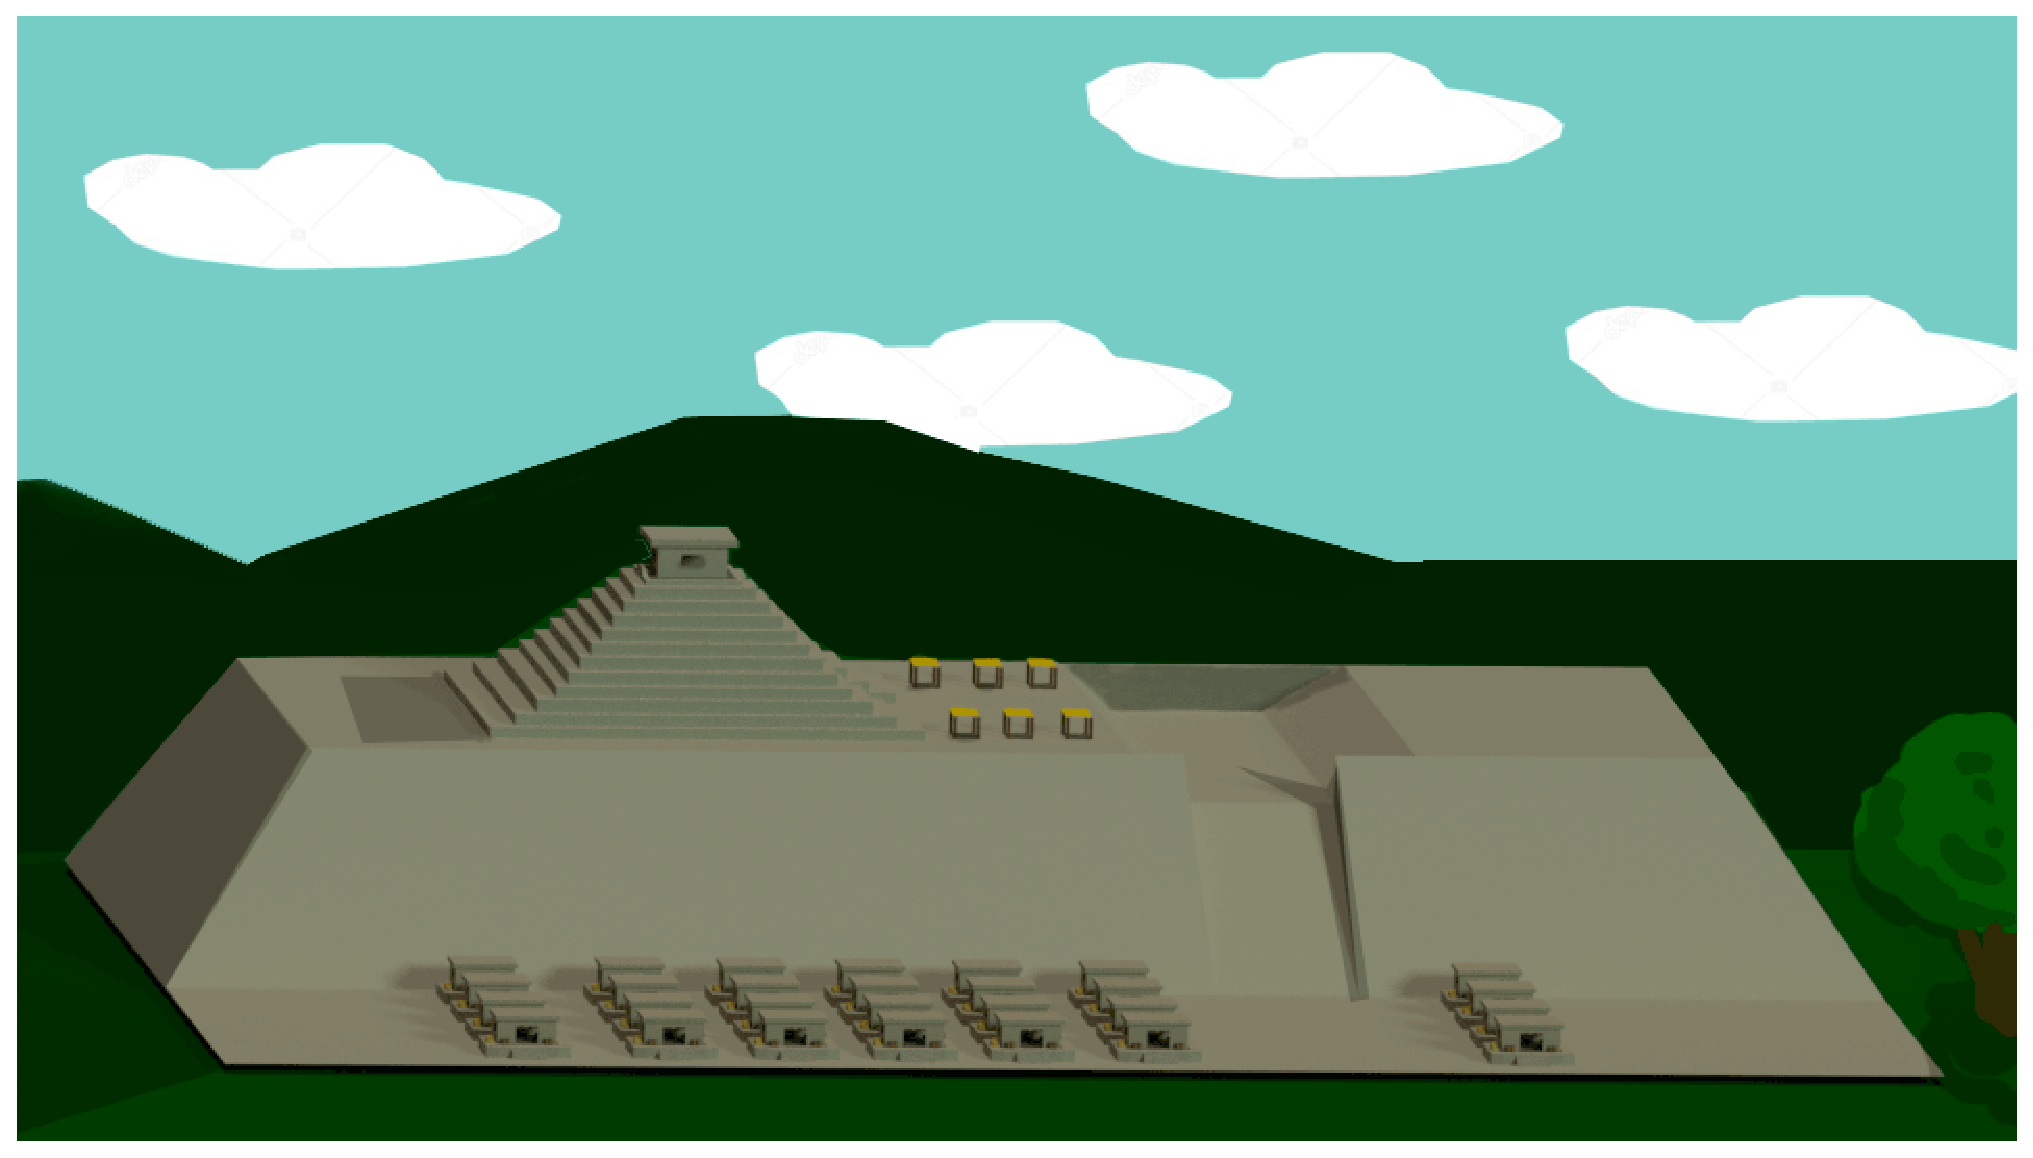
\includegraphics[width=0.6\textwidth]{09Anexos/sprites/fondo02}
\end{center}

\begin{center}
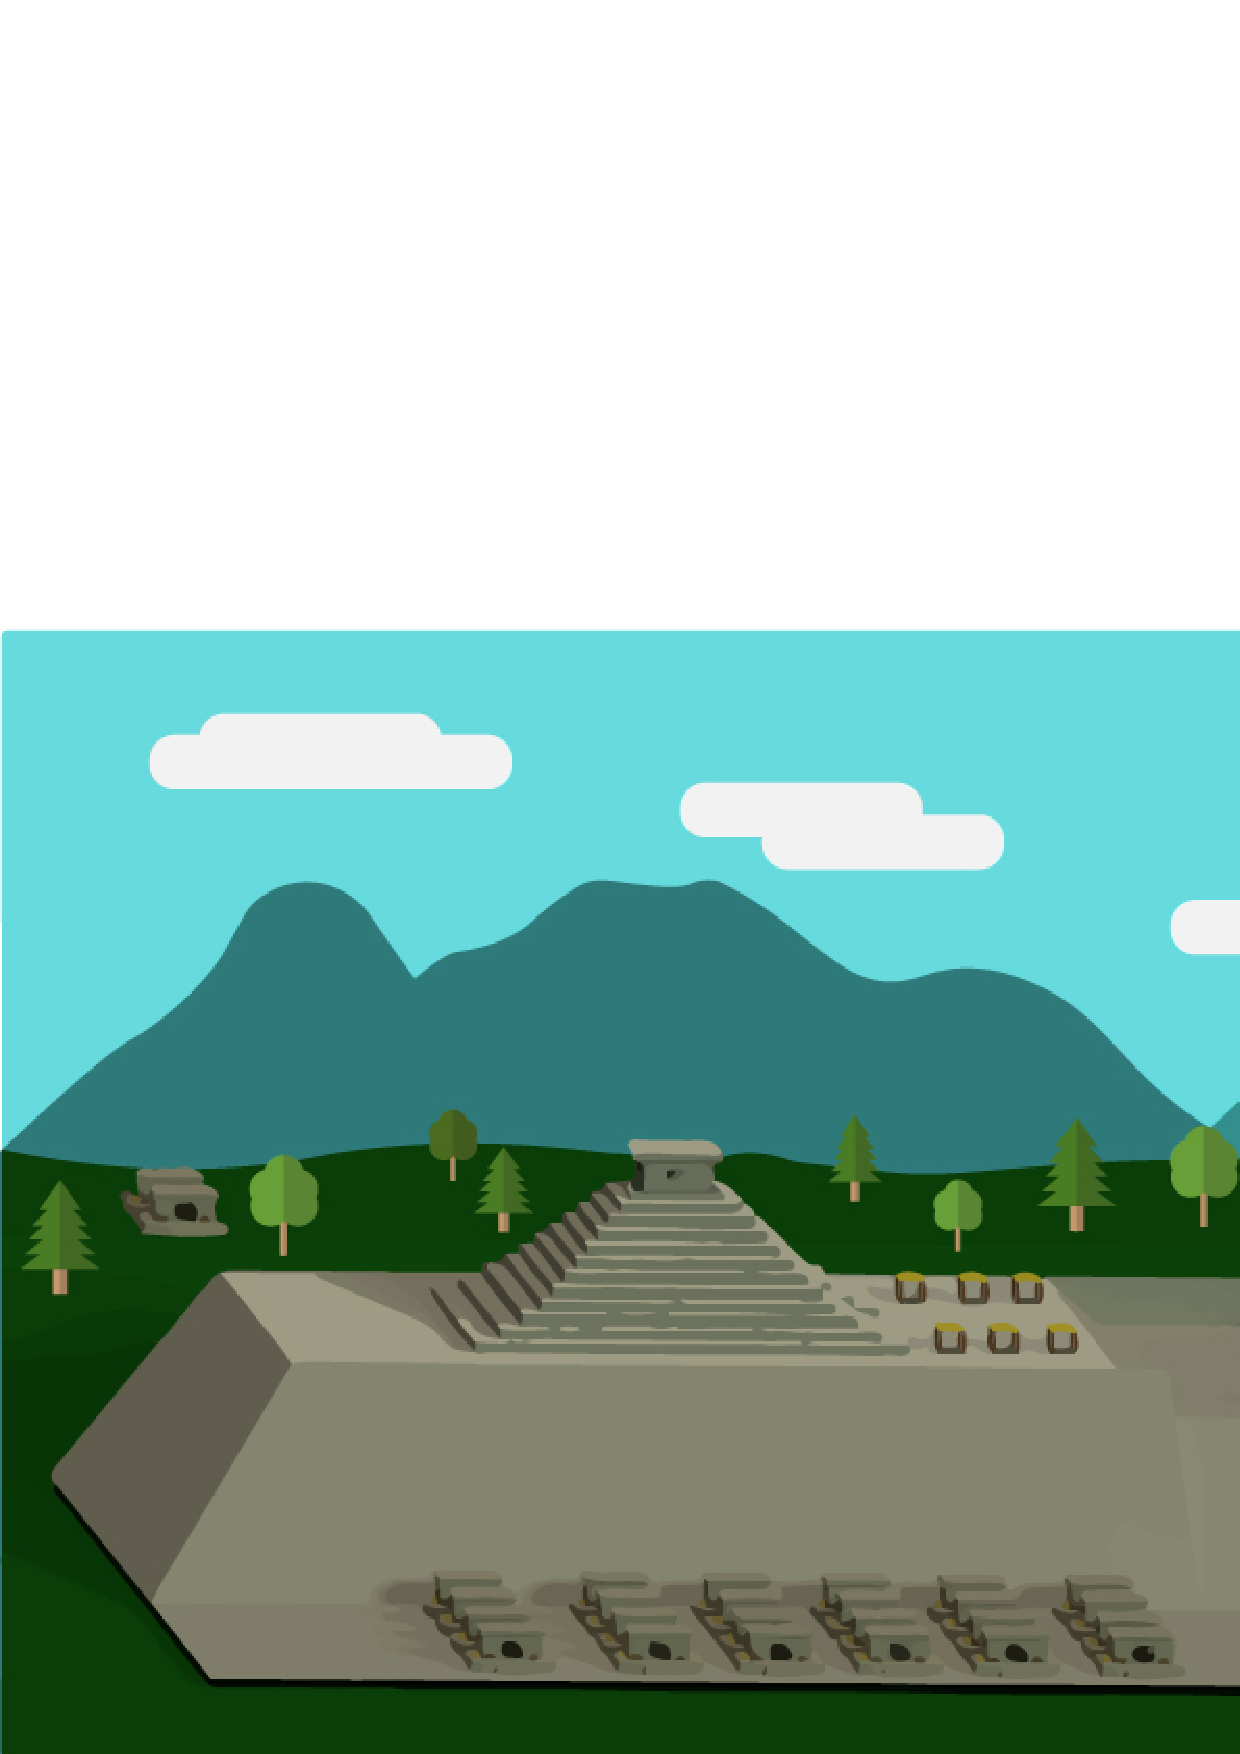
\includegraphics[width=0.6\textwidth]{09Anexos/sprites/fondo-Mont}
\end{center}

\begin{center}
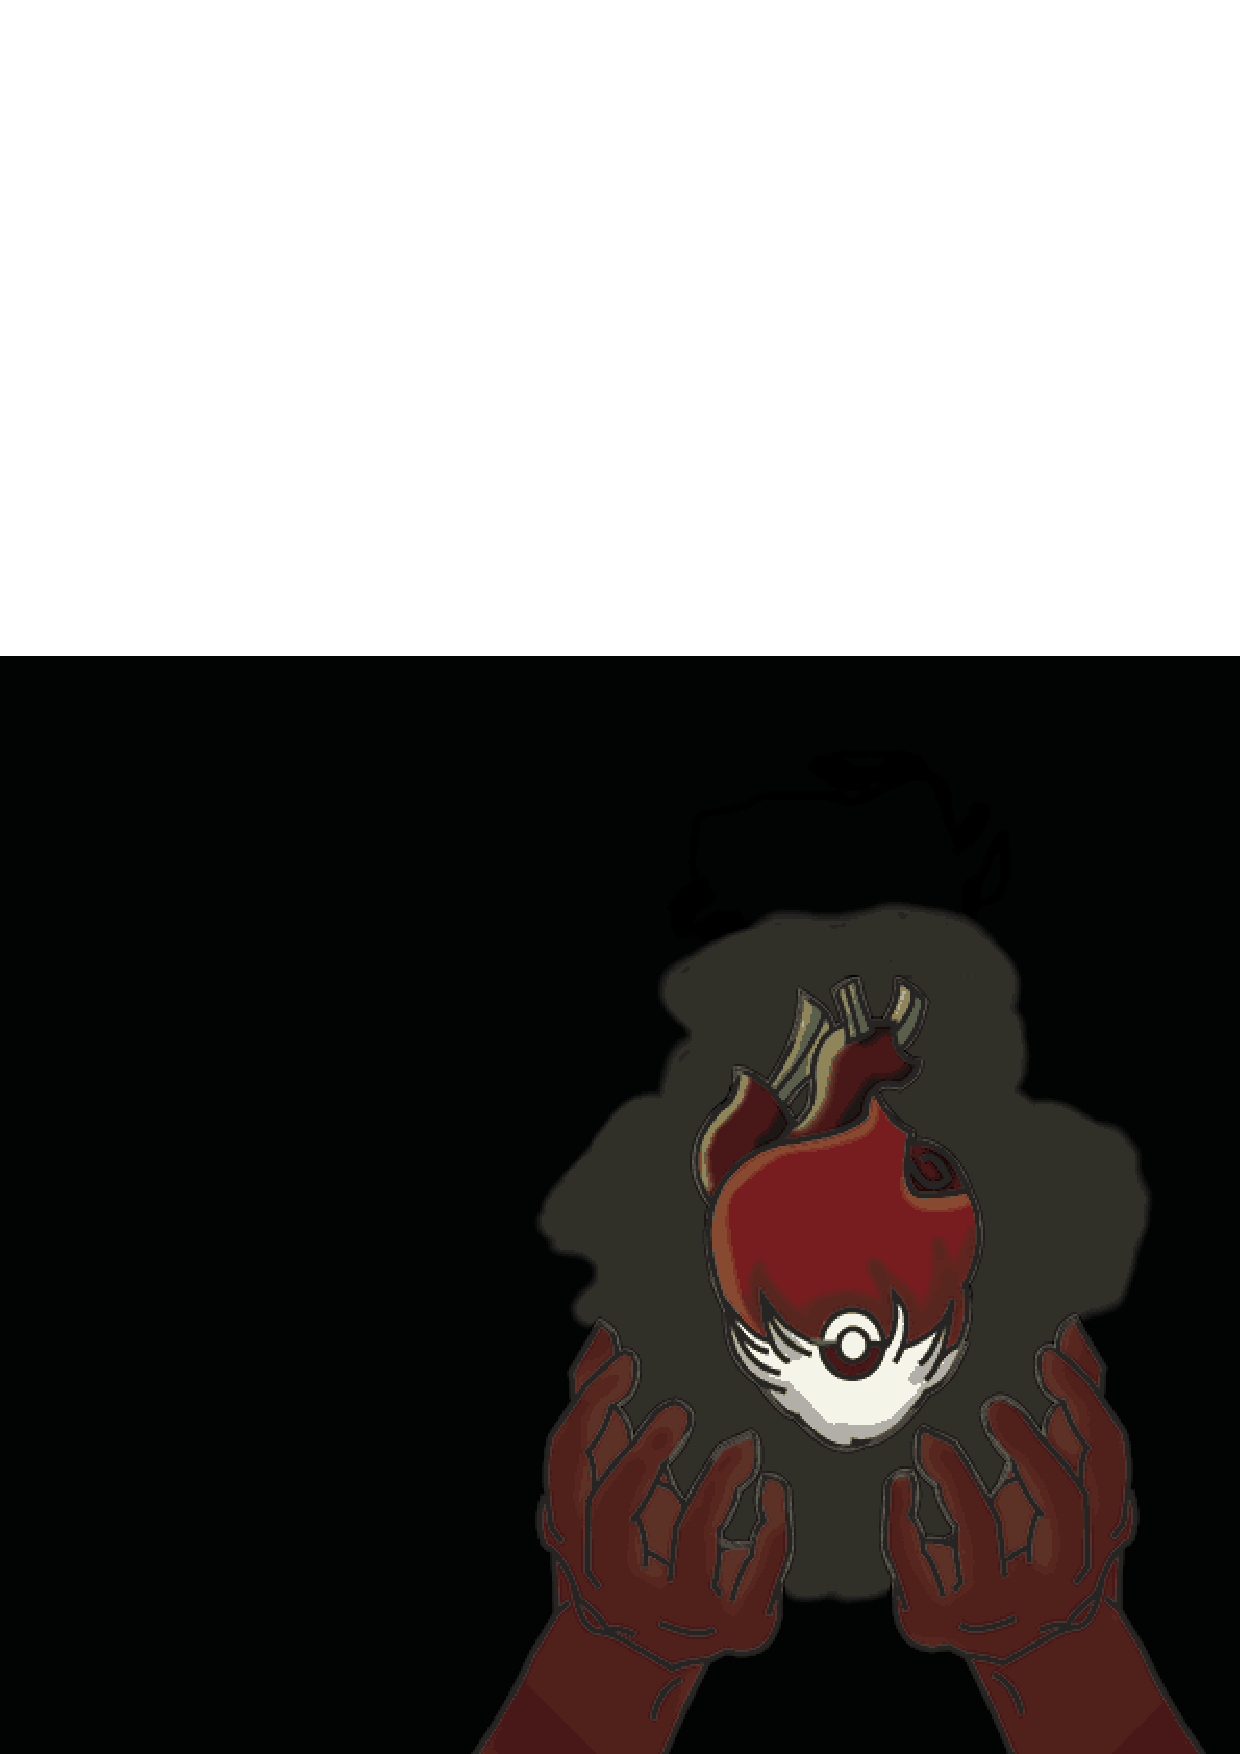
\includegraphics[width=0.6\textwidth]{09Anexos/sprites/yolotl_logo}
\end{center}

\subsection{Personajes}
En esta sección de muestran algunas de las imagenes para los personajes del juego que se crearon:
\\
\par
\begin{center}
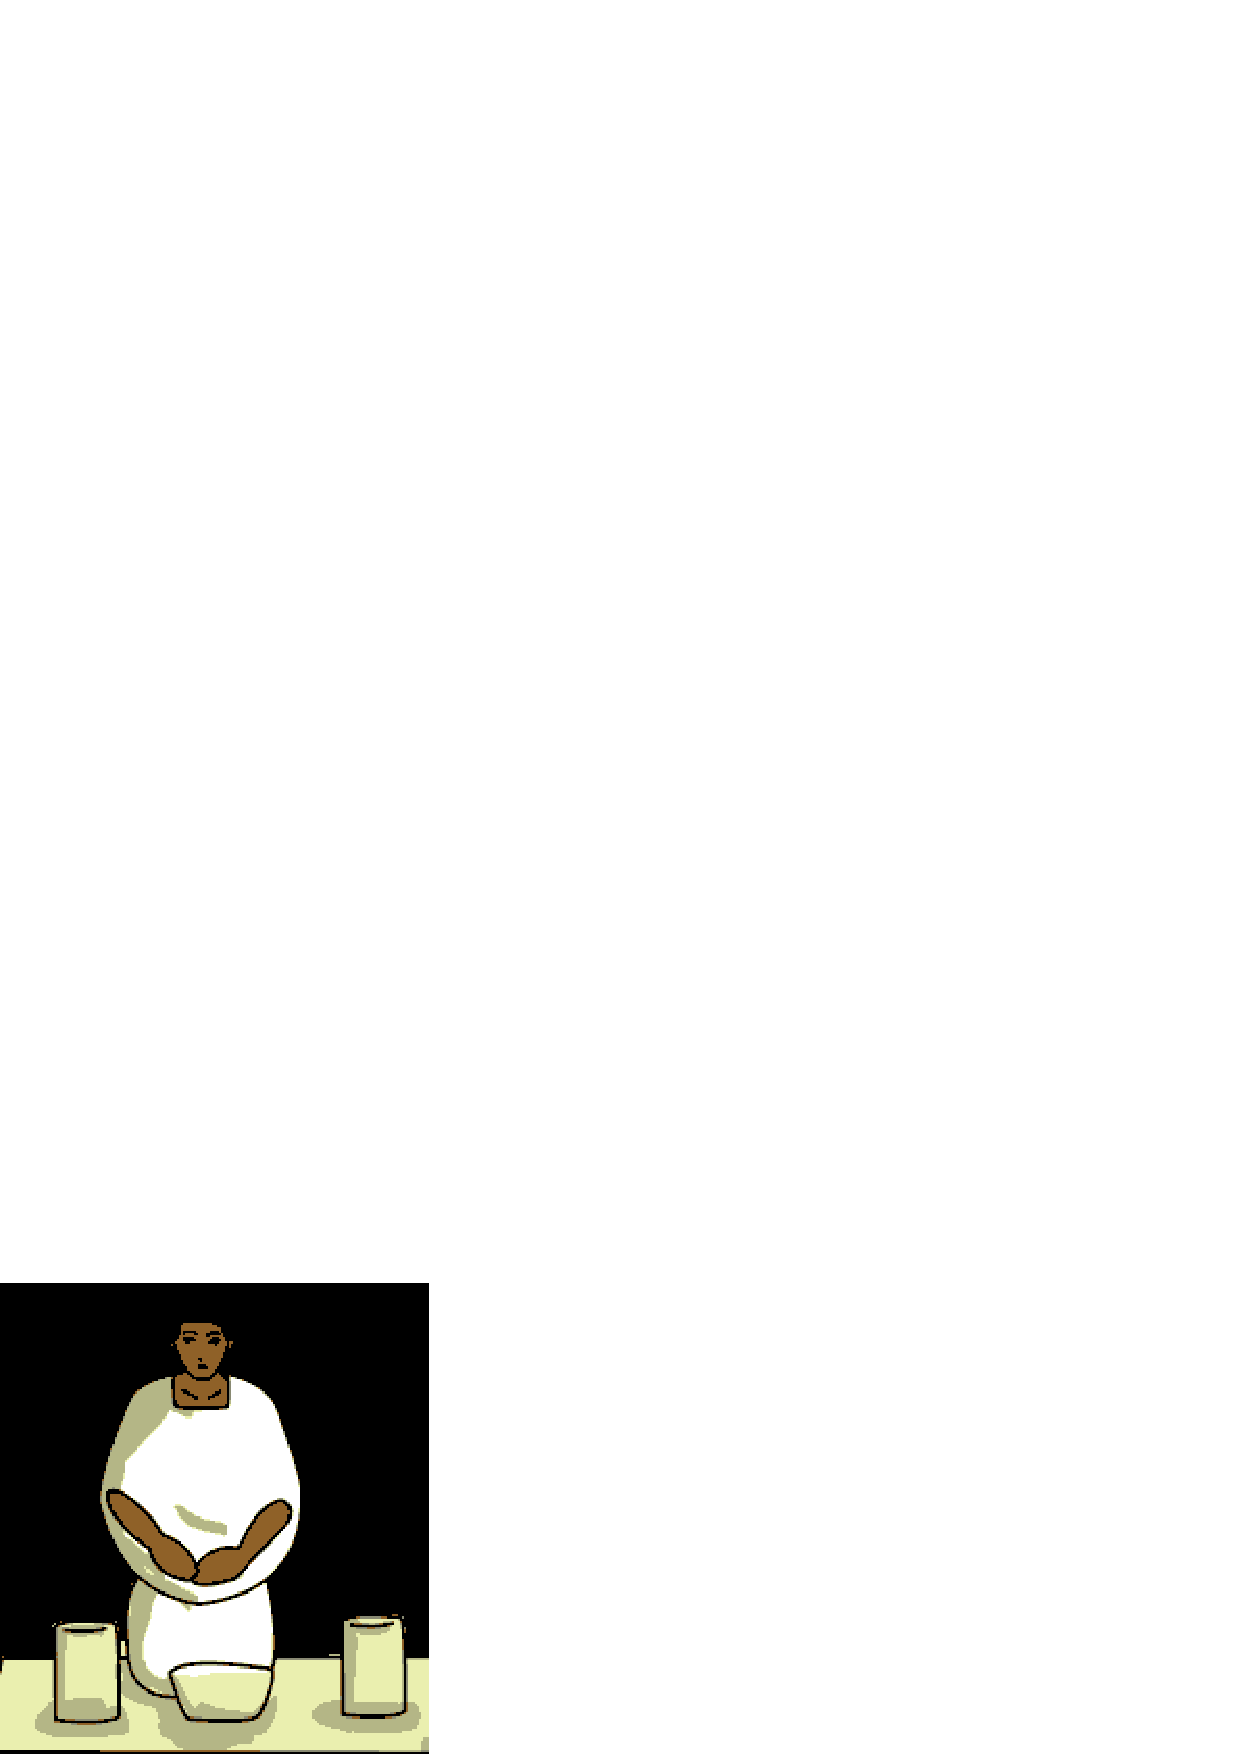
\includegraphics[width=0.3\textwidth]{09Anexos/sprites/mujer02}
\end{center}

\begin{center}
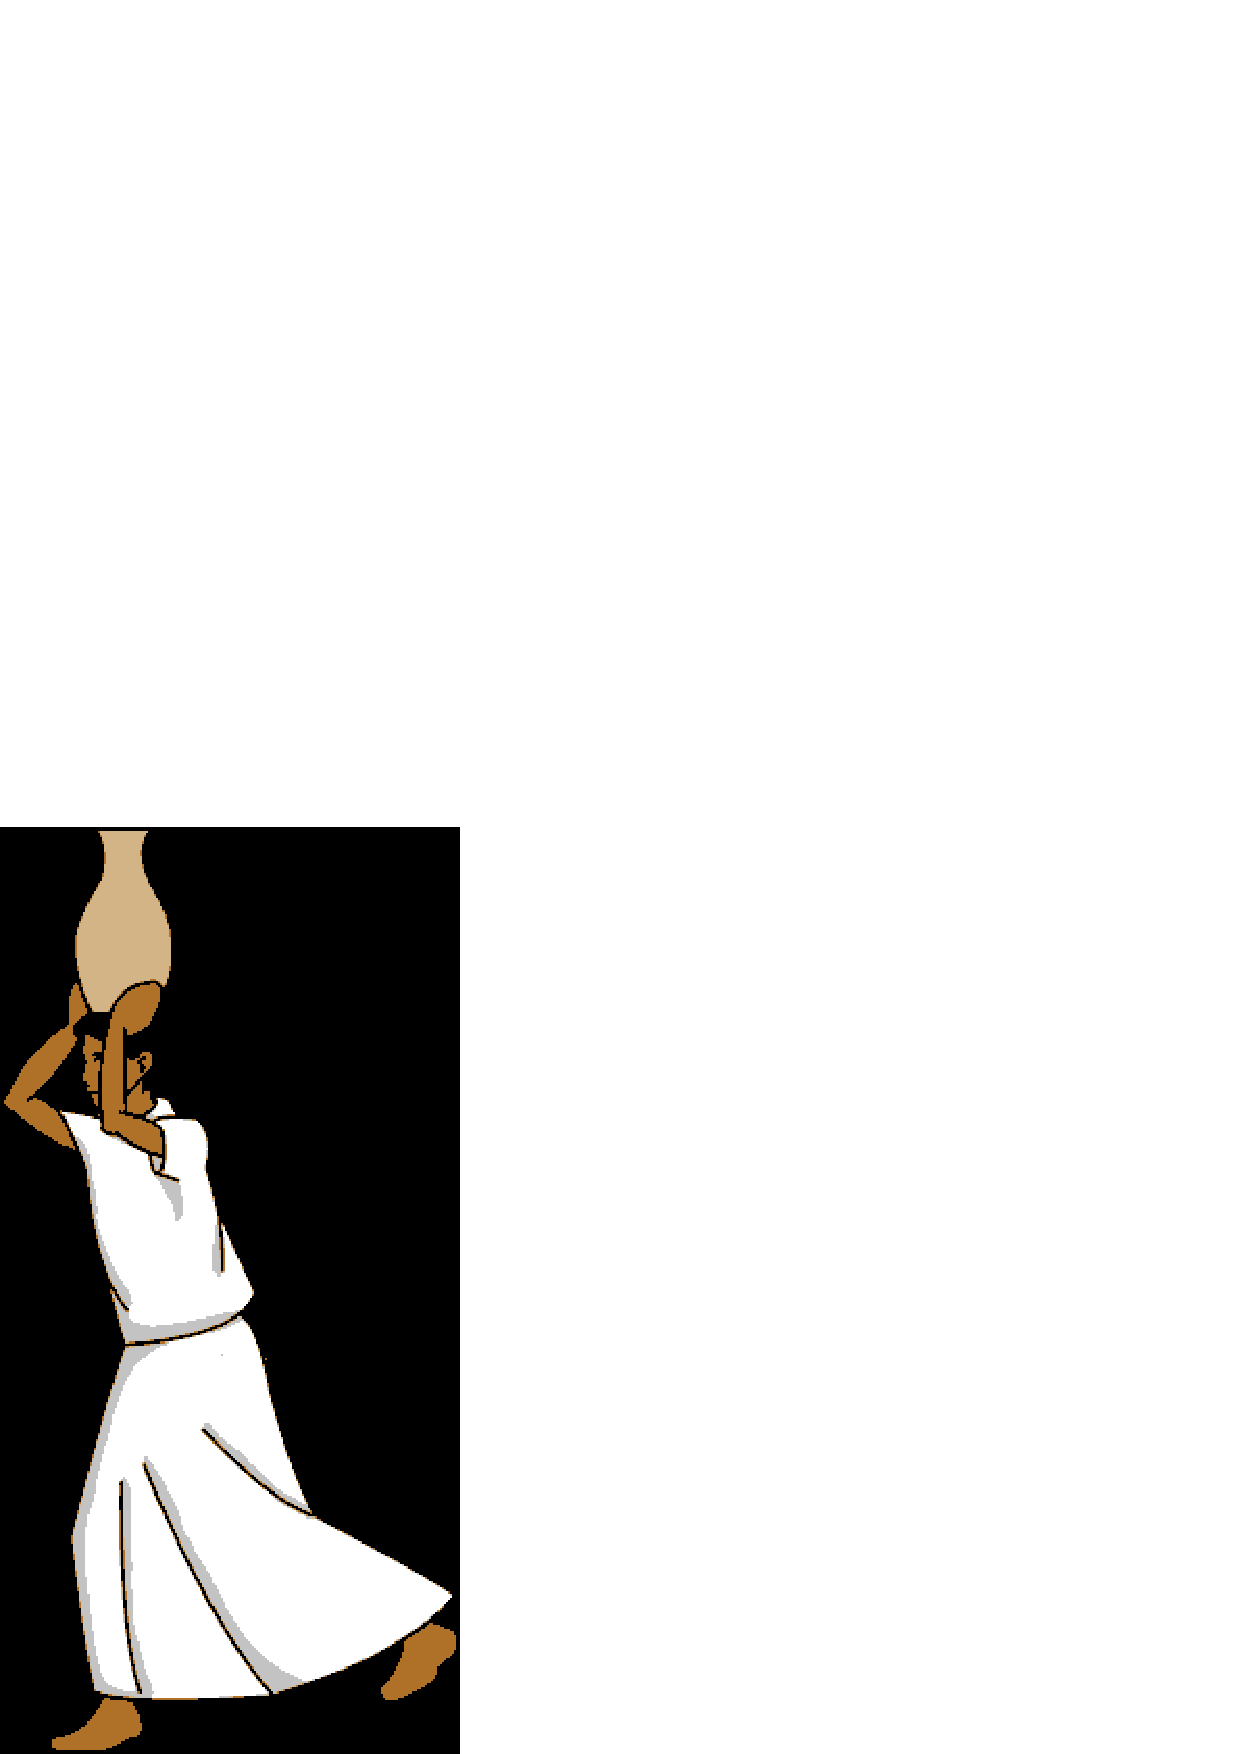
\includegraphics[width=0.1\textwidth]{09Anexos/sprites/muujer01}
\end{center}

\begin{center}
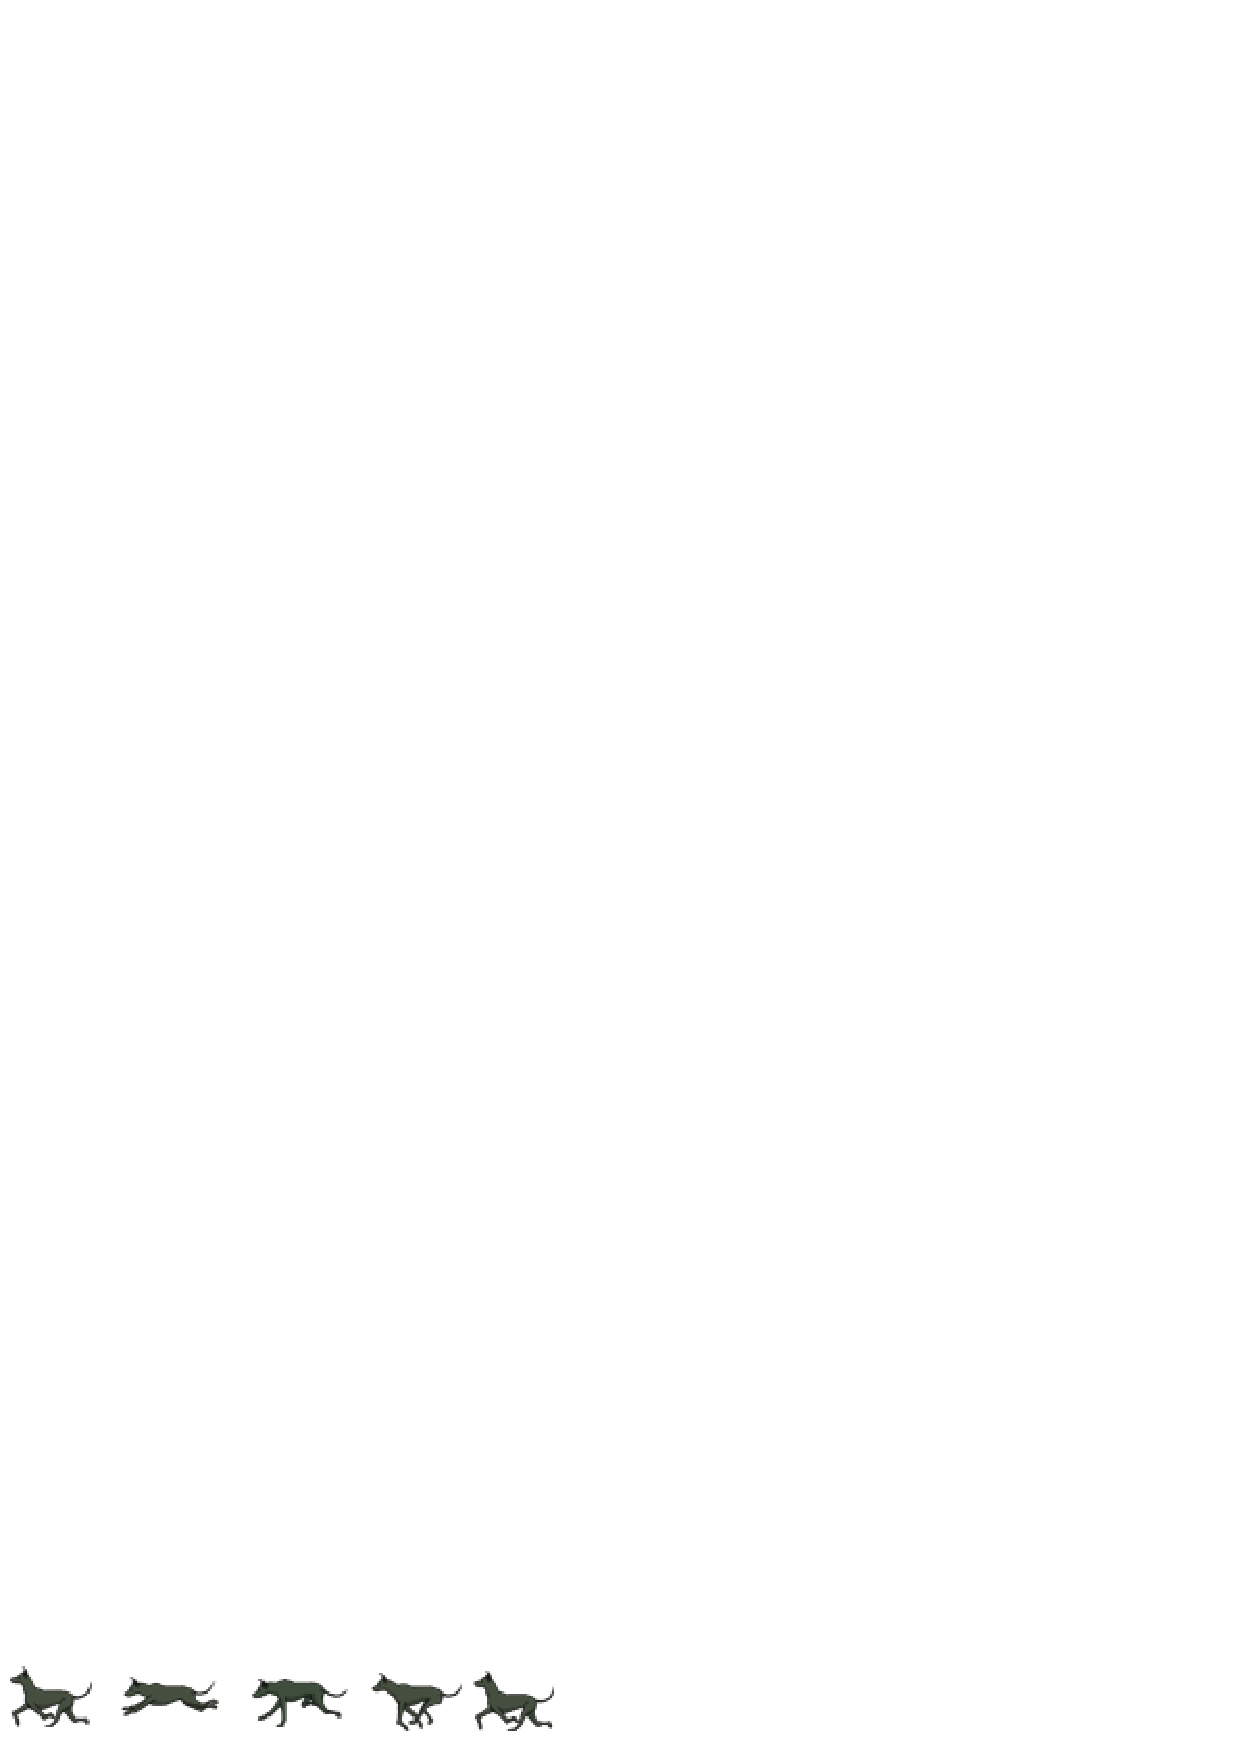
\includegraphics[width=0.7\textwidth]{09Anexos/sprites/xolotlAnimacion}
\end{center}
\section{Maquetas}
En esta sección se muestran las maquetas referentes al nivel 1 y al nivel 2.

\subsection{Maqueta nivel 1}\label{Mac01}
Maquetado del nivel 21.
\begin{center}
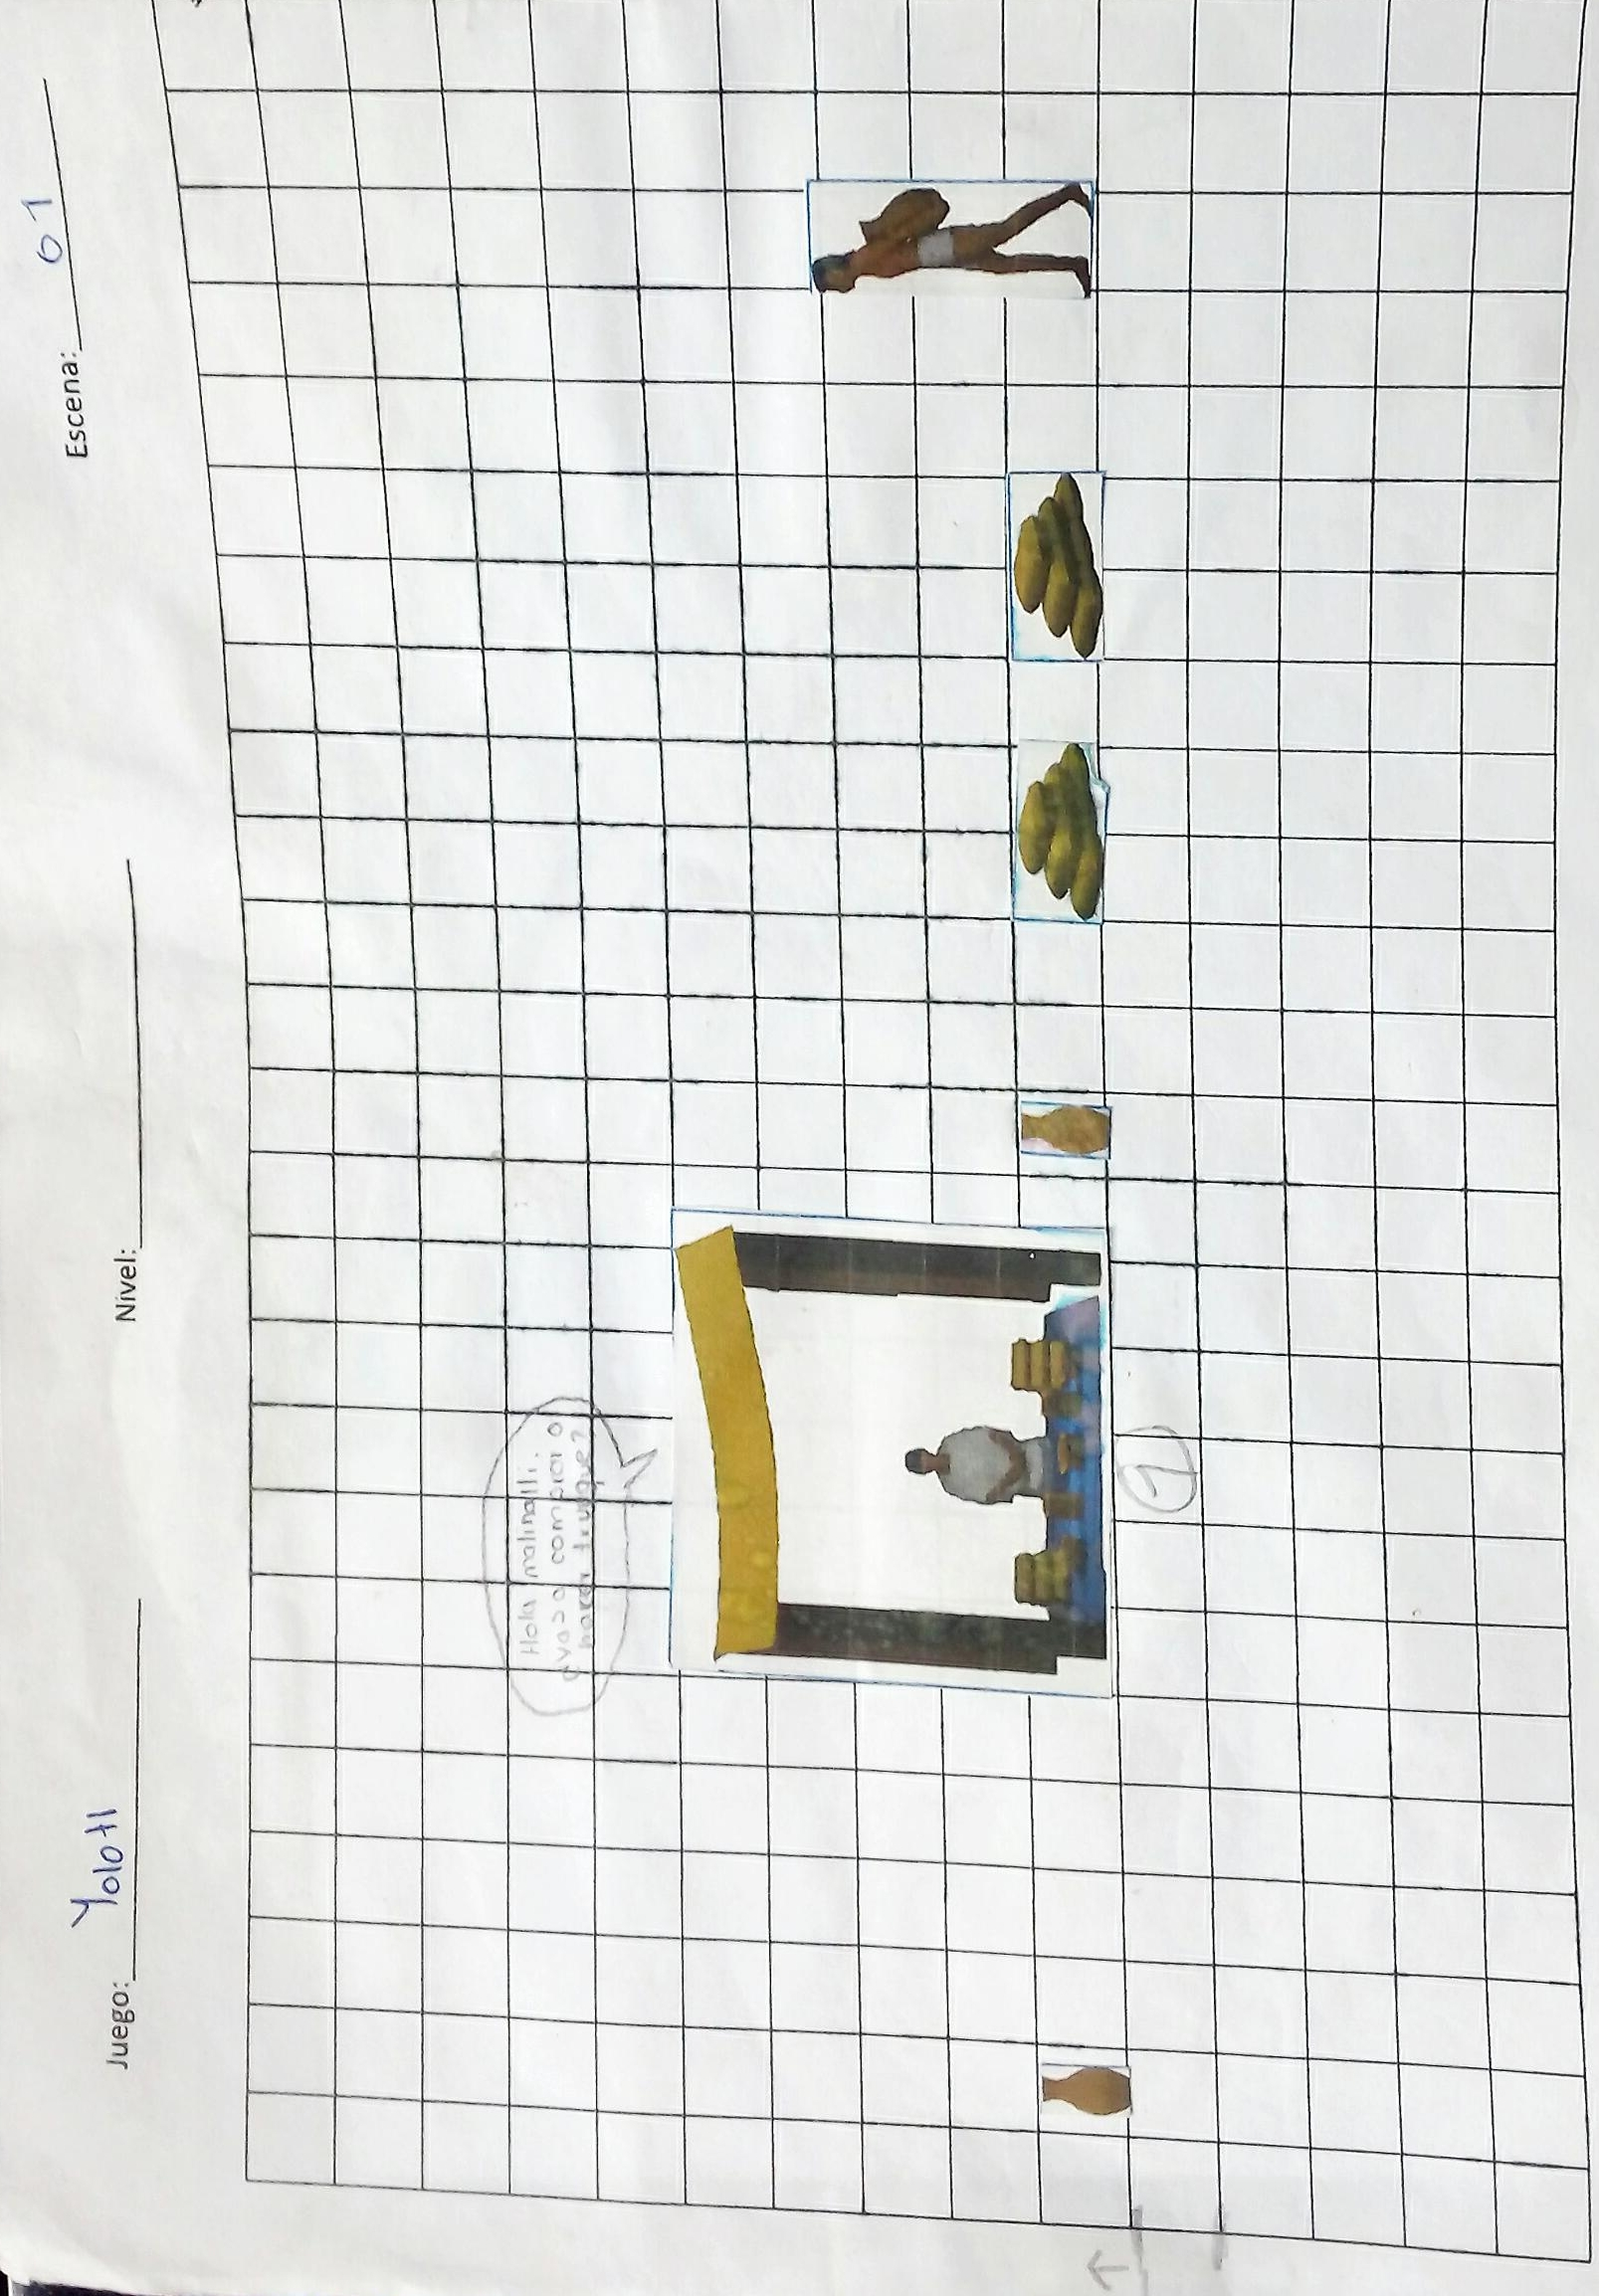
\includegraphics[width=0.9\textwidth]{09Anexos/sprites/M0101}
\end{center}

\begin{center}
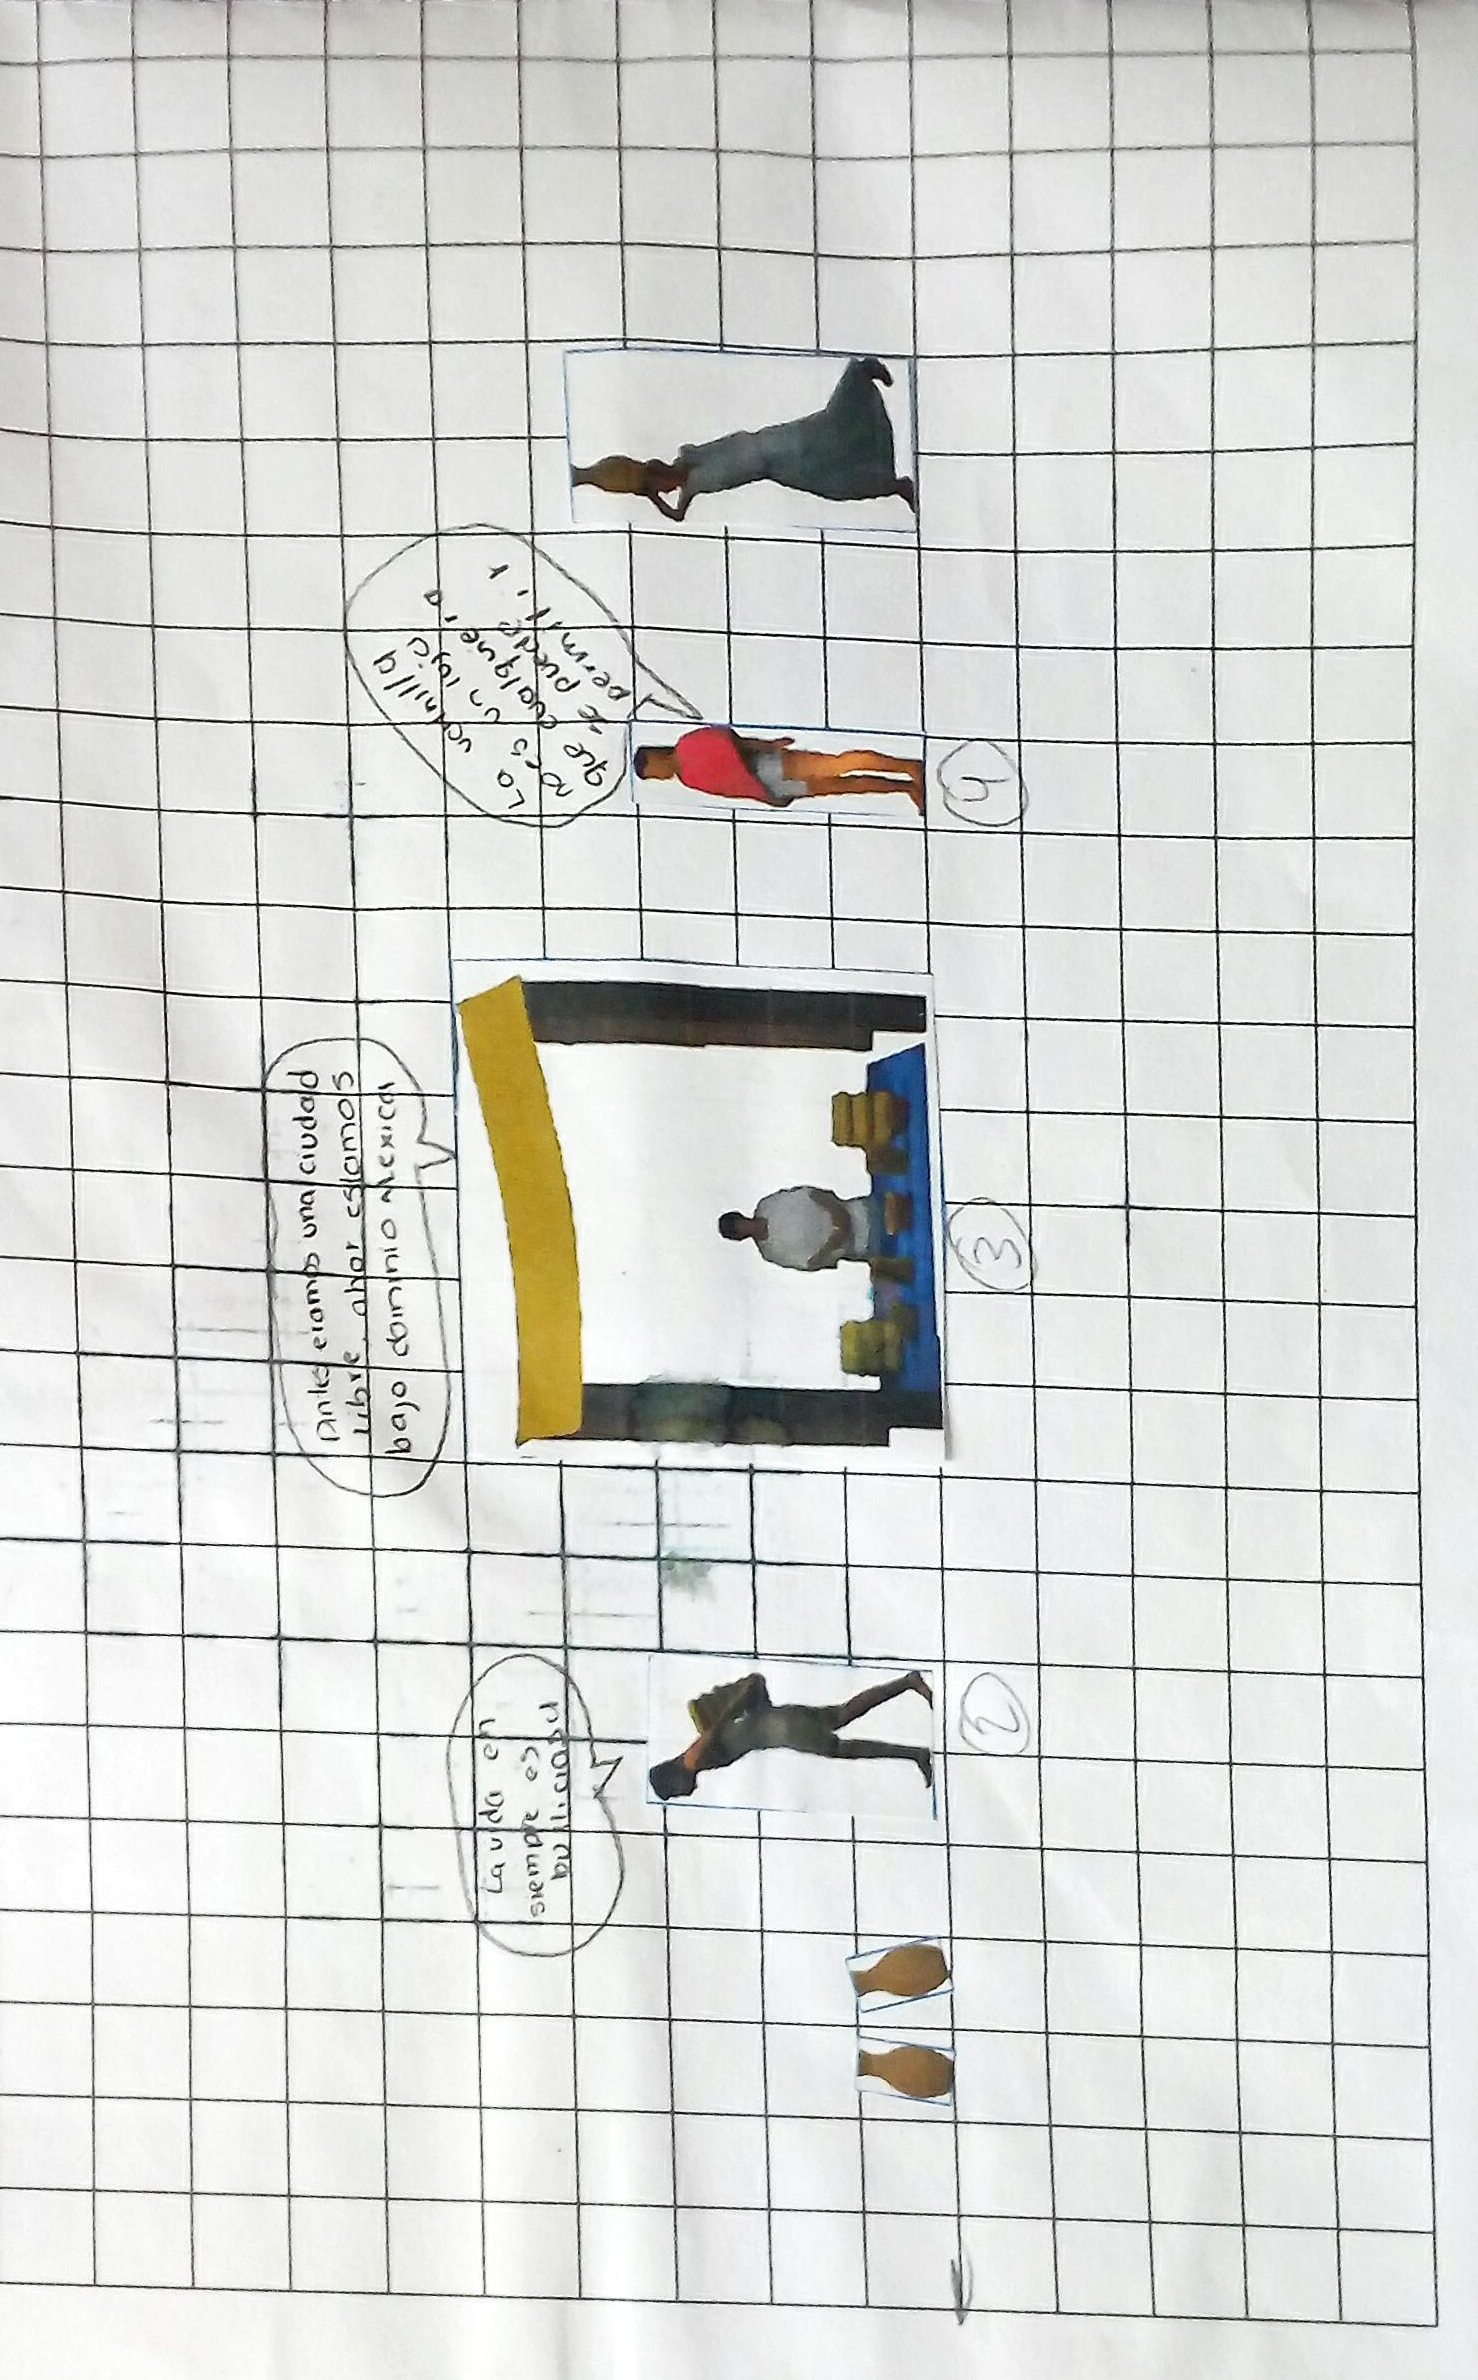
\includegraphics[width=0.9\textwidth]{09Anexos/sprites/M0102}
\end{center}

\begin{center}
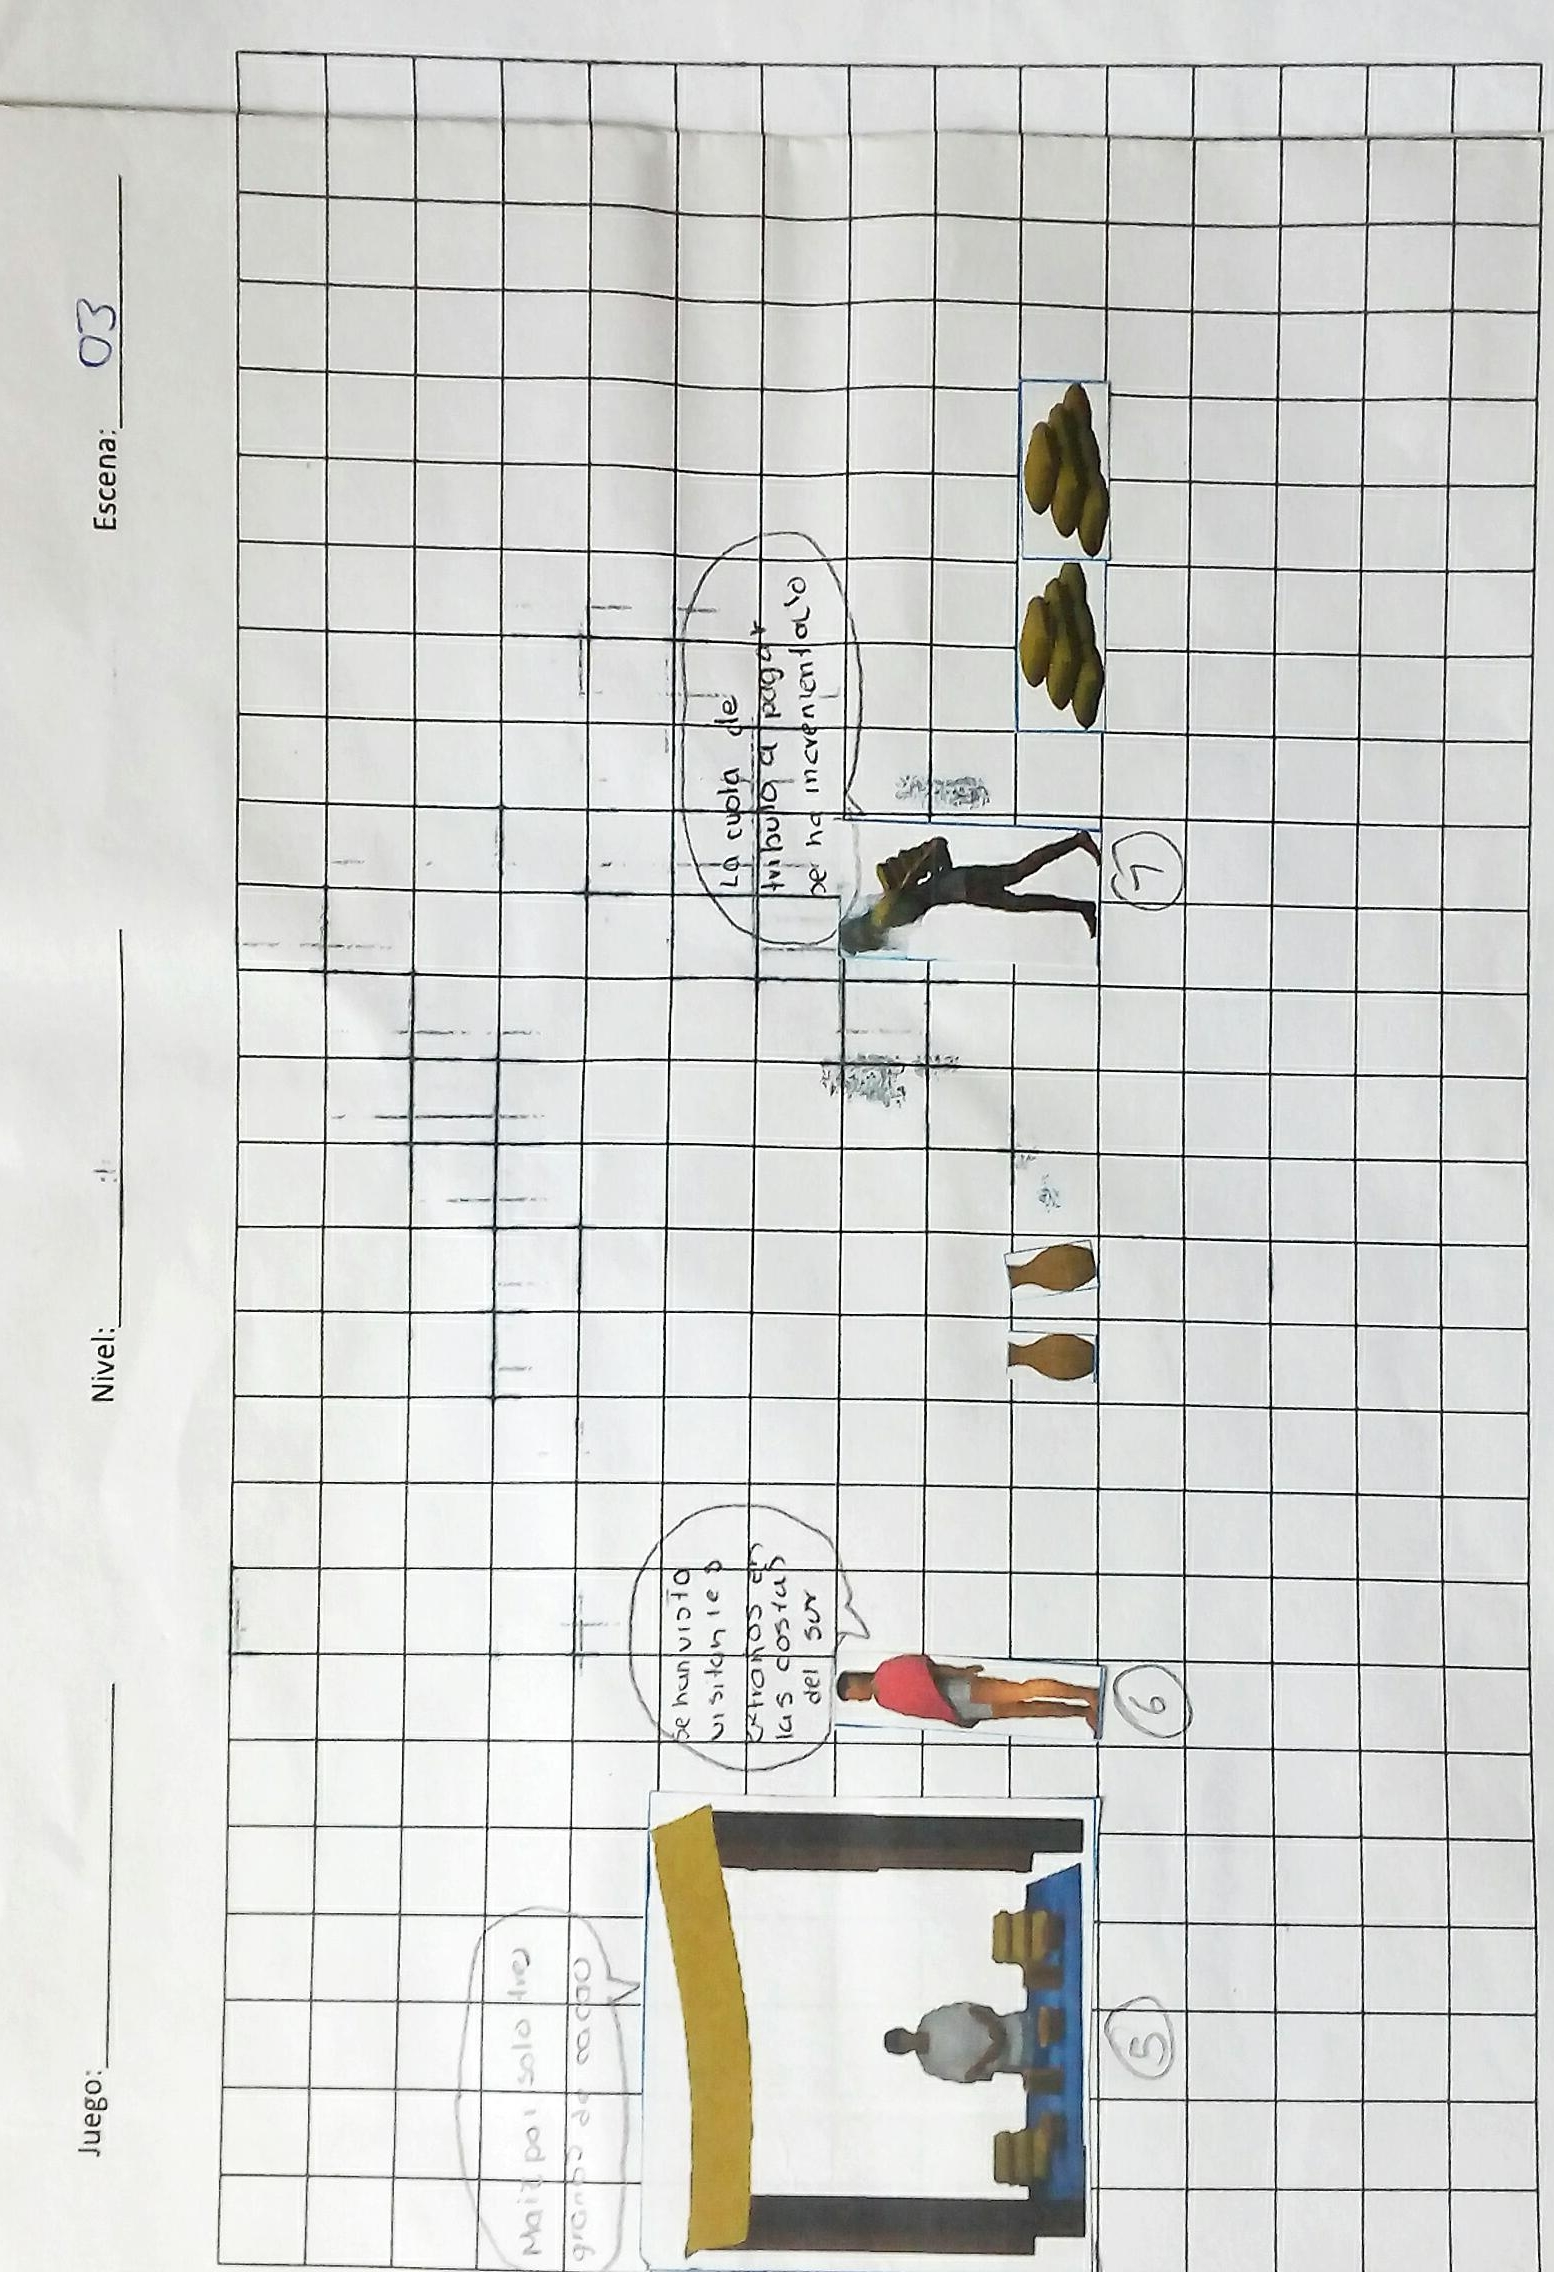
\includegraphics[width=0.9\textwidth]{09Anexos/sprites/M0103}
\end{center}

\begin{center}
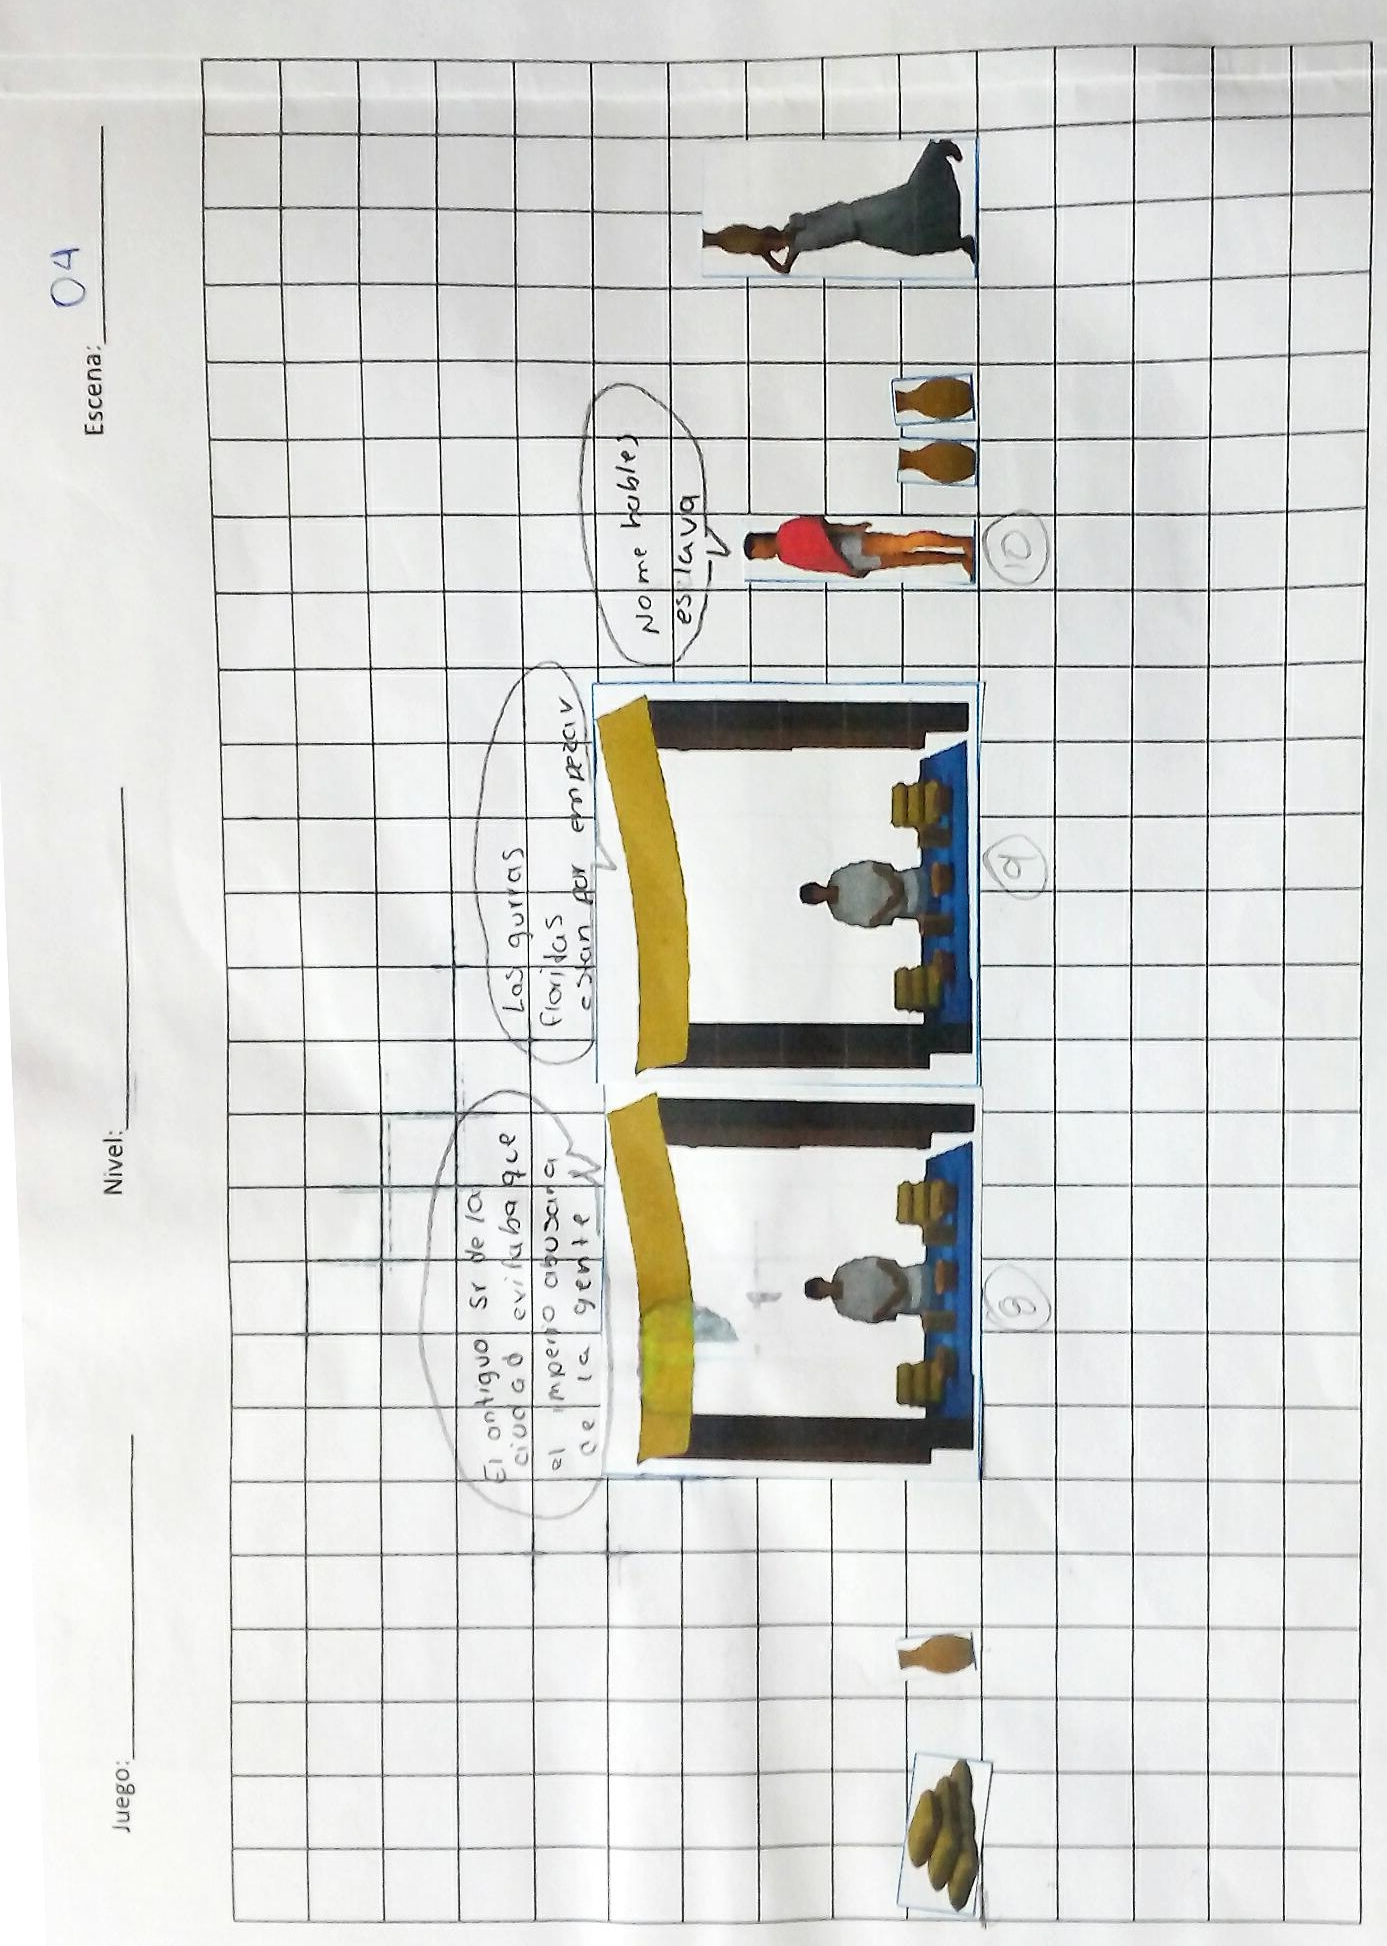
\includegraphics[width=0.9\textwidth]{09Anexos/sprites/M0104}
\end{center}

\begin{center}
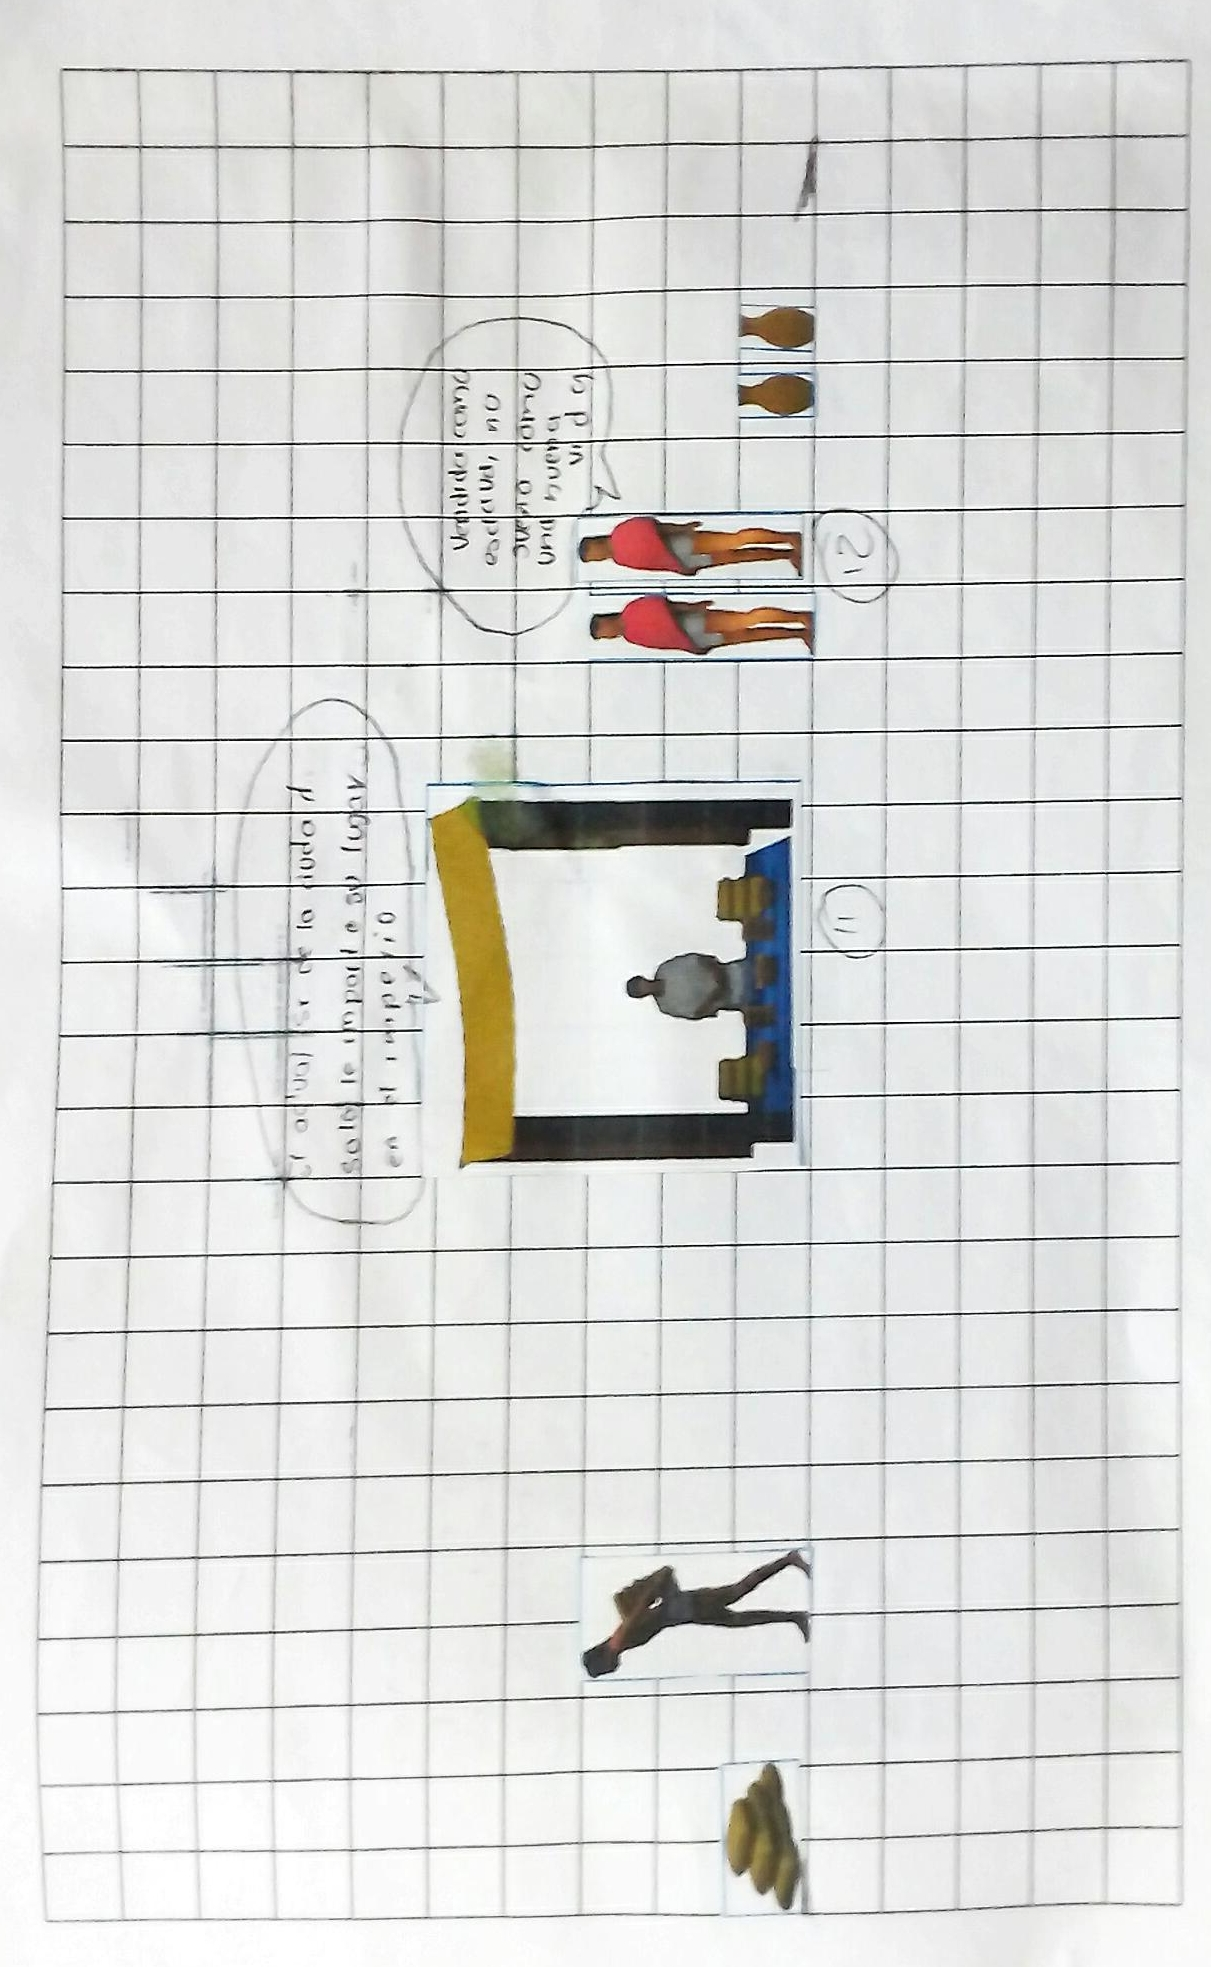
\includegraphics[width=0.9\textwidth]{09Anexos/sprites/M0105}
\end{center}


\subsection{Maqueta nivel 2}\label{Mac02}
Maquetado del nivel 2.
\begin{center}
\includegraphics[width=0.9\textwidth]{09Anexos/sprites/ML0201}
\end{center}

\begin{center}
\includegraphics[width=0.9\textwidth]{09Anexos/sprites/ML0202}
\end{center}

\begin{center}
\includegraphics[width=0.9\textwidth]{09Anexos/sprites/ML0203}
\end{center}

\begin{center}
\includegraphics[width=0.9\textwidth]{09Anexos/sprites/ML0204}
\end{center}

\begin{center}
\includegraphics[width=0.9\textwidth]{09Anexos/sprites/ML0205}
\end{center}

\begin{center}
\includegraphics[width=0.9\textwidth]{09Anexos/sprites/ML0206}
\end{center}

\begin{center}
\includegraphics[width=0.9\textwidth]{09Anexos/sprites/ML0207}
\end{center}

\begin{center}
\includegraphics[width=0.9\textwidth]{09Anexos/sprites/ML0208}
\end{center}

\begin{center}
\includegraphics[width=0.9\textwidth]{09Anexos/sprites/ML0209}
\end{center}

\begin{center}
\includegraphics[width=0.9\textwidth]{09Anexos/sprites/ML0210}
\end{center}
	
\end{document}